%Document vide aux normes de l'École nationale des Chartes
%crée par J.B. Camps
%Dernières modifications E. Rouquette (03/2026)

%%%%%%%%%%%%%%%%%%%%%%%%%%%%%%%%%%%%%%%%%%%%%%%%%%
%%%%%%%%%%%%%%%%%%%%%%PRÉAMBULE%%%%%%%%%%%%%%%%%%%
%%%%%%%%%%%%%%%%%%%%%%%%%%%%%%%%%%%%%%%%%%%%%%%%%%


%%%%%%%%%%%%%% partie obligatoire du préambule %%%%%%%%%%%%%%
%%%%%%%%%%%%%%%%%%%%%%%%%%%%%%%%%%%%%%%%%%%%%%%%%%%%%%%%%%%%%

\documentclass[12pt,twoside]{book}
\usepackage{fontspec}
\usepackage{xunicode}
\usepackage{polyglossia}
\setmainlanguage{french}%indiquer la langue principale du document
%\setotherlanguage{} %indiquer les autres langues utilisée

%%%%%%%%%%%%%%%%%%%PACKAGES UTILISÉS%%%%%%%%%%%%%%%%%%%
%%%%%%%%%%%%%%%%%%%%%%%%%%%%%%%%%%%%%%%%%%%%%%%%%%%%%%%

\usepackage{csquotes} % les guillemets français
\usepackage{lettrine} %faire une lettrine

%%%%%%%%%%%%%%%%%%% GESTION TYPOGRAPHIQUE & OVERFULL/UNDERFULL %%%%%%%%%%%%%%%%%%%
%%%%%%%%%%%%%%%%%%%%%%%%%%%%%%%%%%%%%%%%%%%%%%%%%%%%%
\usepackage{microtype} %Ajustement discret de la largeur des caractères et l'espacement entre eux.
\setlength{\hfuzz}{1pt} % Indique à LaTeX d'ignorer les dépassements inférieurs à 1 pt.
\setlength{\vfuzz}{15pt} % Tolère un dépassement vertical
\emergencystretch=1.5em  % Autorise à étirer un peu un mot
\hbadness=2000 %Remonte le seuil d'alerte pour les lignes trop aérées
%%%%%%%%%%%%%%%%%%% BIBLIOGRAPHIE %%%%%%%%%%%%%%%%%%%
%%%%%%%%%%%%%%%%%%%%%%%%%%%%%%%%%%%%%%%%%%%%%%%%%%%%%

\usepackage[backend=biber,style=enc,sorting=nyt,maxbibnames=10]{biblatex}%charger le style de l'EnC (téléchargeable ici https://ctan.org/pkg/biblatex-enc)
\DeclareFieldFormat{citetitle}{\textit{#1}}% cite automatiquement les titres en italiques

% Ajout des différents fichiers bibliographiques.
\addbibresource{./bibliographie/cujas.bib}
\addbibresource{./bibliographie/numerisation.bib}
\addbibresource{./bibliographie/donnees_metadonnees.bib}
\addbibresource{./bibliographie/methodologie.bib} %Exemple de chemin à partir du dossier où se trouve le document maître:Exemple ./dossierA/fichier.bib
%\defbibheading{}{\subsection*{}} Si l'on veut changer le titre de la/les bibliographie(s)

%%%%%%%%%%%%%%%%%%%%%%%%%%%%% INDEX %%%%%%%%%%%%%%%%%%%%%%%%%%%%%%
%%%%%%%%%%%%%%%%%%%%%%%%%%%%%%%%%%%%%%%%%%%%%%%%%%%%%%%%%%%%%%%%%%

\usepackage{imakeidx} %pour faire un ou plusieurs index
\makeindex %commande pour générer l'index


%%%%%%%%%%%%%%%%%%%%%%%%%%% ABBRÉVIATIONS %%%%%%%%%%%%%%%%%%%%%%%%%%%
%%%%%%%%%%%%%%%%%%%%%%%%%%%%%%%%%%%%%%%%%%%%%%%%%%%%%%%%%%%%%%%%%%%%%

%Ce package permet de générer automatiquement des listes d'acrononyme.
\usepackage{acro}

\DeclareAcronym{ABES}{short= ABES, long = Agence bibliographique de l'enseignement supérieur}
\DeclareAcronym{API}{short = API, long = \textit{Application Programming Interface}}
\DeclareAcronym{API REST}{short = API REST, long = \textit{Application Programming Interface Representation State Transfer}}
\DeclareAcronym{ARK}{short = ARK, long = Archival Resource Key}
\DeclareAcronym{BU}{short = BU, long = \textit{Bibliothèque universitaire}}
\DeclareAcronym{BIS}{short = BIS, long = \textit{Bibliothèque interuniversitaire de la Sorbonne}}
\DeclareAcronym{BIU Cujas}{short = BIU Cujas, long = Bibliothèque interuniversitaire Cujas}
\DeclareAcronym{BNF}{short = BnF, long = Bibliothèque nationale de France}
\DeclareAcronym{BSG}{short = BSG, long = Bibliothèque Sainte-Geneviève}
\DeclareAcronym{CADIST}{short = CADIST, long = Centre d'acquisition et de diffusion de l'information scientifique et technique}
\DeclareAcronym{CINES}{short = CINES, long = Centre informatique national de l'enseignement supérieur}
\DeclareAcronym{CMS}{short = CMS, long = \textit{Content Management System}}
\DeclareAcronym{CSV}{short = CSV, long = \textit{Comma-Separated Values}}
\DeclareAcronym{DID}{short = DID, long = Département information documentaire}
\DeclareAcronym{DIT}{short = DIT, long = Département informatique technique}
\DeclareAcronym{DPCN}{short = DPCN, long = {Département du Patrimoine, de la conservation et de la numérisation}}
\DeclareAcronym{DPRE}{short = DPRE, long = Département des périodiques et des ressources électroniques}
\DeclareAcronym{ENS}{short = ENS, long = \textit{École normale Supérieure}}
\DeclareAcronym{ESR}{short = ESR, long = Enseignement Supérieur et de la Recherche}
\DeclareAcronym{HOPPE-Droit}{short = HOPPE-Droit, long = Hypothèses d'Observation des Productions Pédagogiques Editées en Droit}
\DeclareAcronym{HTML}{short = HTML, long = HyperText Markup Language}
\DeclareAcronym{IFLA-LRM}{short = IFLA-LRM, long = \textit{International Federation of Library Associations - Library Reference Model}}
\DeclareAcronym{IIIF}{short = IIIF, long = \textit{International Image Interoperability Framework}}
\DeclareAcronym{INHA}{short = INHA, long = Institut national d’histoire de l’art}
\DeclareAcronym{JPEG}{short = JPEG, long = \textit{Joint Photographic Experts Group}}
\DeclareAcronym{JSON}{short = JSON, long = \textit{JavaScript Object Notation}}
\DeclareAcronym{JSON-LD}{short = JSON-LD, long = \textit{JavaScript Object Notation for Linked Data}}
\DeclareAcronym{METS}{short = METS, long = \textit{Metadata Encoding and Transmission Standard}}
\DeclareAcronym{NAS}{short = NAS, long = \textit{Network Attached Storage}}
\DeclareAcronym{OAI-PMH}{short = OAI-PMH, long = \textit{Open Archives Initiative Protocol for Metadata Harvesting}}
\DeclareAcronym{OCR}{short = OCR, long = \textit{Optical Character Recognition}}
\DeclareAcronym{OEMI}{short = OEMI, long = \textit{Objet Expression Manifestation Item}}
\DeclareAcronym{PNG}{short = PNG, long = \textit{Portable Network Graphics}}
\DeclareAcronym{PDF}{short = PDF, long =  \textit{Portable Document Format}}
\DeclareAcronym{RAMEAU}{short = RAMEAU, long = \textit{Répertoire d'Autorité Matière Encyclopédique et Alphabétique Unifié}}
\DeclareAcronym{RDA-FR}{short = RDA-FR, long = \textit{Resource Description and Access en France} }
\DeclareAcronym{RDF}{short = RDF, long = \textit{Resource Description Framework}}
\DeclareAcronym{RIS}{short = RIS, long = \textit{Research Information Systems}}
\DeclareAcronym{SAML}{short = SAML, long = \textit{Security Assertion Markup Language}}
\DeclareAcronym{SEO}{short = SEO, long = \textit{Search Engine Optimization}}
\DeclareAcronym{SFTP}{short = SFTP, long = \textit{Secure File Transfer Protocol}}
\DeclareAcronym{SIC}{short = SIC, long = Sciences de l'Information et de la Communication}
\DeclareAcronym{SIGB}{short= SIGB, long = Système Intégré de Gestion de Bibliothèque}
\DeclareAcronym{SIP}{short = SIP, long = \textit{Session Initiation Protocol}}
\DeclareAcronym{SKOS}{short = SKOS, long = \textit{Simple Knowledge Organization System}}
\DeclareAcronym{SSO}{short = SSO, long = \textit{Single Sign-On}}
\DeclareAcronym{SQL}{short = SQL, long = \textit{Structure Query Language}}
\DeclareAcronym{SUDOC}{short = SUDOC, long = Système universitaire de documentation}
\DeclareAcronym{TDM}{short = TDM, long = \textit{Text and Data Mining}}
\DeclareAcronym{TIFF}{short = TIFF, long = \textit{Tagged Image File Format}}
\DeclareAcronym{URI}{short = URI, long = \textit{Uniform Resource Identifier}}
\DeclareAcronym{UX}{short = UX, long = \textit{User Experience}}
\DeclareAcronym{VIAF}{short = VIAF, long = \textit{Virtual International Authority File}}
\DeclareAcronym{WCAG}{short = WCAG, long = \textit{Web Content Acessibility Guidelines}}
\DeclareAcronym{XML}{short = XML, long = \textit{eXtensible Markup Language}}
\DeclareAcronym{XML-TEI}{short = XML-TEI, long = \textit{eXtensible Markup Language - Text Enconding Initiative}}
\DeclareAcronym{XTF}{short = XTF, long = \textit{eXtensible Text Framework}}

%%%%%%%%%%%%%%%%%%% CONFIGURATION DE MISE EN PAGE %%%%%%%%%%%%%%%%%%%
%%%%%%%%%%%%%%%%%%%%%%%%%%%%%%%%%%%%%%%%%%%%%%%%%%%%%%%%%%%%%%%%%%%%%

%%%%%% Les compteurs (sections, subsections, etc)
%\renewcommand{\thesection}{\Roman{section}.}%On ne fait apparaître que le numéro de la section
\renewcommand{\thesection}{\thechapter.\arabic{section}}
\renewcommand{\thesection}{\arabic{section}.}% Numérotation de la subsection en chiffre
\renewcommand{\thesubsection}{\arabic{section}.\arabic{subsection}}% Numérotation de la subsubsection pour obtenir le résultat suivant (4.1.1)
\renewcommand{\thesubsubsection}{\thesubsection.\arabic{subsubsection}}
%Si l'on veut faire apparaître les subsubsection dans le table des matières (à commenter sinon)
\setcounter{tocdepth}{3}
\setcounter{secnumdepth}{3}  % La subsubsection (profondeur=3 dans la table des matières) apparait numérotée dans la TdM

%%%%%% Création de l'arborescence des différents titres
\usepackage{titlesec}
\titleformat{\subsection}{\normalfont\large\bfseries\raggedright}{\thesubsection}{1em}{}
% Indentation des sous-sections (ex: 2.1)
\titlespacing*{\subsection}{0.5cm}{3.25ex plus 1ex minus .2ex}{1.5ex plus .2ex}

% Indentation encore plus poussée des subsubsections (ex: 2.1.1)
\titlespacing*{\subsubsection}{1cm}{3.25ex plus 1ex minus .2ex}{1.5ex plus .2ex}
%Indentation des paragraphes
\titlespacing*{\paragraph}{1.5cm}{3.25ex plus 1ex minus .2ex}{1.5ex plus .2ex}

% Force le paragraphe à sauter une ligne après son titre
\titleformat{\paragraph}[hang]{\normalfont\bfseries}{\theparagraph}{1em}{}
%%%%%  Configurer le document selon les normes de l'école

\usepackage[margin=2.5cm]{geometry} %marges
\usepackage{setspace} % espacement qui permet ensuite de définir un interligne
\onehalfspacing % interligne de 1.5
\setlength\parindent{1cm} % indentation des paragraphes à 1 cm


%%%%% Mise en forme des headers (haut de page)

\usepackage{fancyhdr} %package utilisé pour modifier les headers
\pagestyle{fancy} %utiliser ses propres choix de mise en page et non ceux par défaut du package

\setlength\headheight{16pt}%la hauteur des headers

%%la façon dont les sections apparaissent dans les en-tête:

\renewcommand{\sectionmark}[1]{\markright{\small\textit{\thesection~\  #1}}}%Faire apparaître dans les headers les sections en  petit et en italiques
%\renewcommand{\sectionmark}[1]{}%Commenter la lign précédetne et mettre celle-ci pour ne pas avoir le titre des sections dans le header

%% réglages propres à frontmatter

\appto\frontmatter{\pagestyle{fancy}%
	\renewcommand{\chaptermark}[1]{\markboth{\small\textit{#1}}{}}% ne pas faire apparaître de <<numéro>> de chapitre dans les chapitres non numérotés (front: l'introduction, els remerciement, etc)
}

%%%%%% Mise en forme en bas de page souple
\raggedbottom % Lui indiquer qu'il n'est pas obligé d'étirer tous les textes pour que cela se finisse pareil peut laisser le vide.

%% réglages propres à mainmatter

\appto\mainmatter{
\renewcommand{\chaptermark}[1]{\markboth{\small\chaptername~\thechapter~--\ \textit{#1}}{}}%faire apparaître dans les headers les sections en  petit et en italiques
%\renewcommand{\chaptermark}[1]{}%Commenter la ligne précédente et mettre celle-ci pour ne pas avoir le titre des chapitres  dans le header
}

%% réglages propres aux annexes

\appto\appendix{
	%\renewcommand{\chaptermark}[1]{\markboth{\small~Annexe \thechapter~--\ \textit{#1}}{}}%faire apparaître dans les headers le nom des annexes
	\renewcommand{\chaptermark}[1]{}%Commenter la ligne précédente et mettre celle-ci pour ne pas avoir le titre des chapitres  dans le header
}


%indiquer des règles d'hyphénation pour des mots précis si besoin
%\begin{hyphenrules}{french}
%	\hyphenation{}
%\end{hyphenrules}


%%%%%%% Package hyperref

% A mettre après les autres appels de packages car redéfinit certaines commandes).

\usepackage[colorlinks=false, breaklinks=true, pdfusetitle, pdfsubject ={Modernisation à l'accès du patrimoine juridique}, pdfkeywords={bibliothèque numérique; Bibliothèque interuniversitaire Cujas; interopérabilité; benchmark; web de données; éditorialisation; ouverture des données; approche centrée usagers.}]{hyperref} %
\usepackage[numbered]{bookmark}%va avec hyperref; marche mieux pour les signets. l'option numbered: les signets dans le pdf sont numérotés
\usepackage{xurl} % Permet les retours à la ligne n'importe où dans les URL
\usepackage{nameref}  % Permet d'extraire automatiquement le titre de l'annexe étiquetée
% Compléter pdfsubjet et pdfkeywords
%Explication des options de hyperref (modifiables)
% hyperindex=false
% colorlinks=false: pour que le cadre des liens n'apparaisse pas à l'impression
% breaklinks permet d'avoir des liens allant sur pusieurs lignes
%pdfusetitle: utiliser \author et \title pour produire le nom et le titre du pdf


%avec overleaf, utiliser :
%\usepackage[xetex]{hyperref}
%\hypersetup{
	%	pdfauthor = {Prénom Nom},
	%	pdftitle = {titre},
	%	pdfsubject = {sujet},
	%	pdfkeywords = {premier mot-clé} {deuxième mot-clé} {troisième mot-clé} {etc}
	%}



%%%%%%%%%%%%%%%%%%%% GLOSSAIRES %%%%%%%%%%%%%%%%%%%%
%%%%%%%%%%%%%%%%%%%%%%%%%%%%%%%%%%%%%%%%%%%%%%%%%%%%

%Exception: il faut le charger APRÈS hyperref
\usepackage[toc=true]{glossaries}
\makeglossaries
%avec TexStudio: F9 pour compiler le glossaire (s'il y a aussi un index)
\loadglsentries{./backmatter/glossaire.tex}
\glsaddall %Force l'inclusion de tous les termes du glossaire


%%%%%%%%%%%%%%%%%%%%%%%%%%%%%%%%%%%%%%%%%%%%%%%%%%%%
%%%%%%%%%%%%%%%%%% ENVIRONNEMENTS %%%%%%%%%%%%%%%%%%
%%%%%%%%%%%%%%%%%%%%%%%%%%%%%%%%%%%%%%%%%%%%%%%%%%%%

\usepackage{tabularray}
\usepackage{float}
\usepackage{graphicx}
\usepackage{ulem}
\usepackage{lscape} % Charge le package pour l'orientation paysage

%%%%%%%%%%%%%%%%%% NOUVELLE COMMANDE %%%%%%%%%%%%%%%%%%
%%%%%%%%%%%%%%%%%%%%%%%%%%%%%%%%%%%%%%%%%%%%%%%%%%%%
% Commande personnalisée pour renvoyer vers une annexe dans une note de bas de page
% {m} = argument obligatoire (entre accolades)
% {o} = argument optionnel (entre crochets)
\NewDocumentCommand{\footannexe}{m o}{%
	\footnote{Voir le #1\IfValueT{#2}{ #2}}%
}
%%%%%%%%%%%%%%%%%%%%%%%%%%%%%%%%%%%%%%%%%%%%%%%%%%%%%%%%%%%%%%%%%%
%%%%%%%%%%%%%%% INFORMATIONS POUR LA PAGE DE TITRE %%%%%%%%%%%%%%%
%%%%%%%%%%%%%%%%%%%%%%%%%%%%%%%%%%%%%%%%%%%%%%%%%%%%%%%%%%%%%%%%%%
 
\author{Fanny \textsc{Suszko} - M2 TNAH}
\title{Moderniser l'accès au patrimoine juridique: Diagnostic et refonte de la bibliothèque numérique de Cujas à l'heure de la Transition bibliographique}

%%%%%%%%%%%%%%%%%%%%%%%%%%%%%%%%%%%%%%%%%%%%%%%%%%%%%%
%%%%%%%%%%%%%%%%%%%%%% DOCUMENT %%%%%%%%%%%%%%%%%%%%%%
%%%%%%%%%%%%%%%%%%%%%%%%%%%%%%%%%%%%%%%%%%%%%%%%%%%%%%

\begin{document}
	\begin{titlepage}
		\begin{center}
			
			\bigskip
			
			\begin{large}				
				ÉCOLE NATIONALE DES CHARTES\\
				UNIVERSITÉ PARIS, SCIENCES \& LETTRES
			\end{large}
			\begin{center}\rule{2cm}{0.02cm}\end{center}
			
			\bigskip
			\bigskip
			\bigskip
			\begin{Large}
				\textbf{Fanny Suszko}\\
			\end{Large}
		%selon le cas
			\begin{normalsize} \textit{licenciée ès Histoire}\\
				\textit{diplômée de master d'Histoire}
			\end{normalsize}
			
			\bigskip
			\bigskip
			\bigskip
			
			\begin{Huge}
				\textbf{Moderniser l’accès au patrimoine juridique: }\\
			\end{Huge}
			\bigskip
			\bigskip
			\begin{LARGE}
				\textbf{Diagnostic et refonte de la bibliothèque numérique de Cujas à l'heure de la Transition bibliographique}\\
			\end{LARGE}
			
			\bigskip
			\bigskip
			\bigskip
			\begin{large}
				Sous la direction de \textbf{Thomas Chaineux}
			\end{large}
			\vfill
			
			\begin{large}
				Mémoire 
				pour le diplôme de master \\
				\enquote{Technologies numériques appliquées à l'histoire} \\
				\bigskip
				2026
			\end{large}
			
		\end{center}
	\end{titlepage}

	\thispagestyle{empty}	
	\cleardoublepage
	
\frontmatter

%%%%%%%%%%%%%%%%%%%%%%%%% RESUME %%%%%%%%%%%%%%%%%%%%%%%%%%%
%%%%%%%%%%%%%%%%%%%%%%%%%%%%%%%%%%%%%%%%%%%%%%%%%%%%%%%%%%%%

	\chapter{Résumé}
\medskip
	\lettrine{À} l'ère de la transition bibliographique, les technologies numériques évoluent si rapidement qu'il devient presqu'impossible de pouvoir toutes les suivre sans l'appui d'une communauté afin d'éviter aux institutions patrimoniales de se trouver isolées à cause de services devenus obsolètes. Aujourd'hui, il est important de construire une bibliothèque numérique capable de créer des passerelles afin de participer à la valorisation des collections des institutions patrimoniales sans se trouver noyé dans la masse de données. Ce mémoire s'inscrit dans le projet de réinformatisation de la Bibliothèque Cujas à travers l'étude fine de la bibliothèque numérique actuelle, consolidée par des entretiens faisant émerger des besoins auxquels un benchmark devait permettre de répondre aux attentes aussi bien des usagers que des experts métiers de la bibliothèque. Il met en lumière l'enjeu que représente la refonte de la bibliothèque numérique notamment en terme d'interopérabilité des données, d'alignement des métadonnées sur des référentiels et d'accompagnement auprès des usagers mais aussi auprès des personnels de bibliothèques qui l'utiliseront. 
\medskip

	\lettrine{I}n the era of bibliographic transition, digital technologies are evolving at such a rapid pace that it becomes nearly impossible for heritage institutions to keep up without community support, risking technological isolation due to obsolete services. Today, it is essential to design digital libraries capable of building bridges that actively enhance the value of heritage collections without drowning in an overwhelming mass of data. This thesis is fully integrated into the system redesign and modernization project of the Cujas Library. It provides a detailed diagnostic of the current digital library, consolidated by qualitative user interviews that map out functional requirements. These needs are further addressed through a comprehensive benchmark designed to meet the expectations of both academic researchers and library professionals. Ultimately, this work highlights the core challenges of this digital redesign, particularly regarding data interoperability, metadata alignment with standard authority files, and the essential change management and support required for both end-users and the library staff.  
	\medskip
	
	\textbf{bibliothèque numérique; Bibliothèque interuniversitaire Cujas; interopérabilité; benchmark; web de données; éditorialisation; ouverture des données; approche centrée usagers.} 
	
	\textbf{Informations bibliographiques:} Fanny Suszko, \textit{ Moderniser l'accès au patrimoine juridique : Diagnostic et refonte de la bibliothèque numérique de Cujas à l'heure de la Transition bibliographique}, mémoire de master \enquote{Technologies numériques appliquées à l'histoire}, dir. Thomas Chaineux, École nationale des chartes, 2026.
	
		\newpage{\pagestyle{empty}\cleardoublepage}
		
%%%%%%%%%%%%%%%%%%%%%%%%% REMERCIEMENTS %%%%%%%%%%%%%%%%%%%%%%%%%%
%%%%%%%%%%%%%%%%%%%%%%%%%%%%%%%%%%%%%%%%%%%%%%%%%%%%%%%%%%%%%%%%%%
	
	\chapter{Remerciements}
	
\lettrine{M}es remerciements vont tout d'abord à Cécile Bolard et Stéphane Dufournet, pour m'avoir prise sous leurs ailes durant mon stage à la Bibliothèque interuniversitaire Cujas. Je tiens également à remercier Pauline Bigiarini, Maeli Desenclos, Philippe Le Guirriec, Sandrine Limandri, Carmen Parvis, Céline Pauvros, travaillant aux Départements du Patrimoine de la conservation et de la numérisation, pour leurs conseils et leurs réponses à mes questions. Je remercie également Mebrouk Leulmi, Alexandra Gottely, Anne-Sophie Gallo et Natacha Kotliar d'avoir pris le temps de me voir en entretien afin de parler de l'historique de la bibliothèque numérique de Cujas et de leurs attentes pour la refonte. 

Ma gratitude va aussi au directeur de la bibliothèque de Cujas, ainsi qu'aux enseignants-chercheurs en histoire du droit que j'ai pu rencontrer au cours de mon stage et qui m'ont aidé à mener à bien mon étude pour cette nouvelle bibliothèque numérique. Je suis également reconnaissante d'avoir pu rencontrer d'autres responsables de bibliothèque numérique: Cécile Obligi, responsable de NuBIS, Olesea Dubois, responsable de la bibliothèque numérique de Sciences Po, Vincent Tardif, responsable de Lucienne et Pauline Rivière, responsable de Genovefa. J'ai pu avoir leur avis ainsi que leur retour d'expérience concernant un projet d'une telle ampleur, celle de la refonte d'une bibliothèque numérique.

J'adresse ma reconnaissance envers Thomas Chaineux, mon tuteur, qui a su se montrer disponible et répondre à toutes mes questions au cours de ces quatre mois de stage. Grâce à ses conseils et son soutien, j'ai pu mener à bien ce stage. Je remercie également Emmanuelle Bermès, responsable pédagogique du master à l'Ecole des Chartes, pour sa disponibilité, ses conseils et ses encouragements.

Enfin, je remercie ma famille de m'avoir soutenu au cours de ces six années d'études, et d'avoir pris le temps de relire attentivement mon travail. Merci à tous mes camarades de promotion pour cette année riche en découvertes, pour leur esprit d'entraide et la bonne ambiance partagée avec eux.
	\newpage{\pagestyle{empty}\cleardoublepage}
	
\chapter{Liste des abréviations}
\printacronyms[heading=none]

%%%%%%%%%%%%%%%%%%%%%%%%% BIBLIOGRAPHIE %%%%%%%%%%%%%%%%%%%%%%%%%%
%%%%%%%%%%%%%%%%%%%%%%%%%%%%%%%%%%%%%%%%%%%%%%%%%%%%%%%%%%%%%%%%%%

\chapter*{Bibliographie}
\addcontentsline{toc}{chapter}{Bibliographie}
\markboth{\small\textit{Bibliographie}}{\small\textit{Bibliographie}} % Met à jour l'en-tête de droite
% Pour intégrer l'ensemble de la bibliographie au début
\nocite{*}

\printbibliography[heading=subbibliography, keyword={themeCujas}, title={Fonds patrimoniaux et histoire de la bibliothèque Cujas}]
\printbibliography[heading=subbibliography, keyword={themeNumerisation}, title={Numérisation et valorisation du patrimoine écrit}]
\printbibliography[heading=subbibliography, keyword={themeDonnees}, title={Données, métadonnées et systèmes d'information}]
\printbibliography[heading=subbibliography, keyword={themeMethodo}, title={Méthodologie et réflexions professionnelles}]


%%%%%%%%%%%%%%%%%%%%%%%%% INTRODUCTION %%%%%%%%%%%%%%%%%%%%%%%%%%%
%%%%%%%%%%%%%%%%%%%%%%%%%%%%%%%%%%%%%%%%%%%%%%%%%%%%%%%%%%%%%%%%%%

\chapter{Introduction}

\begin{quote}
\enquote{Qu'est-ce qu'une bibliothèque numérique ? Il est permis de dire que lors de ce passage du monde physique au monde numérique, tout change et rien ne change. Tout change puisque la puissance et la rapidité de l'outil numérique bouleversent les modes d'accès ; mais rien ne change, car la capacité d'une bibliothèque à répondre à la demande des lecteurs -- qu'elle soit d'information, de savoir, de réflexion ou de distraction -- continue de dépendre de la qualité de son classement et de ses outils descriptifs. Hier comme aujourd'hui, ils sont le fruit du travail et de la compétence des professionnels qui en ont la charge[...]. Le bibliothécaire demeure l'acteur-clé ; l'accès qui dépendait hier du bon catalogage continue, à l'heure du web sémantique et des données liées, de reposer sur son travail de structuration, de description et d'indexation des documents.}\footcite{claerrManuelConstitutionBibliotheques2013a}.
\end{quote}
\medskip

\lettrine{D}ans la préface du \textit{Manuel de constitution de bibliothèques numériques}, Bruno Ovry-Lavollée a ces mots pour décrire ce qu'est une bibliothèque numérique et son impact sur les conditions de travail, qui demeurent aujourd'hui encore d'une profonde justesse. Le travail du bibliothécaire est la clé de voûte sur laquelle repose tout le projet d'une bibliothèque numérique. Pour lui, le concept d'une bibliothèque numérique est abstrait et vaste, rendant difficile à quiconque souhaitant la définir d'en déterminer tous les aspects. Par ailleurs, il fait remarquer à juste titre que le titre de l'ouvrage mentionne au pluriel le terme de bibliothèque numérique, laissant sous-entendre qu'il n'existerait pas qu'une seule bibliothèque numérique, mais bien plusieurs. En réalité, elle représenterait un organisme dans lequel doit s'insérer les nouvelles bibliothèques numériques afin de pouvoir communiquer entre elles et évoluer en s'appuyant mutuellement dessus.

\enquote{De même que des cellules forment un organe, ces organes un corps, et ces corps une famille, une meute ou une société, les bibliothèques numériques doivent organiser leur complémentarité et leurs interactions. La création d'une bibliothèque numérique ne saurait être pensée qu'en fonction de son insertion parmi les autres et des relations avec elles} \footcite{claerrManuelConstitutionBibliotheques2013a}.
\medskip

L'objectif de ce mémoire est de montrer l'évolution de ce qu'est une bibliothèque numérique de ce qu'elle représente pour les institutions patrimoniales. Au cours de ces dernières décennies, les bibliothèques numériques représentent un enjeu important en terme de visibilité. En effet, le public touché en ligne n'est pas forcément le même que celui qui consulte habituellement les collections dans la bibliothèque. Aujourd'hui, la bibliothèque numérique est passée d'un simple catalogue de PDF à un site web interactif présentant différents services cherchant à attirer le lecteur vers ses collections en les valorisant à travers des expositions virtuelles, des billets de blog, des lettres d'actualités. La bibliothèque numérique est considérée comme une vitrine de l'institution patrimoniale à laquelle elle se trouve rattachée. Il s'agit d'une extension de la bibliothèque physique en ligne qui doit donc respecter des normes et standards bibliographiques afin que celle-ci puisse communiquer avec les Systèmes Intégrés de Gestion de Bibliothèque \ac{SIGB}et avec les autres bibliothèques numériques. Face à cette masse d'informations submergeant les utilisateurs, la visibilité des bibliothèques numériques demeure un véritable enjeu difficile à surmonter. L'une des solutions envisagée est l'interopérabilité des données afin d'améliorer la visibilité de ses collections.
\bigskip

Ce travail repose sur une démarche empirique et réflexive, nourrie d'un stage de quatre mois au sein du \ac{DPCN} de la \ac{BIU Cujas}. Le but est de permettre à la bibliothèque de disposer d'une première étude pour réinformatiser leur bibliothèque numérique.

Ce stage s'est articulé autour de deux axes principaux. Le premier visait à observer et documenter l'existant, par un état des lieux fonctionnel de la bibliothèque numérique CujasNum. Cet état des lieux prend en compte les points de vue des gestionnaires et des usagers, en examinant plusieurs aspects : la plateforme logicielle, l'architecture technique, l'ergonomie, l'accessibilité, etc. Le second axe consistait à identifier les besoins fonctionnels de la future bibliothèque numérique. Cela a nécessité une enquête accompagnée d'entretiens auprès d'un échantillon de personnes -- les usagers et le personnel de la \ac{BIU Cujas} -- afin de mieux cerner leurs attentes concernant la future plateforme. À l'issue de ces entretiens, une synthèse a été réalisé mettant en avant les différentes fonctionnalités que le public attendait. Cette base a servi de ligne de conduite pour réaliser le benchmark auprès des autres bibliothèques numériques.

En parallèle de cette étude menée sur l'existant, il convenait d'analyser le prototype Codex fraîchement présenté au \ac{DPCN}. Cette démarche excluait du benchmark l'étude comparative des logiciels techniques, tels qu'Omeka S ou Limb Gallery. La création de ce prototype répond en réalité à une urgence à laquelle la \ac{BIU Cujas} risque de faire face. Il s'agit de la possibilité d'une fermeture à tout moment du logiciel sous lequel fonctionne CujasNum. En effet, l'infrastructure actuelle de CujasNum sous \ac{XTF}, devenue obsolète et non mise à jour depuis 2018, fait peser sur l'établissement un risque de fermeture brutale de la bibliothèque numérique pour des raisons de sécurité informatique. Ne souhaitant pas voir s'interrompre ce service, il a donc fallu développer une solution de repli. Face à cet impératif de continuité de service, le prototype permet donc un basculement de la bibliothèque numérique afin de permettre aux usagers de continuer à y accéder sans être dépaysés par son fonctionnement. Le prototype repose sur la version actuelle de la bibliothèque numérique. Codex qui est développé sous Python-Django, est conçu en interne comme une alternative souveraine et immédiate pour parer à l'éventualité d'une fermeture forcée de la plateforme historique.
\medskip

Ce passage d'un système à l'autre soulève des questions profondes qui dépassent le simple cadre de l'outil informatique. Dès lors, une question centrale guidera notre réflexion : dans quelle mesure la refonte de la bibliothèque numérique Cujas impose-t-elle de repenser son architecture logicielle et l'organisation de ses pratiques professionnelles afin de s'affranchir de son isolement et de sa dette technique ?
Ce mémoire s’articulera autour de trois axes principaux, afin de répondre à cette problématique.

Tout d'abord, il conviendra de dresser un diagnostic historique et technique de l’accès au patrimoine numérique de la Bibliothèque Cujas. Nous analyserons comment l’institution s’est affirmée comme une référence de la recherche juridique avant de retracer la création de CujasNum pour mettre en lumière la dette technique et l'obsolescence ergonomique qui menacent aujourd’hui la pérennité de sa diffusion.

Puis, nous combinerons à l'historique de création  de Cujas l'expérience de terrain à travers la collecte des besoins des usagers tant du côté des lecteurs que du côté des personnels de la bibliothèque. Nous essayerons de voir comment nous pourrons insérer ces besoins au sein des réseaux documentaires interconnectés. Il s'agira d'étudier comment les principes du Web sémantique et de la Transition bibliographique permettent de briser les silos documentaires, tout en mesurant, à l'aide d'une enquête empirique, les besoins et les usages réels de la communauté des chercheurs, des étudiants et des professionnels du droit.

Enfin, après avoir identifié les différents besoins fonctionnels, nous aborderons la conception des services et d’accompagnement du changement dans un système en mutation. En effet, le monde des bibliothèques est en plein changement et il est donc important de le prendre en considération à travers l’étude du prototype Codex et d'un benchmark ciblé. Nous traduirons ces attentes en spécifications fonctionnelles (visionneuse, espace personnel, éditorialisation) avant d’interroger les mutations organisationnelles et professionnelles indispensables pour pérenniser cette transition.  % importation du fichier d'introduction

\newpage{\pagestyle{empty}\cleardoublepage}

%%%%%%%%%%%%%%%%%%%%%%%%%%%%%%%%%%%%%%%%%%%%%%%%%%%%%%%%%%%%%%
%%%%%%%%%%%%%%%%%%%%%%%%% MAINMATTER %%%%%%%%%%%%%%%%%%%%%%%%%
%%%%%%%%%%%%%%%%%%%%%%%%%%%%%%%%%%%%%%%%%%%%%%%%%%%%%%%%%%%%%%

	\mainmatter
%Trier par dossiers si besoin (front, main,annexes,), se crérer un docuemnt .tex par structure (section ou chapter selon la taille et la pertinence) Exemple de chemin à partir du dossier où se trouve le document maître: ./dossierA/fichier.tex

%%%%%%%%%%%%%%%%%%%%%%%%% Partie I %%%%%%%%%%%%%%%%%%%%%%%%%%%
%%%%%%%%%%%%%%%%%%%%%%%%%%%%%%%%%%%%%%%%%%%%%%%%%%%%%%%%%%%%%%

	\part{Cujas et son patrimoine numérique : histoire et état des lieux }
	
%%%%%%%%%%%%%%%%%%%%%%%%%% INTRODUCTION %%%%%%%%%%%%%%%%%%%%%%%%%%	
\begin{quote}
	\enquote{La confluence documentaire et médiatique, est le principe même de toute bibliothèque numérique. La confluence entre ressources documentaires suppose que soient réglés d'importants prérequis, qu'ils relèvent : 
	\begin{itemize}
		\item de la constitution des corpus (création de bases de données et agrégation des ressources);
		\item de leur traitement scientifique (fiabilité des instruments de recherche et des catalogues, qualité de l'indexation);
		\item de l'accessibilité et de la valorisation (numérisation, mise en ligne, interfaces, interopérabilité, fonctionnalités et usages);
		\item de la visibilité (web de données, référencement);
		\item des compétences (culture numérique, technicité, esprit d'innovation).
	\end{itemize}} \footcite{claerrManuelConstitutionBibliotheques2013a}.
\end{quote}

\lettrine{L}e numérique est un environnement connu pour sa complexité, constitué d'usagers numériques et d'évolutions technologiques, que les bibliothèques numériques se doivent d'apprivoiser, transformant ainsi la production et la diffusion des savoirs. Thierry Claerr et Isabelle Westeel utilisent l'expression de \enquote{confluence médiatique} signifiant \enquote{l'imbrication progressive des médias}. Devenus des outils de diffusion, les bibliothèques numériques sont amenées à évoluer perpétuellement pour ne pas disparaître impliquant de s'adapter aux mouvances constantes du web et du numérique pour répondre aux usages de leur temps.

Pour comprendre les défis de la refonte de la bibliothèque numérique CujasNum, il est indispensable avant de se plonger dans l'histoire de la Bibliothèque interuniversitaire Cujas, institution de référence nationale pour la recherche juridique. C'est au coeur de cette trajectoire séculaire que se comprend la constitution de ses collections d'exception, depuis le don du fonds Jean-Marie Pardessus jusqu'au projet fondateur de la liste Pfister-Roumy, valorisé par des innovations méthodologiques locales telles que l'indexation sémantique Hauville. Pourtant, ce riche patrimoine scientifique se heurte aujourd'hui à l'obsolescence de son infrastructure technique sous le framework XTF. Ce diagnostic met en lumière un back-office opaque fonctionnant comme une \enquote{boîte noire}, une chaîne de numérisation manuelle et un cloisonnement des données qui isolent l'établissement du Web sémantique. Cette première partie dresse ainsi l'état des lieux d'une transition nécessaire, où la dette technique accumulée impose de repenser les pratiques documentaires à l'aune des réseaux interconnectés.

%%%%%%%%%%%%%%%%%%%%%%%%%% CHAPITRE %%%%%%%%%%%%%%%%%%%%%%%%%%%%%%

\chapter[BIU Cujas]{La bibliothèque interuniversitaire Cujas, une bibliothèque juridique de référence}

\lettrine{A}u cours des dernières décennies, la \ac{BIU Cujas} a évolué -- passant du statut de bibliothèque de la Faculté de droit de Paris à celui de bibliothèque interuniversitaire -- mais elle demeure la bibliothèque centrale et de référence dans le champ de l'ensembe des sciences juridiques, et en particulier de l'histoire du droit \footcite{lobetCujasTraditionModernite2002}. Pionnière dans le développement de sa bibliothèque numérique au tournant des années 2000, elle illustre parfaitement les défis techniques, humains et financiers auxquels les institutions patrimoniales ont dû faire face à cette époque de transition vers le virtuel.

\section[Naissance de la bibliothèque]{Une bibliothèque née de l'université de droit}
L'histoire de la \ac{BIU Cujas} remonte au XVe siècle où l'on mentionne pour la première fois une  \enquote{bibliothèque de l'Ecole de droit} en 1475 \footcite{lobetCujasTraditionModernite2002}. Cujas continua d'évoluer jusqu'à s'imposer en tant que bibliothèque de référence en droit grâce à \enquote{la richesse de ses collections, l'étendue des services proposés, les missions particulières qui lui sont attribuées, ainsi que l'expérience acquise par son personnel}\footcite{BibliothequeInteruniversitaireCujas}.En 1806, la Faculté de droit de Paris rouvre ses portes sous le régime impérial, marquant le renouveau des études juridiques et des collections documentaires\footcite{zotero-item-511}.

L'année 1829 marque l'ouverture officielle de la Bibliothèque Cujas en tant que bibliothèque de la Faculté de Droit de Paris, héritière de la bibliothèque de l'Ecole de droit de l'Université de Paris. Elle permet aux étudiants de préparer leurs thèses et autorise en 1831 tous les étudiants en droit de la capitale à consulter ses collections \footcite{BibliothequeInteruniversitaireCujas}. 

En 1876, Paul Viollet est le premier bibliothécaire professionnel nommé à la tête de la bibliothèque \footcite{BibliothequeFaculteDroit2018}. Sous sa direction, entre 1876 et 1914, la Bibliothèque Cujas connaît une forte expansion et un développement de ses collections, une augmentation de son budget et l'accroissement de son effectif \footcite{BibliothequeFaculteDroit2018}.   

Depuis la signature du traité de paix, chacun pense que \enquote{l'on va pouvoir beaucoup changer l'état des choses}, mais en réalité les années 1919-1939 sont \enquote{une période noire pour les bibliothèques d'études et de recherche} \footcite{poulainHistoireBibliothequesFrancaises1992}. Le contexte n'est pas favorable au développement des bibliothèques, ni à une refonte de nos institutions publiques à cause de l'effondrement de la Troisième République. A la sortie de la Seconde Guerre Mondiale, la Société des Nations, consciente de l'importance que revêt la culture, crée une \enquote{Commission internationale de coopération intellectuelle, présidée par Henri Bergson}\footcite{poulainHistoireBibliothequesFrancaises1992}. Toutefois, l'appui financier venant à manquer, la multiplication des bibliothèques et des étudiants rendent difficile la mise en place des réformes et la gestion de l'institution. \enquote{Depuis le décret du 9 novembre 1946, il n'existe plus une bibliothèque de l'université de Paris mais des bibliothèques facultaires, auxquelles sont théoriquement rattachées les bibliothèques de laboratoires et d'institutions de la faculté correspondante} \footcite{poulainHistoireBibliothequesFrancaises1992}.

Après les événements de mai 1968, la loi du 12 novembre 1968 est promulguée par le ministre Edgar Faure, dont la volonté est de réformer l'université en lui accordant une autonomie de gestion et d'organisation \footcite{LoiFaure}. La conséquence indirecte de la loi Faure est qu'elle menace de disperser les livres précieux.  En 1970, la partition de l'Université entraîne la disparition de l'ancienne faculté, affectant les bibliothèques membres, comme la Bibliothèque Cujas \footcite{BibliothequeInteruniversitaireCujas}. Le gouvernement et l'Etat souhaitent cependant éviter la dispersion des fonds dont l'importance est majeure pour la recherche. Leur \enquote{rôle national, rendait difficile leur attribution à une université plutôt qu'à une autre} \footcite{poulainHistoireBibliothequesFrancaises1992}. La décision est donc prise de constituer des bibliothèques interuniversitaires. La Bibliothèque Cujas se trouve \enquote{intégrée dans la bibliothèque interuniversitaire A}, changeant ainsi de statut pour devenir la Bibliothèque universitaire Cujas \footcite{poulainHistoireBibliothequesFrancaises1992}. 

En 1979, la \ac{BIU Cujas} est rattachée administrativement à l'Université Paris I, Panthéon-Sorbonne. Puis, grâce à une convention signée cette même année, elle se trouve co-gérée et conventionnée entre les universités Panthéon-Sorbonne (Paris I) et Panthéon-Assas(Paris II) \footcite{HistoireMissionsPartenariats}.
\bigskip

La \ac{BIU Cujas} est spécialisée en droit, économie et sciences politiques. Elle est devenue aujourd'hui une \enquote{bibliothèque de référence nationale et internationale dans ces domaines}\footcite{BibliothequeInteruniversitaireCujas}.
L'une de ses missions principales est \enquote{d'offrir à la communauté universitaire et scientifique l'exhaustivité des ressources documentaires françaises ainsi qu'une vaste sélection de la production étrangère en sciences juridiques}\footcite{BibliothequeInteruniversitaireCujas}. Son prestige découle de sa richesse documentaire \enquote{d'environ un million de documents (monographies, encyclopédies, ouvrages à feuillets mobiles, périodiques, thèses, mémoires) dont de nombreux ouvrages précieux}. Entre ses murs, la Bibliothèque Cujas conserve \enquote{sept incunables, le plus ancien datant de 1472} \footcite{BibliothequeInteruniversitaireCujas} .

Comme le sont régulièrement la majorité des institutions patrimoniales, la Bibliothèque Cujas se trouve confrontée à un défi majeur qu'est la saturation de ses magasins. En effet, alors que les collections s'enrichissent chaque année, l'espace de stockage physique disponible, quant à lui, diminue. Cette réduction d'espace amène ainsi la bibliothèque à repenser ses modes de conservation et à concevoir d'autres moyens de diffusion pour ses collections.

\section{Des collections d'exception au service du droit}
Ancien pôle de référence nationale sous le statut de \enquote{Centre d'acquisition et de diffusion de l'information scientifique et technique} \ac{CADIST}, la bibliothèque Cujas présente une trajectoire singulière \footcite{lobetCujasTraditionModernite2002}. En effet, alors que la majorité des grandes bibliothèques ont constitué leurs fonds patrimoniaux à partir de confiscations révolutionnaires, sa collection d'origine comprend celle \enquote{de la Faculté de Droit de Paris [qui] a été dispersée sous la Révolution} \footcite{balley2ReveillerFonds2012a}. Le fonds actuel a été reconstruit \enquote{rétrospectivement par des bibliothécaires, dans le but de reconstituer \enquote{le cabinet de travail d'un robin d'Ancien Régime} -- telle était, du moins, la doxa transmise jusqu'à présent de bouche à oreille de bibliothécaire} \footcite{balley2ReveillerFonds2012a}. Ce fonds patrimonial s'est essentiellement constitué à partir des années 1870, grâce à des achats, dons ou legs \footcite{balley2ReveillerFonds2012a}. 

Il comprend : \enquote{12 000 volumes imprimés, datant de la fin du XVe siècle au début du XIXe siècle, essentiellement des livres des XVIIe et XVIIIe siècles, 7 incunables, quelques ouvrages précieux postérieurs à 1800 et quelques périodiques. Le quart de ce fonds provient de pays étrangers : Allemagne, Pays-Bas, Angleterre et Italie. Particulièrement riche, il comprend 25 \% d'ouvrages non référencés à la \ac{BNF}. La réserve conserve également des cours et notes de cours manuscrits, ainsi qu'une partie des archives de la Faculté de Droit.} \footcite{balley2ReveillerFonds2012a}. Ces fonds patrimoniaux représentent ainsi les grands courants du droit : droit civil, criminel et canonique, pratique du droit ancien ou nouveau (après 1789), coutumiers, oeuvres des grands jurisconsultes français et étrangers.

La Bibliothèque Cujas regorge d'une richesse documentaire gérée par le \ac{DPCN} représentant \enquote{40 0000 documents patrimoniaux du XVe au XXe siècle conservés dans les magasins patrimoniaux}\footcite{BibliothequeInteruniversitaireCujas}. Elle est forte d'un des plus importants fonds juridiques à l'échelle internationale.

La richesse des collections de Cujas repose historiquement sur des fonds spécialisés et des ouvrages rares. L'établissement est ainsi internationalement reconnu pour conserver un \enquote{ensemble unique de ressources, de collections en sciences juridiques, économiques et politiques}\footcite{BibliothequeInteruniversitaireCujas}. Grâce à cette spécialisation, la bibliothèque est devenue le pôle de référence incontournable pour les chercheurs et les professionnels du droit.

Au-delà de ses monographies, la bibliothèque abrite un précieux gisement de sources primaires comprenant \enquote{les thèses, les mémoires et les publications officielles de la Société des Nations, des Nations Unies, du Journal officiel de la France et des anciennes colonies}\footcite{BibliothequeInteruniversitaireCujas}. À cet inventaire s'ajoute une remarquable \enquote{collection de travaux académiques imprimés en Allemagne [du] XVIe [au] XIXe siècle}, constituve du fonds de Jean-Marie Pardessus. Le fonds Pardessus traite de l'histoire du droit,et notamment du droit germanique. Il contient des thèses allemandes d'institution allemande de l'époque\footcite{BibliothequeInteruniversitaireCujas}. 

Par ailleurs, la Bibliothèque Cujas préserve \enquote{une collection quasi exhaustive de thèses de droit soutenues à la Faculté de droit de Paris}\footcite{BibliothequeInteruniversitaireCujas}. Aujourd'hui encore, l'établissement poursuit activement cette mission patrimoniale de collecte pour les thèses de droit, d'économie et de science politique soutenues au sein des universités Panthéon-Sorbonne (Paris I), et Panthéon-Assas (Paris II)\footcite{HistoireMissionsPartenariats}. Le support de ces travaux varie selon la période, passant de la forme imprimée, à la forme microfichée ou numérique\footcite{BibliothequeInteruniversitaireCujas}.

Les collections de la Bibliothèque Cujas s'étendent bien au-delà des monographies traditionnelles pour intégrer des ressources uniques, telles que les dissertations d'agrégation de droit, les manuels de droit, témoins de la pédagogie du droit, permettant aux chercheurs d'observer et de constater les évolutions du droit français et de son enseignement depuis le début du XIXe siècle \footcite{HoppeDroit}. C'est précisément pour valoriser ce dernier corpus qu'a été conçu le projet \ac{HOPPE-Droit}, financé par le groupement scientifique CollEx-Persée. Grâce à sa richesse patrimoniale, la Bibliothèque Cujas a pu s'appuyer sur cette dynamique collective pour \enquote{sonder l'état de ses collections et enrichir ses données, tout en offrant aux chercheurs un instrument de travail inédit}\footcite{HoppeDroit}. 

Sur le plan méthodologique, \ac{HOPPE-Droit} se définit comme un outil numérique d'analyse relationnelle conçu pour étudier l'évolution de l'enseignement du droit français du XIXe au XXe siècle. La particularité de cet outil réside dans sa capacité à croiser \enquote{des éléments des notices bibliographiques de chacun des ouvrages retenus dans le corpus qu'elle fait résonner les uns par rapport aux autres (titres, auteurs, domaine, éditeurs, collections)}\footcite{HoppeDroit}. À travers la mise en relation par des liens -- tels que les titres, les auteurs, les domaines disciplinaires, les éditeurs et les collections --, l'outil permet de sortir de simples descriptions isolées pour cartographier le squelette conceptuel de la littérature pédagogique de l'Ancien Régime et de l'époque contemporaine \footcite{HoppeDroit}.

Cette modélisation de données massives offre de nouvelles perspectives de recherche, permettant de mettre en évidence les \enquote{tendances historiques qui se sont faites jour en matière d'ouvrages juridiques à vocation pédagogique} et de cartographier \enquote{les réseaux d'édition qui structurent le champ du droit et d'en suivre l'évolution dans le temps}\footcite{HoppeDroit}. Finalement, cette entreprise scientifique n'a pu voir le jour que grâce à une collaboration étroite avec les professionnels des bibliothèques et les chercheurs. Ensemble ils partagent un objectif scientifique commun : \enquote{suivre les évolutions de l'enseignement du droit, saisies à travers le prisme de l'édition juridique à vocation pédagogique} \footcite{HoppeDroit}. 
	
Les fonds spéciaux de la bibliothèque Cujas se caractérisent par leur remarquable diversité et se répartissent en six grands ensembles documentaires distincts. Ces collections comprennent par exemple les publications officielles de la Société des Nations (SDN), celles des Nations Unies (ONU), celles de la collection historique du Journal Officiel (JO), le fonds universitaire de Jean-Marie Pardessus, ainsi qu'un ensemble de cartes postales et les archives historiques de la Faculté de droit de Paris \footcite{BibliothequeInteruniversitaireCujas}. 

Le premier pôle regroupe les sources officielles et étatiques. La collection des publications officielles de la SDN a été constituée dès les années 1920, couvrant l'intégralité de sa production éditoriale entre 1919 et 1946 à travers 534 volumes rédigés en français et en anglais \footcite{BibliothequeInteruniversitaireCujas}. Pour l'ONU, la Bibliothèque Cujas bénéficie du statut de dépositaire depuis 1949, accumulant un fonds colossal de près de 3 800 cartons, dont l'approvisionnement physique a cessé en 2010 à la suite de la dématérialisation des documents officiels \footcite{BibliothequeInteruniversitaireCujas}. Enfin, la bibliothèque conserve l'intégralité du Journal Officiel sur une période s'étendant de 1870 à 2015. Ses numéros historiques sont consultables sous leur forme imprimée jusqu'en 2015, tandis que leur version numérique est accessible en ligne pour les éditions postérieures à 2004 \footcite{BibliothequeInteruniversitaireCujas}.

Le fonds Jean-Marie Pardessus (1772-1853) représente un témoignage capital pour l’histoire universitaire européenne. Ce fonds ancien est entré dans les collections de la Bibliothèque Cujas par l'intermédiaire d'un don consenti par M. de Rozière, petit-fils de Jean-Marie Pardessus, à la Faculté de Droit de Paris \footcite{BibliothequeInteruniversitaireCujas}. 

Enfin, la mémoire de la Faculté de Droit de Paris fait l'objet d'une double valorisation, à la fois iconographique et archivistique. D'une part, la bibliothèque conserve un ensemble original de cartes postales \enquote{caricaturales représentant des professeurs de la Faculté de droit de Paris au début du XXe siècle}, couvrant la période de 1900 à 1914\footcite{BibliothequeInteruniversitaireCujas}, d'autre part, le fonds des archives de la Faculté de Droit de Paris retrace \enquote{la vie institutionnelle, pédagogique et politique de la Faculté de Droit (XIXe-XXe siècle)}\footcite{BibliothequeInteruniversitaireCujas}. Composé de sources administratives, de papiers personnels de professeurs et de manuscrits, ce derniers fonds offre un témoignage précieux sur l'évolution de la vie et de l'organisation universitaire par un tel établissement devenu une bibliothèque d'excellence et de référence mondiale dans le domaine juridique. L'exhaustivité de ses fonds documentaires ne peut se cantonner à un rôle de conservation. C'est précisément cette richesse et cette rareté qui en font une institution majeure au sein du paysage universitaire et qui justifie son intégration dans les réseaux de recherche.

\section[Une institution juridique]{Une institution au cœur de l’écosystème de la recherche juridique}

Depuis 1979, la Bibliothèque Cujas, devenue officiellement une bibliothèque interuniversitaire, est régie par un modèle de co-tutelle. Aux termes de la convention signée cette même année, l'Université Panthéon-Sorbonne en assure la gestion administrative, tandis que l'Université Panthéon-Assas participe activement au pilotage et à la direction de cet établissement \footcite{lobetCujasTraditionModernite2002} qui dessert aujourd'hui près de 16 500 usagers usagers inscrits à la bibliothèque. Le public consultant ses collections se composent \enquote{d'étudiants de [deuxième année de licence] (L2) aux enseignants-chercheurs et professionnels du droit} \footcite{BibliothequeInteruniversitaireCujas}. Cela représente un vaste public qui place la bibliothèque au coeur de l'enseignement du droit.

La Bibliothèque Cujas s'intègre dans différents réseaux documentaires nationaux lui permettant d'acquérir son statut de pôle d'excellence. À ce titre, elle intervient comme un pôle associé historique de la \ac{BNF}. La Bibliothèque Cujas participe au pilotage du \enquote{programme national de numérisation concertée en sciences juridiques}\footcite{Arabesques_69_12_dossier_balleypdfEspaceTravail}. En s'associant à la \ac{BNF} sur ce vaste programme, la Bibliothèque Cujas ambitionne d'accroître significativement la visibilité en ligne de ses collections. Ce partenariat ancien et solide vise ainsi à \enquote{créer un réseau documentaire thématique, rassemblant des institutions de tout statut et de toute taille qui mènent des projets en matière de numérisation du patrimoine juridique}\footcite{ProgrammeNationalNumerisation}. 

Lionel Maurel, conservateur à la \ac{BNF}, se charge de la phase prospection du projet afin d'identifier tous les \enquote{gisements documentaires en droit et [les] bibliothèques numériques existantes}\footcite{Arabesques_69_12_dossier_balleypdfEspaceTravail}. Par la suite, cette cartographie se concrétise sous la forme de \enquote{deux appels à initiatives pour la numérisation de corpus imprimés, articulés autour des quatre sources traditionnelles du droit : sources législatives et réglementaires, jurisprudence, doctrine, sources du droit local}\footcite{ProgrammeNationalNumerisation}. Grâce au soutien de la \ac{BNF}, les collections numérisées pour ces appels à projet bénéficient d'une excellente visibilité au sein de Gallica, la bibliothèque numérique de la \ac{BNF}. 

À cette époque, face à un contexte budgétaire particulièrement contraint, la Bibliothèque Cujas choisit de rationaliser ses coûts en s'appuyant sur l'infrastructure technique  de la \ac{BNF} \footcite{2007RefonteProgramme}. En faisant numériser certains de ses corpus sur les chaînes de numérisation de la \ac{BNF}, l'établissement bénéficie d'un canal de diffusion: ses collections sont directement intégrées dans Gallica \footcite{Arabesques_69_12_dossier_balleypdfEspaceTravail}. Cette collaboration permet à Cujas de tirer profit de l'immense visibilité de la bibliothèque numérique nationale pour valoriser ses propres fonds patrimoniaux, tout en garantissant théoriquement l'identification claire et de leur provenance institutionnelle \footcite{ProgrammeNationalNumerisation}. Toutefois, dans la pratique, cette co-diffusion se heurte à des limites importantes comme la dilution de l'identité institutionnelle ou le blocage lié au moissonnage.

Sur le plan technique, cette mise en commun documentaire exige un signalement de qualité des notices bibliographiques \footcite{coudrinDispositifsSignalementUniversite2014}. Cette collaboration étroite avec la \ac{BNF} s'articule concrètement autour de deux modalités de production distinctes, dont les programmes éditoriaux sont systématiquement définis et arbitrés par le Conseil scientifique et technique (CST) droit. La première modalité consiste en une numérisation directe des documents de la Bibliothèque Cujas sur les chaînes de production de la \ac{BNF}, comme ce fut le cas pour le chantier des journaux officiels coloniaux. Dans cette configuration, les fichiers et leurs métadonnées étant directement intégrés au réservoir de la \ac{BNF}, aucun protocole de moissonnage n'est requis. La seconde modalité repose sur un système de cofinancement : les deux institutions s'accordent sur un programme de numérisation, et la Bibliothèque Cujas réalise les opérations en interne grâce aux subventions allouées par la \ac{BNF}. C'est précisément dans ce second cas de figure que l'interconnexion technique entre les deux établissements repose sur le protocole de moissonnage \ac{OAI-PMH}, qui constitue une condition indispensable pour les bibliothèques numériques souhaitant rapprocher ces collections numériques dispersées \footcite{gauthierProtocoleOAIPMHFonctionnalitesa}. C'est par cette standardisation des échanges de données que la bibliothèque s'affranchit de l'isolement physique de ses magasins pour faire dialoguer ses collections juridiques avec les réservoirs scientifiques nationaux \footcite{stutzmannSignalerRessourcesNumerisees2013}.

La Bibliothèque Cujas s'intègre par ailleurs dans divers réseaux nationaux, au premier rang desquels figure le réseau CollEx-Persée. À ce titre, l'établissement est officiellement reconnu comme \enquote{bibliothèque délégataire CollEx en droit et sciences juridiques}, ce qui le positionne comme l'une des têtes du réseau national de l'Enseignement Supérieur et de la Recherche \ac{ESR}\footcite{BibliothequeInteruniversitaireCujas}. Afin de renforcer son interconnexion avec les autres bibliothèques, elle entreprend le signalement de ses fonds archivistiques, à l'instar du fonds ancien de l'ONU, au sein du catalogue national Calames. Enfin, Elle participe à l'alimentation de la base de données Le Doctrinal, où elle dépouille des revues scientifiques en droit dans le projet \ac{HOPPE-Droit} \footcite{HoppeDroit}. L'ensemble de ces initiatives renforce sa position centrale dans le paysage de la recherche juridique française.

La richesse de ses collections physiques renforce la volonté de la Bibliothèque Cujas de valoriser son patrimoine par la biais de la dématérialisation, afin de mieux s'adresser à son public de recherche. C'est dans cette perspective de préservation et de diffusion élargie qu'est entreprise la constitution d'un premier corpus de référence. Cette sélection méthodique d'ouvrages fondamentaux servira de socle technique et intellectuel à la création de sa première bibliothèque numérique, CujasNum, marquant ainsi son passage à l'ère du numérique.
\chapter{La naissance et l’évolution de CujasNum (2001 – 2024)}

\lettrine{L}a numérisation des documents anciens demande au préalable une réflexion poussée \enquote{portant sur les choix techniques comme intellectuels} \footcite{joannic-setaEtudePrealableOperation1999}. Pour la Bibliothèque Cujas, l'opération de numérisation représente en effet un puissant levier pour valoriser scientifiquement ses collections patrimoniales et en élargir durablement l'accès. La bibliothèque Cujas fait partie des premières bibliothèques françaises à avoir développé une bibliothèque numérique afin de valoriser ses collections patrimoniales. Historiquement, les bibliothèques numériques ne répondaient pas aux mêmes enjeux qu'aujourd'hui: à l'origine, elles se réduisaient le plus souvent à une exposition de fichiers PDF \footcite{dipietroProduireContenusDocumentaires2014}. Cette approche tranche avec celle contemporaine, qui les appréhende désormais comme une véritable extension de la bibliothèque physique, permettant de valoriser les fonds sous diverses formes, telles que des expositions virtuelles, des parcours guidés, des articles scientifiques ou des billets de blog \footcite{bermesWebSemantiqueBibliotheque2013}. Au début des années 2000, le paysage technologique offrait un choix relativement restreint de solutions logicielles. Dans ce contexte, la bibliothèque Cujas fit le choix de concevoir son infrastructure sous XTF (eXtensible Text Framework), un outil open-source développé par l'Université de Californie, très prisé dans le monde anglo-saxon et dont la communauté d'utilisateurs louait alors la grande robustesse \footnote{Voir l'\ref{annexe_A_rapport_audit}.}. Néanmoins, l'un des inconvénients majeurs d'XTF réside dans son architecture de données dite \enquote{à plat}. Cette absence de granularité empêchait l'intégration de types de documents exigeant une arborescence complexe, à l'instar des documents périodiques ou des fonds d'archives \footnote{Voir l' \ref{annexe_A_rapport_audit}.}.

\section[Bibliothèque numérique]{Histoire de la bibliothèque numérique}
L'élaboration de la bibliothèque numérique CujasNum ne s'est pas faite de manière linéaire, mais résulte d'une succession de jalons éditoriaux et scientifiques qui ont progressivement défini l'identité numérique de l'établissement.

\subsection{Les balbutiements de la numérisation à Cujas (2001-2007)}
Malgré la richesse des collections conservées dans la réserve de la Bibliothèque Cujas, celle-ci ne rencontre pas immédiatement le succès escompté auprès des usagers. Frédérique Joannic-Seta corrobore ce constat, attribuant ce manque d'attrait à \enquote{ses difficultés d'ouverture de consultation qui entraînent une faible utilisation au regard de sa réelle richesse} \footcite{joannic-setaEtudePrealableOperation1999}. Par ailleurs, de nombreux volumes se trouvent alors en mauvais état, ayant subi aussi bien des \enquote{inondations exceptionnelles dans les magasins que des dégradations quotidiennes suscitées par les manipulations et les conditions de conservation, longtemps médiocres} \footcite{joannic-setaEtudePrealableOperation1999}. 

En 1998, soucieuse de valoriser cette réserve patrimoniale, la Bibliothèque Cujas décide d'engager la numérisation de ses collections. Son choix est dicté par \enquote{un souci de conservation des documents par la mise à disposition des lecteurs d'un support de substitution de qualité} \footcite{joannic-setaEtudePrealableOperation1999}. Le second objectif vise à faciliter l'accès aux fonds pour permettre aux lecteurs \enquote{une meilleure appropriation du texte en leur proposant des facilités de reproduction} \footcite{joannic-setaEtudePrealableOperation1999}. 

L'un des premiers chantiers de numérisation de la Bibliothèque Cujas remonte aux années 2000 et 2001. Durant cette phase pionnière, l'établissement fait numériser 17 titres représentant environ 22 volumes, une tâche externalisée auprès de la société Safig \footcite{2006ProgrammeNumerisation}. La bibliothèque commande alors une numérisation \enquote{en mode image, avec une navigation grâce à la pagination}\footnote{\nameref{annexe_A_rapport_audit}.}. Séduite par l'offre du prestataire qui propose de prendre en charge l'hébergement et la diffusion en ligne des documents sur ses propres serveurs, la Bibliothèque Cujas choisit de lui déléguer l'ensemble de cette chaîne de stockage et de mise à disposition. 

Cette stratégie se révèle désastreuse : la société est victime d'une attaque sur ses serveurs, entraînant la perte irrémédiable d'une majeure partie des documents numérisés. Face à ce sinistre, la bibliothèque s'efforce de récupérer ce qu'elle peut \footcite{2006ProgrammeNumerisation}. Le prestataire Safig restitue ce qui lui reste \enquote{sous forme de CD-ROM}. À la réception des CD-ROM, le personnel de Cujas tente de déterminer s'il est possible \enquote{de réutiliser du contenu}. Cette tentative de sauvetage s'avère toutefois vaine: les fichiers réceptionnés se révèlent irrécupérables, voire corrompus pour certains, contraignant l'établissement à prendre la décision de renumériser intégralement le corpus \footnote{\nameref{annexe_A_rapport_audit}.}.

Le choix de la Bibliothèque Cujas est d'orienter d'emblée la valorisation de son contenu vers \enquote{un lectorat universitaire de haut niveau} \footcite{balley4ExempleMediation2012}. Noëlle Balley, alors chargée de mission pour le patrimoine et future responsable du département des Monographies de la Bibliothèque Cujas, et son adjoint de l'époque, Sébastien Dalmon, attribuent cette volonté à la spécialisation extrême du fonds: à leurs yeux, ce contenu \enquote{souvent aride} s'avère peu propice à une \enquote{valorisation orientée vers le grand public} \footcite{balley4ExempleMediation2012}. L'établissement privilégie donc des corpus spécifiquement sélectionnés pour ce public académique, en mettant à sa disposition des \enquote{outils facilitant leur travail sur les textes}\footcite{balley4ExempleMediation2012}. Toutefois, ils soulignent que malgré les moyens mis en oeuvre pour s'adresser à ce lectorat élitiste, il convient de ne pas \enquote{négliger le grand public} \footcite{balley4ExempleMediation2012}.

\subsection{La liste Pfister-Roumy}
Afin de valoriser la richesse de ce patrimoine, la Bibliothèque Cujas conçoit le projet de développer sa propre bibliothèque numérique, une ambition émergeant en même temps que la numérisation des cours de Jean Carbonnier \footcite{2006ProgrammeNumerisation}. À l'origine, l'établissement souhaite s'insérer dans une dynamique nationale en postulant à l'appel à projets de Persée, dans l'espoir de devenir un pôle de réplication \footcite{2006ProgrammeNumerisation}. C'est dans cette perspective que la bibliothèque acquiert un scanner Kirtas destiné à créer sa chaîne de traitement interne. Bien que cette candidature n'ait finalement pas été retenue, elle sera le point de départ de la réflexion de la bibliothèque souhaitant capitaliser sur cette acquisition \footcite{2007RefonteProgramme}. 

La direction de la bibliothèque Cujas change alors de stratégie.. Elle choisit de s'associer étroitement avec deux éminents  historiens du droit de la Faculté de Droit de Paris, les professeurs Laurent Pfister et Franck Roumy \footcite{2006ProgrammeNumerisation}. Cette collaboration inédite entre les professionnels des bibliothèques et les enseignants-chercheurs permet d'élaborer une première liste de référence scientifique, désignée plus tard sous le nom de \enquote{liste Pfister-Roumy} \footcite{2007RefonteProgramme}.

La numérisation de la collection Jean Carbonnier est la première opération de numérisation interne de la Bibliothèque Cujas. Elle a donc permis de tester \enquote{en grandeur réelle, la chaîne de numérisation qu'elle mettait en place pour son propre programme} \footcite{2007RefonteProgramme}. Face au succès de cette première numérisation, les équipes la réemploient au moment de son deuxième plus gros projet de numérisation, la liste \enquote{Pfister-Roumy}.

Contrairement au projet Carbonnier, ce nouveau projet ne se concentre plus sur des cours polycopiés, mais vise à numériser en priorité  les grands textes fondamentaux et les sources doctrinales de l'histoire du droit.

L'objectif de la liste Pfister-Roumy est de sélectionner des monographies et des périodiques issus \enquote{uniquement des collections de Cujas}. Cette sélection porte sur les \enquote{fondamentaux du droit à numériser en priorité} \footcite{2006ProgrammeNumerisation}. À l'origine, les deux professeurs recensent \enquote{471 titres fondamentaux pour la recherche en histoire du droit}, couvrant une vaste période allant du \enquote{XVe siècle au XXe siècle, soit 1462 volumes et 1 001 559 pages}\footcite{2006ProgrammeNumerisation}. À cet ensemble patrimonial, les professeurs adjoignent deux périodiques de référence: \enquote{Duvergier et le Bulletin des arrêts de la Cour de cassation (Chambre criminelle et Chambres civiles) jusqu'en 1950.}\footcite{2006ProgrammeNumerisation}. Ce projet est initialement pensé lors de la candidature de Cujas pour devenir pôle de réplication de Persée, se caractérise par des ambitions techniques élevées, reposant sur une \enquote{numérisation automatique non descriptive, en mode image océrisé, avec une recherche plein texte et la structuration documentaire à granularité fine, emploi de la DTD TEI, réalisée exclusivement en interne} \footcite{2006ProgrammeNumerisation}.

L'abandon de ce projet de réplication oblige la Bibliothèque Cujas à repenser son programme de numérisation, contraignant l'établissement à revoir à la baisse le nombre d'ouvrages sélectionnés. Le corpus initial est ainsi réduit, passant de 471 ouvrages à 436 ouvrages \footcite{2007RefonteProgramme}. En effet, à la même époque, la \ac{BNF} développe en parallèle un projet scientifique similaire, intitulé la liste Kerbrat. Élaborée sous la direction du professeur Yann Kerbrat et d'un groupe de quatorze universitaire, cette sélection a pour objectif \enquote{de créer une liste de références à partir des collections de la BNF} dans le domaine du droit \footcite{2007RefonteProgramme}. Dans un soucis d'optimisation des moyens financiers et de cohérence scientifique, une concertation étroite s'établit entre les deux institutions afin de coordonner leurs campagnes respectives et d'éviter les doublons. Ainsi, lorsque la Bibliothèque Cujas conserve un ouvrage identique à celui de la \ac{BNF}, il lui est néanmoins permis de le numériser, mais à la condition expresse de sélectionner une édition différente de celle de la \ac{BNF}. Certains titres, impossible à substituer par une autre édition, sont alors purement et simplement retirés de la liste de Cujas \footnote{\nameref{annexe_A_rapport_audit}}. 

\subsection{Les cours de droit}
Les 5 et 6 novembre 2008, la Bibliothèque Cujas organise un \enquote{colloque international en collaboration avec le Sénat},portant sur le doyen Jean Carbonnier. Noëlle Balley et Sébastien Dalmon qualifient cette initiative de \enquote{première entreprise de numérisation effective [qui] a concerné, pour des raisons conjoncturelles, les polycopiés du doyen Jean Carbonnier}\footcite{balley4ExempleMediation2012}. La numérisation de ces polycopiés a été réalisée à \enquote{l'occasion du centenaire de la naissance de ce grand juriste civiliste} \footcite{balley4ExempleMediation2012}. À l'origine, ce projet résidait dans une \enquote{participation modeste} de la Bibliothèque Cujas à \enquote{un projet éditorial}, initié par l'anthropologue du droit Raymond Verdier. Son objectif principal était alors \enquote{de rassembler les écrits de Jean Carbonnier introuvables, inédits ou dispersés}\footcite{balley4ExempleMediation2012}. La valorisation de ce projet scientifique revêt diverses formes, comme la tenue de colloques au Sénat, des actions de communication, une exposition virtuelle.

Parallèlement à la tenue des colloques scientifiques, la Bibliothèque Cujas prend l'initiative d'organiser une exposition virtuelle d'envergure. L'établissement fait ainsi le choix \enquote{de mettre en ligne une exposition virtuelle consacrée à Jean Carbonnier, constatant l'absence, sur Internet, de ressources suffisamment fiables et complètes sur le Doyen}\footcite{balley4ExempleMediation2012}. L'objectif est à la fois de faire connaître \enquote{une grande figure du droit contemporain, méconnue du grand public, mais aussi à répondre aux attentes des spécialistes}\footcite{balley4ExempleMediation2012}. 

Pour mener à bien cette valorisation culturelle, la Bibliothèque Cujas s'appuie opportunément sur son expérience acquise en matière d'éditorialisation numérique. L'établissement a en effet déjà réalisé une exposition sur\enquote{le Bicentenaire du Code civil (1804-2004) en collaboration avec la Cour de cassation et l'Ordre des avocats}\footcite{balley4ExempleMediation2012}. Cette antériorité partenariale permet aux équipes de Cujas de mobiliser un savoir-faire technique pour concevoir une exposition virtuelle, entièrement dédiée à la mise en valeur scientifique et mémorielle de Jean Carbonnier \footcite{2007RefonteProgramme}.

L'exposition virtuelle consacrée à Jean Carbonnier offre un \enquote{accès à treize polycopiés de cours du doyen Carbonnier professés entre 1958 et 1974, portant sur la sociologie juridique ou le droit civil} \footcite{balley4ExempleMediation2012}. Ce corpus de documents, qui constitue la première collection intégrée à la bibliothèque numérique, est aujourd'hui hébergé sur la plateforme actuelle -- anciennement désignée sous le nom de CujasNum -- sous l'intitulé \enquote{Cours de droit Carbonnier}\footcite{SciencesJuridiqueslesSciences}. Cette entreprise représente un chantier d'une rare intensité pour l'établissement. En effet, les documents sont numérisés \enquote{en mode texte, avec une relecture intégrale} \footcite{balley4ExempleMediation2012}. Soucieuse d'offrir le \enquote{meilleur accès aux informations contenues dans le texte}, la Bibliothèque Cujas prend le parti d'assurer elle-même la correction complète de l'\ac{OCR}, ses équipes rectifiant manuellement  chaque coquille de reconnaissance afin d'atteindre un taux de précision de 100\% \footnote{Voir l'annexe \ref{annexe_A_rapport_audit}.}. 

Cette numérisation intense amène à la création d'une \enquote{plate-forme de recherche [...] par l'ingénieur informatique de la bibliothèque; des sommaires dynamiques ont également été créés}\footcite{balley4ExempleMediation2012}. Afin de s'adapter au mieux aux exigences des chercheurs, l'ergonomie de l'interface de recherche est profondément améliorée. Elle permet désormais de croiser les \enquote{recherches sur les métadonnées, la table des matières et le plein texte, soit en favorisant la sérendipidité grâce à une navigation par listes d'auteurs ou de titres, ou encore à travers un thésaurus spécialement conçu pour la bibliothèque numérique} \footcite{Arabesques_69_12_dossier_balleypdfEspaceTravail}. Pour parfaire ce dispositif et optimiser le confort de lecture, l'établissement y adjoint plus tard une visionneuse performante, autorisant un accès \enquote{à une page précise sans télécharger tout le document}\footnote{\nameref{annexe_A_rapport_audit}.}.
\section[Chaine de numérisation]{La chaîne de numérisation : flux, traitements et archivage}
Une fois ces choix éditoriaux et ces corpus scientifiques stabilisés, l’enjeu pour la Bibliothèque Cujas a été de structurer une chaîne de production industrielle capable de matérialiser ces ambitions documentaires.

	\begin{figure}[htbp]
		\centering
		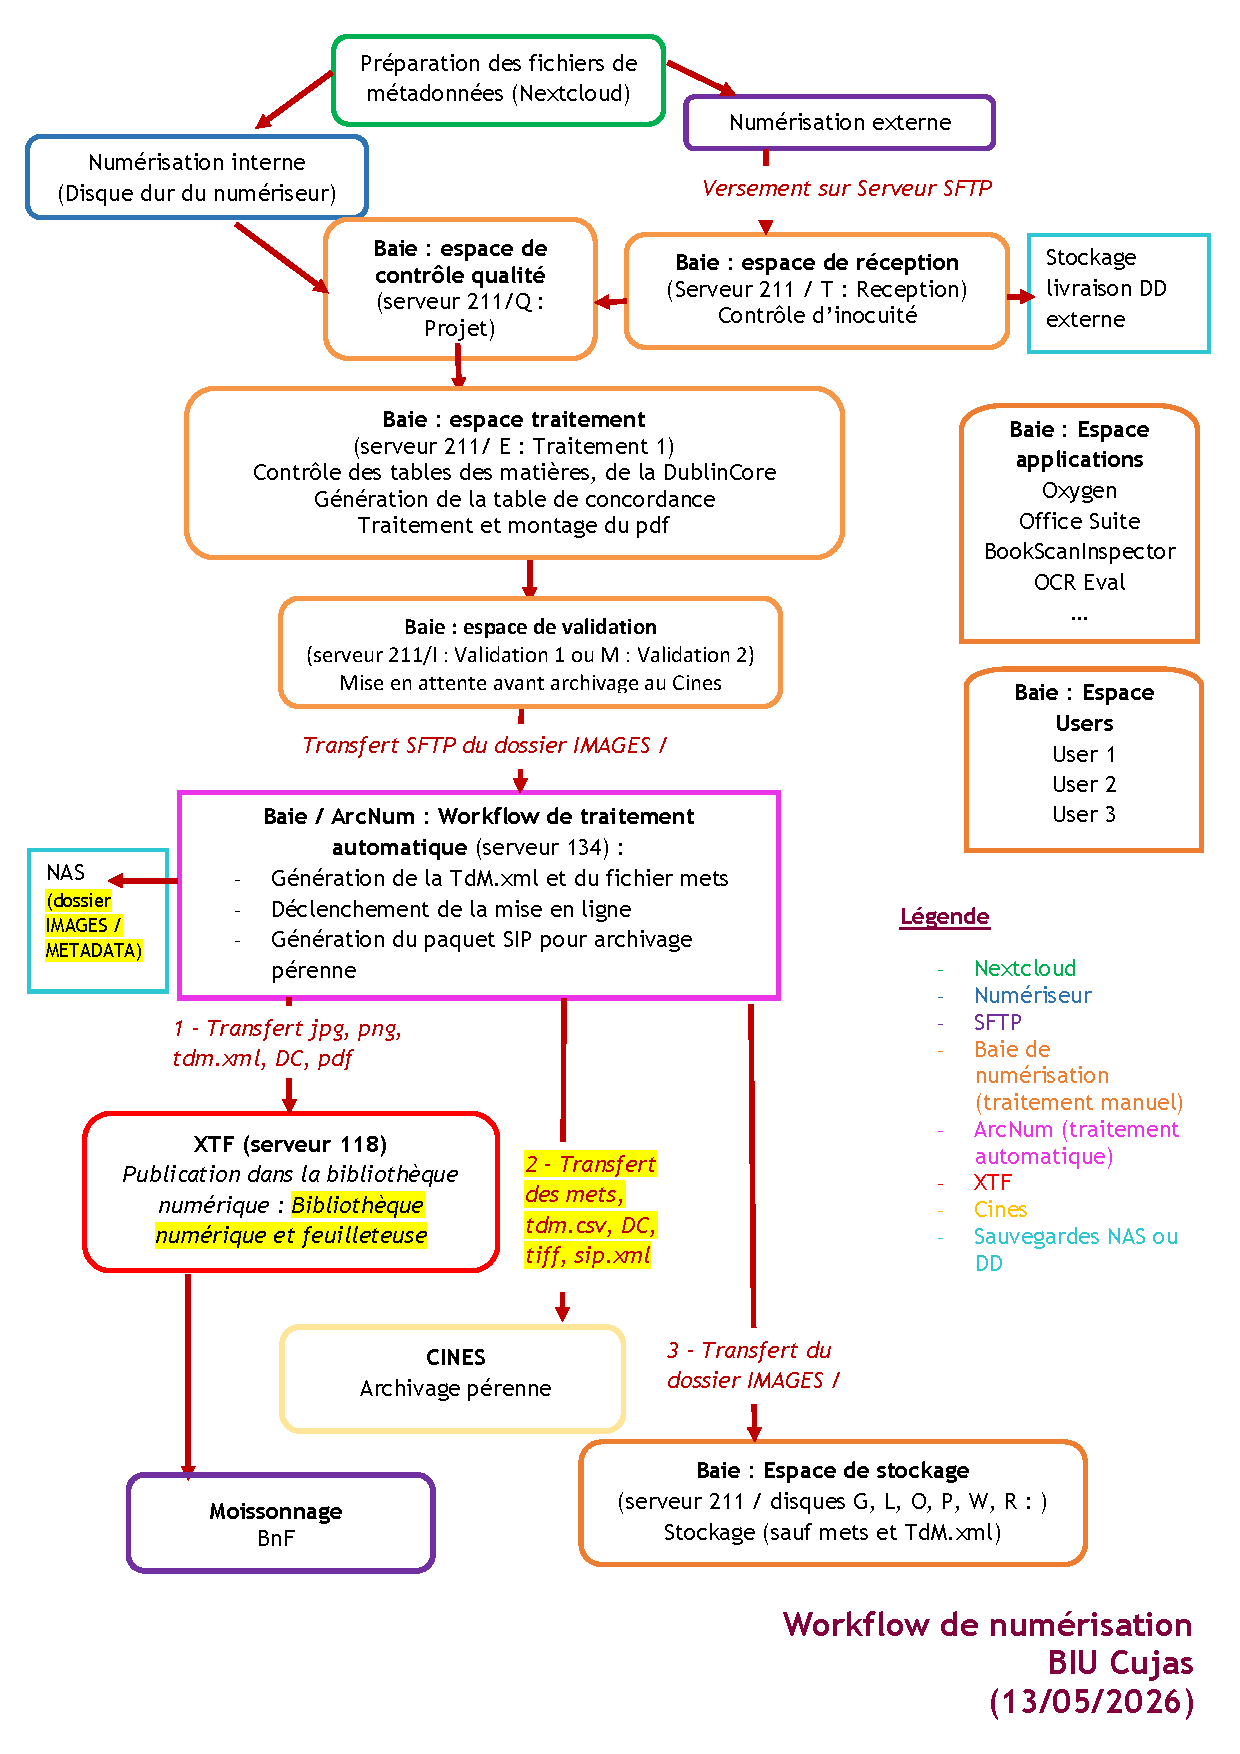
\includegraphics[width=0.5\linewidth]{202605_NUM_schemas_Workflow_prod_publ_V2.pdf}
		\caption{Schéma du workflow de production et de publication}
		\label{fig:workflow_prod_publ}
	\end{figure}

\subsection{Le matériel et le choix des chaînes de production (interne ou externe)}
La mise en œuvre concrète de cette chaîne de production a historiquement reposé sur l'acquisition d'un scanner de marque Kirtas à l'époque du projet Persée. Au-delà des arbitrages scientifiques, la mise en œuvre de la liste \enquote{Pfister-Roumy} se heurte rapidement aux contraintes matérielles de cet appareil. Cet équipement s'avère en effet beaucoup moins efficace que prévu, confrontant les agents à de \enquote{nombreux problèmes liés à son utilisation : il n'est pas possible d'utiliser toutes les fonctions automatiques de numérisation du scanner, forte probabilité de devoir passer en manuel pour les papiers anciens, difficultés de réglage et fréquents dysfonctionnements nécessitant d'éteindre et de rallumer les appareils et de refaire tous les réglages à chaque fois} \footcite{2007RefonteProgramme}. De surcroît, le scanner fait peser un fort risque de dégradation physique sur les documents originaux, dont la fragilité exige d'extrêmes précautions.

Malgré les difficultés logistiques pressenties face à l'ampleur d'un tel projet, l'établissement valide la liste \enquote{Pfister-Roumy} en articulant sa production autour d'une chaîne hybride. D'une part, à la suite de l'exposition virtuelle consacrée à Jean Carbonnier, la Bibliothèque Cujas dispose désormais d'une chaîne de numérisation en interne opérationnelle et prête à être mobilisée. Cette infrastructure s'est d'ailleurs renforcée grâce à la création de la célèbre \enquote{liste Pfister-Roumy}, une campagne de numérisation \enquote{alimentée entièrement en interne grâce aux compétences du département informatique} \footcite{2007RefonteProgramme}. Pour ce corpus, l'établissement fait le choix de traiter en interne exclusivement les \enquote{ouvrages postérieurs à 1830 avec l'océrisation et la relecture partielle sur les parties structurantes} \footcite{2007RefonteProgramme}. D'autre part, pour les documents antérieurs à 1830, la Bibliothèque Cujas privilégie une externalisation de la numérisation auprès d'un partenaire spécialisé, la société Puces et Plumes. Cette décision vise à \enquote{préserver le document}, car l'usage de son propre scanner représente un risque pour ces ouvrages déjà fragiles. Le prestataire se charge de numériser les documents en \enquote{mode image, [et] de faire la saisie fine des tables des matières} \footcite{2007RefonteProgramme}. Cette répartition stratégique du travail permet d'alimenter l'ambitieux projet de créer une bibliothèque numérique juridique fédérée unie par le protocole de moissonnage \ac{OAI-PMH}. Cette liste Pfister-Roumy constitue ainsi le véritable pilier fondateur de la bibliothèque numérique CujasNum.

Aujourd'hui, l'établissement dispose d'un nouveau matériel de numérisation de production récent (scanner de table de haute performance), ce qui permet de s'affranchir de ces contraintes historiques et de réévaluer la répartition entre traitements internes et externes. Le choix d'orienter un document vers la chaîne interne (numérisation sur place par les agents du \ac{DPCN}) ou vers une chaîne externe (prestataires ou chaînes de la \ac{BNF}) se fait désormais de manière stratégique par corpus, selon l'état de conservation physique de l'ouvrage, son format et les volumes à traiter.

\subsection{Le bordereau de numérisation}
Afin de garantir la bonne exécution de la campagne de numérisation, la méthodologie de travail de la Bibliothèque Cujas s'appuie sur l'établissement systématique d'un bordereau constituer de différentes parties. La première partie correspond à la notice bibliographique du document; la seconde détaille précisément sa pagination ainsi que les éventuelles particularités observées, par exemple des pages portant la même pagination; enfin, la dernière partie dresse l'état du document avant le transfert chez le prestataire \footannexe{\nameref{annexe_A_rapport_audit} pour voir l'entretien avec Sandrine Limandri qui détaille la façon dont la bibliothèque Cujas travail}.

\subsection{La phase de traitement: traitement d'images et OCRisation} 
Une fois la numérisation effectuée, la bibliothèque réceptionne les images brutes réalisées sous le format de conservation maître \ac{TIFF}. L'équipe effectue alors \enquote{un contrôle physique, livre en main, pour vérifier la complétude des images et s'assurer qu'aucune page ne manque par rapport au bordereau}\footannexe{\nameref{annexe_A_rapport_audit} pour voir l'entretien avec Sandrine Limandri.}. C'est par la suite qu'un script informatique local permet de générer les formats de diffusion légers (\ac{JPEG}, \ac{PDF}) et de produire automatiquement la table de concordance \enquote{qui fait correspondre chaque numéro d'image à la pagination réelle du livre}\footannexe{\ref{annexe_A_rapport_audit} pour voir l'entretien avec Sandrine Limandri.}. 

Cette orientation technique vers des fichiers statiques découle de la conception originelle de CujasNum, pensée comme \enquote{un simple répertoire \ac{PDF}} calqué sur la structure physique et matérielle d'un livre (volume et pages)\footannexe{\nameref{annexe_A_rapport_audit}.}. Pour dépasser cette contrainte et rendre la consultation des images plus ergonomique, une visionneuse \ac{JPEG} a été implémentée en 2013 pour permettre à l'usager de feuilleter le document de façon dynamique dans son navigateur\footannexe{\nameref{annexe_A_rapport_audit}.}.

\ac{XTF} possède de nombreuses contraintes techniques, l'une d'elles réside dans l'obligation d'avoir le format \ac{PDF} afin de mettre le document en ligne. Le système a été conçu comme \enquote{un simple répertoire \ac{PDF}} calqué sur la structure physique d'un livre (volume et pages)\footannexe{\nameref{annexe_A_rapport_audit}.}. Cela rend donc difficile l'ajout de tout autre types de documents ne respectant pas ce principe. Pour rendre la consultation des images plus agréable, une visionneuse \ac{JPEG} a été implémentée en 2013 pour permettre à l'usager de feuilleter le document de façon dynamique. 

Parallèlement au traitement de l'image, le traitement sémantique et textuel s'organise autour d'une stratégie d'océrisation (\ac{OCR}) différenciée. Au démarrage du traitement numérique, l'\ac{OCR} est appliqué exclusivement aux documents postérieurs à 1830 afin de permettre la recherche plein-texte au sein du texte imprimé\footcite{2011_programmeNumerisationPar}. Pour les ouvrages antérieurs à cette date charnière, la numérisation s'effectue uniquement en mode image pour préserver des supports physiques fragiles. L'absence d'\ac{OCR} sur le corpus de ces textes anciens est palliée par l'enrichissement sémantique de la table des matières, garantissant ainsi une navigation intellectuelle fine dans le document. Tandis que la personne en charge du contrôle qualité valide la conformité des métadonnées du Dublin Core, des moniteurs étudiants se voient confier la saisie intégrale de ces tables des matières sous format Excel/CSV, une tâche indispensable pour restituer fidèlement la structure de l'ouvrage et guider le chercheur\footannexe{\nameref{annexe_A_rapport_audit} pour voir l'entretien avec Sandrine Limandri.}.

\subsection{La phase de publication et d'archivage pérenne}
La validation définitive du contrôle qualité par l'équipe ouvre la voie à la phase finale de publication et d'archivage pérenne. Ce jalon requiert de minutieuses vérifications formelles et sémantiques effectuées par le technicien en charge de la validation. En plus de s'assurer de la conformité requise pour le versement au \ac{CINES}, le technicien doit \enquote{vérifier qu'il y a bien une image pour chaque page} et contrôler que le nommage de chaque fichier image respecte strictement la structure du \enquote{code-barres suivi du numéro d'image et de l'extension}\footannexe{\nameref{annexe_A_rapport_audit}.}. Il lui incombe également de s'assurer que les liens hypertextes figurant dans les métadonnées et commençant par le protocole non sécurisé \enquote{http} soient systématiquement remplacés par des adresses sécurisées \enquote{https} afin de prévenir tout blocage lors de l'ingestion ou de la consultation\footannexe{\nameref{annexe_A_rapport_audit}.}. 

Une fois ces critères formels validés, le protocole impose de contrôler la résolution et le taux de compression des images \ac{JPEG} et \ac{TIFF} à l'aide de l'outil \textit{IrfanView}, de verrouiller les fichiers \ac{PDF} de diffusion grâce à un mot de passe de protection institutionnel, et de valider la conformité de l'arborescence \ac{XML} du schéma de métadonnées Dublin Core afin de conjurer tout risque de rejet lors de l'ingestion par le \ac{CINES}\footcite{2010CRArchivage}. Les données sont ensuite transférées de manière asynchrone via un protocole \ac{SFTP} sécurisé (WinSCP) durant la nuit vers l'espace de publication final\footannexe{\nameref{annexe_A_rapport_audit} pour voir l'entretien avec Mebrouk Leulmi.}. Ce protocole de transfert différé, cloisonné et restreint a été mis en œuvre par le Département informatique technique (\ac{DIT}) à la suite d'une violente tentative d'attaque par rançongiciel subie par l'établissement en 2017, obligeant à sécuriser drastiquement tous les flux réseau entre la baie de traitement locale et les serveurs publics de l'université\footannexe{\nameref{annexe_A_rapport_audit} pour voir l'entretien avec Mebrouk Leulmi.}.

Le second volet de cette phase finale concerne l'archivage pérenne, confié au \ac{CINES}. Pour chaque ouvrage, la bibliothèque compile les fichiers d'images maîtres au format \ac{TIFF} et les fichiers de métadonnées descriptives et de gestion au format \ac{METS} (\textit{Metadata Encoding and Transmission Standard}) et PREMIS au sein d'un paquet de versement d'archives nommé \ac{SIP} (\textit{Submission Information Package})\footcite{2010CRArchivage}\footannexe{\nameref{annexe_A_rapport_audit} pour voir l'entretien avec Mebrouk Leulmi.}. Ce paquet standardisé garantit la préservation à long terme de la matière première numérique contre l'obsolescence matérielle. Néanmoins, ce circuit historique est aujourd'hui fragilisé. Le blocage récent des versements automatiques vers le \ac{CINES} contraint la Bibliothèque Cujas à conserver l'ensemble de ses fichiers intermédiaires au sein de son propre espace de stockage local (un \ac{NAS} de 40 à 50 téraoctets), provoquant une saturation critique de la baie de numérisation\footannexe{\nameref{annexe_A_rapport_audit}.}.

Cette procédure de versement réglementaire s'applique également aux documents dépourvus de structure linéaire, à l'instar du fonds iconographique de l'établissement. Pour répondre aux exigences d'ingestion du \ac{CINES}, les pièces d'images isolées doivent être compilées sous la forme d'un fichier \ac{PDF} unique. Le technicien élabore alors une table des matières et une table de concordance artificielles pour simuler la structure d'un volume physique, tandis qu'un plan d'archivage spécifique est défini conjointement avec les équipes du \ac{CINES} afin de valider ce profil de versement particulier\footannexe{\nameref{annexe_A_rapport_audit}.}.

Une autre particularité liée à la chaîne de numérisation réside dans l'indexation appliquée aux documents numériques de la bibliothèque numérique. C'est l'indexation Hauville qui est créée à partir de l'indexation \ac{RAMEAU}. 
\section{L’indexation propre à la bibliothèque Cujas}
La singularité de la Bibliothèque Cujas réside en grande partie dans l'adoption d'un système d'indexation tout à fait spécifique, peu utilisé et largement méconnu des autres établissements documentaires. La bibliothèque numérique s'appuie en effet sur cette indexation locale, une méthodologie originale qui doit son nom à sa conceptrice, qui a activement collaboré au projet de préfiguration de la première bibliothèque numérique de Cujas. 

Ce choix méthodologique s'explique par le fait qu'à sa création la bibliothèque numérique de Cujas reposait sur des \enquote{mots-clés libres qui généraient des incohérences} documentaires. Pour y remédier, il n'était cependant pas toujours envisageable de recourir au langage standardisé \ac{RAMEAU}, considéré comme inadapté au droit en raison de son caractère trop généraliste \footcite{cecilebolardLindexationPistePour2022}. C'est dans ce contexte que cette indexation a été développée : s'appuyant structurellement sur le référentiel \ac{RAMEAU}, elle ne le mobilise que lorsqu'il s'avère pertinent, mais n'hésite pas à le déconstruire dans le cas contraire afin de proposer des vedettes plus adaptées \footcite{2013_Num_Indexation_manuel_FHdocEspaceTravail}. 

Cette indexation débute par une phase d'analyse documentaire approfondie, au cours de laquelle le catalogueur examine le titre, la table des matières, et la quatrième de couverture, tout en procédant à l'identification des thèmes de l'ouvrage \footcite{2013_Num_Indexation_manuel_FHdocEspaceTravail}. Une fois ces concepts sémantiques identifiés, ils sont traduits dans le langage d'autorité national \ac{RAMEAU}. En l'absence de terme adéquat au sein de ce référentiel, l'établissement s'appuie \enquote{sur une forme normalisée qui est la plus courante comme Wikipédia ou vocabulaire des termes juridiques de Cornu par exemple} afin de combler les lacunes terminologiques du dictionnaire officiel \footcite{2013_Num_Indexation_manuel_FHdocEspaceTravail}. 

À l'issue de cette phase de normalisation, le technicien construit une vedette d'indexation structurée en deux ou trois éléments en fonction de la spécialité du domaine traité. Puis, il construit la vedette pouvant être composé entre deux ou trois éléments en fonction du domaine traité. Cette indexation comprend la vedette de forme (code, travaux préparatoires...), et le concept juridique. L'idée est de pouvoir \enquote{relire la vedette à l'envers en mettant un de ou dans le(s)} \footcite{2013_Num_Indexation_manuel_FHdocEspaceTravail}. Un exemple type de facette pouvant être trouvé sur CujasNum est celle-ci : Eglise -- Administration. Une autre particularité de cette indexation est la possibilité d'avoir \enquote{une indexation à la fois générique et spécifique. Il est possible d'avoir plusieurs vedettes construites ayant des liens de hiérarchie entre elles}, comme par exemple : Droit civil -- Obligations et Droit civil -- Contrats. Cela permet ainsi de mieux guider le lecteur \footcite{2013_Num_Indexation_manuel_FHdocEspaceTravail}.

À l'origine, l'application pratique de cette méthode d'indexation souffre d'un manque d'encadrement normatif au sein de la Bibliothèque Cujas. Il était en effet fréquent qu'elle soit faite par différente personnes, car il s'agissait initialement\enquote{de mots-clés apposés dans les notices Dublin Core}\footcite{2013_Num_Indexation_manuel_FHdocEspaceTravail}. La multiplication des personnes en charge de l'indexation ont rapidement entraîné\enquote{ainsi des incohérences} sémantiques majeures. Certains catalogueurs utilisaient par exemple un simple trait d'union tandis d'autres recouraient au tiret cadratin, une divergence typographique en apparence mineure mais suffisante pour générer artificiellement de nouvelles facettes redondantes et non connectées dans l'indexeur \ac{XTF} \footnote{\ref{annexe_A_rapport_audit}}. Pour pallier cette dérive et homogénéiser le catalogue, la direction impose un cadre strict en exigeant que \enquote{tout le monde indexerait de la même façon, en proposant de recourir à la liste d'autorité \ac{RAMEAU} sur BNOpale}\footcite{2013_Num_Indexation_manuel_FHdocEspaceTravail}.Face à ces difficultés structurelles, la \ac{BNF} recommande de \enquote{faire une liste fermée du vocabulaire utilisé \ac{RAMEAU} tant qu'il n'y a pas trop d'ouvrages numérisés}\footcite{2013_Num_Indexation_manuel_FHdocEspaceTravail}. Si l'astuce fonctionne ponctuellement, elle ne résiste pas au traitement de masse, la \ac{BNF} jugeant la méthode impraticable à l'échelle de plusieurs milliers d'unités. 

Bien que ce dispositif ait initialement été  validé par la \ac{BNF}, cette approbation s'est doublée d'une mise en garde prospective quant à sa pérennité. La \ac{BNF} soulignait en effet qu'un tel système d'autorités commencerait inévitablement à poser de sérieux problèmes de cohérence et de gestion documentaire dès lors que la bibliothèque numérique franchirait le seuil critique des 1 000 documents numérisés \footcite{2013_Num_Indexation_manuel_FHdocEspaceTravail}.

Clé de voûte d'une navigation fluide au sein d'une bibliothèque numérique, l'indexation repose entièrement sur la qualité des métadonnées -- décrites comme les \enquote{garants de fonctionnalités de recherche et de navigation satisfaisantes} \footcite{stutzmannSignalerRessourcesNumerisees2013}. Dès lors, l'interopérabilité des données s'avère cruciale : privée de cette capacité d'échange standardisé, une bibliothèque numérique risque son évincement progressif de la communauté malgré tous les services novateurs que celle-ci peut proposer. C'est précisément à l'aune de ce double impératif de description et d'interconnexion qu'il convient d'analyser les défaillances de l'infrastructure de CujasNum, dont l'obsolescence technique a progressivement transformé l'innovation initiale en une lourde dette technique.

\chapter[Le constat technique]{Le constat technique : l'innovation à la dette technique}

\lettrine{À} sa création, le choix de la solution logicielle destinée à supporter la bibliothèque numérique de Cujas s'est naturellement fondé sur l'état de l'art de l'époque. Les bibliothèques numériques étaient alors encore peu développées, ce qui limitait considérablement les options techniques pour les établissements désireux de concevoir de telles infrastructures. Le choix de Cujas s'est porté sur \ac{XTF}, une référence anglo-saxonne reconnue pour sa stabilité. Cette architecture logicielle répondait aux contraintes de l'époque, où ces plateformes se limitaient souvent à diffuser des \ac{PDF} volumineux dont le traitement exigeait une infrastructure solide.

Avec le temps, cette rigidité structurelle s'est toutefois transformé en un lourd fardeau technique pour l'établissement. la Bibliothèque Cujas s'est ainsi trouvée progressivement isolée en raison de l'impossibilité d'intégrer à l'architecture d'\ac{XTF} les nouveaux outils et standards du web de données. Aujourd'hui, CujasNum ne répond plus de manière satisfaisante aux attentes des usagers, ni à la vision moderne des bibliothèques numériques, désormais appréhendées comme de véritables vitrines institutionnelles indispensables pour garantir la visibilité et la découvrabilité des collections patrimoniales. Dès lors, il apparaît indispensable de faire évoluer cette infrastructure afin de mieux s'adapter aux usages actuels de la recherche et de rendre les métadonnées de CujasNum pleinement visibiles au sein du Web sémantique.

\section{Back-office : un effet \enquote{boîte noire}}
Si la bibliothèque numérique fait preuve de robustesse, sa limite majeure réside en coulisses: l'architecture du back-office. Face à un système fermé et dépourvu de documentation, les équipes métiers se retrouvent privées d'autonomie et de visibilité sur l'ensemble de la chaîne de traitement, ce qui entrave considérablement les cadences de production. 

Chaque tâche interne devient plus complexe notamment lorsque l'un d'eux repère une erreur syntaxique. Par exemple, ils peuvent la corriger mais ensuite ils doivent relancer toute la procédure de publication, ce qui prend du temps là, où une petite correction peut prendre entre une et deux minutes à être corrigée, et devrait être visible presque intantanément sur le portail de la bibliothèque \footannexe{\nameref{annexe_A_rapport_audit}.}. Ce n'est actuellement pas le cas pour la Bibliothèque Cujas qui se trouve contrainte de relancer son protocole de publication afin d'afficher l'erreur rectifiée. En effet, une fois l'erreur rectifiée, la personne en charge de la publication doit à nouveau rouvrir le \ac{PDF}, scellé par un mot de passe, modifier sa date de création, le verrouiller à nouveau, avant de le mettre en ligne\footannexe{\nameref{annexe_A_rapport_audit}.}. À chaque étape, ils doivent attendre que les traitements de nuit valident les étapes précédentes avant de pouvoir poursuivre les modifications, ajoutant une lourdeur à la procédure de travail \footannexe{\nameref{annexe_A_rapport_audit}.}. 

Le second problème vient de \ac{XTF} lui-même qui n'est plus maintenu. Habituellement, les inconvénients quotidiens ou difficultés rencontrées par les experts métiers étaient tous palliés par le responsable du \ac{DIT} \footannexe{\nameref{annexe_A_rapport_audit}.}. Toutefois, c'est loin d'être une bonne chose, car \enquote{tous les services de la bibliothèque numérique actuelle qu'ils soient interne ou externe reposent uniquement sur les compétences d'une seule et même personne}\footannexe{\nameref{annexe_A_rapport_audit}.}. Aujourd'hui, la bibliothèque numérique actuelle survit uniquement grâce aux compétences informatiques du responsable qui a su trouver des solutions comme l'ajout d'une visionneuse \ac{JPEG} permettant de consulter les ouvrages volumineux. 

Etant loin d'être un cas isolé, la situation de la Bibliothèque Cujas illustre bien la pensée de l'époque des institutions patrimoniales, ainsi que le concept du deuxième âge théorisé par Emmanuelle Bermès et Gautier Poupeau. Ce deuxième âge s'étend des années 1990 à 2010. Deux événements majeurs marquent cette période: l'irruption du Web au milieu des années 1990 et la numérisation de masse insufflée par Google à partir des années 2000 \footcite{bermesTroisAgesNumerique}. Cette époque correspond aux développements des projets de numérisation de la Bibliothèque Cujas qui s'est structurée selon les pratiques de travail de l'époque. Par ailleurs, c'est à ce moment-là qu'émerge les premières bibliothèques numériques \footcite{bermesTroisAgesNumerique}. 

Entre 1990 et 2010, les institutions patrimoniales ont une vision différente de la conception d'un document numérique. À l'épopque, les bibliothèques voient le document numérique comme une conversion du document physique. Jean-Michel Salaün théorise d'ailleurs cette idée qu'il définit \enquote{comme un ensemble de données organisées selon une structure fiable associées à des règles de mise en forme permettant une lisibilité partagée entre son concepteur et ses lecteurs} \footcite{pedauqueDocumentLumiereNumerique2006}. Avec l'émergence du web, de nouveaux standards se développent, utiles pour structurer les notices bibliographiques. C'est l'arrivée massif du format \ac{XML} qui permet le triomphe \enquote{de la pensée hiérarchique et documentaire}, modélisant les documents sous forme d'arborescences \footcite{bermesTroisAgesNumerique}. Le format \ac{XML} est alors pensé pour permettre la diffusion des données avec les autres bibliothèques sauf que l'arrivée des ordinateurs personnels freine paradoxalement l'innovation. Christine Ducourtieux l'exprime d'ailleurs ainsi : \enquote{l'arrivée des systèmes d'exploitation Windows et MacIntosh et de la bureautique ont paradoxalement pour effet de freiner l'élan d'innovation technique dans les méthodes, remplacé progressivement par des patriques discrètes : une appropriation de l'outil numérique plus individuelle, qui n'est plus subordonnée à l'histoire quantitative} \footcite{bermesTroisAgesNumerique}. Le développement de la technologie et l'arrivée de l'Internet en 1989, entraîne à nouveau une forme de cloisonnement avec un retour à l'individualisation des pratiques des chercheurs. 

En effet, l'arrivée des ordinateurs personnels bouleversent les pratiques créant une \enquote{séparation nette} entre l'édition scientifique et la numérisation de masse. Emmanuelle Bermès justifie cette hypothèse en expliquant que \enquote{l'édition scientifique numérique, qui reste le domaine de la recherche et peut s'adapter aux spécificités des corpus, et la numérisation, qui vise des masses documentaires plus importantes et traitées de manière homogène} \footcite{bermesTroisAgesNumerique}. Loin de favoriser la collaboration, cette évolution informatique tend à réisoler les pratiques de travail. Les bibliothèques numériques risquent alors d'être réduites à de simples entrepôts de fichiers \ac{PDF}, déconnectées des besoins de valorisation et du travail des chercheurs.

On observe aussi une parcellisation industrielle des tâches en bibliothèque. À cette époque, les tâches sont énormément segmentisées. Chaque personne a uniquement accès à ce qu'il doit faire, considérant qu'il n'est pas utile pour le bon déroulement de son travail d'avoir accès à l'intégralité du processus de production. La Bibliothèque Cujas est héritière de cette manière de travail mais c'est loin d'être un cas isolé car d'autres institutions patrimoniales comme la \ac{BNF} ont également rencontré ce problème. Michel Richard écrit sur ce sujet :\enquote{l'équipe responsable de la réalisation de ce programme comprend quinze personnes à plein temps rattachées sur le site d'Ivry. elle a en charge l'ensemble des tâches nécessaires à la constitution de la collection (travail bibliographique, contacts avec les universités et l'édition, relations avec la recherche, gestion du fonds électronique, commandes aux libraires, négocations avec les ayants droit, etc.) et au suivi de production (choix des prestataires, tests, contrôle qualité, gestion des stocks, normalisation, etc.)} \footcite{bermesTroisAgesNumerique}. Cela alourdit énormément le travail des bibliothécaires car c'est uniquement le \enquote{résultat final} qui est mutualisé et non le reste.  

La Bibliothèque Cujas fait d'ailleurs face à cette contrainte en disant clairement que le système actuel survit uniquement grâce aux compétences informatiques du responsable du \ac{DIT}. En dehors de lui, personne n'est à même à Cujas de pouvoir régler le problème entraînant ainsi une centralisation des compétences en une seule personne mettant en péril la pérennité de la bibliothèque numérique dans le futur. Les données deviennent alors vulnérables dans un monde où avec l'arrivée du Web sémantique, on réfléchit à ouvrir d'avantage les données afin de permettre une libre circulation de celle-ci.
\section{Vulnérabilité et sécurité des données}
À Cujas, le modèle de sécurité défensif se traduit par une infrastructure hermétique où des traitements \ac{SFTP} nocturnes dictent le rythme de production. Ce carcan technique isole les agents sur les postes de travail respectifs et fait obstacle à une véritable collaboration. En effet, la sécurité et la conservation étaient des priorités importantes dans le \enquote{deuxième âge du numérique} \footcite{bermesTroisAgesNumerique}. Avec l'explosion du web et la numérisation massive, cela multiplie le \enquote{potentiel numérique en matière de disponibilité des corpus} \footcite{bermesTroisAgesNumerique}. Face à cet essor, les institutions patrimoniales sont amenées à réfléchir à des moyens permettant l'ouverture de leurs données tout en les protégeant. Le \enquote{deuxième âge du numérique}, terme employé par Emmanuelle Bermès, illustre les enjeux de cette période notamment face aux \enquote{enjeux de structuration de l'information au format numérique, d'interopérabilité et de pérennisation} \footcite{bermesTroisAgesNumerique}. Cela permet aux institutions patrimoniales de mettre à disposition leurs contenus numérisés.

De plus, pour permettre cette diffusion du savoir, il est nécessaire d'utiliser les mêmes standards de structuration de la donnée, comme le MARC, utilisé pour rédiger les notices bibliographiques \footcite{westeelIndexerStructurerEchanger2010}. Aujourd'hui, ces règles permettent la transmission des documents numérisés entre les différentes bibliothèques numériques. Toutefois, ces concepts ont été mis en place d'une façon si stricte à la Bibliothèque Cujas qu'ils paralysent aujourd'hui le travail collaboratif des agents et figent les métadonnées. 

Cette posture d'hypervigilance s'enracine dans un incident marquant, révélateur des vulnérabilités locales de l'infrastructure. En 2017, la bibliothèque a en effet essuyé une attaque par rançongiciel: si cet assaut s'est soldé par la \enquote{perte de fichiers}, l'intervention du \ac{CINES} et la mobilisation de sauvegardes ont permis de préserver la majorité des images numériques. Le sinistre a néanmoins laissé des traces opérationnelles durables, contraingnant les équipes à reprendre intégralement le contrôle qualité et le traitement éditorial d'une cinquantaine d'ouvrages \footannexe{\nameref{annexe_A_rapport_audit}.}. La crainte de perdre à nouveau des données amène la Bibliothèque Cujas à se montrer davantage vigilante. Suite à cette attaque, \enquote{des sauvegardes journalières ont été mises en place de l'espace de traitement}. Cet événement illustre bien la fragilité des données \enquote{de traitement} par rapport aux données \enquote{d'archivage}\footannexe{\nameref{annexe_A_rapport_audit}.}. Ce traumatisme a eu pour effet de pousser l'informatique à verrouiller la chaîne de production au détriment de l'ergonomie. 

Cette sécurisation a entraîné un alourdissement de la chaîne de numérisation amenant à une saturation de leur \enquote{baie de numérisation}. En effet, la Bibliothèque Cujas utilise un espace de stockage local permettant de cloisonner les différentes étapes du processus de production. Chacun des espaces de stockage représente une tâche à effectuer. Cet espace de stockage est constitué de \ac{NAS}, possédant un espace de stockage massif entre 40 et 50 téraoctets \footannexe{\nameref{annexe_A_rapport_audit}.}. Aujourd'hui, cet espace est saturé, encombré de répertoires multiples qui rendent la structure globale illisible. Cette saturation résulte notamment du blocage lié à l'impossibilité temporaire de verser les fichiers \ac{SIP} au \ac{CINES}. La bibliothèque se trouve contrainte de les stocker dans son espace interne, l'amenant à repenser sa chaîne de numérisation \footannexe{\nameref{annexe_A_rapport_audit}.}. Elle envisage d'intégrer par exemple des formats d'images plus léger, comme le \ac{JPEG} ou JPEG 2 000 à l'instar des \ac{TIFF}, libérant ainsi de l'espace de stockage. De nombreuses bibliothèques patrimoniales, comme la Bibliothèque Sainte-Geneviève \ac{BSG} ou la Bibliothèque Sciences Po, ont également été confrontées à cette question. Elles ont choisi de faire ce basculement afin de libérer l'espace, tout en leur permettant de réduire leur empreinte carbonne liée à leur projet de numérisation \footcite{creusotQuellesPerspectivesPour}. Cela ne résoudrait que partiellement le problème, car qu'adviendrait-il des anciens versements. Devront-ils rester en l'état ? Pour l'instant la question demeure en suspens. 

Un autre des problèmes rencontré par la Bibliothèque Cujas, vient de la chaîne de numérisation elle-même. Le travail des experts métiers de la bibliothèque est extrêmement segmenté. Afin d'alléger légèrement leur travail, des moulinettes ont été crées, permettant une forme d'automatisation dans le travail des ouvrages numérisés \footannexe{\nameref{annexe_A_rapport_audit}.}. Ces moulinettes aident à combler des lacunes identifiées par le personnel qui a été mis en place par le responsable \ac{DIT} les soulageant par exemple dans la production des notices numériques. Cependant, le moindre changement peut entraîner une casse des \enquote{moulinettes} car correspondant à un schéma particulier de travail des équipes. Elles sont donc difficilement adaptable ou demandent une profonde réflexion afin d'améliorer au mieux la production \footannexe{\nameref{annexe_A_rapport_audit}.}. 

En réaction à l'attaque de 2017, le responsable du \ac{DIT} a énormément sécurisé les accès des équipes allant jusqu'à différencier les droits d'accès de chacun concernant les différentes étapes de production. Personne n'a accès à tous les paramètres. La publication des données ne peut plus se faire de façon simultanée car celles-ci passent désormais par un outil \ac{SFTP} sécurisé tels que WinSCP avec un traitement par lot \footannexe{\nameref{annexe_A_rapport_audit}.}. Ces transferts se réalisent uniquement la nuit, impactant nettement moins le travail des équipes selon le responsable du \ac{DIT}. En journée, l'espace est occupé ce qui ralentit davantage les traitements \footannexe{\nameref{annexe_A_rapport_audit}.}.

Le \ac{DPCN} travaille sur la baie de numérisation, uniquement accessible grâce aux codes d'accès sur des postes prédéfinis afin d'effectuer une tâche précise. Ayant été à l'origine comme un espace de stockage, il a fallu l'adapter pour permettre des connexions simultanées. Toutefois, des préccautions sont à prendre face à son instabilité, comme l'interdiction d'utiliser un moteur de recherche à l'intérieur afin de ne pas fragiliser l'infrastructure, et de protéger les données traitées \footannexe{\nameref{annexe_A_rapport_audit}.}. Par ailleurs, il est impossible pour les équipes de s'y connecter à distance que ce soit dans un autre lieu de la bibliothèque ou de chez eux. Le manque de structure suffisant de cette baie oblige à ce niveau prudence afin d'éviter la corruption des données.
 
Cette surprotection des équipes de Cujas via leur chaîne de numérisation amène à réfléchir à la notion même de sécurisation autour de la donnée. À une époque où l'on pense à ouvrir celle-ci à d'autres institutions patrimoniales afin de l'utiliser pour leur propre collection. Cette archive ouverte interroge sur le maintien des conditions de sécurité et de préservation nécessaire, sans complètement bloquer l'échange des métadonnées entre les institutions patrimoniales \footcite{bermesWebSemantiqueBibliotheque2013}. On observe une amplification de ce phénomène avec l'arrivée du Web sémantique. Bien sûr, la sécurité et la préservation sont des conditions nécessaires et importantes pour les bibliothèques mais ne doivent pas pour autant entraîner un isolement des données de l'institution à cause d'un modèle de sécurité trop stricte. Ce modèle de sécurité utilisé par Cujas est typique des silos du \enquote{deuxième âge}, créant une contradiction avec les méthodes de travail modernes empêchant une autonomie relative de la donnée \footcite{bermesTroisAgesNumerique}. 

Cette hypervigilance justifiée à bien des égards entraîne un isolement de la Bibliothèque Cujas par rapport aux autres bibliothèques numériques. La rigidité de ses conditions de travail entraîne comme conséquence l'impossibilité de faire évoluer son système pour répondre aux attentes d'aujourd'hui. Les exigences de maintenant sont davantage flexible avec le Web de données que dans les années 1990 et 2010 empêchant la bibliothèque d'améliorer l'ergonomie de son interface.
\section{L'impasse ergonomique}
Si l'infrastructure technique de CujasNum pose d'importants défis en termes de sécurité, la limite se révèle dans son fonctionnement quotidien. La chaîne de numérisation actuelle de la bibliothèque numérique illustre parfaitement l'approche décrite par Elina Leblanc dans sa thèse la qualifiant d'une \enquote{approche purement descendante(top-down), axée sur les contraintes du système plutôt que sur l'activité des agents} \footcite{leblancBibliothequesNumeriquesEnrichies}.

Elina Leblanc s'appuie sur les critères d'Aaron Schmidt, l'évaluation d'un service de bibliothèque numérique présente \enquote{un guide pour la CCU des bibliothèques analogiques [...]sous un angle utilisateur} \footcite{leblancBibliothequesNumeriquesEnrichies}. Il mentionne ainsi l'utilité d'un service d'une bibliothèque numérique en disant que celui-ci doit être \enquote{utilisable et désirable}. Aaron Schmidt l'explique ainsi : \enquote{Un service utile doit répondre à un besoin et avoir une importance aux yeux des utilisateurs pour qu'ils ne l'utilisent pas de manière ponctuelle, mais sur la longue durée. Un service utilisable garantit aux utilisateurs un accès aisé et rapide aux données. Enfin, la désirabilité crée un lien entre l'utilisateur et un service, en donnant envie au premier d'utiliser le deuxième et en suscitant un besoin} \footcite{leblancBibliothequesNumeriquesEnrichies}. Cela garantit à l'utilisateur une expérience optimale lorsqu'il utilise la bibliothèque numérique d'une institution patrimoniale. Or, à la Bibliothèque Cujas, l'interface n'est pas adaptée à la manière dont l'humain utilise les sites web aujourd'hui. L'utilisateur doit s'adapter aux contraintes rigides de l'interface et à la façon dont lui sont présentés les services. 

Ce manque d'ergonomie se traduit par un décalage dans la production des ouvrages numériques. Si le contrôle qualité d'un ouvrage requiert environ \enquote{quinze minutes en moyenne si tout va bien}, la moindre anomalie structurelle ou typographique fait basculer le traitement dans une autre dimension nécessitant au minimum \enquote{trois jours} de manipulations afin de corriger l'erreur détectée et ensuite pouvoir remettre en ligne le document \footannexe{\nameref{annexe_A_rapport_audit}.}. Cette manière de travailler est devenue un gouffre chronophage et la rigidité qu'implique ce traitement est devenue un carcan dont la Bibliothèque Cujas ne parvient pas à se défaire.

L'architecture d'\ac{XTF}, pensée pour les monographies, ne permet pas de l'adapter à d'autres types de documents avec des arborescences complexes, comme les périodiques. \ac{XTF} repose sur une arborescence dite \enquote{à plat}\footannexe{\nameref{annexe_A_rapport_audit}.}. C'est la raison pour laquelle si on ajoute d'autres types de documents l'arobrescence ne sera pas respectée, constituant un sérieux problème pour les équipes de Cujas qui souhaitent ajouter d'autres collections dans CujasNum.

Contrairement à une monographie, un périodique exige une architecture d'accès d'au moins trois niveaux, \enquote{c'est-à-dire le titre de la revue, suivie de l'année de publication et du numéro du volume ou du fascicule, pour que la consultation soit pertinente} \footannexe{\nameref{annexe_A_rapport_audit}.}. Etant incapable de reproduire cette structure, c'est l'une des raisons qui pousse la bibliothèque Cujas à mettre de côté ses collections ne pouvant les intégrer sans \enquote{dénaturer} le type de document. Aujourd'hui, on observe sur certaines bibliothèques numériques possédant des périodiques que la granularité peut aller jusqu'à l'article même. \ac{XTF} s'arrête initialement au volume et ne permet pas une granularité aussi précise, allant donc à l'encontre des pratiques de recherche actuelle. Faute de pouvoir diffuser ces revues dans sa bibliothèque numérique, Cujas a fait \enquote{le choix de faire numériser ces volumes via un partenariat avec Persée} \footannexe{\nameref{annexe_A_rapport_audit}.}. Pour signaler ces numérisations, la bibliothèque se contente uniquement de créer des notices de redirection indiquant aux chercheurs l'existance de ces documents, où il peut les trouver afin de les consulter. 

Un autre problème réside dans l'indexation utilisée par la bibliothèque numérique actuelle, l'indexation propre à la bibliothèque Cujas. Celle-ci ne permet pas le filtrage via différents types de documents; en effet elle a été structurée autour de la monographie ne permettant pas de croiser les informations \footcite{2013_Num_Indexation_manuel_FHdocEspaceTravail}. L'impossibilité d'ajouter d'autres types de documents met en lumière l'invisibilisation à laquelle on se trouve confronté lors d'une recherche plein-texte. Ces documents ne peuvent ressortir de manière évidente ne pouvant posséder d'\ac{OCR}. Les résultats apparaissent donc de façon très restreinte et dans les dernières pages problablement \footannexe{\nameref{annexe_A_rapport_audit}.}. L'obsolescence du logiciel \ac{XTF} entraîne donc \textit{de facto} un filtrage empêchant la Bibliothèque Cujas de pouvoir mettre en avant la richesse et la diversité de ses collections. Il lui est impossible de valoriser ses documents afin de justifier les choix effectués ou de mettre en avant une collection ou un document dans un article ou dans une exposition virtuelle. 
\medskip

Le bilan de CujasNum met en avant les points forts du projet ainsi que les points faibles au moment de la réalisation de celui-ci, mais également ceux ayant émergé par la suite avec l'évolution des technoloqies numériques et des pratiques du Web. D'abord, pionnière dans le monde des bibliothèques numériques, la Bibliothèque Cujas s'est trouvée progressivement isolée, parvenant difficilement à suivre l'évolution rapide liée à l'émergence de l'internet entraînant les pratiques documentaires et les pratiques d'Internet dans un nouvel âge. Face à ce constat, \enquote{l'ajout d'une surcouche WordPress ne s'aurait être la solution comme cela avait été envisagé dans un premier temps} \footannexe{\nameref{annexe_A_rapport_audit}.}. Pour répondre aux attentes contemporaines des chercheurs et pour s'adapter aux mutations nationales, des systèmes de gestion des bibliothèques (SGB) imposent une rupture dans les pratiques actuelles. Cela nécessite de réfléchir à une interface plus souple, acceptant différents types de documents se basant sur les pratiques actuelles de la recherche, répondant aux nouveaux enjeux des utilisateurs. La bibliothèque numérique doit permettre à sa bibliothèque d'utiliser les standards du Web de données afin de rendre sa plateforme davantage interopérable et prête à s'intégrer dans de grands réseaux scientifiques nationaux.

%%%%%%%%%%%%%%%%% CONCLUSION DE LA PARTIE I %%%%%%%%%%%%%%%%%%%%

\section*{Conclusion de la Première Partie}
\lettrine{C}et état des lieux éclaire la trajectoire singulière de la Bibliothèque interuniversitaire Cujas, pôle national de référence pour la recherche juridique, et dresse un bilan critique de sa première vitrine numérique, CujasNum. Si l'établissement a été pionnière au début des années 2000 en numérisant des corpus scientifiques d'exception — à l'instar des cours polycopiés du doyen Jean Carbonnier et de la célèbre \enquote{liste Pfister-Roumy} de sources doctrinales —, cette dynamique de valorisation se heurte aujourd'hui aux limites de ses choix technologiques d'origine.
Le choix du framework \ac{XTF}, jugé à l'époque optimal pour sa robustesse matérielle, s'est progressivement transformé en un carcan technique. Son architecture de données \enquote{à plat} condamne la plateforme à ne diffuser que des monographies, invisibilisant de fait les collections de périodiques ou d'archives dont la structure hiérarchique complexe ne peut y être modélisée. Au quotidien, cette rigidité logicielle impose aux experts métiers une chaîne de production segmentée et opaque, assimilée à une \enquote{boîte noire}. La retranscription manuelle des tables des matières sous tableur, l'attention constante portée aux moindres anomalies de balisage \ac{XML} pour répondre aux exigences du \ac{CINES}, et la lourdeur des corrections in situ s'apparentent à un \enquote{bricolage permanent} qui pèse lourdement sur le temps de travail des agents.
Cette pénibilité opérationnelle s'est trouvée renforcée par une stratégie de sécurisation purement défensive. Marqué par le traumatisme de la cyberattaque par rançongiciel subie en 2017, l'établissement a fait le choix d'un cloisonnement technique strict : serveurs fermés, interdiction de connexion à distance pour les équipes de production, et transferts \ac{SFTP} nocturnes différés. Bien que légitime, cette hypervigilance paralyse le travail collaboratif et fige les métadonnées.
Enfin, l'impasse est également ergonomique et documentaire. Aujourd'hui CujasNum est axée sur les contraintes du système, et n'est plus adaptée aux pratiques de recherche contemporaines. Cet éloignement s'explique notamment à cause d'un PageRank médiocre sur les moteurs de recherche, et l'absence d'un espace de travail personnel et persistant dédié aux chercheurs.
Le bilan de CujasNum démontre qu'une simple mise à jour ou l'ajout d'une surcouche applicative comme WordPress ne sauraient résoudre cette dette technique accumulée. Pour asseoir à nouveau sa légitimité de pôle de référence sémantique, la \ac{BIU Cujas} doit opérer une rupture franche. Il est désormais indispensable de dépasser le modèle du simple \enquote{répertoire de PDF} fermé pour faire entrer l'établissement dans le troisième âge du numérique. Cette transition, qui impose d'ouvrir les données, de les modéliser en graphes de triplets \ac{RDF} interopérables et d'adopter des standards universels (IIIF, IFLA-LRM).

%%%%%%%%%%%%%%%%%%%%%%%%% Partie II %%%%%%%%%%%%%%%%%%%%%%%%%%
%%%%%%%%%%%%%%%%%%%%%%%%%%%%%%%%%%%%%%%%%%%%%%%%%%%%%%%%%%%%%%

	\part{De la théorie à la pratique : évaluer les besoins au sein des réseaux documentaires interconnectés}
	
%%%%%%%%%%%%%%%%%%%%%%%%%% INTRODUCTION %%%%%%%%%%%%%%%%%%%%%%%%%%

\begin{quote}
	\enquote{La bibliothèque numérique dispose d'atouts pour répondre aux usages actuels du web:
	\begin{itemize}
		\item des métadonnées descriptives, dont la fiabilité est assurée par les normes de standards des bibliothèques: celles-ci permettent aux usagers d'accorder leur confiance aux contenus et favorisent le référencement et l'interopérabilité de la ;
		\item des contenus (livres, images, sons, etc.) consultables en ligne, parfois même téléchargeables et réutilisables.
		\end{itemize}} \footcite{claerrManuelConstitutionBibliotheques2013a}.
\end{quote}

\lettrine{U}ne bibliothèque numérique peut détenir tous les atouts possibles ; il reste néanmoins primordial que celle-ci permette à l'usager de trouver les documents, les sélectionner et les utiliser selon ses besoins. Face à la surabondance informationnelle, les bibliothèques doivent redoubler de stratégie afin d'apporter une meilleure visibilité à leur contenu leur permettant ainsi de se trouver sur le \enquote{chemin de l'usager}. Pauline Moirez et Dominique Stutzmann insistent sur l'idée de ne pas concevoir la bibliothèque numérique comme un \enquote{lieu unique et fermé}. Ils recommandent de s'interroger sur l'architecture de gestion, les bénéfices d'un enrichissement de métadonnées, l'échange de données \footcite{claerrManuelConstitutionBibliotheques2013a}. Ces atouts amènent à transformer la manière dont travaillent les bibliothécaires.

Le passage de la bibliothèque numérique CujasNum d'un modèle de production en silo fermé à un écosystème de catalogage partagé ne se réduit pas à une simple mise à niveau technique, mais consacre un profond changement de paradigme documentaire. Cette deuxième partie explore la manière dont les métadonnées s'affranchissent de leurs limites locales pour s'intégrer nativement dans le Web de données. L'articulation de nos chapitres démontre comment les principes fondamentaux du Web sémantique — à l'instar du modèle \ac{RDF}, de sa structuration en triplets (sujet, prédicat, objet) et du recours systématique aux identifiants pérennes (\ac{URI}, \ac{ARK}) — permettent de transformer des notices statiques en ressources dynamiques et interconnectées. Au cœur de cette architecture, l'adoption du modèle conceptuel \ac{IFLA-LRM} et l'alignement d'autorités locales spécifiques, comme l'indexation juridique Hauville, avec des référentiels nationaux d'autorité tels que \ac{RAMEAU} et IdRef, constituent la clé de voûte de la future plateforme Codex. C'est par cette déconstruction de la notice traditionnelle que la donnée acquiert son autonomie, garantissant l'interopérabilité et la visibilité des collections de la Bibliothèque Cujas sur le Web sémantique.

%%%%%%%%%%%%%%%%%%%%%%%%%% CHAPITRE %%%%%%%%%%%%%%%%%%%%%%%%%%%%%%

\chapter[Les attentes internes]{Les attentes internes: inscrire Cujas dans une stratégie nationale}

\lettrine{L}'ère des bibliothèques numériques isolées, conçues comme de simples \enquote{répertoire de \ac{PDF}} ou de données isolées les unes des autres est maintenant révolue. L'essor de la Science Ouverte et la nécessité de valoriser la recherche publique, imposent désormais de nouvelles exigences de découvrabilité ainsi qu'une refonte des infrastructuress documentaires. Le constat technique effecuté sur CujasNum, marqué par l'obsolescence de son logiciel \ac{XTF}, l'impossibilité d'un moissonnage \ac{OAI-PMH} par Gallica et la vulnérabilité d'un système reposant sur une compétence humaine unique, met en exergue son dysfonctionnement matériel. Loin d'être isolé, il témoigne des limites structurelles du deuxième âge du numérique, caractérisé par une interopérabilité \enquote{par copie et conversion} de notices plates ou de pertes de données en passant du format MARC au Dublin Core, et est devenu inapte à exprimer la richesse sémantique des collections des institutions patrimoniales \footcite{bermesTroisAgesNumerique}. Face à ce constat la \ac{BIU Cujas} a choisi d'inscrire la refonte de sa bibliothèque numérique dans une stratégie nationale. Cette refonte a pour objectif de s'inspirer du Web de données afin de s'appuyer sur les réseaux de bibliothèques numériques et de valoriser ainsi ses nombreuses collections.

\section{Du silo local au catalogage partagé}
La refonte de la bibliothèque numérique amène actuellement la \ac{BIU Cujas} a réfléchir à la manière dont celle-ci travaille. Cette refonte entraîne également une refonte de la chaîne de numérisation, fonctionnant principalement de façon isolée et manuelle. Le \ac{DPCN} cherche un moyen de sortir de ce carcan afin de pouvoir automatiser d'avantage de tâches en minimisant l'impact humain. Bien sûr, il est important de ne pas supprimer complètement la supervision humaine, et de réfléchir à un moyen d'enrayer un travail devenu, avec le temps, chronophage.

\subsection{Les limites du catalogage en silo et la dérive des notices déconnectées}

Actuellement, la création des métadonnées sous CujasNum repose sur une production segmentée des tâches: le prestataire saisit les métadonnées dans la Dublin Core en s'appuyant sur le bordereau fourni au moment de la livraison par la bibliothèque. Une fois, la numérisation effectuée, le technicien, en charge du contrôle qualité, ouvre la Dublin Core et effectue des micro-corrections lorsque cela est nécessaire. Il fait attention à ce que le schéma soit bien déclaré, que ce soit les bons guillemets \footannexe{\nameref{annexe_A_rapport_audit}.}. 

Historiquement, avant 2013, la Bibliothèque Cujas ne disposait d'aucun agent formé au catalogage du livre ancien \footannexe{\nameref{annexe_A_rapport_audit}.}. Il n'existait pas à cette époque de standardisation afin d'indiquer comment la notice devait être construite. La logique était d'utiliser, lorsqu'elle existait, la notice cataloguée en ligne. Quand il n'y avait pas de modèle existant, la personne chargée de ce catalogage descendait dans le magasin pour décrire la notice à partir de l'ouvrage papier en renseignant autant d'information qu'il lui était possible de le faire \footannexe{\nameref{annexe_A_rapport_audit}.}. Cette manière de procéder crée des notices numériques inégales. Certaines étaient riches et d'autres extrêmement pauvres ou incomplètes, demandant aujourd'hui une reprise complète avant de pouvoir envisager le moindre enrichissement de notices.

En effet, pour éviter de créer des notices bibliographiques déjà existantes, il est nécessaire, pour les bibliothèques, de sortir de leur production en silo correspondant au \enquote{stockage de l'information dans une base locale, isolée, dont le catalogue traditionnel est l'archétype} \footcite{bernonLierBasesLocales2017}. Le Web de données a pour but de \enquote{sortir l'information de ces silos} pour la rendre exploitable, de manière distribuée \footcite{bermesWebSemantiqueBibliotheque2013}. L'enrichissiment des notices est possible grâce au web sémantique qui \enquote{permet d'exposer des données, des contenus d'une manière beaucoup plus riche qu'à l'heure actuelle, et permet d'encourager des collaborations transdisciplinaires et le croisement entre professions de la culture ou de la recherche} \footcite{melhemUsagesApplicationsWeb}. 

Pour permettre ces enrichissements, de nombreuses institutions patrimoniales ont effectué des chantiers de nettoyage de notices afin de permettre des alignements sur des référentiels d'autorité comme IdRef \footcite{nicolasAtomesCrochusMetadonnees2016}. Cette étape, jugée primordiale permet d'avoir des notices propres et enrichies, participe à la visibilité de la bibliothèque numérique par les autres institutions et permet ainsi à celle-ci de pouvoir créer des rebonds en s'appuyant sur ce référentiel. 

En 2023, la Bibliothèque Cujas faisait face au problème de déconnexion entre le catalogage et le traitement numérique. Lors de la création des notices bibliographiques, deux méthodes se chevauchent: soit les agents créent la notice de toute pièce soit ils se contentent d'un lien cliquable. Il est nécessaire de résoudre ce problème qui impacte sérieusement le reste de la chaîne de numérisation\footannexe{\nameref{annexe_A_rapport_audit}.} . En effet, \enquote{le catalogage des documents numérisés doit être effectué en début de chaîne : tout retard impacte l'ensemble des opérations qui suivent}. Un autre problème vient de la politique de catalogage elle-même, qui, comme nous l'avons vu, n'est pas \enquote{bien définie : parfois une notice de document électronique a été créée, parfois un lien vers CujasNum a été ajouté dans le champs Unimarc 856} \footannexe{\nameref{annexe_A_rapport_audit}.}. Le moissonnage de ces notices étant imparfait, la notice créée pour CujasNum est celle se retrouvant dans le catalogue de la bibliothèque. Face à ces problèmes répétés, la bibliothèque a pris énormément de retard dans son catalogage et son indexation. En effet, on peut le voir avec les cours polycopiés \enquote{numérisés en 2020 qui n'ont pas été catalogués.}\footannexe{\nameref{annexe_A_rapport_audit}.}. Un travail rétrospectif est nécessaire une fois que les notices ont été modifiées, de \enquote{modifier rétrospectivement les métadonnées en Dublin Core} \footannexe{\nameref{annexe_A_rapport_audit}.}. Ces inconvénients créent des retards voir des doublons dans l'outil de découverte Primo. 

La majorité des bibliothèques utilise le Dublin Core simple, constitué de 15 balises mais la plupart des bibliothèques n'en utilise réellement que cinq (creator, identifeir, title, date, type). En effet, cela comprend \enquote{74 \% des fournisseurs qui ne dépassaient pas l'utilisation de cinq éléments} \footcite{lavennedelamontoiseOAIPMHPMHLheure2020}. L'adoption massive de ce format par les institutions patrimoniales comme les bibliothèques a entraîné un appauvrissement des données contrairement aux données que celles-ci pouvaient encoder au format MARC. L'appauvrissement constaté des notices bibliographiques résulte paradoxalement de la volonté des bibliothèques de rendre leurs données interopérables et visibles sur le Web. Face à la diversité et à la complexité des formats d'encodage (tels que le format MARC utilisé dans des systèmes comme Alma), l'interopérabilité directe s'avère difficile à mettre en oeuvre. Les institutions patrimoniales ont donc recours au Dublin Core simple, un standard minimaliste adopté comme \enquote{le plus petit commun dénominateur} \footcite{lavennedelamontoiseOAIPMHPMHLheure2020}. Couplé au protocole \ac{OAI-PMH} pour le moissonnage automatisé, ce format pivot permet une diffusion immédiate, universelle et à bas coût des données sur le Web, au prix d'une simplification transitoire de l'information bibliographique. En effet, les universités possédant peu de moyens doivent trouver des alternatives à bas coût permettant leur exposition sur le web de données. C'est ainsi que l'idée induite par l'utilisation de ce format est \enquote{de favoriser la création d'archives ouvertes institutionnelles, et de créer un réseau pour les fédérer, et en même temps participer à améliorer la qualité des métadonnées échangées}. Le protocole \ac{OAI-PMH} assure cet \enquote{échange de métadonnées, à un moment où l'inflation de contenus sur le Web} explose \footcite{lavennedelamontoiseOAIPMHPMHLheure2020}. C'est également une plus-value pour les chercheurs car cela permet de présenter les informations bibliographiques de la même manière ne perturbant nullement l'utilisateur lorsqu'il consulte plusieurs bibliothèques numériques différentes. 

Toutefois, cette simplification transitoire s'est fait au détriment de la richesse des données. Comme le rappelle une responsable de bibliothèque numérique, le signalement devrait être pensé comme un véritable \enquote{passport du document} exigeant une description exhaustive (aspects physiques, particularités d'exemplaires) essentielle pour les chercheurs \footannexe{\nameref{annexe_A_rapport_audit}.}. De surcroît, cette logique de diffusion est paralysée pour la Bibliothèque Cujas : l'entrepôt \ac{OAI-PMH} de CujasNum, basé sur une version d'\ac{XTF} non mise à jour, est devenu impossible à moissonner par les partenataires nationaux, comme la \ac{BNF}, l'enfermant dans un véritable silo technique. 

Les équipes de Cujas espèrent qu'avec la refonte de leur bibliothèque numérique, les problèmes de moissonnage et de constitutions de notices soient rectifiés afin d'avoir une meilleure visibilité sur le web. 

\subsection{Les exigences internes pour la refonte}
Il est primordial pour les agents de Cujas de parvenir à intégrer leurs notices bibliographiques dans le catalogue \ac{SUDOC}, ce qui n'est pas le cas pour le moment. En intégrant ce catalogue, cela leur permet ainsi de mieux signaler leurs collections de la même manière que le font les autres bibliothèques. 

La majorité des bibliothèques se sont mises à \enquote{rationaliser la production des données} afin de profiter de ce qu'offre le Web de données aux bibliothèques. Il offre l'opportunité de répartir l'activité de description de leurs fonds de manière décentralisée, \enquote{différents acteurs enrichissant le même graphe} \footcite{bermesWebSemantiqueBibliotheque2013}. Cela justifie la proposition de la Bibliothèque Cujas de \enquote{traiter le catalogage et l'indexation sémantique en amont dans  le \ac{SUDOC}} pour que la notice \enquote{bavarde} redescende proprement dans Alma et le prototype, plutôt que de devoir la corriger à la main au moment du contrôle qualité \footannexe{\nameref{annexe_A_rapport_audit}.}. Cette proposition formulée par le Département de l'information documentaire \ac{DID} et le \ac{DPCN} est \enquote{d'abandonner la double saisie locale}, entraînant sans arrêt le retour en arrière sur une tâche en ayant l'impression qu'elle n'aboutit jamais ou plus tardivement que le souhait initial \footannexe{\nameref{annexe_A_rapport_audit}.}. Il faudrait que dans le futur le prototype puisse s'interconnecter nativement avec le \ac{SUDOC} pour récupérer des notices propres et éviter les doublons. 

Une autre des volontés des experts métiers est d'avoir accès à un back-office structuré où à l'intérieur sont prédéfinis des rôles pour chaque profil (catalogueur, éditeur, responsable). Cela permettrait d'avoir une infrastructure balise où les droits d'accès sont délimités à l'avance en fonction des tâches assignées à un agent sans mettre en péril le reste de la production si une nouvelle connexion d'un autre agent venant destabiliser la structure \footannexe{\nameref{annexe_A_rapport_audit}.}. Les profils permettraient ainsi au responsable de la bibliothèque numérique de pouvoir assigner aux utilisateurs des rôles avec des tâches dédiées. Par exemple, si une personne est en charge de l'éditorialisation, alors elle aura accès uniquement aux parties lui permettant de mener à bien sa mission. Cela aurait comme conséquence de décentraliser le travail et de ne plus être dépendant des compétences du responsable informatique. La bibliothèque aimerait que le back-office soit \enquote{administrable par un bibliothécaire}, suffisamment balisé et facile à prendre en main afin d'en décharger le responsable du \ac{DIT} et de lui permettre de se concentrer sur le maintien technique et mises à jour de la bibliothèque; les experts métiers gérants totalement la partie production, mise en ligne et correction des micro-erreurs typographiques \footannexe{\nameref{annexe_A_rapport_audit}.}. 

Ce n'est pas la seule exigence interne des agents en charge de la bibliothèque car avant de mettre en place ces droits, il est tout aussi important de s'occuper de leurs métadonnées. Cela représente un chantier important à réaliser en priorité pour la bibliothèque. Cujas est loin d'être la seule bibliohèque patrimoniale à avoir rencontré ce problème lié aux métadonnées \footannexe{\nameref{annexe_A_rapport_audit}.}. En effet, toutes les institutions patrimoniales ayant souhaité une refonte de leur bibliothèque numérique sont passées par cette étape jugée comme importante par des experts en charge de bibliothèques numériques. L'un d'entre eux insiste en décrivant cette \enquote{étape comme étant indispensable} pour lier de nombreuses notices en ayant recours à OpenRefine permettant un alignement des notices bibliographiques au référentiel d'IdRef. \footannexe{\nameref{annexe_A_rapport_audit}.}. Un autre responsable mentionne également l'importance de nettoyer ces notices car \enquote{si on ne les nettoie pas, cela crée énormément de bruit, créant ainsi des résultats insuffisants}, alors que lorsqu'elles \enquote{sont normés et standardisée, cela ne représente pas un problème}\footannexe{\nameref{annexe_A_rapport_audit}.}. 

Cette refonte s'avère indispensable pour corriger les dysfonctionnements observés sur CujasNum. L'alignement sur des protocoles standardisés constitue un gage de fiabilité qui permet, selon les équipes, de prévenir nombre d'anomalies techniques récurrentes. Il convient de prêter attention aux notices récentes mais aussi aux plus anciennes. En effet, comme expliqué en amont, les notices bibliographiques de livres anciens, pour la plupart, peuvent être pauvres car il n'existait pas avant les années 2010 de format de standardisation propre pour ce type d'ouvrage.

Les alignements permettent d'intégrer les notices bibliographiques dans le Web de données amenant une meilleure visibilité de celles-ci sur Internet et permettant aux bibliothèques de lutter contre \enquote{l'info-obésité} à laquelle sont confrontés quotidiennement les usagers. 
\section{Le Web de données et les nouveaux protocoles}
Auparavant, la diffusion des données était davantage passive. Les bibliothèques numériques interrogeaient les entrepôts OAI afin de moisssonner leurs métadonnées, sans forcément interagir directement avec celles-ci. La transition de la bibliothèque numérique de la \ac{BIU Cujas} vers le Web sémantique ne saurait être réduite à une simple mise à jour d'infrastructure : elle engage une véritable refondation de l'objet documentaire lui-même. Aujourd'hui, le document numérique rompt définitivement avec la logique de faire la numérisation sous forme de captures d'image. Désormais, la représentation du document numérisé est devenue plus complexe. Comme l'a théorisé Jean-Michel Salaün au sein du collectif Roger T. Pédauque, \enquote{il est probable que le document numérique donne une dimension nouvelle à la notion d’intertextualité. Celle-ci se prolonge dans l’inter-sémioticité. L’inter-sémioticité du document numérique qui intègre texte, écrit, image et son ne change pas la nature du texte, elle en accroît en revanche la complexité. Les rapports d’inclusion réciproque constituent un objet de recherche nouveau qui devrait mieux spécifier la relation entre sémantique et sémiotique} \footcite{pedauqueDocumentLumiereNumerique2006}. Le document numérique est devenu un objet structuré en trois dimension : à travers la forme, le texte et l'interconnexion sémantique. C'est pourquoi, faire entrer le patrimoine juridique dans le Web de données (Linked Open Data) consiste à matérialiser cette déconstruction pour substituer au document-objet traditionnel un objet dynamique et ouvert d'entités liées.

\subsubsection{La rigueur de la structure logique}
La structure logique des documents numérisés constitue le fondement de toute bibliothèque numérique patrimoniale. Comme le rappelle Isabelle Westeel, à partir des années 1970, l'émergence historique des langages de balises vient \enquote{de la nécessité de structurer l'information}, en se préoccupant \enquote{du contenu du document et non pas de sa mise en forme (contrairement au \ac{HTML} qui gère des balises de mise en forme)} \footcite{westeelIndexerStructurerEchanger2010}. Cette évolution consacre une distinction majeure dans la composition du document entre \enquote{une structure logique (contenu organisé) et d'une structure physique (mise en forme de l'information)} \footcite{westeelIndexerStructurerEchanger2010}. Toutefois, la simple conformité syntaxique n'est pas suffisante pour garantir l'interopérabilité des données. Le document est \enquote{bien formé}, lorsqu'il respecte \enquote{l'ensemble des règles de la recommandation} ou l'utilisation de la DTD \textit{Document Type Definition} et des schémas \ac{XML}. La DTD liste les éléments, les attributs associés dans le document, participant l'interopérabilité des métadonnées \footcite{westeelIndexerStructurerEchanger2010}.

Ce sont ces mêmes métadonnées qui sont moissonnées à travers les entrepôts d'\ac{OAI-PMH} des bibliothèques. Actuellement, l'entrepôt d'\ac{OAI-PMH} de CujasNum rencontre des problèmes de moissonnage. L'une des raisons vient de l'absence de balises obligatoires comme \enquote{earliestDatestamp}, bloquant le moissonnage automatique par Gallica. Face à ce problème récurrant auquel est confronté la Bibliothèque Cujas, l'établisssement souhaite qu'avec la nouvelle bibliothèque le moissonnage se fasse de nouveau. En effet, de l'impossibilité de faire moissonner leurs collections par les institutions nationales, comme la \ac{BNF}, il résulte un manque de visibilité de leurs documents dans le Web de données.

\subsection{Le dépassement de l'OAI-PMH : de la diffusion passive aux données liées}
Depuis les années 2000, le protocole \ac{OAI-PMH}, couplé au format Dublin Core simple a constitué la brique standard incontournable pour le moissonnage des métadonnées sur le Web \footcite{lavennedelamontoiseOAIPMHPMHLheure2020}. Si cette simplification transitoire a permis une diffusion à bas coût de l'information bibliographique, elle se heurte aujourd'hui aux exigences scientifiques des bibliothèques de recherche patrimoniale. Comme le démontre Vincent de Lavenne de la Montoise, le Dublin Core simple, limité à quinze éléments, est incapable de reproduire la richesse des documents complexes et entraîne \textit{de facto} une disparition des liens d'autorité \footcite{lavennedelamontoiseOAIPMHPMHLheure2020}. En effet, le Dublin Core simple ne possède \enquote{aucun mécanisme permettant de représenter ces notices d'autorité qui concerne des entités non documentaires (personnes, concepts, etc.)} \footcite{lavennedelamontoiseOAIPMHPMHLheure2020}. Les notices d'autorité sont la base permettant de créer des liens entre les notices bibliographiques. À la Bibliothèque Cujas, cette \enquote{mise à plat} imposée par ce format provoque une destruction de l'arborescence initiale des documents complexes. Un périodique de doctrine, par exemple, s'articule obligatoirement selon une arborescence stricte  (titre de la revue, année de publication, fascicule, article) que le système actuel peine à restituer de manière interopérable, empêchant ainsi la bibliothèque de mettre en avant ce fonds numérisé \footnote{Voir le rapport d'audit, \ref{annexe_A_rapport_audit}.}.

Vincent de Lavelle rappelle que ce format a été adopté massivement, environ \enquote{74 \% des forunisseurs ne dépassaient pas l'utilisation de cinq éléments sur les quinze qui sont dc: creator, dc: identifier, dc: title, dc: date et dc: type}, participant à \enquote{l'exclusion d'enrichissement} \footcite{lavennedelamontoiseOAIPMHPMHLheure2020}. La souplesse qu'offre le Dublin Core inquiète les fournisseurs de données face à cette perte de l'information, amenant à \enquote{concacténer des données diverses dans des champs textuels}. La balise <dc: publisher> en est le parfait exemple, car il est souvent arrivé aux bibliothèques d'y concaténer le nom de l'éditeur et le lieu de la publication. Il faut donc envisager d'autres moyens de décrire les documents sur le Web en ayant, par exemple, recours au format de sérialisation \footcite{lavennedelamontoiseOAIPMHPMHLheure2020}.

\subsubsection{Décrire les documents sur le Web}
Si le protocole \ac{OAI-PMH} peremt de diffuser massivement des métadonnées sous forme de notices plates, la transition vers le Web sémantique impose de repenser la description même des ressources. Décrire les documents sur le Web ne consiste plus à rédiger une notice bibliographique isolée, mais à insérer chaque entité (personne, concept) dans un réseau mondial de données sémantiques. 

Cette transformation s'appuie sur le modèle \ac{RDF}, qui s'affranchit de la rigidité des bases de données traditionnelles \ac{SQL} ou \ac{XML} pour modéliser l'information d'un graphe décentralisé composé de triplets (Sujet, Prédicat, Objet) \footcite{bermesWebSemantiqueBibliotheque2013}. Dans cette architecture sémantique, la description, par exemple, d'un traité de la liste Pfister-Roumy devient malléable et évolutive: l'ajout de nouvelles propriétés ou de liens vers des référentiels externes s'effectue par simple incrémentation de triplets, sans risque de briser la structure logique du système d'information. Cela permettrait de mieux s'adapter aux pratiques des chercheurs, en terme de données \footannexe{\nameref{annexe_A_rapport_audit}.}. En 2017, les spécialistes d'ingénierie documentaire s'interrogeaient sur le format de données à proposer aux chercheurs ainsi que sur leurs pratiques. La Bibliothèque Cujas y travaille également en souhaitant  proposer davantage un format de données correspondant aux pratiques des chercheurs. Antoine Courtin plaidait pour un grand réalisme pragmatique en rappellant que \enquote{les pratiques des chercheurs, en termes de données, se limitent bien souvent à copier des données dans un document de traitement de texte. Dans ce contexte, est-il opportun de chercher à adopter des formats, des langages de requête, en somme des logiques qui ne sont pas ceux des communautés que l'on sert?} \footcite{chaineuxLentreeDansWeb}. Finalement, au lieu d'imposer des formats sémantiques trop complexes et rigides aux chercheurs, les bibliothèques doivent s'adpater à leurs gestes quotidiens les plus simples, comme le copier-coller de texte ou de références. Ils cherchent avant tout à manipuler des données brutes. 

L'usage des technologies du Web sémantique a un potentiel fort d'amélioration des services rendus aux usagers. Ces technologies ouvrent la voie à l'adoption d'autres standards notamment le protocole \ac{IIIF} permettant la multi-diffusion des images. 

\subsection{Le protocole IIIF et la multi-diffusion}
Grâce au protocole \ac{IIIF}, la Bibliothèque Cujas pourrait reconstruire virtuellement ses collections, comme la liste Pfister-Roumy, en appelant les manifestes d'images stockés à la \ac{BNF}, offrant une alternative scientifique robuste aux \enquote{Essentiels du Droit} de Gallica sans héberger physiquement les fichiers \footannexe{\nameref{annexe_A_rapport_audit}.}. En effet, c'est l'une des ambitions de l'établissement, à travers cette refonte, que de devenir une alternative aux documents de droit exposés sur Gallica. L'attente interne n'est plus de se contenter d'exposer passivement ses notices bibliographiques sur sa bibliothèque numérique, mais d'interconnecter activement ses notices dans le système documentaire. En adoptant ce protocole pour sa nouvelle bibliothèque numérique, la Bibliothèque Cujas transforme alors le rôle de l'usager. Il n'est plus passif face à l'information transmise, mais devient un acteur de celle-ci en lui permettant à travers les outils mis à sa disposition de s'en servir pour contribuer à la valorisation des documents numérisés \footannexe{\nameref{annexe_A_rapport_audit}.}. Aujourd'hui, \enquote{les outils du web 2.0 ouvrent ainsi une brèche dans l'implication des utilisateurs dans la vie de la bibliothèque numérique, en leur permettant de contribuer à la valorisation et à la diffusion des collections} \footcite{dipietroProduireContenusDocumentaires2014}. L'objectif est alors d'offrir aux utilisateurs la possibilité de contribuer à des tâches de traitement des documents, en leur permettant de faire de la transcription, de corriger des textes océrisés ou d'annoter les documents \footcite{leblancBibliothequesNumeriquesEnrichies}.

Pour répondre à ce besoin d'ouverture et de mutualisation, l'ingénierie documentaire recommande de se tourner vers les technologies du web sémantique et du protocole \ac{IIIF}. L'utilisation du protocole \ac{IIIF} permettrait d'alléger considérablement la charge des serveurs de la bibliothèque tout en permettant d'afficher, dans une même visionneuse experte, un volume numérisé par la Bibliothèque Cujas à côté de celui de la \ac{BNF} \footcite{pasquierIIIFSolutionOuverte2024}. Le protocole \ac{IIIF} permet de \enquote{manipuler les documents de manière décentralisée}, et ainsi, grâce aux manifestes, l'usager n'est plus \enquote{un récepteur passif}. En effet, par cet outil, il est possible \enquote{d'annoter les images, comparer des feuilles à distance, et concevoir des parcours de recherche}. Le passage massif au protocole \ac{IIIF} et à l'utilisation de la visionneuse Mirador ou Universal Viewer, s'observe chez la majorité des bibliothèques numériques créées aujourd'hui par les institutions patrimoniales \footcite{pasquierIIIFSolutionOuverte2024}. 

La transition vers le Web de données permettrait à la Bibliothèque Cujas de s'inscrire dans un noeud dynamique au sein d'une communauté de bibliothèques entraînant une meilleure visibilité du contenu numérisé par l'établissement sur le Web, favorisant ainsi les opérations de recherche des usagers. La transition bibliographique est la traduction nationale de cette ambition, entraînant une réflexion nationale autour des codes de catalogage, comme \ac{RDA-FR}, et à son éventuelle adoption.
\section{Standardisation et transition bibliographique}
La transition bibliographique a pour objectif de mieux faire remonter les données des bibliothèques dans les moteurs de recherche, par des moyens différents. La philosophie du catalogage a profondément évolué, comme le souligne Marianne Clatin : il ne s'agit plus d'attendre que l'usager interroge les catalogues institutionnels, mais de convertir les notices en données structurées. L'objectif est de positionner directement l'information sur les trajectoires de recherche des internautes, notamment au sein des grands moteurs généralistes grâce aux technologies du web sémantique \footcite{bellierCollaborationOrganisationLimpact2016}.

L'enjeu actuel pour les institutions patrimoniales, dont la Bibliothèque Cujas, est d'avoir un meilleur référencement, c'est-à-dire une position parmi les premières pages retournées par Google à la suite d'une recherche. Aujourd'hui, le web a pour effet immédiat de créer une économie de l'abondance de l'information. La bibliothèque n'est donc plus un passage obligé pour accéder aux documents. Toute démarche orientée utilisateur doit donc prendre en compte comme paramètre le besoin de visibilité, permettant de capter l'attention des internautes.

\subsubsection{L'application d'IFLA-LRM aux objets complexes}
Le passage de la logique de \enquote{notices isolées} à celle de \enquote{données} interconnectées pour s'adapter au parcours de l'usager, permet de faire des recherches par entités (personnes, lieux, oeuvres). Cette déconstruction de la \enquote{notice plate} au profit du modèle \ac{OEMI}, décrit et structure les ressources bibliographiques lors de cette transition bibliographique. 

Lorsque l'on parle d'objets complexes, on désigne les périodiques qui représentent un objet difficile à définir dans son ensemble pour les institutions patrimoniales. Il ne s'agit pas uniquement du logiciel utilisé par les bibliothèques pour les exposer. La Bibliothèque Cujas, à l'origine, a choisi de développer sa première bibliothèque numérique sous \ac{XTF}. Avec la refonte, les experts métiers envisagent une bibliothèque qui accepte différents types de documents \footannexe{\nameref{annexe_A_rapport_audit}.}. 

L'attente interne est d'intégrer les périodiques dans sa future bibliothèque. Il faut une structure capable de \enquote{modéliser finement l'arborescence multi-niveaux propre aux revues scientifiques (Titre de la revue > Année > Fascicule/Volume > Article)}, avec une indexation détaillée poussée jusqu'au niveau de l'article \footannexe{\nameref{annexe_A_rapport_audit}.}. L'application des entités du modèle conceptuel \ac{IFLA-LRM} permettrait de traduire cette complexité éditoriale et de combler cette lacune présente de CujasNum. Aujourd'hui, le document numérisé n'est plus un simple objet physique, mais il possède une architecture de données manipulable. Comme le rappelle Jean-Michel Salaün à travers ses travaux sur l'architecture de l'information, le web documentaire repose désormais sur le croisement de référentiels hétérogènes et sur la modélisation en graphe, indispensables pour lier des ressources dispersées partageant une même thématique \footcite{salaunVuLuSu}. Ce nouveau modèle \ac{OEMI} se présente avec la promesse de transformer en données interopérables toute l'information manipulée par les institutions patrimoniales. 

Les liens entre les informations se feraient à l'aide de triplet permettant à la machine de différencier les éléments grâce à l'\ac{URI}, favorisant ainsi les liens de plusieurs manières des informations portant sur un même document. Il devient possible de lier une thèse de droit, par exemple, à un exemplaire physique, à un substitut numérique, à la personne qui l'a écrite, celle qui l'a dirigé, en définissant précisément les relations de chacun de ces éléments. Cela permettrait de répondre à une des attentes de la direction de la \ac{BIU Cujas} qui est de vouloir intégrer des réseaux nationaux en traitant de la donnée massivement. Ces liens permettent de décrire le plus précisément possible un document, un contenu, une personne, etc. C'est ce qu'une responsable de bibliothèque numérique nomme le \enquote{passeport du document}, précisant que plus il y a d'informations mieux c'est pour l'usager. L'une des solutions est donc de constituer des notices d'autorité.

\subsubsection{L'alignement d'autorités et l'URI pivot}
La majorité des notices bibliographiques est encodée sous Dublin Core simple, qui les appauvrissent car uniquement cinq balises sur les quinze possible sont généralement utilisées. Il est important de les enrichir et notamment celles sur les livres anciens. Selon le constat d'une responsable de bibliothèque numérique, la richesse des informations est nécessaire pour aider l'usager à comprendre le document qu'il voit numérisé aussi bien le visuel que sa matérialité. Le document numérisé est uniquement ce que voit l'usager sur la bibliothèque numérique. En effet, \enquote{la bibliothèque numérique est la seule chose que l'utilisateur voit, c'est la vitrine du document, plus on est bavard dans les descriptions}, meilleure est la compréhension intégrale du document \footannexe{\nameref{annexe_A_rapport_audit}.}. 

La transition d'une logique de notices isolées vers un réseau sémantique repose sur un changement dans l'art de décrire les ressources. Dans l'écosystème du Web de données, l'autorité n'est plus une chaîne de caractère figée dans un catalogue local, mais devient une entité dynamique identifiée par une \ac{URI}. Pour modéliser cette interconnexion, Emmanuelle Bermès, avec la collaboration d'Antoine Isaac et Gautier Poupeau, mobilise la métaphore du \enquote{hub and spoke}\footcite{bermesWebSemantiqueBibliotheque2013}. Selon les auteurs, les référentiels, thésaurus et listes d'autorités contrôlées agissent comme le point nodal permettant de créer un ou plusieurs points de contact entre les données. \enquote{Les référentiels ou vocabulaires contrôlés qui fournissent les réservoirs d’\ac{URI} réutilisables sont donc appelés à jouer un rôle essentiel dans le Web de données. Ils fournissent en effet les points d’ancrage qui vont transformer les graphes isolés de chaque institution en un graphe global, relié par des points de contacts communs} \footcite{bermesWebSemantiqueBibliotheque2013}. Ces points de contact permettent de naviguer sans contrainte entre les données, en utilisant les \ac{URI}. La particularité de cette métaphore est qu'il n'est pas nécessaire d'exprimer les données suivant le même modèle pour qu'elles puissent communiquer entre elles.

Appliquée à la refonte de la bibliothèque numérique de la Bibliothèque Cujas, cette conceptualisation constitue un ancrage méthodologique fondamental. Elle démontre qu'il est inutile de chercher à unifier l'intégralité des structures de leurs bases de données locales ou de développer des formats propriétaires complexes. Il suffit d'aligner les notices bibliographiques ou les fiches biographiques sur les référentiels nationaux de l'\ac{ESR} principalement IdRef pour les personnes et \ac{RAMEAU} pour les sujets. Sur le plan technique, cet alignement résout deux obstacles majeurs de l'accès à l'information : \enquote{l'homonymie (en distinguant deux auteurs aux patronymes identiques grâce à leur identifiant IdRef unique)}ou \enquote{la synonymie (en regroupant sous une même entité conceptuelle des termes différents ou des varitations linguistiques)} \footcite{PlateformeIdRefReseau}. Pour faire cet alignement de masse, deux outils existent Bibliostratus  et OpenRefine, avec des objectifs différents \footannexe{\nameref{annexe_A_rapport_audit}.}. 

L'alignement massif est une condition \textit{sine qua non} pour lier de manière automatisée et à grande échelle les données locales aux grands référentiels du Web (IdRef, \ac{VIAF} ou Wikidata), en brisant les silos du Web, en enrichissant les catalogues des bibliothèques sans l'intervention humaine. Un autre avantage de l'alignement est qu'il améliore l'expérience utilisateur permettant de créer des recherches par rebonds, des recherches multilingues et d'améliorer la visibilité des bibliothèques. Ces nouvelles perspectives de navigation sont des attentes fortes de la Bibliothèque Cujas qu'elle pourra proposer à ses utilisateurs à l'issue de la refonte. Un autre enjeu pour l'établissement est de parvenir à trouver un mode d'indexation plus adapté afin de constituer des facettes plus pertinentes pour les chercheurs.

\subsubsection{L'alignement entre l'indexation propre à Cujas et RAMEAU}
Les exigences de refonte sémantique formulées par le personnel de Cujas touchent également à la rationalisation de l'indexation thématique, aujourd'hui sujette à un bruit documentaire important. L'ancienne responsable avait préconisé une \enquote{limitation stricte à cinq indexations maximum par ouvrage}, afin de concentrer la prolifération lexicale et d'améliorer la \enquote{trouvabilité} des documents pour les chercheurs  \footannexe{\nameref{annexe_A_rapport_audit}.}. Cette volonté de rationalisation, qui invite à se baser sur le ressenti de l'usager plutôt que d'empiler des concepts techniques complexes déconnectés des recherches réelles, rejoint la problématique de l'interopérabilité. Entre la standardisation nationale portée par le référentiel \ac{RAMEAU} et la finesse de l'indexation propre àla bibliothèque, la négociation d'un alignement sémantique en \ac{SKOS} s'impose comme une solution majeure pour répondre à ces enjeux de modernisation . Grâce à l'alignement sémantique, la Bibliothèque Cujas permettrait de faire évoluer le catalogue sans tout réindexer manuelle à chaque fois qu'un terme de droit change. 

L'alignement sémantique en \ac{SKOS} permettrait à la bibliothèque de conserver cette indexation comme un thésaurus autonome et spécialisé en droit, créant un graphe d'alignement \ac{SKOS} indépendant et permettant de faire le pont entre les deux. Cela réduirait alors le bruit observé lorsqu'un étudiant effectue une recherche, par exemple, dans CujasNum en cherchant à utiliser les facettes à sa disposition. 

Le choix de la Bibliothèque Cujas, face à la création de sa propre indexation, résultait du constat que le référentiel \ac{RAMEAU} n'est pas toujours entièrement adapté, manquant à certain moment de précision. La réfonte ne doit pas entraîner un écrasement ou l'abandon de l'indexation propre à la bibliothèque, mais résulte d'un travail scientifique de longue haleine. \enquote{L'harmonisation impose des choix qui peuvent entrer en conflit avec les besoins documentaires spécifiques, et pose la question de trouver comment accorder les richesses des connaissances de chaque institution concernée avec la nécessité d'avoir un minimum d'uniformité lorsqu'il s'agit de coopéreer à grande échelle} \footcite{gioanGestionLinformationLere}. En effet, la création d'un alignement sémantique permettrait de faire un travail de mapping entre l'indexation propre à la bibliothèque Cujas et le référentiel \ac{RAMEAU}. En effet, comme l'a analysé Maëlys Gioan dans son étude, en expliquant qu'aligner, \enquote{c'est relier explicitement des concepts équivalents ou proches, structurer leurs correspondancess à l'aide des proprités (en \ac{SKOS}, skos:axactMatch, closeMatch, broadMatch ou related)} \footcite{gioanGestionLinformationLere}. Cette pluralité des langages n'est pas un problème informatique mais une réalité humaine et scientifique, répondant à des valeurs ou des missions différentes.

L'indexation s'impose comme une brique incontournable de la constitution d'une bibliothèque numérique. Elle a besoin d'avoir fait l'objet d'un travail scientifique intellectuel conséquent car à partir de ce travail on crée les facettes qui ont un \enquote{rôle cognitif}. Comme l'a étudié Elina Leblanc, elle explique que \enquote{les facettes reflètent la manière dont la bibliothèque numérique a pensé ses collections et aident ainsi l'utilisateur à apprendre empiriquement l'organisation des collections et à naviguer parmi les contenus} \footcite{leblancBibliothequesNumeriquesEnrichies}. Une indexation trop complexe ou mal hiérarchisée, comme le \enquote{problème des tirets}, perturbe cet apprentissage sémantique. Une bonne indexation est nécessaire, afin d'éviter la surabondance informatique. Rationaliser le nombre d'entrées à cinq pour l'indexation est nécessaire pour éliminer le \enquote{bruit}, réduisant la surchange informationnelle auprès des usagers.
\bigskip

En définitive, la normalisation sémantique et l'adoption de protocoles standards permet à la Bibliothèque Cujas de s'assurer que ses collections patrimoniales ne sont plus de simples fichiers isolés, mais des entités interconnectées, circulant librement sur le Web de données. Pour autant, cette rigueur informatique et sémantique ne saurait constituer une fin en soi. Si le Web sémantique est conçu pour être lu et interprété par des machines, la bibliothèque numérique, elle, est créée pour les êtres humains. Les graphes de triplets \ac{RDF} et les serveurs \ac{IIIF} ne prennent leur véritable valeur scientifique que lorsque cela se traduit en bénéfices concrets pour l'usager final. Toutefois, lorsque l'on conçoit une interface idéale sur le plan technique qui fait abstractions, des réalités cognitives, des compétences informationnelles et de la façon dont les équipes travaillent, il est important que la future plateforme de la Bibliothèque Cujas replace l'usager au centre de la réflexion en analysant ses attentes.
\chapter[Les attentes des usagers]{Les attentes des usagers finaux: étudiants, chercheurs et professionnels du droit}

\lettrine{L}a refonte d'une bibliothèque numérique ne peut se faire sans confronter l'outil que l'on souhaite avec les usages et les pratiques réelles des publics qu'elle est censée servir. Si l'ingénierie documentaire du Web de données tend à modéliser l'information pour les machines, la réussite de la nouvelle interface dépend d'une transition méthodologique, passant d'une approche descendante - où l'utilisateur doit s'adapter aux contraintes techniques du catalogue - vers une approche ascendante, orientée vers l'expérience des utilisateurs \ac{UX}. Cette méthode ascendante, éprouvée à la \ac{BIU Cujas} à travers la réalisation d'une enquête auprès de ses usagers, complétée par quatre entretiens qualitatifs approfondis auprès de chercheurs, a permis d'identifier précisément leurs attentes envers la nouvelle bibliothèque numérique.

\section[Diversité des publics]{Vers une bibliothèque numérique orientée usagers : s'adapter à la diversité des publics de Cujas}

La refonte de CujasNum dépasse le cadre d'une simple mise à niveau technique: placer l'usager au cœur de son écosystème constitue un impératif stratégique. La réussite du projet suppose d'abandonner la logique du simple \enquote{répertoire de \ac{PDF}} au profit d'un véritable environnement de travail, capable d'articuler exigences méthodologiques et accessibilité, depuis l'étudiant de master jusqu'au chercheur chevronné \footcite{leblancBibliothequesNumeriquesEnrichies}. L'enjeu est de transformer l'infrastructure statique en un service dynamique soutenant la production scientifique.

L'analyse des entretiens et des retours d'enquête ont mis en évidence différentes typologies de recherche qui imposent des fonctionnalités différenciés: l'enseignant-chercheur expert, le doctorant, l'étudiant et le lecteur éclairé. Ces quatre profils d'usager, utilisant la bibliothèque numérique, ont des méthodes de recherche propres. L'enseignant-chercheur est spécialiste d'une question ou d'une thématique, pratique une recherche de \enquote{fond} sur des sources rares. Ses habitudes de recherche incluent la sérendipité, l'utilisation de l'\ac{OCR} comme d'un outil permettant de consulter le texte d'une façon plus agréable, et télécharge massivement des \ac{PDF} pour alimenter ses propres dossiers \footannexe{\nameref{annexe_A_rapport_audit} pour voir l'entretien réalisé auprès d'Olivier Descamps.}. Le doctorant a des pratiques similaires à celui de l'enseignant-chercheur, mais exige davantage de précision sur la bibliothèque numérique utilisée. Il utilise le numérique pour la préparation pédagogique, nécessitant des outils de capture d'écrans performant pour illustrer ses supports de cours. Pour l'étudiant, la bibliothèque numérique doit être efficace, passant par l'export bibliographique automatisé (Zotero), la rapidité d'accès, des explications précises et des guides d'aide à la prise en main de l'interface et de son contenu. Pour le lecteur éclairé, celui-ci va être attiré par les expositions virtuelles, ou une autre forme de valorisation sur des thématiques d'actualité sur lesquelles il tomberait par hasard pour en apprendre davantage.

Le numérique répond aujourd'hui à une triple nécessité: logistique, scientifique et patrimoniale. Pour les chercheurs, la nouvelle bibliothèque numérique doit leur permettre d'avoir accès au contenu de la bibliothèque mais également aux sources provenant d'autres institutions françaises ou étrangères. Pour les institutions patrimoniales, l'usage du numérique représente un important levier de conservation. Face à la dégradation physique des collections papiers par le temps ou les intempéries, la version numérique offre une pérennité et une \enquote{propreté} que le document physique ne garantit plus. 
 
Actuellement, la bibliothèque numérique ne permet pas une adaptation optimale aux pratiques de la recherche, laissant présumer une compréhension par son public alors que ce n'est pas toujours le cas. Jérôme Dinet l'a expliqué, en déconstruisant le mythe de l'autonomie des étudiants. Face aux développement des nouvelles technologies, il démontre que \enquote{l'aisance technique des nouvelles générations face aux écrans ne garantit pas leur capacité à chercher, filtrer et traiter de l'information académique}\footcite{leblancBibliothequesNumeriquesEnrichies}. Cette fracture d'usage, d'où émergent des experts et des publics non-spécialiste, légitime l'approche d'adapter la bibliothèque numérique en concevant des parcours différenciés et adaptés à chaque niveau de compétence. 
 
Par exemple, actuellement sur CujasNum, les retours des usagers face aux contenus proposés est un mélange d'incompréhension concernant la constitution des collections. En effet, sur le portail de CujasNum, on observe un \enquote{conflit de classification} entre des logiques thématiques et chronologiques. Une autre incompréhension vient des titres portés par les collections, jugés trop précis par rapport au contenu réel de la collection. Cette précision laisse entendre pour le lecteur qu'il trouvera un contenu spécialisé en consultant l'une des collections. Par exemple, la collection intitulée \enquote{Droit romain}, sans médiation éditoriale entraîne une confusion, à l'instar de la présence non-justifiée pour les usagers, d'auteurs du XVIIIe siècle traitants du droit romain \footannexe{\nameref{annexe_A_rapport_audit} pour voir l'entretien réalisé auprès d'une doctorante Floriane Masséna.}. Le retour fait notamment par les doctorants explique qu'en créant une collection \enquote{Droit romain}, on est plutôt en droit d'attendre un mémento des lois, des règles et des principes juridiques régissant la Rome antique. Le manque d'explication derrière les choix faits par les experts métiers entraînent une confusion d'interprétation sur la logique suivie, engendrant une \enquote{peur de rater des sources} \footannexe{\nameref{annexe_A_rapport_audit} pour voir l'entretien réalisé auprès d'une doctorante Floriane Masséna.}. Loin d'être confortable, c'est une des attentes majeures des usagers envers la nouvelle bibliothèque numérique. Il en est une autre qui est de pouvoir retrouver le confort du livre papier qui est recrée numériquement. 
\section[Les attentes fonctionnelles]{Les attentes fonctionnelles : recréer numériquement le confort du livre papier}
Dans une époque où l'urgence des moteurs imposent de produire plus en détrimant de la qualité, le confort de lecture ne doit pas être perçu comme un luxe cosmétique, mais comme un socle de la \enquote{Slow Science} \footcite{fournier-sowinskiSlowScienceRepenser}. Les attentes des usagers sont donc de pouvoir recréer le confort papier du livre en le développant numériquement à travers les tables des matières cliquables et le développement de l'\ac{OCR}. Actuellement, l'un des avantages de CujasNum pour les usagers qui en sont \enquote{grandement satisfait est la présence de la table des matières cliquables, implémentées dans leur visionneuse \ac{JPEG} mais aussi dans le \ac{PDF}}. La mise en place de ce service permet aux utilisateurs de mieux appréhender le défilement fastidieux des corpus volumineux. La table des matières, complété par l'\ac{OCR}, permet, comme l'expliquait un des enseignants-chercheurs d'aller directement à la section souhaitée. Cela favorise la recherche numérique. L'\ac{OCR} a été massivement adopté par les institutions patrimoniales permettant aux chercheurs, aux étudiants de faire de la recherche plein-texte sur les images numérisées. C'est un outil très précieux et utile encré dans les pratiques de recherche d'aujourd'hui. L'absence d'océrisation condamne le portail documentaire ou le mauvais référencement de celui-ci empêche celui-ci de pouvoir être exploité comme il le devrait \footannexe{\nameref{annexe_A_rapport_audit}.}. 

Les chercheurs demandent s'il serait possible de mettre en place au sein de la future bibliothèque numérique de l'\ac{OCR} capable de faire aussi bien des recherches plein-texte que de traiter des occurences précises en latin également avec un surlignage de termes lorsqu'ils sont trouvés dans la liste de résultat. Cela s'accompagnerait d'un lien cliquable pour se rendre directement au passage identifié, ou dans la visionneuse. L'adoption massive du standard \ac{IIIF} est devenu le levier de la transformation numérique. La visionnneuse doit permettre de réaliser \enquote{un zoom de haute résolution, la comparaison des documents et des outils de captures dynamiques}\footannexe{\nameref{annexe_A_rapport_audit}.}. Par exemple, l'ajout des outils de captures d'écrans sur la visionneuse permettrait à l'un des doctorants interviewés de mieux préparer ses illustrations pédagogiques qu'il les utilise dans ses powerpoints. L'ajout de visionneuse \ac{IIIF}, comme \textit{Mirador} ou \textit{Universal Viewer} a été adopté par de nombreuses institutions patrimoniales au cours de ces dernières décennies permettant à ceux qui l'utilise de pouvoir récupérer le manifeste \ac{IIIF} de le consulter sur Mirador en le comparant à une autre édition présente dans une autre bibliothèque. L'avantage est que la personne n'a pas besoin de se déplacer dans l'institution. 

La préservation de la sérendipité est importante pour les usagers. Inspiré par la Bibliothèque de Munich, la nouvelle bibliothèque numérique de Cujas doit proposer une interface relationnelle. La \enquote{recherche bucolique} pronée par l'un des enseignants-chercheurs n'est pas une errance, mais une méthodologie historique. Le système doit suggérer des \enquote{chemins de traverses} à travers des liens vers des éditions similaires, des auteurs cités ou des documents connexes, permettant une exploration par cercles concentriques plutôt qu'une simple réponse à une requête unique \footannexe{\nameref{annexe_A_rapport_audit}.}. La contrainte de la recherche n'est pas quelque chose d'apprécié par les chercheurs, c'est le risque lorsqu'il fait une requête et que celle-ci retourne trop de résultats ou alors très peu. Si la vision des experts métiers s'impose trop dans la constitution des collections, cela contraint les utilisateurs, \enquote{les empêchant ainsi de faire leur propre découverte}. Cela ne lui laisse alors ni l'opportunité de s'approprier les collections par plusieurs tentatives de requêtes ni de faire des découvertes inattendues. Il est important de trouver un équilibre entre \enquote{la recherche ciblée par un but précis (trouvabilité) à la recherche exploratoire par sérendipité (découvrabilité)}, comme l'a expliqué Elina Leblanc dans sa thèse \footcite{leblancBibliothequesNumeriquesEnrichies}. 

Un autre garant de la sérendipité numérique est le \enquote{browsing}(le feuilletage libre), recréant l'expérience physique de la déambulation dans les rayons de la Bibliothèque Cujas. L'augmentation des collections numérisées, dans le monde des bibliothèques numériques, constitue \enquote{à la fois un avantage pour les lecteurs, leur offrant accès à toujours plus de documents et de connaissances. Le risque est la difficulté de trouver efficacement les ressources recherchées} \footcite{leblancBibliothequesNumeriquesEnrichies}. L'une des solutions est le recours au \enquote{browsing} permettant à l'utilisateur de naviguer \enquote{au milieu des collections, en empruntant des chemins qui ne lui ont pas été indiqués par la bibliothèque} \footcite{leblancBibliothequesNumeriquesEnrichies}. L'utilisateur peut également faire un tri dans les collections en utilisant les facettes qui lui permettent de naviguer parmi les contenus. \enquote{En choisissant lui-même les facettes, l'utilisateur crée un parcours de recherche personnalisé, qui lui permet d'investir complètement l'interface et l'encourage à poursuivre sa navigation}. L'amélioration de la recherche et du confort de lecture entraînent la nécessité de nouveaux outils permettant aux utilisateurs de sélectionner ce qui leur convient en s'appropriant ainsi mieux le matériel. 
\section[De la consultation à l'appropriation]{De la consultation à l'appropriation : la nécessité de nouveaux outils}
Le passage d'une bibliothèque numérique de première génération — simple répertoire de \ac{PDF} — à un environnement de troisième génération s'accompagne d'un changement de paradigme pour l'usager. Loin de la posture passive du \enquote{lecteur-passant} cantonné à la consultation sur écran, celui-ci devient un véritable acteur de sa recherche, en mesure d'extraire, d'exploiter et de s'approprier la matière textuelle et bibliographique au service de ses propres travaux.

Pour guider la conception de la nouvelle interface, il convient d'adopter la théorie formulé en 2017 par Antoine Courtin, en gardant à l'esprit les véritables pratiques des chercheurs. Face à ce constat empirique, vouloir imposer des interfaces captives ou des formats complexes et hermétiques aux méthodes de recherche des chercheurs est inutile. La bibliothèque numérique doit proposer des services permettant l'utilisation brute des données ainsi que des services d'export s'intégrant naturellement dans les chaînes de travail personnelles des chercheurs \footcite{lavennedelamontoiseOAIPMHPMHLheure2020}.

Cette appropriation de la donnée par les chercheurs se heurte aujourd'hui à la volativité des sessions de recherche. Dans CujasNum, l'absence de compte utilisateur permanent condamne le chercheur à voir son panier de documents sélectionnés disparaître dès la fermeture du navigateur. Ce mode de fonctionnement oblige le chercheur à refaire inlassablement les mêmes requêtes d'une session à l'autre afin de retrouver les documents consultés pour ses travaux \footannexe{\nameref{annexe_A_rapport_audit}.}. Pour surmonter cet obstacle, la théorisation de l'espace personnel par Elina Leblanc s'avère la solution idéale, répondant ainsi aux attentes des usagers. Leblanc préconise la  création d'un espace personnel conçu comme un véritable \enquote{carnet de lecture}. L'accès permanent à ce compte personnel ayant un historique des consultations et des recherches sauvegardées agit alors : \enquote{comme une barrière à l'oubli, mais aussi comme une économie de temps, car cela évite de recommencer ses recherches} \footcite{leblancBibliothequesNumeriquesEnrichies}. 

Les enquêtes qualitatives réalisées auprès des historiens du droit de Cujas confirment cette analyse. Un des professeurs explique que lorsqu'il identifie une ressource intéressante, son premier réflexe est de la télécharger afin de constituer \enquote{sa propre bibliothèque} organisée en arborescence locale sur son ordinateur \footannexe{\nameref{annexe_A_rapport_audit}.}. Il exprime le souhait de pouvoir transposer cette habitude de recherche à l'intérieur de la bibliothèque numérique grâce à un espace personnel persistant. De même, qu'une chercheuse insiste sur le confort d'un tel espace permettant de \enquote{mettre en favoris, lui évitant d'égarer des sources patrimoniales sur lesquelles elle doit revenir plusieurs fois au cours d'un même travail}.

Enfin, cette démarche d'autonomisation exige une pluralité de formats de sortie. Comme le souligne Elina Leblanc, proposer un éventail diversifié de formats (\ac{PNG}, \ac{JPEG}, exports structurés) permet de couvrir des besoins d'analyse scientifique variés dépassant le simple cadre de l'interface publique de la bibliothèque numérique de l'institution \footcite{leblancBibliothequesNumeriquesEnrichies}. Si le \ac{PDF} conserve la préférence des chercheurs interrogés pour son caractère stable, facilement manipulable et connu, l'exportation des données bibliographiques vers des logiciels de gestion de références, comme Zotero, est devenue une attente incontournable. En plus, des formats de sortie, les pratiques de recherche des historiens révèlent le confort que représenterait la possibilité d'avoir le choix entre plusieurs options de téléchargements. Les chercheurs demandent à pouvoir faire un téléchargement partiel et ciblé. Cette demande souligne le besoin de ne pas avoir à télécharger l'ensemble, lorsqu'uniquement une section ou une partie de l'ouvrage les intéresse, et ce, tout en conservant si possible la page de titre du document pour en identifier la provenance.

L'intégration d'un bouton d'export vers Zotero ou de la référence bibliographique intégrale s'impose comme le compagnon quotidien de l'écriture scientifique. L'affichage en clair d'une référence bibliographique normalisée \enquote{prête à être copier-coller} garantit un gain de temps précieux lors de la rédaction \footannexe{\nameref{annexe_A_rapport_audit}.}. Pour les utilisateurs agguerris, l'implémentation d'un module d'exportation de métadonnées riches (formats BibTex, \ac{CSV} ou \ac{JSON}), inspiré du développement mis en place dans la bibliothèque numérique \textit{Lucienne} de l'ENS permet d'automatiser l'importation massive de corpus \footannexe{\nameref{annexe_B_preconisations}.}. Faciliter, le passage de la consultation à la possibilité de manipuler les données brutes, offre à la \ac{BIU Cujas} une meilleure exploitation de ses données par les scientifiques. Il est donc nécessaire de mettre en place des accompagnements leur permettant de prendre en main ces outils.
\section[Conception et accompagnement]{Concevoir les services et accompagner les usagers dans un système en mutation}
Aujourd'hui, la mise en oeuvre d'une bibliothèque numérique ne peut se limiter uniquement à l'assemblage d'un répertoire de fichiers statiques. Pour que la nouvelle plateforme s'impose comme un véritable outil scientifique, l'établissement doit mettre en place une forte médiation documentaire. Pour cela, la Bibliothèque Cujas doit transformer un stock de fichiers en un environnement de connaissances éditorialisées \footannexe{\nameref{annexe_A_rapport_audit}.}. Aujourd'hui, le rôle des bibliothèques ne se limite pas à stocker des fichiers isolés; il s'agit d'assembler, de contextualiser et de faire dialoguer ces ressources entre elles pour en faire émerger une plus value intellectuelle et de nouvelles connaissances. Dans leur ouvrage, Antoine Isaac, Emmanuelle Bermès et Gautier Poupeau expliquent ce phénomène à travers le concept de la \enquote{citation de contenus}. Pour les auteurs, elle consiste à \enquote{sélectionner des ressources sur le Web, de les réorganiser, de les annoter et de donner à consulter ce travail dans une interface particulière permettant de saisir le sens qui émerge de la juxtaposition de ces ressources} \footcite{bermesWebSemantiqueBibliotheque2013}. Dans ce troisième âge, ce traitement intellectuel est l'un des moyens utilisés par les institutions patrimoniales, transformant le document-objet en un espace d'apprentissage et de valorisation du travail scientifique réalisé par des spécialistes. 

Le premier jalon de cette attente réside dans la réintroduction du paratexte d'accompagnement autour des oeuvres numérisées \footcite{salaunVuLuSu}. Les constats issus des enquêtes de terrain à la \ac{BIU Cujas} sont univoques: les usagers soulignent l'importance de mettre en valeur ce qui est numérisé avec un texte descriptif. Cette attente est vigoureusement relayée par les chercheurs interrogés. L'un des professeurs insiste sur le fait qu'il est capital \enquote{de présenter les ouvrages et d'expliciter leur qualité pour susciter la curiosité scientifique de publics}, permettant aux spécialistes et au grand public de s'y intéresser notamment si on lie cette éditorialisation à des notions d'actualité \footannexe{\nameref{annexe_A_rapport_audit}.}.

L'une des pistes envisagées, serait la création d'une \enquote{galerie des grands juristes} sous forme d'expositions virtuelles et de parcours thématiques commentés. Un enseignant-chercheur propose \enquote{d'associer directement la communauté de recherche}ce projet d'éditorialisation, \enquote{en confiant à des doctorants ou à des jeunes chercheurs la rédaction de courts articles scientifiques}. Ces articles expliciteraient une thématique ou un sujet de recherche où le matériel utilisé serait les documents numérisés par la bibliothèque Cujas \footannexe{\nameref{annexe_A_rapport_audit}.}. Cette éditorialisation partagée présente un double bénéfice : elle valorise les travaux des jeunes chercheurs tout en tissant un lien entre la bibliothèque et les laboratoires de recherche.

L'éditorialisation est possible sous différentes formes en fonctions des formats ou des protocoles utilisés par la bibliothèque, façonnant l'espace numérique. Comme le souligne Elina Leblanc, elle s'appuie sur la définition de Marcello Vitali-Rosati en disant que \enquote{les protocoles employés pour numériser et partager des contenus dans un environnement numérique contribuent à définir plusieurs manières de percevoir le patrimoine  écrit numérique} \footcite{leblancBibliothequesNumeriquesEnrichies}. L'éditorialisation, la création de parcours thématiques guidés et l'ajout de notices d'autorité vulgarisées sont devenus des services indispensables pour accompagner l'étudiant dans l'appropriation des sources complexes. La mise en place ce type de contenu, permet de répondre à l'une des attentes d'une doctorante concernant le découragement étudiant face à la masse de documents numérisés. Elina Leblanc préconise une médiation active afin de réduire la surcharge cognitive et la désorientation des lecteurs.
\bigskip

La future bibliothèque numérique de la bibliothèque Cujas doit devenir un outil de référence pour la recherche juridique, offrant un environnement où la rigueur académique est soutenue et non entravée, par la technologie. C'est la prise en compte des suggestions faites par les chercheurs eux-mêmes, qui permettra selon eux à la bibliothèque de gagner en rigueur scientifique. Face à ces exigences, le logiciel XTF ne pouvait plus répondre à leurs attentes. C'est pourquoi le prototype, développé sous Python-Django, a été pensé pour implémenter techniquement les standards issus du Web de données, notamment via des API et le protocole IIIF.

%%%%%%%%%%%%%%%%% CONCLUSION DE LA PARTIE II %%%%%%%%%%%%%%%%%%%%

\section*{Conclusion de la Deuxième Partie}

\lettrine{C}e rapport démontre que le passage d’une architecture documentaire en silo à un écosystème de données liées ne relève pas d’un simple choix informatique, mais bien d’une nouvelle orientation fondamentale. En confrontant les limites de l’infrastructure \ac{XTF} de CujasNum aux opportunités offertes par le Web sémantique, nous avons posé les jalons de la future plateforme Codex, conçue non plus comme un réservoir fermé de fichiers \ac{PDF}, mais comme un nœud actif et interconnecté du Web de données.
Cette transition repose sur l'adoption du modèle \ac{RDF}, dont la structure atomique en triplets permet de libérer l'information descriptive des rigidités des bases de données relationnelles ou des schémas \ac{XML} locaux. L’attribution systématique d’identifiants pérennes, sous la forme d’\ac{URI} et de notices \ac{ARK}, garantit à chaque ressource patrimoniale juridique une existence stable, unique et directement citable à l’échelle du Web, jetant les bases d'une Science Ouverte et distribuée.
Au-delà de cette infrastructure sémantique, c'est la philosophie même de la description bibliographique qui a été réévaluée à l'aune de la Transition bibliographique. L'implémentation du modèle conceptuel de référence \ac{IFLA-LRM} permet de déconstruire la notice plate traditionnelle pour la structurer selon les quatre entités fondamentales : l’Œuvre, l’Expression, la Manifestation et l’Item. Cette modélisation s’avère particulièrement féconde pour restituer la complexité des sources du droit (traités, coutumiers, commentaires doctrinaux successifs), dont l’histoire éditoriale et intellectuelle ne pouvait être fidèlement représentée dans les anciens catalogues.
Enfin, la clé de voûte de cette architecture réside dans l'indispensable alignement des référentiels. L’analyse des chantiers d’alignement sémantique a mis en évidence la nécessité de jeter des ponts entre la richesse de l’indexation locale de Cujas — héritière de la classification sémantique de l'indexation Hauville — et les grands réservoirs d’autorité nationaux et internationaux que sont IdRef, \ac{RAMEAU} et Wikidata. Ce travail de cartographie sémantique garantit que l’expertise juridique pointue développée historiquement au sein de l'établissement ne soit pas perdue, mais au contraire traduite, exposée et rendue pleinement découvrable par les moteurs de recherche généralistes.
Cependant, cette rigueur sémantique et la modélisation en graphe, aussi robustes et élégantes soient-elles sur le plan de l'ingénierie documentaire, resteraient de pures abstractions si elles ne rencontraient pas leurs publics. Pour que cette technologie ne devienne pas une fin en soi, il convient de s’intéresser à la manière dont les chercheurs juristes et les étudiants s’approprient ces données, les manipulent et les valorisent au quotidien.

%%%%%%%%%%%%%%%%%%%%%%%%% Partie III %%%%%%%%%%%%%%%%%%%%%%%%%
%%%%%%%%%%%%%%%%%%%%%%%%%%%%%%%%%%%%%%%%%%%%%%%%%%%%%%%%%%%%%%
	
	\part{Concevoir les services et accompagner les usagers dans un système en mutation}
	
%%%%%%%%%%%%%%%%%%%%%%%%%% INTRODUCTION %%%%%%%%%%%%%%%%%%%%%%%%%%

\begin{quote}
	\enquote{La bibliothèque n'est plus cette forme durable instituée par l'imaginaire d'Alexandrie lié à l'histoire de l'écrit, elle devient avec le numérique, elle devient elle même patrimoine, porteur avec ses collections, son mobilier, son classement, une trace mémorielle... C'est toute la réalité de la bibliothèque qui en passe de se transformer en un espace virtuel, un nouvel espace pour imaginer la réalité autrement, un vaste espace virtuel, un nouvel espace pour imaginer la réalité autrement, un vaste espace de connaissances interrogeables, un laboratoire de recherche.} \footcite{elBibliothequeNumeriqueCognition}.
\end{quote}

\lettrine{L}a bibliothèque numérique n'est plus seulement un catalogue en ligne, elle devient un espace dynamique de production scientifique à part entière. En se dégageant de l'emprise du support physique pour s'approprier la plasticité et la malléabilité du numérique, l'institution réalise sa mutation conceptuelle la plus profonde. Le patrimoine numérisé n'est plus une collection figée, mais un objet que l'on peut enrichir.

La technologie n’est rien sans ses usagers, et la réussite de la future plateforme Codex dépend fondamentalement de son appropriation par la communauté scientifique. Cette troisième partie démontre que la refonte de la bibliothèque numérique ne peut se limiter à de simples arbitrages d'infrastructure, mais doit s'ancrer dans une démarche rigoureuse centrée sur l'utilisateur. En nous appuyant sur une méthodologie d'audit UX complète, alliant entretiens qualitatifs semi-directifs et élaboration de personae méthodologiques, nous confrontons les habitudes réelles de travail des chercheurs juristes et des étudiants aux limites de l'ergonomie actuelle d'XTF. L'enjeu est de réconcilier les exigences scientifiques les plus pointues des historiens du droit — telles que la manipulabilité physique des sources, l'accès à l'indexation locale et le téléchargement ciblé — avec les opportunités offertes par l'éditorialisation numérique et la navigation sémantique moderne. Des dispositifs innovants comme l'intégration de visionneuses IIIF, de tables des matières interactives ou d'espaces de travail personnels transforment alors le réservoir documentaire passif en un véritable laboratoire de recherche collaboratif.

%%%%%%%%%%%%%%%%%%%%%%%%%% CHAPITRE %%%%%%%%%%%%%%%%%%%%%%%%%%%%%%

\chapter[Prototype Codex]{L'évolution architecturale de la bibliothèque numérique}
\lettrine{L}e passage de la définition des besoins des personnels de la bibliothèque Cujas ainsi que des usagers à l'implémentation d'une infrastructure informatique opérationnelle marque un tournant technique dans la refonte de CujasNum. Pour l'établissement, l'enjeu de cette refonte doit permettre de développer son prototype Codex, répondant aux attentes internes et externes.

Le non-recours à une plateforme de \ac{CMS}, à l'instar d'Omeka S,ne doit pas contribuer à son isolement technique des autres institutions patrimoniales. Face à cet obstacle, la Bibliothèque Cujas doit se rapprocher des standards en vigueur, s'intégrant au Web de données. Au sein de l’\ac{ESR}, l'adoption du logiciel libre Omeka S est devenue majoritaire parmi les institutions patrimoniales désireuses de concevoir une bibliothèque numérique. Néanmoins, l'apparente simplicité de cette solution \enquote{clé en main} n'exclut pas une maintenance technique, qui impose parfois le recours aux services informatiques internes pour mettre à jour le système sans désynchroniser l'ensemble. Toutefois, l'aspect communautaire de ce type d'outil permet aux institutions ne disposant pas de leur propre service informatique de parvenir à résoudre les problèmes rencontrés en s'appuyant sur l'expérience et l'aide des autres.

Mis à part ce type d'inconvénients, il peut arriver que le logiciel libre Omeka S ne soit jamais complètement adapté à la façon de fonctionner de l'établissement. Le développement sur-mesure peut s'avérer être la solution. Il faut rester pragmatique face à sur-mesure qui représente un risque certain pour les institutions y ayant recours. Pour surmonter ce dilemme, le prototype Codex ne doit pas s'enfermer dans quelque chose de trop complexe, impossible à interpréter par les autres machines. Codex doit accepter différents formats standardisés permettant ainsi aux autres institutions de faire dialoguer leurs données entre elles.
\section{Le prototype : architecture et choix techniques}
Le prototype interne, développé sous le framework open source Python-Django par le responsable du \ac{DIT} de la Bibliothèque Cujas, s'inscrit dans une rupture avec le système historique \ac{XTF}. Ce dernier, bien que bénéficiant d'une solide réputation dans le monde anglo-saxon, est devenu aujourd'hui obsolète du à l'absence de mise à jour depuis 2018. Cette situation engendre d'importants risque de sécurité, une menace de rupture de service par le réseau Renater et une déconnexion par rapport aux standards utilisées. Ce sont ces multiples raisons qui ont poussé le responsable à développer ce prototype. Ce prototype a été réfléchi et conçu afin de sortir la bibliothèque de son isolement fonctionnel.

\subsection{Le dépassement de l'arborescence \enquote{à plat} et la modélisation hiérarchique}
L'un des obstacles majeurs identifiés lors de l'audit de la première bibliothèque numérique, CujasNum réside dans la rigidité architecturelle développé sous \ac{XTF}. Cette infrastructure limitait l'implémentation d'autres types de documents nécessitant une arborescence complexe. En effet, comme le souligne Isabelle Westeel, \enquote{toute gestion de collections numériques impose de tenir compte de la granularité (physique ou logique)} \footcite{westeelIndexerStructurerEchanger2010}. La structure \enquote{à plat} du logiciel a donc imposé à la Bibliothèque Cujas la diffusion de monographies uniquement sur CujasNum. 

Pour le \ac{DPRE}, cette contrainte technique empêchait l'intégration de revues juridiques. Un périodique est par nature ce que l'on qualifie \enquote{d'un objet composé (compound object)}, c'est-à-dire un \enquote{assemblage de texte}, dont l'arborescence doit être préservée pour ne pas en perdre l'intelligibilité scientifique. Une revue est composé différemment d'une monographie. Elle se compose alors \enquote{d'un titre, de l'année de publication, du volume} au minimum, mais aujourd'hui le \ac{DPRE} requiert une granularité jusqu'à l'article lui-même \footannexe{\nameref{annexe_A_rapport_audit}.}. 

Pour surmonter ces contraintes structurelles et logicielles, la transition de CujasNum vers la future plateforme ne peut se concevoir comme une simple mise à niveau technique menée en vase clos. Elle requiert un profond changement de paradigme méthodologique, passant d'une approche centrée sur le produit à une démarche centrée sur l'utilisateur. Comme le met en lumière Elina Leblanc dans ses travaux, la définition d'une offre de services pertinente exige de s'appuyer sur une approche ascendante pour adapter l'interface aux besoins et aux pratiques réels des usagers, plutôt que d'exiger d'eux une adaptation passive à la ressource. Cette primauté de l'expérience d'usage trouve son assise théorique dans le modèle de Jesse James Garrett, pour qui l'expérience utilisateur doit constituer l'élément central de la conception de tout site web \footcite{leblancBibliothequesNumeriquesEnrichies}. 

La souplesse du prototype permet selon le responsable du \ac{DIT} \enquote{d'introduire une modélisation de données à plusieurs niveaux}, et permet ainsi d'ajouter d'autres formats de documents sans avoir à \enquote{créer artificiellement des tables des matières pour pouvoir les intégrer}. Sous \ac{XTF}, la notion de \enquote{collections} était absente : toute création de collection était impossible. Celle créée sur CujasNum relève \enquote{d'un bricolage maison: réalisé à l'aide d'une requête \ac{SQL}}, permettant de la constituer \footannexe{\nameref{annexe_A_rapport_audit}}. Désormais, le prototype résout cet obstacle rencontré par les experts métiers en mettant directement à leur disposition la possibilité, dans le back-office, de pouvoir créer des collections à l'aide de sets dynamiques. Le système offre la possibilité de les créer à l'aide de plusieurs filtres que l'expert métier peut lui-même constituter : par sujet ou indexation thématique, par cote ou classification Dewey, par couverture spatiale ou géographique ou par lot de numérisation ou par critère temporel. Sur le plan technique, cette agilité repose sur la transition du Dublin Core simple vers le Dublin Core qualifié, c'est-à-dire \enquote{des élements de raffinements peuvent compléter certains éléments}, remplaçant \enquote{les éléments de base par des éléments plus précis}. \enquote{Ainsi, au lieu de title (dc:title), on pourra utiliser alternative (dcterms: alternative) pour désigner un titre abrégé ou un titre traduit} \footcite{lavennedelamontoiseOAIPMHPMHLheure2020}. Cela permet aux usagers, une navigation plus fluide. Ce prototype offre la possibilité de disposer d'une navigation ergonomique et d'une indexation fine plus agréable pour les usagers de la bibliothèque numérique, ainsi qu'une promesse de confort pour les experts métiers dans le back-office.

Au delà, du confort que cela apporte sur la page d'accueil de la bibliothèque numérique, l'implémentation de ces sets revêt un intérêt stratégique majeur pour l'interopérabilité de la \ac{BIU Cujas}. En effet, l'activation d'un entrepôt \ac{OAI-PMH} permet au prototype d'exposer ces sets de manière structurée, favorisant un moissonnage sélectif par les autres institutions patrimoniales, comme la \ac{BNF}. Comme le souligne Vincent de Lavenne, le moissonnage sélectif permet \enquote{aux fournisseurs de service de sélectionner les données qu'ils moissonnent, et donc de proposer un service pertinent}, évitant le stockage inutile de l'information et \enquote{de construire un accès adapté aux archives ouvertes} \footcite{lavennedelamontoiseOAIPMHPMHLheure2020}. 

\subsection{La déconnexion du traitement des images par le standard IIIF}
Sous CujasNum, pour consulter des ouvrage volumineux, les usagers n'avaient d'autres choix que de télécharger des fichiers \ac{PDF} extrêmement lourds, pouvant atteindre \enquote{des tailles de 300 à 400 go}. Une telle concentration de données provoquait des saturations systématiques de la bande passante et \enquote{des échecs de téléchargements récurrents}, générant une frustration chez les chercheurs et un abandon des étudiants face à ces \ac{PDF} massifs. 

Pour surmonter cette limite de performance, le prototype opère une transition architecturale en séparant la gestion des données de celle des images. Il s'appuie sur le serveur \ac{IIIF} indépendant. Ce protocole, devenu le standard incontournable des grandes institutions patrimoniales françaises et internationales, fonctionne de manière découplée : entre la distribution des images à la demande et la génération de manifestes \ac{JSON}. Ce manifeste est produit automatiquement sous le format \ac{JSON-LD}. Ce fichier de métadonnées, extrêmement léger, décrit la structure intellectuelle du document avec l'ordre des pages et l'emplacement physique des images, permettant ainsi aux chercheurs d'exploiter les données brutes et pouvant procéder à des extractions d'informations à l'aide de script.

Grâce au serveur \ac{IIIF}, le prototype propose l'intégration de deux visionneuses : la visionneuse Turner et celle plus avancée Mirador. Ce choix, peu commun, offrirait à la Bibliothèque Cujas la possibilité de concevoir une interface de consultation flexible et adaptée à différents profils d'utilisateurs : entre le grand public et le chercheur \footannexe{\nameref{annexe_A_rapport_audit}.}. Lors du benchmark réalisé autour de la réflexion menée par les bibliothèques sur la consultation de leurs documents, il apparaît que ce mode de fonctionnement a été observé uniquement dans le monde anglo-saxon, sur la Digital Bodleian Library d'Oxford et sur celle de Cambridge \footannexe{\ref{annexe_B_preconisations}.}. 

\begin{figure}[htbp]
	\centering
	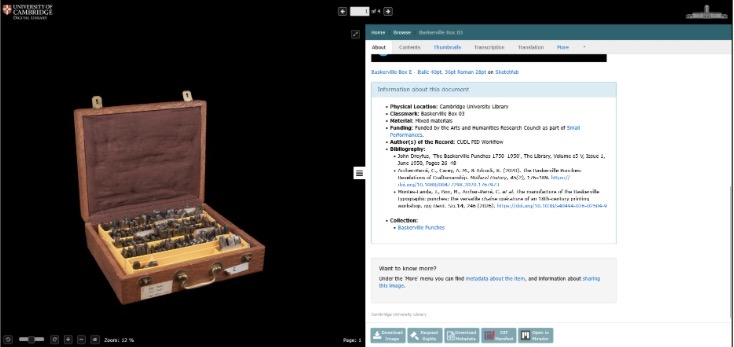
\includegraphics[width=0.8\textwidth]{./images/consultation_documents/IMG_5987.jpeg} 
	\caption{Mode de consultation proposant deux visionneuses}
	\label{fig:capture_ecran_deux_visionneuses}
\end{figure}

Une attention doit porter par la Bibliothèque Cujas face à ce choix, peu courant, car pensant s'adapter au mieux aux attentes des usagers, il ne faudrait pas que cela les rendent confus face à la présence de deux visionneuses. En effet, il semble que cela ne soit pas une habitude perpétrée par les institutions patrimoniales françaises car celle-ci propose uniquement une visionneuse \ac{IIIF}. Certains ont choisi la visionneuse Universal Viewer tandis que d'autres utilisent Mirador, répondant ainsi à des objectifs différents et des attentes propres à leurs usagers.

\subsection{L'interopérabilité des données et la pérennité des identifiants (ARK)}
Pour s'intégrer au web sémantique et aux grands réservoirs nationaux, comme le projet Orion de l'\ac{ABES}, le prototype s'appuie exclusivement sur des standards ouverts. La bibliothèque doit proposer des services permettant l'utilisation brute de données ainsi que des services d'export s'intégrant naturellement dans les chaînes de travail personnelles des chercheurs. Cette appropriation de la donnée par les chercheurs se heurte aujourd'hui à la volatilité des sessions de recherche \footannexe{\nameref{annexe_A_rapport_audit}.}.La concrétisation technique de ce "carnet de lecture" — dont nous avons justifié la nécessité méthodologique au chapitre précédent au prisme des travaux d'Elina Leblanc — pose directement la question de l'architecture de gestion des sessions dans le prototype. Afin de permettre aux chercheurs de sauvegarder leurs requêtes et leurs paniers de documents sans imposer une procédure d'inscription lourde, le prototype doit articuler deux options techniques : une persistance locale des données (via le local storage du navigateur de l'utilisateur, respectueuse de la vie privée) ou un système d'authentification fédérée (de type Shibboleth/Renater). Cette seconde piste s'avère la plus robuste pour assurer la pérennité des données de recherche d'une session à l'autre et sur différents terminaux \footcite{leblancBibliothequesNumeriquesEnrichies}. 

Afin de soutenir techniquement ces besoins d'appropriation et d'éditorialisation, l'architecture du prototype intègre des dispositifs d'interopérabilité spécifiques. Plutôt que de figer les données dans un silo de fichiers statiques, le prototype implémente des briques applicatives capables de concrétiser le concept de \enquote{citation de contenus} théorisé par Antoine Isaac, Emmanuelle Bermès et Gautier Poupeau \footcite{bermesWebSemantiqueBibliotheque2013}. En pratique, cette ambition se traduit par la mise en œuvre de modules spécifiques au sein du back-office (comme CopyIdRef ou Bibliography) et par l'exposition des métadonnées sous des formats de sérialisation ouverts (\ac{XML}, \ac{JSON-LD}). En associant à chaque document une \ac{URI} pérenne et un serveur d'images \ac{IIIF}, l'infrastructure technique ne se contente plus de diffuser : elle jette les bases d'un espace dynamique de co-construction de nouveaux savoirs, directement connectable aux outils personnels des chercheurs. Dans ce troisième âge, ce traitement intellectuel est l'un des moyens utilisés par les institutions patrimoniales transformant le document-objet en un espace d'apprentissage  et de valorisation du travail scientifique réalisés par des spécialistes.

Comme nous l'avons mis en évidence lors de l'étude comparative des outils de l'ESR, l'alternative représentée par Omeka S comporte d'importantes exigences en matière de maintenance applicative. Pour la \ac{BIU Cujas}, l'enjeu ne réside donc pas dans l'adoption passive d'un système clé en main, mais bien dans la maîtrise souveraine de ses flux de travail. En faisant le choix de développer le prototype sous Python-Django, l'institution privilégie une infrastructure sur-mesure et éco-conçue, capable de s'adapter précisément aux spécificités des sources juridiques tout en limitant la dépendance à des modules tiers dont la mise à jour n'est pas garantie à long terme.

Le choix de s'appuyer sur des formats universels et des \ac{API} vise à garantir la visibilité, la réutilisation et de la diffusion des collections à l'échelle nationale. Contrairement à l'entrepôt \ac{OAI-PMH} de CujasNum, devenu difficile à moissonner voir impossible, le prototype permet de réactiver le moissonnage en le standardisant davantage. Le système intègre dorénavant des \ac{API REST} capables de délivrer des données structurées et interopérables sous formats \ac{XML} ou \ac{JSON}, rompant avec l'image en silo \footnote{\nameref{annexe_A_rapport_audit}.}. Cette architecture modulaire offre une double opportunité : elle permet à la \ac{BIU Cujas} de moissonner d'autres portails comblant ces collections physiques ainsi que d'exposer ses propres métadonnées pour être moissonnées, augmentant drastiquement la visibilité de ses fonds.

Une des fortes attentes des chercheurs repose sur la stabilité à long terme des citations et de l'accès aux ressources numériques, pour qui la fiabilité d'un lien hypertexte est une condition importante de la scientificité de leurs travaux. À cette fin, il envisage \enquote{de désigner \ac{ARK} vers la notice bibliographique plutôt que le \ac{PDF}}. A la Bibliothèque Cujas, la méthode de création des identifiants pérennes est forgé à partir \enquote{du code-barre de l'ouvrage}, garantissant le lien permanent évitant les doublons. Cela permettrait ainsi de lier numériquement la notice bibliographique à celle du catalogue \footannexe{\nameref{annexe_A_rapport_audit}.}.

\subsection{La gestion fine des droits d'accès}
La bibliothèque numérique souhaite numériser des documents sous droit à intégrer dans sa nouvelle plateforme. Tout en restant dans un cadre strictement légal, la bibliothèque se doit de réfléchir à l'accès qu'elle permet à ses documents ne pouvant être exposés librement sans contrainte. Il est nécessaire pour l'établissement d'établir clairement une charte légale indiquant distinctement ce que l'usager a le droit de faire ou non concernant un document libre de droit et celui sous droit. La première étape consiste à assortir la notice du document à une \enquote{licence Etalab et/ou Creative Commons}. Cujas aimerait développer \enquote{un flitrage des documents sous droit ou libre de droit, grâce à la balise DcRight des notices Dublin Core} \footannexe{\nameref{annexe_A_rapport_audit}.}. 

\begin{figure}[htbp]
	\centering
	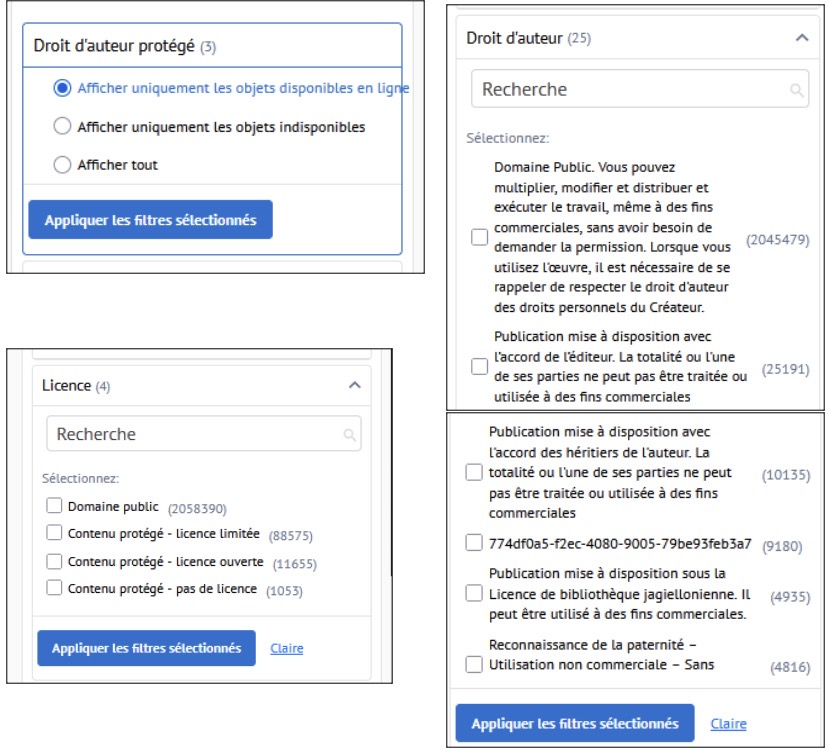
\includegraphics[width=0.5\textwidth]{./images/filtrage/IMG_5970.jpeg} 
	\caption{Différents types de filtrage dans Polona}
	\label{fig:capture_ecran_filtrage_Polona}
\end{figure}

Une des bibliothèques le fait également. Il s'agit de Polona, la bibliothèque nationale de Pologne, permettant de filtrer les documents sous droit. La deuxième étape serait de mettre en place \enquote{un horodatage débloquant le document sur le web une fois que les droits sont arrivés à terme}.

Le prototype permet de mettre en place des protocoles d'authentification centralisée \ac{SSO} et \ac{SAML}. En s'appuyant sur la fédération d'identité de Renater, grâce à ces protocoles, le système interroge à distance les serveurs des universités partenaires comme Paris I et Paris II. Cette architecture modulaire permet d'appliquer une gestion différenciée des droits d'accès \footannexe{ \nameref{annexe_A_rapport_audit}.}. Les métadonnées descriptives restent accessible publiquement sur le Web, tandis que la consultation des images est restreinte aux droits accordés par la bibliothèque en fonction du statut occupé par la personne. Un autre moyen d'accès, plus traditionnel, est de se connecter aux postes physiques connectés au réseau intranet local au sein de Cujas.

Sous \ac{XTF}, la chaîne de travail fonctionnait de façon chronophage. A l'origine, les experts métiers travaillaient de manière étanche, et toute modification de l'interface publique, une correction de coquille ou une mise en valeur éditoriale nécessitait l'intervention manuelle du service informatique. Le système était perçu comme une \enquote{boîte noire technique} par les experts métiers. Pour décloisonner ces processus, le prototype introduit un \enquote{back-office collaboratif structuré autour de profils et de rôles spécifiques}\footannexe{\nameref{annexe_A_rapport_audit} .}. 

Sur le plan de l'administration sémantique, Thomas Chaineux souligne qu'un tel environnement \enquote{répond à ses objectifs d’accès simplifié} et permet de \enquote{s’affranchir de la moindre écriture en format \ac{XML}/\ac{RDF}, \ac{JSON-LD} ou autre Turtle, grâce à l’ergonomie de son interface}. Pour la mise en valeur et l'éditorialisation, \enquote{la création de ces pages est simplifiée, de sorte qu’aucune compétence en modélisation de page Web (\ac{HTML} ou CSS) n’est requise}, l'écriture s'effectuant via une interface d'édition visuelle intuitive \footcite{chaineuxLentreeDansWeb}.

Cette autonomie s'accompagne d'une sécurisation des données grâce à la mise en œuvre de resource templates, définis par Thomas Chaineux comme \enquote{des formulaires [...] permettant de s’assurer que toutes les entités seront décrites de la même manière}, ce qui facilite la transmission et garantit la pérennité des schémas documentaires au fil du temps. Enfin, à l'image des rôles d'administration d'un \ac{CMS} sémantique, le système \enquote{propose des solutions différentes selon le statut de l’utilisateur}, permettant par exemple à un chercheur d'éditorialiser un fonds spécifique de manière autonome, tout en réservant l'accès à la base de données globale aux seuls administrateurs techniques \footcite{chaineuxLentreeDansWeb}. Cette gestion des rôles permettrait à la Bibliothèque Cujas, par exemple, \enquote{à un agent ou à un chercheur de rédiger et publier un texte sur le fonds qu'il a traité, sans pour autant lui donner les droits d'administrateur global sur tout le système}\footannexe{\nameref{annexe_A_rapport_audit}.}.    

\section[Dilemme de l'infrastructure]{Le dilemme de l'infrastructure: entre le sur-mesure et le standard}
La refonte de la bibliothèque numérique de la \ac{BIU Cujas} soulève une interrogation stratégique dépassant la simple technique informatique : quel modèle d'infrastructure privilégier pour garantir à la fois l'indépendance et l'adéquation aux besoins scientifiques et la pérennité de l'outil ? En ingénierie documentaire, c'est une question classique opposant la logique du développement spécifique, incarné par le prototype Codex, à celle de l'adoption d'outil standard, comme Omeka S.

\subsection{L'analyse du sur-mesure}
Le choix initial de la Bibliothèque Cujas, en développant le prototype Codex, offre une flexibilité totale et une forte adaptation aux besoins métiers. Cela évite également la dépendance finiancière et technique vis-à-vis d'un prestataire externe, \enquote{qui facture cher la moindre évolution}. Conçu en Python-Django, Codex offre l'avantage de s'interfacer dans la façon de travailler des experts métiers. Ce couplage permettrait  d'automatiser certaines tâches de la chaîne de numérisation de Cujas, comme la génération de métadonnées \ac{METS} ou \ac{XML}, ou des transferts sécurisés vers le serveur d'archivage du \ac{CINES}.

Si l'adaptation aux besoins est forte, ce mode de développement démontre une extrême vulnérabilité humaine, identifiée, par le directeur de la bibliothèque. Il le perçoit comme un risque de pérennité de l'infrastructure en bâtissant la future bibliothèque numérique uniquement sur les compétences d'une seule personne. En effet, Olesea Dubois confirme cette analyse : \enquote{le plus gros soucis avec les outils maisons c'est qu'ils sont très souvent associés à des personnes et à des procédures qui leur sont propres}\footannexe{\nameref{annexe_A_rapport_audit}}[pour voir l'entretien réalisé auprès d'Olesea Dubois]. Un autre inconvénient mis en avant par la responsable de la bibliothèque numérique de Sciences Po est que \enquote{généralement, il y a peu ou pas assez de documentations entraînant ainsi une durée de vie assez courte de la bibliothèque numérique} \footannexe{\nameref{annexe_A_rapport_audit} pour voir l'entretien avec Olesea Dubois.}. Effectivement, le peu de documentation disponible entraîne un risque pour la pérennité de l'outil, et empêche le maintien sur le long terme de la bibliothèque numérique. Avoir recours à un logiciel sur-mesure entraîne une difficulté de recrutement, car l'institution se coupe d'un vivier de compétence, rendant rapidement le code sur-mesure inexploitable en cas du départ de son concepteur, condamnant le système à une obsolescence rapide. La crainte de la plupart des institutions patrimoniales y compris la bibliothèque Cujas est de reproduire la situation qui a entraîné la disparition de la bibliothèque numérique Medica. C'est pour pallier à cela qu'elles ont choisi de se tourner vers des outils standardisés afin de disposer d'un vivier de personnel.

La tension entre le développement d’un prototype sur-mesure et l’adoption d’un standard communautaire comme Omeka S s'inscrit au cœur des réflexions sur la souveraineté technique et la maîtrise de l'obsolescence logicielle au sein des institutions patrimoniales\footcite{bermesWebSemantiqueBibliotheque2013}. D'un côté, le développement interne d’une solution ad hoc, à l'instar du prototype \textit{Codex} conçu sous Python-Django, s'impose comme une réponse souveraine et immédiate face à l'urgence fonctionnelle : il permet de pallier la fragilité de CujasNum sous l'infrastructure obsolète \ac{XTF} et d'assurer une continuité absolue du service public de la recherche face aux risques de sécurité informatique. 

Toutefois, cette autonomie technique se heurte rapidement aux limites de la maintenance à long terme d'un outil isolé. À l'ère de la Transition bibliographique, la rapidité des évolutions technologiques rend en effet indispensable l'adossement à une communauté active pour éviter qu'une institution ne se retrouve marginalisée par des services rapidement dépassés. C'est ici que l'adoption d'un standard libre et communautaire tel qu'Omeka S révèle sa force stratégique. En s'appuyant sur un code source ouvert, l'établissement lutte activement contre l'obsolescence logicielle souvent entretenue par les éditeurs de logiciels propriétaires\footcite{creusotQuellesPerspectivesPour}. De plus, en permettant un déploiement et un hébergement locaux — contrairement aux offres propriétaires en mode SaaS (\textit{Software as a Service}) sur le cloud —, un outil comme Omeka S garantit à l’institution la maîtrise absolue de ses données et de ses choix d'archivage, réalisant un compromis idéal entre les impératifs du modèle sémantique sémantisé (RDF, Dublin Core) et l'utilisabilité de l'interface\footcite{chaineuxLentreeDansWeb, creusotQuellesPerspectivesPour}.


\subsection{L'analyse du standard communautaire}
Face au risque d'isolement technique du sur-mesure, les retours d'expérience des responsables de bibliothèque numérique des institutions patrimoniales comme la Bibliothèque Sainte-Geneviève, la Bibliothèque de Sciences Po ou l'\ac{ENS}, démontrent un abandon progressif des outils sur-mesure au profit d'Omeka S. Financé par des subventions de recherche, de fondations et soutenu par une communauté, Omeka S offre des garanties majeures de durabilité. Comme le résume Thomas Chaineux, ce logiciel représente \enquote{un compromis entre les impératifs du modèle et l'ergonomie}, s'imposant pour les \ac{BU} moyennes comme \enquote{une porte d'entrée bienvenue} grâce à sa gratuité et la force de son réseau communautaire \footcite{chaineuxLentreeDansWeb}. Contrairement à Django qui nécessite d'avoir des compétences informatiques avancées pour développer le logiciel et l'intégrer dans le web sémantique. La particularité d'Omeka S est d'avoir été pensé pour s'intégrer directerement ou plus facilement dans le web de données. Il s'appuie sur une \enquote{modélisation des métadonnées sous \ac{RDF}} combinées à des vocabulaires standardisés, comme le Dublin Core, qui favorise \enquote{une meilleure exposition des données}. Il facilite l'exposition des métadonnées, leur exportation et leur interopérabilité. 
 
De plus, un autre des avantages pour les catalogueurs est de \enquote{bénéficier d'un back-office documenté, collaboratif et modulaire}. Toutefois, malgré les avantages certains, l'environnement Omeka S s'accompagne de contraintes réelles. Bien qu'open-source, le logiciel est \enquote{gratuit}, mais il exige des ressources pour fonctionner et évoluer. Omeka S demande des ressources internes pour en assurer l'hébergement, le paramétrage et la maintenance technique. Gilles Clément, l'un des concepteurs de NuBIS, témoigne de cette limite : \enquote{À l'usage, chaque nouvelle version d'Omeka S cassait quelque chose[...]. Nous étions confrontés à beaucoup de bidouillages en raison de l'instabilité des modules tiers développés par des prestataires différents, ce qui rendait le code lourd et difficile à maintenir} \footannexe{\nameref{annexe_A_rapport_audit} pour voir l'entretien avec Cécile Obligi et Gilles Clément de la \ac{BIS}.}. Cette instabilité fait écho à l'analyse de Thomas Chaineux, qui situe Omeka S dans \enquote{une position hybride dans le Web de données}. Faute d'émettre des \ac{URI} nativement pérennes à l'échelle globale sans développements tiers, le logiciel génère par défaut des \enquote{noeuds blancs} dont la portée reste limitée au contexte local \footcite{chaineuxLentreeDansWeb}. 
 
Face à cet obstacle, la solution mise en place par la \ac{BIS} pour le résoudre, a été de séparer techniquement le front du back, \enquote{rendant ainsi le code-source plus maintenable dans le temps} \footannexe{\nameref{annexe_A_rapport_audit} pour voir l'entretien avec Cécile Obligi et Gilles Clément de la \ac{BIS}.}. En effet, à chaque mise à jour, le module complémentaire déréglait les paramétrages du front-office. La \ac{BIS} a donc découplé son architecture en décidant de \enquote{développer leur back-office sous Omeka S et du front sous Astro.js} \footannexe{\nameref{annexe_A_rapport_audit} pour voir l'entretien avec Cécile Obligi et Gilles Clément de la \ac{BIS}.}. Cette distinction rend étanche les couches logicielles permettant ainsi le bon fonctionnement de NuBIS et la satisfaction des équipes qui en sont en charge. Malgré cet obstacle rencontré par certaines institutions, l'open-source, contrairement au sur-mesure, a cette \enquote{notion de mutualisation rendant plus facile l'idée du maintien de cette structure} \footannexe{\nameref{annexe_A_rapport_audit} pour voir l'entretien avec Vincent Tardif de l'\ac{ENS}.}. Le choix de la \ac{BIS} du framework Astro.js répond à des exigences d'éco-conception et d'accessibilité numérique, évitant ainsi l'interrogation de la base à chaque clic de l'usager. L'avantage majeur de ce type de fonctionnement est que les montées de versions d'Omeka S n'impactent plus l'affichage public, sécurisant mieux le back-office le rendant plus maintenable dans le temps et pérenne.
\section{Pérennité, maintenance et gestion des risques}
Le passage d'\ac{XTF} vers un nouveau système ne se limite pas uniquement à un arbitrage d'ingénierie logicielle. Il constitue un défi de gouvernance et de gestion des ressources humaines et de viabilité du logiciel sur le long terme pour la Bibliothèque Cujas.

Tout d'abord, à l'instar d'autres bibliothèques, l'ensemble de l'infrastructure technique repose principalement sur les compétences d'une seule personne. Ce constat d'une dépendance extrême est reconnu par le directeur et les experts métiers, attendant avec la nouvelle infrastructure d'avoir une meilleure visibilité dans le back-office. Pour éviter de créer à nouveau une \enquote{boîte noire} et d'abrégrer prématurément la durée de vie de la bibliothèque numérique, toute refonte doit alors s'accompagner d'une documentation fonctionnelle et technique très détaillée \footannexe{\nameref{annexe_A_rapport_audit}.}. Cette documentation permet ainsi de comprendre et de justifier les choix qui ont été fait. Elle doit consigner \enquote{chaque choix de circuit, l'architecture des bases de données, le code des \ac{API} et la configuration des serveurs} permettant ainsi de disposer d'une compréhension globale dans le cas du départ du concepteur, remplacé par une autre personne assurant sa pérennité \footannexe{ \nameref{annexe_A_rapport_audit}.}.
	
	\begin{figure}[htbp]
		\centering
		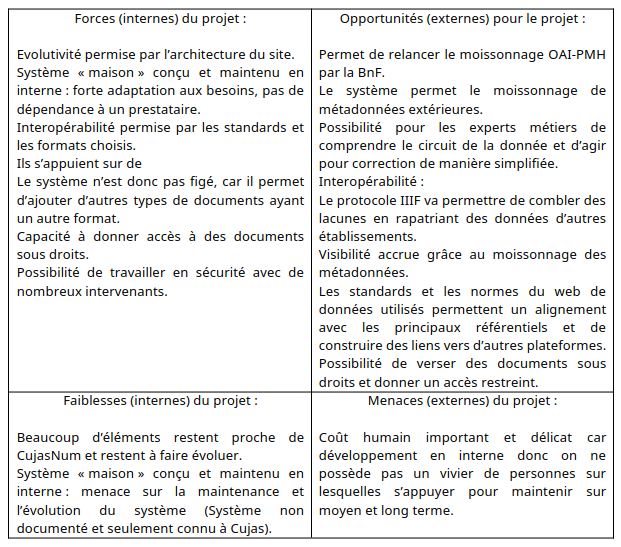
\includegraphics[width=0.5\textwidth]{./images/Screenshot from 2026-09-07 20-54-20.png} 
		\caption{Réalisation d'un SWOT pour le prototype}
		\label{fig:capture_ecran_SWOT}
	\end{figure}
	
	
Le choix de pérenniser un prototype sur-mesure amène la Bibliothèque Cujas à devoir assurer la totalité de \enquote{l'effort de maintenance corrective en interne, de mise à jour des sécurités et à l'adaptation à de futurs standards} \footannexe{\nameref{annexe_A_rapport_audit}.}. Or, la Bibliothèque Cujas ne dispose pas d'un vivier de développeurs permettant d'assurer un suivi de la bibliothèque numérique. À l'inverse de la maintenance d'un système open-source qui permet de partager l'effort, réduisant la charge technique.

La refonte de la bibliothèque numérique de la Bibliothèque cujas ne saurait se résumer uniquement à un simple chantier informatique. Les choix d'infrastructure posent les fondations matérielles et logicielles indispensables à la pérennité, à la sécurité et à l'interopérabilité des collections patrimoniales. Cependant, aussi évolué que peut être l'ingénierie logicielle, elle ne serait être validée si elle ne s'adapte pas aux pratiques contemporaines de la recherche. Il est donc nécessaire d'évaluer comment mettre en place des services fluides adaptés à l'usage.
\chapter[L'usage au centre du changement]{L'usager au centre de ce changement : la traduction des besoins en services fonctionnels et ergonomiques}

\lettrine{L}a valeur scientifique d'une bibliothèque numérique se mesure aussi à la conception des services mis en place par la bibliothèque pour répondre aux besoins identifiés de ses usagers. Le passage au prototype représente un changement majeur pour la Bibliothèque Cujas, permettant de mettre ne place une éditorialisation, adaptée aux différents types de public du lecteur éclairé au chercheur chevronné.
Dès lors, les retours d'expérience des chercheurs interrogés révèlent l'attente fondamentale: celle de retrouver un confort d'étude et la maniabilité aussi proches que celle d'un livre physique. Le défi de la refonte de la bibliothèque numérique consiste à concilier deux attentes : la \enquote{trouvabilité} et la \enquote{découvrabilité}, s'adaptant ainsi aux pratiques contemporaines de la recherche.

\section{L'interface de recherche et d'affichage}
Historiquement, CujasNum révèle que si le moteur de recherche simple s'avérait robuste et tolérant aux troncatures, l'interface souffrait quant à elle de visibilité et d'une confusion entre les différents modes de recherche. Le prototype a jeté les bases de la modernisation, mais révèle des limites ergonomiques en multipliant et en répétant les onglets de recherche à différents endroits, créant une surchage cognitive. Pour surmonter ces inconvénients et répondre aux attentes des chercheurs, l'interface doit s'articuler autour de trois modalités : la recherche épurée, des filtres restructurées et des options de tri.

\subsection{La recherche simple par barre unique}
Sur CujasNum, les usagers étaient régulièrement confrontés à un bruit documentaire, ou à l'inverse à des silences inexplicables causé par la confusion entre la recherche dans les notices et la recherche plein-texte. Pour y remédier, la future page d'accueil de la bibliothèque numérique proposera une barre de recherche simple unique, positionnée au centre de l'interface. L'usager doit pouvoir sélectionner explicitement son périmètre via trois options de recherche simple : \enquote{à travers les métadonnées, la recherche s'effectue dans les notices descriptives ; à travers le plein-texte, la recherche interroge les textes océrisés et la dernière option est la combinaison des métadonnées et du plein-texte, la recherche s'effectue alors en croisant les données textuelles et descriptives de la plateforme} \footannexe{\nameref{annexe_B_preconisations}.}.

Ce modèle de recherche s'inspire des pratiques de recherche et d'autres institutions patrimoniales, comme la \ac{BIS} ou l'\ac{INHA}, qui ont été développées au sein de leur propre bibliothèque numérique. Cette répartition permet d'accompagner le lecteur éliminant ainsi toute ambiguïté. Cette barre simple disposera d'un système d'autocomplétion ou de saisie intuitive, guidant l'usager dans sa recherche.

\subsection{La recherche avancée multicritères}
Dans CujasNum, le formulaire de recherche avancée était synonyme de confusion pour les agents et pour les usagers, car elle se situait \enquote{sur la même page que la recherche en texte intégrale} et utilisait un vocabulaire très professionnel, comme l'intitulé \enquote{notice bibliographique} peu compréhensible pour des étudiants ou des chercheurs non-spécialistes du livre \footannexe{\nameref{annexe_A_rapport_audit}.}.

La prototype proposera un bouton de recherche avancée unique, clairement visible et situé en-dessous de la barre de recherche simple. C'est une pratique de présentation devenue courante que l'on retrouve dans différentes bibliothèques numériques, comme chez Lucienne de l'\ac{ENS} ou encore Cariatide de l'\ac{INHA}. Ce mode de présentation épuré mais visible réduit la charge cognitive des usagers, reproduisant des habitudes de recherche des grands moteurs de recherche, comme Google ou Firefox \footannexe{\nameref{annexe_B_preconisations}.}. En cliquant sur le bouton de recherche avancée, l'utilisateur se trouve redirigé vers le formulaire qu'il n'a plus qu'à remplir. Ce formulaire permet ainsi de préciser des zones de recherche acceptant différents champs de saisie combiné à des opérateurs booléens.

Cette structuration permet aux chercheurs de réaliser des requêtes complexes en croisant les sources disponibles dans la bibliothèque numérique. Ce formulaire permet de répondre à l'une des attentes des chercheurs qui apprécient \enquote{de mener leur recherche à partir d'un point précis et élargissant progressivement leur périmètre de recherche au fur et à mesure} \footannexe{\nameref{annexe_A_rapport_audit}.}.

\subsection{Le filtrage par facettes}
L'un des chantiers identifiés au cours de l'audit de CujasNum se révèle être la gestion des filtres et des facettes. L'indexation historique reposait sur l'indexation propre à la bibliothèque Cujas. Cette indexatioin a généré des facettes ultra-spécifiques, souvent reliées à un seul document, comme la facette \enquote{Droit romain - Loi des Douze Tables}. Ce niveau de granularité entraînait une importante frustration pour les usagers signalant \enquote{qu'à cause de ça il n'utilisait ces facettes} ne souhaitant pas passer à côté d'un document. De surcroît, des variations de casse ou de typologies créaient davantage de facettes \footannexe{\nameref{annexe_A_rapport_audit}.}.

Une restructuration intégrale de ce parcours est envisagée par la Bibliothèque Cujas. Le filtrage sera regroupé dans une nouvelle rubrique intitulée \enquote{Explorer}. La bibliothèque numérique proposera un ensemble de facettes générales et normalisées applicables à plusieurs types de documents \footnote{\nameref{annexe_A_rapport_audit}.}. Cette restructuration permettra ainsi aux usagers de mieux comprendre comment sont présentée les collections. En effet, comme le démontre Leblanc \enquote{les facettes reflètent la manière dont la bibliothèque numérique a pensé ses collections et aident ainsi l'utilisateur à apprendre empiriquement l'organisation des collections} \footcite{leblancBibliothequesNumeriquesEnrichies}. Ce système de facettes permet ainsi la Bibliothèque Cujas de guider intellectuellement les usagers. Un bon système de guidage bien formé et pensé devient un service indispensable \enquote{et permettent d'éviter le phénomène de surabondance des choix}.

Le système de filtrage ou de tri est tout aussi important que les autres modes de recherche, et nécessite d'être bien pensé. La simplification de l'indexation et des différents modes de recherche évite la confusion de l'usager, complétant ainsi les autres services proposés par la bibliothèque numérique. 
\section{L'Espace personnel et les services des chercheurs}
La refonte de la bibliothèque numérique de Cujas doit s'affranchir d'une consultation passive de l'interface en un véritable espace de travail personnalisé tout en y adossant des outils d'analyse scientifique avancées.

\subsection{L'intégration du standard IIIF et de la visionneuse Mirador}
Sur CujasNum, à l'origine, la consultation des ouvrages reposait sur une visionneuse \ac{JPEG}, de bonne qualité. De plus, elle offrait également la possibilité de télécharger le document consulté sans format \ac{PDF} sans offrir différentes options de téléchargements ou d'autres formats. Un des chercheurs expliquait qu'il était peu courant qu'une bibliothèque offre différentes options de téléchargement, qu'il trouvait cela dommage car par moment il aurait bien aimé pouvoir choisir uniquement de télécharger les pages intéressantes pour son étude. Une doctorante mentionne le fait que ce serait bien d'ajouter en plus des options de téléchargement \enquote{la possibilité de conserver la page de titre de l'ouvrage} \footannexe{\nameref{annexe_A_rapport_audit}.}. De cette façon, l'usager peut retrouver la source du document.

Pour répondre à ces attentes, le prototype Codex, développé par la Bibliothèque Cujas, sépare la couche de diffusion de celle de conservation, grâce à l'implémentation d'un serveur \ac{IIIF}. Ce standard permet la diffusion dynamique d'image accompagnée d'outils scientifiques, proposant la possibilité de réaliser des captures d'écran, des annotations.

L'implémentation de la visionneuse Mirador offre l'opportunité aux chercheurs de la comparaison des documents au sein d'un même espace de travail. Les chercheurs peuvent désormais consulter plusieurs ouvrages afin de mener des analyses comparatives. Un autre des avantages est la possibilité d'utiliser un zoom profond sur une image exposée en haute définition. Elle offre aussi des réglages de rotations d'images, de contrastes et de colorimétrie.

\subsection{L'espace personnel du chercheur}
Cette transition vers des espaces personnels et des outils d'extraction personnalisés répond à l'acculturation croissante des chercheurs aux humanités numériques, exigeant désormais de manipuler directement la donnée sémantique plutôt que de simples fichiers statiques\footcite{mesguichBibliothequesFaceMonde}

L'enquête de terrain et les entretiens menés auprès des usagers révèlent leur souhait d'avoir leurs propres espaces de  travail pour mener à bien leurs recherches. Sous CujasNum, ils avaient pris l'habitude de télécharger chaque document ne pouvant les conserver une fois le navigateur fermé.

Pour ancrer durablement l'usager dans la bibliothèque numérique de Cujas, l'implémentation d'un espace personnel est une priorité fonctionnelle majeure. Cet espace proposera des services simples et intuitifs comme la gestion des favoris, l'archivage des requêtes, et la recherche ciblée dans les sélections. L'espace personnel offre aussi la possibilité de rédiger des notes de travail ainsi que des annotations personnelles. Comme l'a expliqué Elina Leblanc, l'espace personnel répond à un besoin d'archivage d'usage. Il s'agit comme \enquote{une barrière à l'oubli} et génère \enquote{une économie de temps} cruciale pour les chercheurs \footcite{leblancBibliothequesNumeriquesEnrichies}.

\subsection{L'exposition des données}
Afin d'accompagner les usagers dans leurs rédactions, le prototype Codex doit offrir la possibilité des services d'exportation des données et d'analyse linguistiques aux standards du web sémantique.

Les chercheurs interrogés s'accordent sur l'importance d'intégrer des fonctionnalités d'export des références bibliographiques normalisées afin de fluidifier la constitution de leurs propres corpus de travail. Cette attente pragmatique fait directement écho aux constats d'Antoine Courtin, évoqués précédemment, concernant les pratiques réelles des chercheurs, dont les usages numériques s'ancrent d'abord dans des gestes simples de récupération et de manipulation directe de données textuelles. Afin de concrétiser cette attente au sein de l'interface, le prototype Codex mobilise le module open-source Bibliography d'Omeka S. Cette intégration rend possible l'exportation instantanée de la notice bibliographique vers des gestionnaires de références d'usage courant, comme Zotero ou EndNote, sous des formats interopérables standardisés (tels que BibTex, RIS ou JSON-LD) \footannexe{\nameref{annexe_A_rapport_audit}.}.

L'intégration du format \ac{XML-TEI} s'impose comme le standard pour encader la structure logique des textes juridiques, facilitant ainsi la reconnaissance des entités nommées (personnalités citées, lieux, date) et permet la fouille de texte. Comme l'expliquent Emmanuelle Bermès et Gautier Poupeau, la fouille de texte est rendue possible grâce à la disponibilité des corpus. \enquote{La \enquote{fouille de textes et de données}(en anglais \textit{text and data mining} ou \ac{TDM}) embrasse un nouveau paradigme dans l'accès aux documents ou aux sources, qu'on pourrait désigner sous le nom de lecture distante, dans la lignée de Franco Moretti} \footcite{bermesTroisAgesNumerique}.L'intérêt fondamental du \ac{TDM} permet d'exploiter la masse de textes désormais numérique s'affranchissant des limites physiques de la lecture traditionnelle.

En dotant l'usager d'outil de pointe comme une visionneuse Mirador, un compte personnel et des formats structurés, la bibliothèque numérique devient un véritable outil pour mener à bien les projets en humanités numériques. Afin de mettre en avant cette collaboration entre les chercheurs et la bibliothèque, l'infrastructure doit alors s'accompagner d'une médiation intellectuelle. 
\section{Valorisation scientifique des collections}
L'éditorialisation constitue désormais un maillon indispensable pour donner de la cohérence intellectuelle à une bibliothèque numérique. L'éditorialisation contextualise les fonds, guide l'usager et valorise l'expertise scientifique de l'établissement.

Lors des enquêtes de terrains, les chercheurs ont fortement insisté sur la mise en place de cette médiation. L'un des chercheurs souligne qu'actuellement dans CujasNum, cela manque parfois de textes explicatifs, notamment sur la constitution des collections ou explicitant les choix de classifications. De même, un autre professeur rappelle l'importance d'attirer l'attention des usagers sur le contenu et la valeur singulière des ouvrages anciens.

Pour mettre en place cette médiation culturelle sans alourdir l'infrastructure technique, la bibliothèque Cujas peut s'inspirer du fonctionnement de la BIS. Lors de la conception d'expositions virtuelles ou de billets d'actualité, la \ac{BIS} renonce à l'utilisation d'exposition virtuelles intégrées dans des visionneuses lourdes et peu portables. Elle a donc décidé d'opter pour le format Markdown. Les billets de blog et les pages d'expositions deviennent de simples fichiers textes structurés par des balises Markdown très légères, et exportables d'une solution technique à une autre. Ce choix technique permet de s'affranchir des instabilités des extensions de \ac{CMS}, assurant une pérennité des données.

Pour rationaliser et homogénéiser la production éditoriale scientifique écrite par des tiers, la plateforme doit appliquer une démarche de qualité rigoureuse inspirée du guide de NuBIS \footcite{sorbonneBlog2026}. Ce guide impose des règles strictes autour de trois points : la gestion des images, les contraintes rédactionnelles et le respect des droits d'auteur. Le respect de ces trois règles imposent un cadre strict que doivent suivre les chercheurs souhaitant participer à l'éditorialisation de leur bibliothèque numérique \footcite{sorbonneExpositionsVirtuelles}. Comme l'a expliqué Elina Leblanc qui a analysé les \enquote{expositions nativement numériques} comme des espaces collaboratifs de recherche. Elle parle des avantages de permettre à des chercheurs, des enseignants ou des doctorants de rédiger des focus ou des notices scientifiques \enquote{participe au processus d'éditorialisation et conduit ainsi à créer de nouveaux savoirs, pouvant à leur tout être partagés} \footcite{leblancBibliothequesNumeriquesEnrichies}.

\subsection{Les formats de valorisation}
En s'appuyant sur ces règles de rédaction, l'éditorialisation scientifique de la \ac{BIU Cujas} se déploiera sous plusieurs formes complémentaires, pensés pour différents niveaux de lecture, comme la Galerie des grands juristes et l'éditorialisation par des juristes pour des juristes.

La \enquote{Galerie des grands juristes} est proposé par le directeur de la Bibliothèque Cujas. Cette entrée thématique prendra la forme d'une galerie de portraits intéractifs, inspirée de la même idée que la Bibliothèque de l'\ac{ENS} qui a mis en avant ces collections, sous le nom des \textit{Parcours normalien.ne.s} \footannexe{\nameref{annexe_B_preconisations}.}. Chaque juriste fera l'objet d'une notice biographique, compris entre 5 000 et 10 000 signes, rédigée par un chercheur. Depuis la fiche bibliographique de l'auteur, l'usager pourra rebondir instantanément sur l'ensemble de ses oeuvres numérisées disponible dans la Bibliothèque Cujas ou sur des sites partenaires.

Une deuxième forme d'éditorialisation des collections sera d'écrire des billets de blog, des parcours thématiques, faits par des spécialistes sur une question ou une thématique. Cela pourrait également, comme le suggérait l'un des enseignant-chercheur, créer une porte d'entrée aux jeunes chercheurs dans développement de leur carrière. L'ancienne responsable de la bibliothèque numérique rappelle l'intérêt d'associer directement les étudiants avancés et les chercheurs à cette démarche de valorisation. L'idée serait de permettre à des chercheurs ou des étudiants d'écrire des articles des billets de blog sur un ou des documents étudiés provenant de la Bibliothèque Cujas, et là le replacer dans un contexte intellectuel, redonnant \enquote{vie} aux documents numérisés \footannexe{\nameref{annexe_B_preconisations}.}. Laurent Pfister pense que ce serait un excellent moyen de valoriser la production scientifique notamment pour des jeunes chercheurs.

En combinant la flexibilité technique du format Markdown et la rigueur des guides d'expositions de la \ac{BIS}, la bibliothèque numérique de Cujas ne sera plus uniquement un outil d'exposition de ses documents numérisés, mais deviendra une véritable plateforme de médiation culturelle juridique. Pour que ces services soient utilisés par les usagers, il est nécessaire pour les experts métiers de les accompagner dans leur prise en main. Il est important alors que les experts métiers eux-mêmes soient capables de les utiliser amenant le service dédié de la bibliothèque à les accompagner dans la conduite du changement.
\chapter[Les défis de gouvernance de cette refonte]{Les défis de gouvernance de cette refonte : conduite du changement et décloisonnement}

\lettrine{L}'implémentation d'une architecture logicielle moderne et la conception de services numériques orientés usagers ne sauraient à elles seules garantir le succès d'une refonte si elle ne s'accompagne pas d'une restructuration interne de l'établissement. En effet, la réussite d'un projet de bibliothèque numérique repose sur plusieurs facteurs fondamentaux : humains, financiers et organisationnels.

Dès lors, le premier enjeu de gouvernance réside dans le décloisonnement de ces circuits. L'introduction d'un back-office collaboratif structuré autour de rôles métiers précis vise à redonner une véritable autonomie opérationnelle à l'équipe de conservation. Cependant, comme le souligne le projet Orion, le passage d'une simple production artisanale à une gestion de données modernisée ne se décrète pas par un simple choix de changement de logiciel. Il exige d'accompagner étroitement les agents, dans ce projet, pour les aider à abandonner d'anciennes habitudes de travail et à inventer collectivement de nouveaux circuits documentaires. 

Cette conduite de changement est nécessaire pour intégrer de nouveaux services. Parallèlement à ce travail, une veille documentaire fonctionnelle et technique s'impose afin d'assurer la pérennité de la future bibliothèque numérique de Cujas.
\section{L'évolution des métiers et des pratiques}
La réussite technique et ergonomique de la refonte de la bibliothèque numérique ne peut se concevoir indépendamment d'une restructuration des circuits de travail humains de l'établissement. L'analyse historique et organisationnelle de la \ac{BIU Cujas} révèle que la rigidité des outils informatiques passés a non seulement figé l'interface publique, mais a également façonné, voire contraint, l'organisation des équipes internes, créant des cloisonnements.

\subsection{L'état des lieux: un double cloisonnement}
L'analyse de l'organisation interne de la \ac{BIU Cujas} révèle que les difficultés ergonomiques et éditoriales de CujasNum sont le résultat d'un double cloisonnement humain et logiciel.

Sur le plan organisationnel, la bibliothèque a été marquée par une restructuration de ses services dans le courant de l'année 2018, entraînant une importante rupture structurelle. L'un des exemples est le service informatique qui s'est scindé en deux services distincts : d'un côté, le Département d'informatique technique \ac{DIT} et de l'autre, le Département d'information documentaire \ac{DID}) \footannexe{\nameref{annexe_A_rapport_audit} pour voir l'entretien du \ac{DID}.}. Cette séparation nette entraîne un cloisonnement dans la réalisation des tâches. La spécialisation de compétence était nécessaire, mais a pour effet indirect d'éloigner les experts métiers de la gouvernance technique de la bibliothèque numérique.

Ce cloisonnement humain s'est retrouvé renforcé par l'architecture logicielle de la bibliothèque CujasNum. Le traitement documentaire et la mise en ligne fonctionnaient auparavant de façon totalement distincte : le service du patrimoine traitait des métadonnées dans le catalogue de la bibliothèque sans aucune visibilité sur le rendu final, tandis que l'implémentation des fichiers sur le serveur public s'opérait de manière automatique par des scripts en arrière-plan \footannexe{\nameref{annexe_A_rapport_audit} pour voir l'entretien avec Mebrouk Leulmi.}.

Cette opacité a transformé le back-office de CujasNum en une véritable \enquote{boîte noire} technique pour les équipes du \ac{DID} et du \ac{DPCN}. La moindre correction, dans CujasNum, demandait la sollicitation permanente du responsable du \ac{DIT} \footannexe{\nameref{annexe_A_rapport_audit} pour voir l'entretien avec Grégory Colcanap.}. Cette dépendance a ralenti le rythme de mise en valeur scientifique des fonds, mais elle a également démobilisé les agents du métier, privés de toute autonomie et de visibilité sur l'impact de leur travail dans la chaîne de production.

\subsection{Redonner l'autonomie aux métiers grâce à Codex}
Pour rompre cette dépendance technique et fluidifier les processus internes, la conception du prototype Codex introduit un changement considérable, en se basant sur un back-office collaboratif et administrable par le métier au centre de son architecture. C'était d'ailleurs l'une des attentes du \ac{DID} à propos de la refonte que \enquote{le back-office soit administrable par un bibliothécaire} \footannexe{\nameref{annexe_A_rapport_audit} pour voir l'entretien du \ac{DID}.}.

Développé en Python-Django, le prototype Codex permet la mise en place d'une gestion fine des rôles à attribuer autour des rôles métiers spécifiques et des tâches qu'ils ont à effectuer. Par exemple, \enquote{le catalogueur administre et enrichit les métadonnées descriptives en lien direct avec le \ac{SUDOC} et Alma. L'éditeur de contenu rédige les actualités, éditorialise les pages d'accueil des collections et crée des parcours thématiques} \footannexe{\nameref{annexe_A_rapport_audit} pour voir l'entretien avec Mebrouk Leulmi.}. Le technicien en contrôle qualité valide la qualité des images numérisées par les prestataires extérieurs avant leur versement et s'assure de l'avancement des différents lots.

Grâce à cette répartition des droits d'accès au sein de la partie administrative du prototype Codex, le \ac{DPCN} et le \ac{DID} auront une meilleure visibilité des différentes étapes de production à l'intérieur. Ils pourront également réaliser les micro-corrections sans dépendre constamment du responsable du \ac{DIT}, permettant une meilleure répartition du travail. Le \ac{DIT} peut s'occuper alors de la maintenance technique de la plateforme \footannexe{\nameref{annexe_A_rapport_audit} pour voir l'entretien avec Mebrouk Leulmi.}.

\subsection{La conduite du changement}
Comme le rappelle Catherine Storne-Sengel, la réussite d'un projet de réinformatisation ou de refonte documentaire ne dépend pas seulement de la performance de la nouvelle infrastructure, mais repose fondamentalement sur l'accompagnement des agents face aux mutations de leurs pratiques quotidiennes\footcite{storne-sengelAccompagnerChangementsPratique2017}.

Le passage d'un mode de production caractérisé comme artisanal à une plateforme ouverte et collaborative exige d'accompagner étroitement les équipes face à ce changement. En effet, comme le souligne le rapport du projet Orion, l'accompagnement des agents est nécessaire pour mettre en place de nouvelles pratiques de travail ou celles existantes.

Cette conduite du changement doit s'opérer autour de trois axes : former aux nouveaux standards du web sémantique, clarifier les responsabilités dans le workflow, et valorisation du contenu scientifique. En effet, les gestionnaires de données et les catalogueurs doivent être formés aux nouveaux standards du web sémantique, afin d'être capable de réutiliser des alignements sur des référentiels nationaux, comme IdRef \footcite{martinolliEnrichirSesDonnees2025}, de sorte que les notices des documents numérisés créées permettent de s'interconnecter à d'autres grâce à ce référentiel. De plus, il est important de clarifier les droits des différentes personnes dans le workflow afin que les automatisations ne les bloquent pas dans leur travail. Il faut également qu'ils puissent comprendre comment leur travail impacte le reste de la production. Le rôle du bibliothécaire évolue pour devenir un \enquote{Digital Librarian}. Comme l'a théorisé Sneerivasulu, dans les années 2000, le passage du bibliothécaire traditionnel au bibliothécaire numérique, véritable \enquote{ingénieur des connaissances chargé de créer et d'organiser des canaux de diffusion sémantiques interconnectés}.

Les bibliothécaires auront dans Codex différents espaces de valorisation pour les collections ou les actualités de la bibliothèque numérique. Ils peuvent être amené à rédiger des tutoriels afin de permettre aux chercheurs de prendre en main les nouveaux outils à leur disposition.
\section[Médiation et autonomie]{La médiation numérique et l'autonomie des chercheurs}
Le passage d'un outil figé à une plateforme dynamique ne relève pas uniquement d'un alignement technique, il s'inscrit aussi dans une mutation des pratiques professionnelles. À la Bibliothèque Cujas, cette conduite du changement doit permettre d'alléger la charge de travail et valoriser l'expertise métier des agents.

\subsection{La médiation et l'autonomie des chercheurs}
La mise en place d'un back-office collaboratif redistribue les rôles et modifie le quotidien des agents. L'analyse fonctionnelle réalisée dans le cadre de la réalisation de l'audit permet d'identifier l'évolution du rôle d'accompagnent des personnels des bibliothèques. 

Les bibliothécaires, étant au contact du public, ont besoin de connaître avec précision les services de la bibliothèque et d'être en mesure d'expliquer son fonctionnement. Ils doivent aussi pouvoir répondre aux questions éventuelles que les usagers pourraient être amenés à leur poser. Leur motivation première est d'accompagner les usagers pour les rendre autonome dans leur appropriation des outils. Face à l'arrivée de briques technologiques complexes, comme la visionneuse Mirador ou le serveur \ac{IIIF}, la conduite du changement place le bibliothécaire dans un rôle de médiateur permettant de rendre autonome le chercheur. Dans cette nouvelle posture, il est amené à rédiger des tutoriels ou des pages d'aide pour les différents publics de la bibliothèque \footannexe{\nameref{annexe_B_preconisations}.}.

Le responsable de la bibliothèque numérique se doit d'avoir une bonne compréhension globale de son infrastructure. C'est sur cette connaissance qu'il pourrait s'appuyer dans le cadre de la réalisation de projet scientifique en collaboration avec les chercheurs afin de pouvoir mettre en avant les collections numérisées.La future bibliothèque numérique doit devenir un espace collaboratif favorisant l'appropriation active et autonome des sources présentes à l'intérieur \footannexe{\nameref{annexe_B_preconisations}.}.

\subsection{La co-conception des programmes documentaires}
L'histoire de CujasNum est marquée par la collaboration scientifique, notamment pour la liste Pfister-Roumy. Pour que la future plateforme demeure une référence, la bibliothèque peut envisager d'ouvrir la conception de la politique documentaire à un comité scientifique de chercheurs. Ce comité aura pour mission de définir et de prioriser de manière collaborative les futurs chantiers de numérisation. Par exemple, un des enseignants-chercheurs proposait d'initier en ce sens un nouveau projet de numérisation, nommé la \enquote{liste Pfister-Roumy 2.0} ciblant \enquote{les manuels de droits civils et les grands revues de la période de 1800 à 1940} \footannexe{\nameref{annexe_A_rapport_audit}.}. Cette collaboration permettra à la Bibliothèque Cujas de constituer des projets scientifiques cohérents et pertinents pour les chercheurs. De cette façon, le chercheur prend là une part active à la conception de la future bibliothèque numérique.

\subsection{L'éditorialisation participative}
L'un des avantages de cette refonte est l'intégration des chercheurs et des étudiants avancés au sein du processus d'éditorialisation et de valorisation des collections. CujasNum laissait peu de place à l'éditorialisation, car le logiciel ne le permettait pas. La nouvelle plateforme doit pouvoir proposer des espaces d'éditorialisation participative. Ce moyen de fonctionnement permettra ainsi de s'appuyer sur un cercle vertueux d'insertion des jeunes chercheurs \footannexe{\nameref{annexe_A_rapport_audit}.}.

Elina Leblanc met en avant ce concept \enquote{d'éditorialisation comme co-création scientifique}. Elle analyse le passage de l'usager passif au contributeur actif : en offrant aux chercheurs ou aux doctorants des rôles de \enquote{Contributeurs} pour rédiger des focus ou annoter des documents \ac{IIIF}, ainsi la bibliothèque crée un espace de co-construction de nouveaux savoirs. Toutefois, la responsabilité de la bibliothèque demeure inchangée, elle doit \enquote{encadrer techniquement et scientifiquement ce travail collaboratif en back-office pour en garantir la qualité et la fiabilité sémantique}\footcite{leblancBibliothequesNumeriquesEnrichies}. En ouvrant ses outils éditoriaux à la communauté académique, la bibliothèque numérique s'affirme comme un espace d'apprentissage et de diffusion scientifique partagé.
\bigskip

La refonte de la bibliothèque numérique de Cujas démontre trois enjeux majeurs qui sont humains, financiers et organisationnels. Elle amène à réfléchir à un décloisonnement des pratiques internes, envisageant de nouveaux circuits de travail. Le rôle des bibliothèques numériques n'est plus de simplement mettre en ligne les documents numérisés, mais d'y impliquer directement la communauté scientifique. Les bibliothèques doivent être en mesure de les accompagner vers une réelle autonomie de traitement des données et des outils proposés. Il est donc nécessaire d'accompagner les bibliothécaires eux-mêmes dans cette conduite du changement, afin de permettre à cette bibliothèque numérique de devenir un véritable espace de vie intellectuelle, de médiation culturelle et de partage scientifique du savoir.

%%%%%%%%%%%%%%%%% CONCLUSION DE LA PARTIE III %%%%%%%%%%%%%%%%%%%%
\section*{Conclusion de la Troisième Partie}

\lettrine{C}ette étude s'achève en plaçant l’usager au cœur du dispositif technologique, consacrant le passage d’une approche purement axée sur les contraintes du système, à une démarche centrée sur l’expérience utilisateur. Le rapport d'audit et l’enquête de satisfaction menés à la \ac{BIU Cujas} révèlent que la réussite du futur prototype Codex ne réside pas dans une surenchère de complexité technique, mais dans sa capacité à réconcilier les exigences scientifiques des chercheurs avec la fluidité des interfaces contemporaines du Web.
Pour répondre au \enquote{culte de la performance} et au besoin de \enquote{Slow Science} exprimés par la communauté académique, nos préconisations fonctionnelles s'attachent à recréer numériquement le confort et la manipulabilité du livre papier. L’intégration du standard \ac{IIIF} et de la visionneuse experte Mirador constitue le pivot de cette transformation. De plus, la restructuration sémantique de l’interface, à travers l’onglet \enquote{Explorer} et des facettes thématiques normalisées, en consciliant l'indexation Hauville et RAMEAU, résout enfin le bruit documentaire historique pour guider intuitivement l’étudiant et le chercheur sans restreindre leur sérendipité.
L’appropriation de la donnée a également été pensée pour dépasser la consultation passive et briser la volatilité des sessions de recherche. L'implémentation d'un espace personnel permanent, permettant la sauvegarde des requêtes, l'annotation des images et la constitution d'un historique de recherche, complétée par des outils d’exportation de métadonnées riches (BibTeX, CSV, JSON-LD) vers Zotero, permettant aux juristes d'exploiter directement les données brutes au sein de leur travail.
Enfin, nous avons démontré que la bibliothèque numérique moderne ne peut plus se contenter d'être un stock de fichiers statiques ; elle doit s’imposer comme un environnement de connaissances éditorialisées. En adoptant la flexibilité du format Markdown — inspiré de la BIS — et en ouvrant des espaces d'écriture collaborative tels que la \enquote{Galerie des grands juristes}, Codex transforme le rôle de l'usager. Celui-ci n'est plus un lecteur-passif, mais devient un acteur engagé de la valorisation du patrimoine juridique.
Cette réconciliation entre technique sémantique et usages humains jette les bases d’une transition durable. Toutefois, cette mutation des services implique nécessairement de repenser en profondeur l’organisation interne de l’établissement, d'accompagner le changement auprès des équipes, et de pérenniser la maintenance d'une infrastructure souveraine sur-mesure, représentant un défi, à la fois humain, technique et institutionnel.

%%%%%%%%%%%%%%%%%%%%%%%%%%%%%%%%%%%%%%%%%%%%%%%%%%%%%%%%%%%%%%
%%%%%%%%%%%%%%%%%%%%%%%%% CONCLUSION %%%%%%%%%%%%%%%%%%%%%%%%%
%%%%%%%%%%%%%%%%%%%%%%%%%%%%%%%%%%%%%%%%%%%%%%%%%%%%%%%%%%%%%%

\chapter*{Conclusion}
\addcontentsline{toc}{chapter}{Conclusion}
\markboth{\small\textit{Conclusion}}{\small\textit{Conclusion}}

\lettrine{A}u terme de cette étude menée au sein du Département du patrimoine, de la conservation et de la numérisation de la Bibliothèque interuniversitaire Cujas, force est de constater que la modernisation de l'accès au patrimoine juridique ne saurait se réduire à une simple opération de migration informatique. Si l'obsolescence de l'infrastructure historique sous \ac{XTF} et la nécessité d'évaluer le nouveau prototype ont constitué le point de départ de l'étude, afin de saisir l'ensemble des enjeux nécessaire à cette refonte, cela nous a rapidement amené à dépasser le cadre purement technique du logiciel et comment celui-ci doit intéragir avec les autres. En effet, s'afffranchir d'une dette technique accumulée au fil des années et rompre l'isolement documentaire d'une institution de référence requiert bien plus que l'implémentation de nouveaux standards du Web sémantique. Cette refonte amène le besoin de repenser en profondeur l'articulation entre les pratiques professionnelles des équipes et les usages d'une communauté de chercheurs en droit aux exigences spécifiques. Ces quelques mois de stage m'ont ainsi amené à réfléchir à l'objectif principal de cette refonte, d'identifier clairement le public qui utilise aujourd'hui la bibliothèque numérique ainsi que les attentes aussi bien du côté métier que du côté usagers. Ce travail a un impact concret pour les agents de la Bibliothèque Cujas qui ont une vision plus claire des attentes et des enjeux liés à cette nouvelle plateforme, ainsi que les futurs chantiers à mener avant de pouvoir entamer cette refonte et de rendre leur plateforme interopérable et comptable avec les autres bibliothèques numériques.

En définissant des personae et en formalisant leurs parcours de recherche, les équipes ont acquis une vision bien plus précise des attentes fonctionnelles. Ce projet a également ouvert un espace de dialogue fructueux entre le Département du Patrimoine, de la conservation et de la numérisation, le Département informatique et la communauté scientifique. Il a ainsi posé les bases d'un langage commun et d'une culture projet partagée, deux prérequis essentiels avant d'engager les développements futurs.

CujasNum est l'une des premières bibliothèques numériques à avoir été développée pour de répondre précisément aux attentes des chercheurs en histoire du droit. Toutefois, concernant les pratiques de recherche contemporaines, il est du rôle de la Bibliothèque Cujas de faire évoluer sa bibliothèque numérique afin d'asseoir sa légitimité pour devenir une bibliothèque de référence juridique. Cette démarche a mis en lumière une tension fondamentale entre, d'un côté l'attachement fort de la communauté des chercheurs à des méthodes de consultation traditionnelles et de l'autre qu'il est primordial pour la bibliothèque de s'affranchir de son isolement technique.

Pour les chercheurs, l'outil numérique doit avant tout recréer la manipulabilité et la logique d'un livre papier, une exigence qui se traduit par une forte demande pour des tables des matières hiérarchiées et une océrisation exhaustive des textes. Pour la bibliothèque, il est devenu primordial de s'affranchir de l'isolement dans lequel l'a enfermé CujasNum. L'institution se doit en effet de répondre aux impératifs contemporains d'interopérabilité, d'alignement des métadonnées sur des référentiels nationaux et d'intégration au Web sémantique.

Le coeur de la démarche adoptée ne prétend pas l'exhaustivité, mais permet de poser les fondamentations sur lesquels se reposer afin de continuer la réflexion entamée. Cette étude a donc permis d'interroger ce paradoxe : comment inscrire les collections de Cujas dans des réseaux documentaires interconnectés et ouverts, tout en concevant, à travers l'étude du prototype, des services sur-mesure capables de respecter l'ergonomie et la spécificité de la recherche en histoire du droit? L'expérience de stage montre que la réinformatisation d'une institution patrimoniale n'est pas seulement une question de ressources humaines, financières et organisationnelles, mais engage la bibliothèque dans un chantier au long cours. 

Bien que les pistes tracées offrent une feuille de route fonctionnelle solide pour l'établissement, il convient de les évaluer en tenant compte de la durée limitée de ce stage. Ces quatre mois de stage ont permis d'établir une étude en amont solide, mais ne peut pas être considéré comme une fin en soi et nécessite une poursuite de cet énorme projet. Plusieurs points importants ont dû être écartés de notre périmètre immédiat, à l'instar du traitement spécifique des périodiques et des archives — dont les structures de métadonnées diffèrent grandement des monographies —, ou encore du nettoyage et de l'alignement de masse des métadonnées existantes. Par ailleurs, des questions émergentes comme l'application de l'intelligence artificielle pour l'indexation sémantique automatique ou la correction automatisée de l'\ac{OCR} défectueux restent des territoires d'avenir à explorer. Un autre point écarté fut la question de l'anonymisation des noms de parties qui est devenue obligatoire lorsque l'on met en ligne des revues de jurisprudence, nécessitant une étude à part sur cette question.
Néanmoins, sur le plan de l'infrastructure, l'avenir de la plateforme passe désormais par des choix technologiques clairs. Le développement souverain et sur-mesure sous Python-Django engagé avec le prototype prouve sa pertinence pour s'affranchir des solutions clés en main du marché, mais il demandera à l'institution de pérenniser et de valoriser les compétences de développement technique en interne. De plus, le déploiement du protocole \ac{IIIF} et de sa visionneuse Mirador devra être poussé au-delà de la simple visualisation : il s'agira de permettre aux chercheurs de manipuler, d'annoter et de comparer directement des sources juridiques dispersées dans d'autres bibliothèques numériques mondiales, transformant CujasNum en un nœud de recherche interactif de premier plan.

En dernière analyse, la refonte de CujasNum dépasse largement les seuls enjeux d'architecture logicielle ou de transition bibliographique pour toucher à la mission politique, sociale et démocratique de la bibliothèque universitaire. En s'engageant résolument dans la voie de l'interopérabilité et en s'ouvrant aux principes directeurs de la Science Ouverte, la Bibliothèque Cujas ne modernise pas simplement un outil informatique, elle réaffirme son rôle de passeur de savoirs. C'est en devenant un espace d'interconnexion vivant au sein de l'\ac{ESR} que l'établissement continuera de faire vivre son patrimoine d'exception. En garantissant un accès sémantique, fluide et universel aux sources historiques du droit, la Bibliothèque Cujas permettra à chacun — du doctorant le plus spécialisé au citoyen désireux d'étudier les fondements de nos lois — de se réapproprier cette mémoire commune, assurant ainsi le rayonnement durable de la culture juridique française.

\newpage{\pagestyle{empty}\cleardoublepage}
	
%%%%%%%%%%%%%%%%%%

\appendix %Des appendices: tables figures, etc
\part*{Annexes}
\addcontentsline{toc}{part}{Annexes}
% !TeX spellcheck = fr_FR
\chapter{Rapport d'audit fonctionnel et technique}
\label{annexe_A_rapport_audit}

\section*{Introduction}
\addcontentsline{toc}{section}{Introduction} 

\subsection*{Contexte} 
\addcontentsline{toc}{subsection}{Contexte}
A l’origine, la bibliothèque Cujas a été créée en 1829 pour desservir la bibliothèque de la Faculté de droit de Paris. En 1970, elle devient une bibliothèque interuniversitaire à la suite des réformes universitaires1. Cujas est spécialisée en droit, en économie et en sciences politiques, elle constitue aujourd’hui une bibliothèque de référence nationale et internationale dans ces domaines2. Par ailleurs, elle devient pôle associé de la BnF en sciences juridiques. 

En 1979, elle devient bibliothèque interuniversitaire par convention entre les universités de Panthéon-Sorbonne (Paris I) et Panthéon-Assas (Paris II)3. Elle possède un riche patrimoine documentaire plus de 40 000 volumes anciens et un fonds francophone et international d’une grande diversité4. 

La bibliothèque possède aussi des fonds spécialisés. Elle conserve un ensemble unique de collections de sciences juridiques, économique et politiques  : thèses et mémoires, publications officielles de la Société des Nations, des Nations Unies, Journal officiel de la France et des anciennes colonies. Elle conserve également une collection de travaux académiques imprimés en Allemagne aux XVIe et XIXe siècle, des documents retraçant la sociabilité universitaire et l’histoire de l’enseignement de l’ancienne Faculté de Droit de Paris5. 

Entre 2001 et 2004, la bibliothèque Cujas entreprend une première phase de numérisation autour d’un projet d’exposition virtuelle pour le bicentenaire du Code civil (2004) confiant cette prestation à la société Safig. Il s’agit alors d’une numérisation en mode image et en niveaux de gris, avec une saisie manuelle de la table des matières ou au moins de la pagination. Le prestataire fournit l’hébergement des données6. 



\subsection*{Présentation du projet de la bibliothèque} 
\addcontentsline{toc}{subsection}{Présentation du projet de la bibliothèque}

En 2006, la décision est prise de créer une bibliothèque numérique juridique, à l’origine du projet de CujasNum. Deux enseignants-chercheurs, Laurent Pfister et Franck Roumy, rédigent une liste de « fondamentaux du droit » à numériser en priorité : 471 ouvrages du XVe au XXe siècle, soit 1 462 volumes et environ 1 001 559 pages issus de la réserve Pavillon7. 

A l’origine, la BIU Cujas souhaite devenir un pôle de réplication de Persée et acquiert un scanner Kirtas pour ce projet. Toutefois, sa candidature n’est pas retenue. Elle refond alors son projet en diminuant le nombre d’ouvrages à numériser et en se coordonnant avec la BnF qui a créé sa propre liste de fondamentaux du droit, la liste Kerbrat8.  

La liste Pfister-Roumy retravaillée est constituée de près de 435 titres des XVème au XXème siècles qui sont des fondamentaux de l’histoire du droit : sources normatives en droit romain, en droit coutumier, en législation, jurisprudence et doctrine9. 

L’enjeu de la bibliothèque numérique est de favoriser l’étude et la recherche en sciences juridiques, en facilitant l’accès à l’information, d’apporter du contenu au système d’information de la bibliothèque afin qu’il devienne un outil de travail performant pour l’ensemble des publics intéressés. Il est nécessaire également de protéger les collections de la BIU Cujas tout en accroissant leur utilisation, de les valoriser en les rendant accessibles plus facilement en France et à l’étranger, augmentant ainsi la visibilité du droit français10. 

CujasNum est développée sous XTF. Il s’agit au début d’un catalogue de PDF accessible en ligne avec des tables des matières écrites manuellement permettant de naviguer à l’intérieur du document11. En 2013, l’implémentation d’une visionneuse JPEG permet aux usagers de consulter les documents directement dans la bibliothèque numérique12. Quoique robuste, XTF est devenu obsolète avec le temps et répond difficilement aux besoins actuels des usagers (impossibilité d'éditorialiser les collections ou d'intégrer d’autres types de documents).  

Face à ce constat, un nouveau prototype interne est actuellement à l’étude. L’enjeu de cette refonte est de sortir la bibliothèque numérique de son isolement en la faisant basculer vers un outil ouvert et interopérable (via l’intégration de serveurs IIIF, d’API et du protocole OAI-PMH), afin de pouvoir s’insérer dans les grands projets documentaires nationaux de l’Enseignement Supérieur, tels que le projet Orion de l’Abes13. 

\subsection*{Méthodologie employée}
\addcontentsline{toc}{subsection}{Méthodologie employée}

Cette étude se déroule entre le 1er avril et le 31 juillet 2026. Les avis et les besoins liés à l’existant ont été obtenu entre croisant différentes méthodes : des entretiens avec les professionnels de Cujas et les enseignants-chercheurs, des échanges informels ainsi qu’une enquête en ligne qui a eu lieu du 14 avril au 3 juillet 2026. 

Ces éléments sont complétés par mes propres observations et analyses. Mes recommandations sont toutefois renvoyées au document de préconisation ciblées que je livrerai à l’issue de ce stage. 

\subsection*{Objectifs des entretiens}  
\addcontentsline{toc}{subsection}{Objectifs des entretiens}

L’objectif de ces entretiens menés sont multiples. D’abord, il s’agit de disposer d’un retour critique sur la bibliothèque numérique actuelle, de comprendre les attentes des chercheurs, et des services de la BIU Cujas concernant la future bibliothèque numérique, en particulier en terme de fonctionnalités et de services. Cela permet de disposer d’éléments pour préparer des propositions fonctionnelles pour le projet. 


\section*{Analyse fonctionnelle} 
\addcontentsline{toc}{section}{Analyse fonctionnelle}

\section{Les contenus} 

\subsection{L’analyse de l’existant}

\subsubsection{La politique documentaire et la qualité scientifique des contenus} 

Les chercheurs signalent une lacune importante dans les collections numérisées concernant les recueils de la période 1930 à 1980. Ce manque est lié aux contraintes du domaine public empêchant la diffusion libre de bon nombre d’ouvrages numérisés de cette période ainsi qu’à la date déjà ancienne de création de la liste Pfister-Roumy. Ces lacunes pourraient cependant être en partie comblées par la négociation d’accords ou un dispositif technique, comme le font d’autres établissements14. 

\subsubsection{La diversité des types de documents} 

	Actuellement, la bibliothèque numérique propose uniquement des monographies15. Cette situation génère une forte insatisfaction tant du côté du Département du patrimoine, de la conservation et de la numérisation (DPCN) que de celui du Département des Périodiques et des ressources électroniques (DPRE). La cause principale est d’ordre technique. En effet, le logiciel sous XTF de CujasNum accepte uniquement l’arborescence « à plat » empêchant ainsi l’intégration de documents nécessitant une hiérarchie16, comme les revues ou les archives. Ils ne peuvent pas pour le moment intégrer ou traiter d’autres formats comme des périodiques qui nécessitent une architecture arborescente17.

\subsubsection{L’éditorialisation} 

L’éditorialisation des contenus par le DPCN est actuellement impossible sous XTF sans une intervention du Département informatique technique. L’absence d’outils d’éditorialisation empêche la création de corpus spécifiques et limite la finesse d’affichage18. L’éditorialisation se résume donc à une présentation sommaire des corpus, une production de tables de matières et une structuration en collections chronologiques ou thématiques. 

Les utilisateurs qualifient l’organisation actuelle des collections de « casse-tête » chronophage19. Le mélange entre des collections thématiques et chronologiques n’est pas intuitif, et les vignettes présentes sur la page d’accueil créent de fausses attentes quant à la précision des sources proposées20.  

La bibliothèque numérique actuelle n’est pas rattachée aux canaux de communication existant dans la bibliothèque Cujas. Actuellement, CujasNum ne partage aucune nouveauté concernant les numérisations misent en ligne sur le site, participant ainsi à son invisibilité auprès des utilisateurs21. Il existait auparavant un bulletin de numérisation22 qui jouait ce rôle de communication avec les lecteurs mais qui a été arrêté au moment du COVID.   

\subsubsection{L’intégration de collections d’autres bibliothèques numériques} 

L’infrastructure actuelle souffre d’un fort isolement. Bien qu’il existe un partenariat de numérisation avec Persée pour les revues scientifiques et juridiques, les fichiers générés ne sont pas disponibles et ne peuvent actuellement pas être reversés ou rapatriés dans le système de la bibliothèque Cujas23. Il est également impossible de rapatrier les contenus numérisés et consultés massivement sur le portail de la BNF à cause de blocages architecturaux24. Il n’est pas non plus possible de rapatrier dans la bibliothèque numérique un volume lacunaire qui aurait été numérisé par un autre établissement. 

\subsection{Les propositions d’améliorations des répondants}

\subsubsection{La politique documentaire et la qualité scientifique des contenus}

Pour pallier les manques actuels, il est recommandé de compléter les numérisations de la période 1800 à 1940, notamment pour les manuels de droit civil, de procédure et de droit commercial25. Il serait également pertinent de numériser les différentes éditions successives d’un même ouvrage afin de permettre aux chercheurs de retracer l’évolution de la pensée d’un auteur au fil du temps. Pour piloter cette politique documentaire, la création d’un comité scientifique est suggérée pour établir des priorités de numérisation de façon collaborative comme ce fut le cas pour la liste Pfister-Roumy26.  

\subsubsection{La diversité des types de documents}

L’amélioration technique majeure attendue est la capacité d’accueillir de nouveaux types de documents pour refléter la richesse des collections de Cujas27. Le système devra impérativement prendre en charge les revues et les périodiques ainsi que les documents iconographiques et les archives28. Cela permettrait de mettre davantage en avant la richesse des collections de Cujas. Il s’agit d’un souhait évoqué par les chercheurs et les différents services de la bibliothèque.  

\subsubsection{L’éditorialisation} 

C’est l’un des besoins les plus fortement exprimés pour redonner de la cohérence aux collections. Il est préconisé d’ajouter des textes explicatifs et scientifiques pour justifier la logique de classification adoptée, évitant ainsi la confusion des utilisateurs face à des regroupements thématiques ou chronologiques d’apparence incohérente29. L’éditorialisation doit être pensée par des juristes pour des juristes, afin d’expliquer concrètement pourquoi un ouvrage est important pour l’histoire du droit30. Plusieurs formats sont proposés :  

La création de parcours thématiques guidés ou d’une « galerie des grands juristes »31, proposant des notices biographiques et des liens directs vers leurs œuvres32. 

L’intégration d’explications sur le contexte de publication (privilèges accordés, choix des éditeurs, évolution de la doctrine au fil des rééditions)33.  

L’organisation des contenus en sous-catégories claires et rationnelles (droit, doctrine, revues, jurisprudence)34. 

\subsubsection{Les éléments de communication} 

Pour valoriser la bibliothèque numérique et accompagner ses publics, il est proposé de créer des supports explicatifs, comme des vidéos de présentation de corpus35. Proposer des retours d’expérience concrets (par exemple, un doctorant détaillant la procédure suivie pour prendre en main la bibliothèque afin de préparer son article) constituerait une excellente porte d’entrée pour transmettre des conseils d’utilisation (tips) aux nouveaux chercheurs36. L’ajout de tutoriels ou de foire aux questions seraient une aide supplémentaire pour prendre en main la bibliothèque numérique pour les nouveaux utilisateurs ou mêmes les plus anciens afin d’avoir un document de référence lorsqu’ils sont confrontés à de nouveaux outils ou services37.  

\subsubsection{L’intégration de collections d’autres bibliothèques numériques}

La bibliothèque numérique doit s’affranchir de son isolement actuel pour devenir un véritable portail interconnecté38. Plutôt que de numériser ce qui existe déjà, le nouveau système doit être en mesure de moissonner et rapatrier les données d’autres institutions, de créer des ponts et des liens externes vers des plateformes comme Persée ou Dalloz39. Elle doit pouvoir être capable de reconstituer virtuellement les corpus dispersés de la liste Pfister-Roumy40.  



\section{Les publics}

\subsection{L’analyse de l’existant} 

\subsubsection{Les profils des utilisateurs}

A l’origine de la création de CujasNum, le public cible était les chercheurs. Cujas étant une bibliothèque de recherche, la bibliothèque numérique a donc été développée pour répondre à leurs besoins41. 

Au fil du temps, le public consultant la bibliothèque numérique s’est étoffé d’autres visiteurs comme les doctorants et les étudiants en droit et en histoire du droit. Les résultats de l’enquête vont dans ce sens aussi. 18.52\% des répondants sont étudiants, 19.75\% des enseignants ou des chercheurs, 32.10\% des professionnels de l’information et des bibliothèques, et 9.88\% des doctorants. Les professionnels du droit ne représentent à ce jour que 2.47\% des répondants42.  

Une grande partie du public est spécialisé en droit (43.10\%), mais on observe que le reste de l’audience se divise en plusieurs domaines de spécialité dont deux relativement proches. Les spécialistes de l’histoire du droit (9.88\% des répondants) et les spécialistes en histoire (8.64\% des répondants). Ils sont suivis de près par les historiens du livre ou de l’édition (7.41\%). Une minorité de répondants ont pour domaine de spécialité l’économie ou la statistique (2.47\%). 7.4\% ont une autre spécialité43. 

\subsubsection{La fréquentation}

L’attrait des chercheurs pour la bibliothèque numérique de Cujas vient de la richesse de ses collections, principalement en histoire du droit. Les chercheurs apprécient de la consulter, car ils ont accès à des documents qu’il leur serait compliqué ou fastidieux de trouver et consulter sans elle44. 

Les chercheurs privilégient une bibliothèque numérique à une autre en raison de son programme de numérisation. Ils savent que lorsqu’ils consultent les collections de Cujas ils trouveront principalement les sources de droit : le contenu de CujasNum est donc bien identifié par ses lecteurs45.  

\subsubsection{Les statistiques de consultation}

La bibliothèque numérique a perdu en visibilité. Cette cause est liée à plusieurs facteurs. Il se trouve qu’on la voit difficilement sur la page d’accueil du site de Cujas46. On est obligé de faire défiler la page pour la trouver et elle n’apparait pas dans les onglets du site de la bibliothèque Cujas47. Lorsque l’on fait une recherche dans un moteur de recherche comme celui de Google, le PageRank est mauvais. La recherche d’un titre n’arrive \enquote{qu’en cinquième ou sixième pages de résultats}48.  

\subsection{Les propositions d’améliorations des répondants}

Les différents services de la bibliothèque se retrouvent autour de l’importance d’élargir le public cible de la future bibliothèque numérique et de ne plus se cantonner uniquement à celui des chercheurs. Il est primordial pour la bibliothèque d’intégrer dans le public visé le grand public49. En élargissant son public, cela lui permettrait de répondre à son objectif qui est de rendre la bibliothèque à terme capable d’agréger le contenu d’autres bibliothèques politiques ou juridiques devenant ainsi une plateforme pour les bibliothèques de droit50. Dans un objectif à long terme, Cujas aimerait devenir une alternative et un pôle de référence pour les juristes51.  

Pour la direction, il est important de faire en sorte d’alléger la charge de travail en exploitant les nouveaux outils d’automatisation basée sur les données (IA, extraction depuis XML-ALTO). Ce n’est pas parce que le \enquote{monde des juristes} a commencé à traiter la question que les bibliothèques ne peuvent pas s’y pencher eux aussi. Il est important que le personnel de la bibliothèque y soit formé afin de comprendre comment ces outils sont exploités et fonctionnent52. 



\section{La description des documents}

\subsection{L’analyse de l’existant}

Actuellement, les notices bibliographiques sont incomplètes et accessibles uniquement sous la forme d’infobulles.  Les notices sur les livres anciens sont souvent pauvres. Avant 2013, les standards et les normes de catalogage du livre ancien n’étaient pas utilisés à Cujas.  

On trouve également deux versions des notices bibliographiques qui sont plus ou moins renseignées en fonctions de l’endroit où elles sont consultées53. La version accessible depuis la liste de résultats est \enquote{plus détaillée} que celle à partir de la visionneuse54.  

Il manque l’affichage d’une page dédiée à chaque document permettant à l’utilisateur d’avoir un aperçu clair des informations55. A son stade de développement, le prototype propose cette page. En effet, à l’intérieur du prototype chaque document possède sa propre page avec une distinction claire de chaque élément constituant la notice permettant à l’utilisateur de repérer les éléments qui l’intéressent. Toutefois, certains problèmes repérés sur CujasNum y demeurent identiques56.  

Par ailleurs, aucun des éléments écrits dans la notice n’est relié ou adossé à un référentiel57. Il n’est pas possible de faire des rebonds auteur ou sujet. Il n’est pas non plus possible de créer des liens vers la notice papier ou vers des sites se trouvant à l’extérieur de la bibliothèque58.  

Enfin, la notice affichée à partir de la visionneuse est indiquée comme étant complète alors que la notice la plus complète est celle que l’on peut afficher dans la liste de résultat ou bien à partir des vignettes59.  

\subsection{Les propositions d’amélioration des répondants} 

Les notices bibliographiques de la future bibliothèque numérique doivent être adossées à des référentiels. Un alignement des métadonnées doit être effectué dans ce sens. Cela permettrait de faire rapprochement entre les documents mais aussi entre les différentes collections à travers la création de rebonds auteurs ou sujets60.  

Il faudrait également avoir la possibilité de \enquote{paramétrer les éléments de la Dublin Core} s’affichant sur le portail de la bibliothèque numérique61. Dans l’idéal, il serait bien que la description du document puisse contenir l’indexation Rameau ainsi que celle propre à la bibliothèque Cujas. Un des souhaits mentionnés par les utilisateurs est de savoir s’il est possible d’avoir un titre abrégé en français notamment pour les documents en latin afin de permettre au non-spécialiste d’avoir une idée de ce dont traite le document63.  



\section{La recherche d’information}

\subsection{L’analyse de l’existant}

\subsubsection{Les moyens de recherche : recherche simple, avancée et dans l’OCR}

Les utilisateurs et les différents services sont enclins à dire que la recherche simple fonctionne relativement bien. La troncature et la recherche par mots-clés satisfait les utilisateurs qui trouvent utile le petit guide écrit en-dessous de la barre de recherche permettant d’avoir une compréhension rapide de son utilisation.  

En revanche, l’avis est plus négatif concernant la recherche avancée, en particulier des personnels de la bibliothèque. De plus, une confusion peut être faite entre la recherche plein-texte et celle avancée. Ces deux recherches se trouvent sur la même page pouvant laisser croire qu’ils fonctionnent de la même façon. La recherche plein-texte ne peut être utilisée à son plein potentiel étant donné que de nombreux documents numérisés ne sont pas océrisés. L’absence d’OCR, très demandé par les chercheurs les amène à contourner cette difficulté en faisant appel à leurs frais à des outils comme Abode Pro pour le générer eux-mêmes64. 

Les chercheurs utilisent énormément la navigation dans la table des matières. Ils soulignent l’importance de celles-ci car cela leur permet d’économiser du temps de recherche. Ils apprécient d’avoir la possibilité de pouvoir cliquer sur une section ou une sous-section dans le document et de s’y rendre directement65. Les tables des matières rendent le document numérisé plus manipulables, et permettent un usage proche de celui d’un livre papier66. 

\subsubsection{Navigation par thèmes}  

Les utilisateurs expriment leur mécontentement concernant la navigation par thèmes qu’ils trouvent incohérente. Ils ne comprennent pas la manière dont été constitué les collections et soulignent le manque d’explication pour comprendre la logique utilisée pour répartir les documents67. 

L’organisation actuelle, qui mélange des collections thématiques et chronologiques, pose plusieurs problèmes. Par exemple, la présence d’un auteur du XVIIe siècle dans la collection du droit romain crée une incohérence chez les historiens du droit qui associent ce type de droit à l’Empire romain68. 

Les titres des collections sont à la fois trop précis et trompeurs et ne correspondent pas au contenu réel de chacune des collections69.  

Les filtres et les facettes proposés dans la bibliothèque numérique ne répondent plus aux besoins des utilisateurs qui s’en plaignent et rejoignent sur ce point le mécontentement des services internes de Cujas notamment le DPCN. Les facettes utilisées dans CujasNum sont issues d’une indexation propre à la bibliothèque Cujas. Cette indexation déconstruit l’indexation RAMEAU lorsque ce langage ne permet pas une description satisfaisante des documents de la bibliothèque numérique70. 

Les filtres générés par cette indexation sont trop précis (nombre d’entre eux ne sont liés qu’à un seul document), contraignant l’utilisateur dans sa recherche71. On remarque une forte répétition des mêmes facettes amenant à rendre cette indexation illisible. L’utilisateur ne parvient pas à voir quel filtre il a sélectionné car celui-ci ne se distingue pas dans la masse des filtres existant72. Certaines des indexations contiennent le nom d’un ouvrage important de l’histoire du droit : les chercheurs soulignent l’inutilité de cette indexation quand une recherche par titre suffit pour trouver le document73.  

\subsection{Les propositions d’amélioration des répondants}

\subsubsection{Les moyens de recherche : recherche simple, avancée et par OCR}

Une forte demande a été exprimée par les chercheurs concernant la recherche plein-texte. Ils insistent en particulier sur la nécessité de disposer à la fois d’une recherche plein texte et de tables des matières ce qui constitue un véritable atout pour mener leurs recherches dans de bonnes conditions74. Ces deux éléments permettent une manipulation du document numérique proche de celle du livre papier75.  

Il serait apprécié qui soit signalé, par exemple dans la notice, le taux d’océrisation réelle des documents. Par ailleurs, de nombreux documents ont été océrisés sans que cela ne soit signalé dans la notice. Cette mention devrait figurer sur la page du document afin que l’on puisse filtrer la liste de résultats pour ne conserver que les documents océrisés76. 

\subsubsection{Navigation par thèmes}  

Actuellement, les collections sont créées grâce à des requêtes77. Il serait nécessaire de proposer un autre modèle de construction de collection pour permettre la création de collection et de sous-collection à l’intérieur de celle-ci tout en ajoutant de l’éditorialisation pour justifier les choix78. Pour les chercheurs, aucune constitution n’est mauvaise en soi tant qu’elle peut être justifiée et expliquée79. 

\subsubsection{Filtres et facettes} 

Les filtres et les facettes doivent être plus généraux et regrouper plusieurs documents. Il serait également important que celles-ci puissent adaptées aux différents types de documents numérisés, surtout si l’on souhaite ajouter des périodiques. Un filtre trop précis n’est pas forcément pertinent pour ce type de contenu80.  

Il peut être utile d’avoir des facettes mieux constituées, proposant une arborescence claire à plusieurs niveaux (exemple donné : une entrée code peut être déclinée en code français et code étranger)81.  



\section{La consultation} 

\subsection{L’analyse de l’existant}

Dans CujasNum, la visionneuse JPEG fonctionne bien et est de bonne qualité. Elle permet d’intégrer la table des matières en prenant en compte l’arborescence complète. Elle peut aller jusqu’à sept niveaux82. La table des matières, cliquable directement dans la visionneuse ainsi qu’à l’intérieur du PDF, constitue une aide à la recherche grandement appréciée par les chercheurs83. 

Dans le prototype, on observe que plusieurs visionneuses ont été mises à dispositions ce qui est un avantage certain pour élargir le public de la bibliothèque numérique. Le lecteur peux choisir entre une visionneuse simple d’utilisation comme UniversalViewer ou une plus technique comme Mirador84. Cela laisse l’utilisateur libre de choisir ses modalités de consultation et s’adapte à ses besoins et compétences.  

Toutefois, dans le prototype, on remarque que Mirador a du mal à afficher la table des matières, en raison du niveau d’arborescence et de caractères possibles trop restreints85. 

Les chercheurs sont satisfaits de pouvoir télécharger le document sous format PDF86. C’est un format que tous connaissent et apprécient. 

\subsection{Les propositions d’amélioration des répondants}

Les chercheurs aimeraient avoir la possibilité de pouvoir comparer deux documents sur la même interface, ou d’extraire une partie du texte qui les intéresse afin de le mettre dans leurs cours87.  

Ils sont nombreux à souhaiter être en mesure de ne télécharger qu’une partie du document et de sélectionner les pages qu’ils souhaitent88. Le cas échéant, il serait apprécié de pouvoir conserver la page de garde de l’ouvrage afin de savoir d’où l’information a été extraite89.  

Les chercheurs apprécieraient de disposer de la référence bibliographique complète de l’ouvrage. Cela leur ferait gagner du temps en ayant simplement à faire un copier-coller dans leur document90. 



\section{Les services proposés}

\subsection{L’analyse de l’existant}

Actuellement, peu de services sont proposés dans la bibliothèque numérique. La bibliothèque ne propose pas de compte personnel permettant d’enregistrer son historique de recherche, ou de mettre en favoris des ouvrages numérisés. Il est également impossible d’exporter une référence bibliographique91. 

En principe la bibliothèque numérique permet de se constituer un panier de recherche constitué de favoris que l’on peut s’envoyer par mail sous forme de liste. Cependant, la liste ne parvint pas à être envoyé à cause d’une « erreur de servlet inattendue ». La connexion est refusée rendant impossible l’envoi de la liste d’ouvrage sélectionné92.  

Par ailleurs, il n’est pas possible de conserver l’historique des requêtes de recherche ou d’ajouter des libellés afin de regrouper les documents traitant d’un sujet identique. Un autre problème est la perte des favoris collectés par les lecteurs lorsque l’on ferme la page du site. Le panier ne garde pas en mémoire les favoris93. Les lecteurs ne perçoivent donc pas l’intérêt de ce service.  

\subsection{Les propositions d’amélioration}

L’enquête en ligne a démontré que parmi les différents services proposés, celui d’avoir un compte personnel ressort. Nombreux sont les répondants qui aimeraient avoir la possibilité de pouvoir enregistrer en favoris les ouvrages consultés, tout en permettant de se créer une arborescence avec des fichiers afin de les classer94. Pour une majorité, le compte personnel n’a pas besoin d’être très sophistiqué et peut proposer des fonctionnalités simples95.  

Les personnels de Cujas et les lecteurs se rejoignent sur l’utilité de disposer d’un compte personnel dans la bibliothèque numérique. Il faudrait que celui-ci permette de mettre en favoris les ouvrages, d’enregistrer les requêtes, d’avoir un historique de recherche et de pouvoir faire  une recherche uniquement dans les favoris. Le compte personnel devrait aussi donner la possibilité de partager des documents et de paramétrer des notifications afin d’être alerté lors de la mise en ligne d’un ouvrage susceptible d’intéresser96.  

La direction aimerait beaucoup qu’il soit possible avec la refonte de la bibliothèque numérique de pouvoir mettre en place des services plus avancées permettant la fouille de texte. Elle propose pour ce faire de s’appuyer sur les ressources d’ISTEX. Par exemple, on pourrait permettre à travers une requête SQL, la création d’un corpus de document généré à la volée97 pour les chercheurs qui souhaitent réaliser une fouille de textes.   

Enfin, un enseignant-chercheur recommande de mettre en avant la bibliothèque numérique Cujas à travers les réseaux sociaux afin de rendre la bibliothèque davantage visible98.  



\section{Ergonomie}

\subsection{L’analyse de l’existant}

Le prototype et CujasNum partagent, à quelques exceptions près, la même présentation générale des éléments. Cette architecture similaire permet à l’utilisateur de comprendre rapidement les sources disponibles. Toutefois aucun plan du site n’est accessible depuis la page d’accueil. 

Dans le prototype, certaines fonctionnalités sont répétées ou subdivisées en plusieurs endroits ce qui nuit à leur visibilité. C’est le cas de la fonction de recherche, présente en plusieurs endroits avec des modalités différentes pas toujours compréhensibles :  

\begin{itemize}
	\item \enquote{Explorer} propose une recherche par filtrage dans l’ensemble du corpus, et est présent en deux endroits sur la page de titre. 

\item L’onglet \enquote{rechercher} se subdivise en recherche avancée ou plein texte. 

\item La barre de recherche Rechercher propose une recherche dont on ne sait si elle cherche dans l’ensemble du site, les métadonnées descriptives ou l’OCR99.  

\end{itemize}
En revanche, la page d’accueil introduit de nouvelles fonctionnalités absentes de CujasNum, telles qu’un espace d’actualités, les ouvrages récemment publiés ainsi que les documents les plus consultés. Ces ajouts dynamisent l’interface et donnent de la \enquote{vie} à une bibliothèque numérique100.  

Alors que CujasNum ne propose pas de rebonds vers d’autres éléments dans la bibliothèque numérique, le prototype permet de rebondir depuis les sujets, la couverture géographique, la période ainsi que vers des documents similaires depuis la notice du document, même si on ignore comment ces rebonds sont construits. 

Concernant la page des \enquote{Collections}, l’absence totale de présentation de l’espace nuit à sa compréhension. Le contenu s’avère confus, car il mélange une approche thématique avec une approche par corpus sans les justifier, rendant la navigation peut lisible pour l’utilisateur.  

Par ailleurs, il manque – tant dans le prototype que sur CujasNum – une page d’aide à l’utilisation permettant d’accompagner la prise en main de la bibliothèque numérique et de répondre aux questions courantes des usagers103. 

Enfin, bien que les deux sites s’adaptent aux différents formats d’écrans, ils ne sont que partiellement conformes aux normes d’accessibilité104. Rien ne semble en effet avoir été mis en place pour permettre aux personnes en situation de handicap de l’utiliser convenablement.  

\subsection{Les propositions d’amélioration}

Dès l’ouverture de la bibliothèque numérique, il apparaît indispensable de proposer une présentation claire et synthétique de CujasNum ou du prototype. Par ailleurs, l’adoption de titres plus larges pour les collections permettrait d’éviter toute confusion106.  

Pour offrir une meilleure lisibilité, il serait pertinent de proposer un accès par Corpus numérisés permettant d’avoir une vision d’ensemble du contenu de la bibliothèque numérique, en plus de l’accès thématique107. 

Il faudrait qu’à tout le moins les métadonnées auteurs soit alignées sur le référentiel IdRef.  

Enfin, les collections présentes sur d’autres sites doivent pouvoir être reliées à la bibliothèque numérique, ce qui favoriserait la découverte fortuite des documents108. 



\section{Analyse juridique} 

\subsection{L’analyse de l’existant}

Actuellement, les conditions d’utilisation des contenus numérisés sont confuses du fait de la coexistence de deux mentions faisant références à deux entités distinctes : les mentions légales que l’on trouve dans le pied de page, qui concernent le site de la bibliothèque Cujas109, et la rubrique \enquote{à propos} dans la bibliothèque numérique qui indique les conditions d’usage des documents numérisés de manière assez confuse110. Le constat est le même dans le prototype. 

Par ailleurs, on remarque que les notices bibliographiques ne permettent en aucune façon de connaitre les conditions précises d’utilisation des documents, alors même que certains (fonds Carbonnier) ne sont pas libres de droit. Les droits attachés aux documents doivent être clairement indiqués, d’autant plus qu’il n’est pas autorisé de diffuser un document sous droit en dehors des enceintes de la bibliothèque ou sans un système d’accréditation en ligne112.  

\subsection{Les propositions d’amélioration}

Le dossier juridique est à instruire. Il convient toutefois de prévoir des \enquote{espaces d’informations et des modalités de filtrage}113. Les conditions d’utilisation doivent être explicitées et une mention d’opt-out prévue ainsi que des modalités de contact en cas de contestation.  

La notice présentant un document doit être assorti d’une licence Etalab et/ou Creative Commons. Un filtrage des documents sous droit ou libres de droit doit pouvoir être réalisé par les facettes (balise DCRight des notices Dublin Core) 114.  

Pour les documents sous droit qui doivent être numérisés, il convient de prévoir une consultation sur place par le réseau filaire sur les postes de la bibliothèque Cujas, ainsi qu’un système d’accréditation à distance ; il serait également intéressant de mettre en place un \enquote{horodatage débloquant le document sur le web une fois que les droits sont arrivés à terme}115.  

Les articles de valorisation rédigés par des enseignants-chercheurs doivent également bénéficier d’un statut. 

Enfin, la numérisation et la mise en ligne de documents comportant des jurisprudences demande, du fait de leur anonymisation désormais obligatoire, une étude rigoureuse, en particulier concernant les revues116.  



\section*{Analyse technique}
\addcontentsline{toc}{section}{Analyse technique}

\section{CujasNum}

\subsection{Éléments techniques} 
\begin{itemize}
	\item La bibliothèque gère plusieurs formats :  TIFF pour l’archivage natif sans perte, JPEG pour la visionneuse, PNG pour la vignette et PDF pour le téléchargement, XML-ALTO et TXT pour l’OCR.
\item Type de fichiers proposés aux lecteurs : JPEG, PDF. 
\item Arborescence à plat 
\item Développé sous XTF (logiciel libre développé par l’université de Californie). 
\item Visionneuse JPEG 
\item Back-office : \enquote{boîte noire} 
\end{itemize}
\vfill

\subsection{SWOT}

\begin{table}[H]
\centering
\caption{Analyse SWOT de CujasNum}
\label{tab:swot_cujasnum}
\vspace{0.3cm}
\begin{tblr}{
	colspec = { X[1,l,m] | X[1,l,m] },
	hlines,
	vlines,
	row{1,3} = {font=\bfseries},% Met en gras les titres des sections
	}
	% --- LIGNE 1 : Titres ---
	\textbf{Forces (internes) du projet} & \textbf{Opportunités (externes) pour le projet} \\
	
	% --- LIGNE 2 : Contenu ---
	Recherche simple : moteur de recherche plutôt efficace, permettant toutes les troncatures et recherches expertes.
	Visionneuse JPEG : fonctionne bien, simple et facile à prendre en main pour tout type d’utilisateur du grand public aux chercheurs expérimentés. Ressemble à celle que l’on peut trouver sur Internet Archive.
	Interopérabilité : possible grâce aux notices bibliographiques sous format Dublin Core et à l’entrepôt OAI-PMH.
	XTF : réputé pour être vraiment solide.
	&
	 \\
	
	% --- LIGNE 3 : Titres ---	
	\textbf{Faiblesses (internes) du projet} & \textbf{Menaces (externes) du projet} \\ 
	
	% --- LIGNE 4 : Contenu ---
	Entrepôt OAI-PMH : existant mais difficile voire impossible de le moissonner. 
	L’arborescence : empêche l’ajout d’autres types de documents comme les périodiques.
	Opacité (Boîte noire):Impossible pour les experts métiers de faire un changement ou une correction d’eux-mêmes sans  passer par l’expert technique.
	L’indexation inefficace : éléments très proche qui ne sont pas indexés de la même manière. Cela crée du bruit et ce n’est pas efficace pour la recherche.
	XTF : pas possible de créer des collections.
	Isolement : Absence de liens externes et d’alignement à des référentiels.
	Obsolescence technologique : entraînant progressivement l’isolement de CujasNum et son invisibilité.
	&
	
	CujasNum a été développé sous XTF qui n’est plus mis à jour depuis 2018 : risques de sécurité et de fermeture de la bibliothèque numérique par Renater.
	Poids des formats utilisés notamment avec le TIFF.
	Menace sur la conservation des données du fait de l’archivage pérenne au CINES mis à l’arrêt.\\
	
	\end{tblr}
\end{table}

\section{Prototype}

\subsection{Aspects techniques du prototype}

\begin{itemize}
	\item Développement sous Python-Django 
\item Architecture modulaire et multiplateforme. 
\item Utilisation du protocole IIIF 
\item Mise en place d’API pour le moissonnage de métadonnées et interroger d’autres sites. 
\item Utilisation de standards ouverts et de différents formats reconnus 
\item Utilisation des protocoles SSO et SAML : protocoles de sécurités permettant au système d’interroger les serveurs de l’université afin de savoir s’il est bien inscrit chez eux. 
\item Avoir accès contrôlé au back-office par profil d’utilisateur. 
\end{itemize}
\vfill

\subsection{SWOT} 

\begin{table}[H]
	\centering
	\caption{Analyse SWOT du prototype}
	\label{tab:swot_du_prototype}
	\vspace{0.3cm}
	\begin{tblr}{
			colspec = { X[1,l,m] | X[1,l,m] },
			hlines,
			vlines,
			row{1,3} = {font=\bfseries},% Met en gras les titres des sections
		}
		% --- LIGNE 1 : Titres ---
		\textbf{Forces (internes) du projet} & \textbf{Opportunités (externes) pour le projet} \\
		
		% --- LIGNE 2 : Contenu ---
		Evolutivité permise par l’architecture du site. 
		Système « maison » conçu et maintenu en interne : forte adaptation aux besoins, pas de dépendance à un prestataire. 
		Interopérabilité permise par les standards et les formats choisis. 
		Le système n’est donc pas figé, car il permet d’ajouter d’autres types de documents ayant un autre format. 
		Capacité à donner accès à des documents sous droits. 
		Possibilité de travailler en sécurité avec de nombreux intervenants.
		&
		Permet de relancer le moissonnage OAI-PMH par la BnF. 
		Le système permet le moissonnage de métadonnées extérieures. 
		Possibilité pour les experts métiers de comprendre le circuit de la donnée et d’agir pour correction de manière simplifiée. 
		Interopérabilité : 
		Le protocole IIIF va permettre de combler des lacunes en rapatriant des données d’autres établissements. 
		Visibilité accrue grâce au moissonnage des métadonnées. 
		Les standards et les normes du web de données utilisés permettent un alignement avec les principaux référentiels et de construire des liens vers d’autres plateformes. 
		Possibilité de verser des documents sous droits et donner un accès restreint.\\
		
		% --- LIGNE 3 : Titres ---	
		\textbf{Faiblesses (internes) du projet} & \textbf{Menaces (externes) du projet} \\ 
		
		% --- LIGNE 4 : Contenu ---
		Beaucoup d’éléments restent proche de CujasNum et doivent évoluer. 
		Système « maison » conçu et maintenu en interne : menace sur la maintenance et l’évolution du système (Système non documenté et seulement connu à Cujas). 
		&
		Coût humain important et délicat car développement en interne donc on ne possède pas un vivier de personnes sur lesquelles s’appuyer pour maintenir sur moyen et long terme. \\
		
	\end{tblr}
\end{table}

Public :  

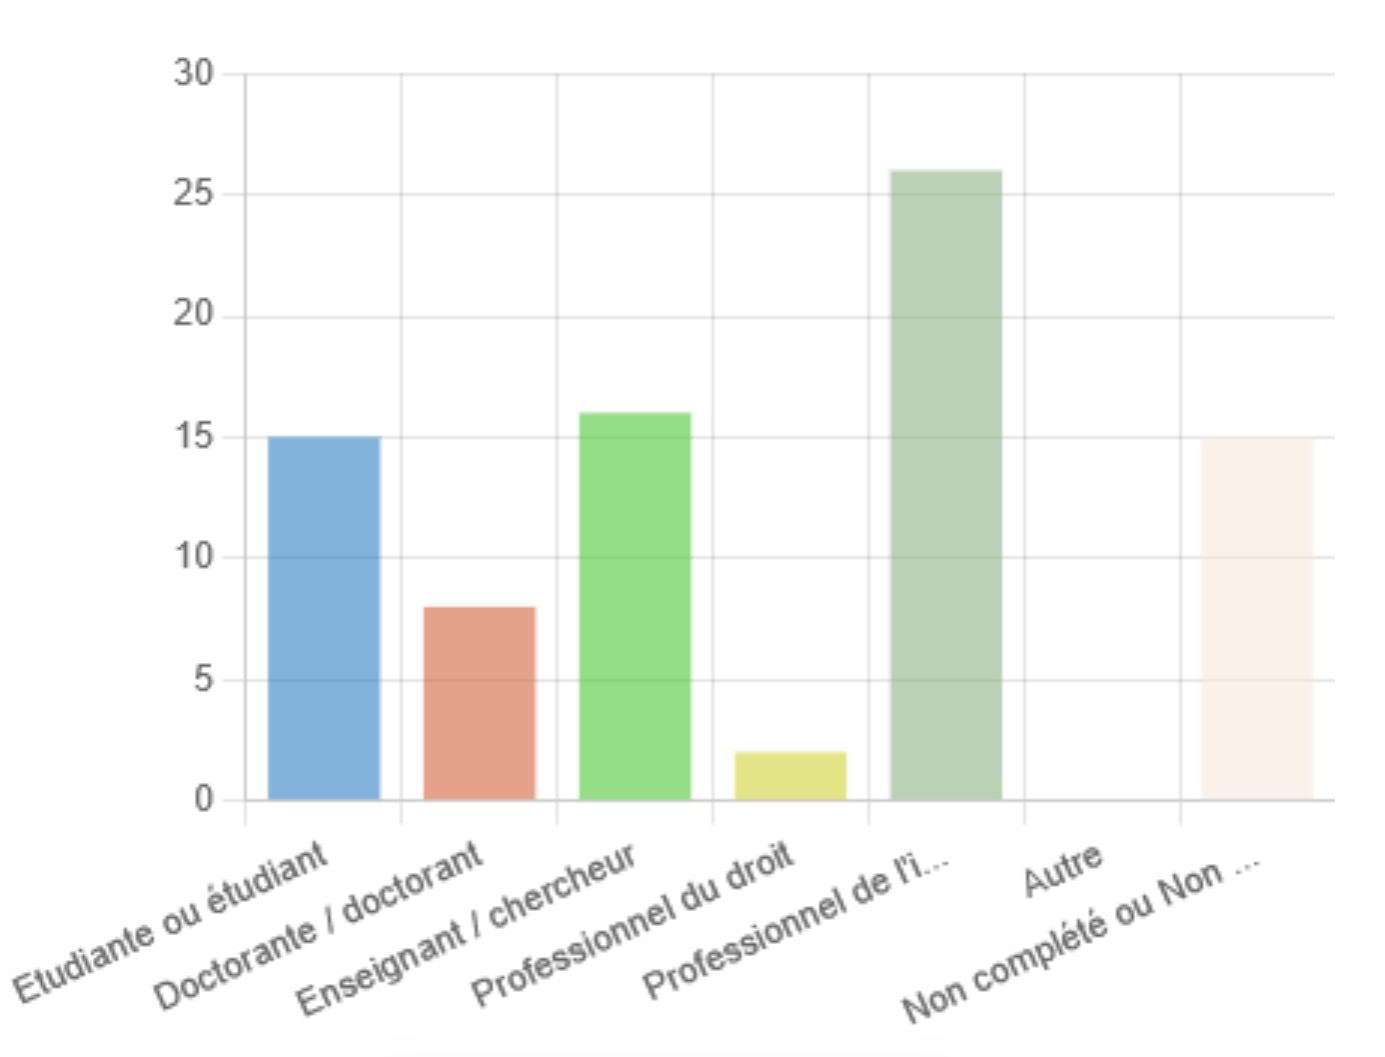
\includegraphics[width=0.5\textwidth]{./images/IMG_5952.jpeg}

Spécialité des lecteurs : 

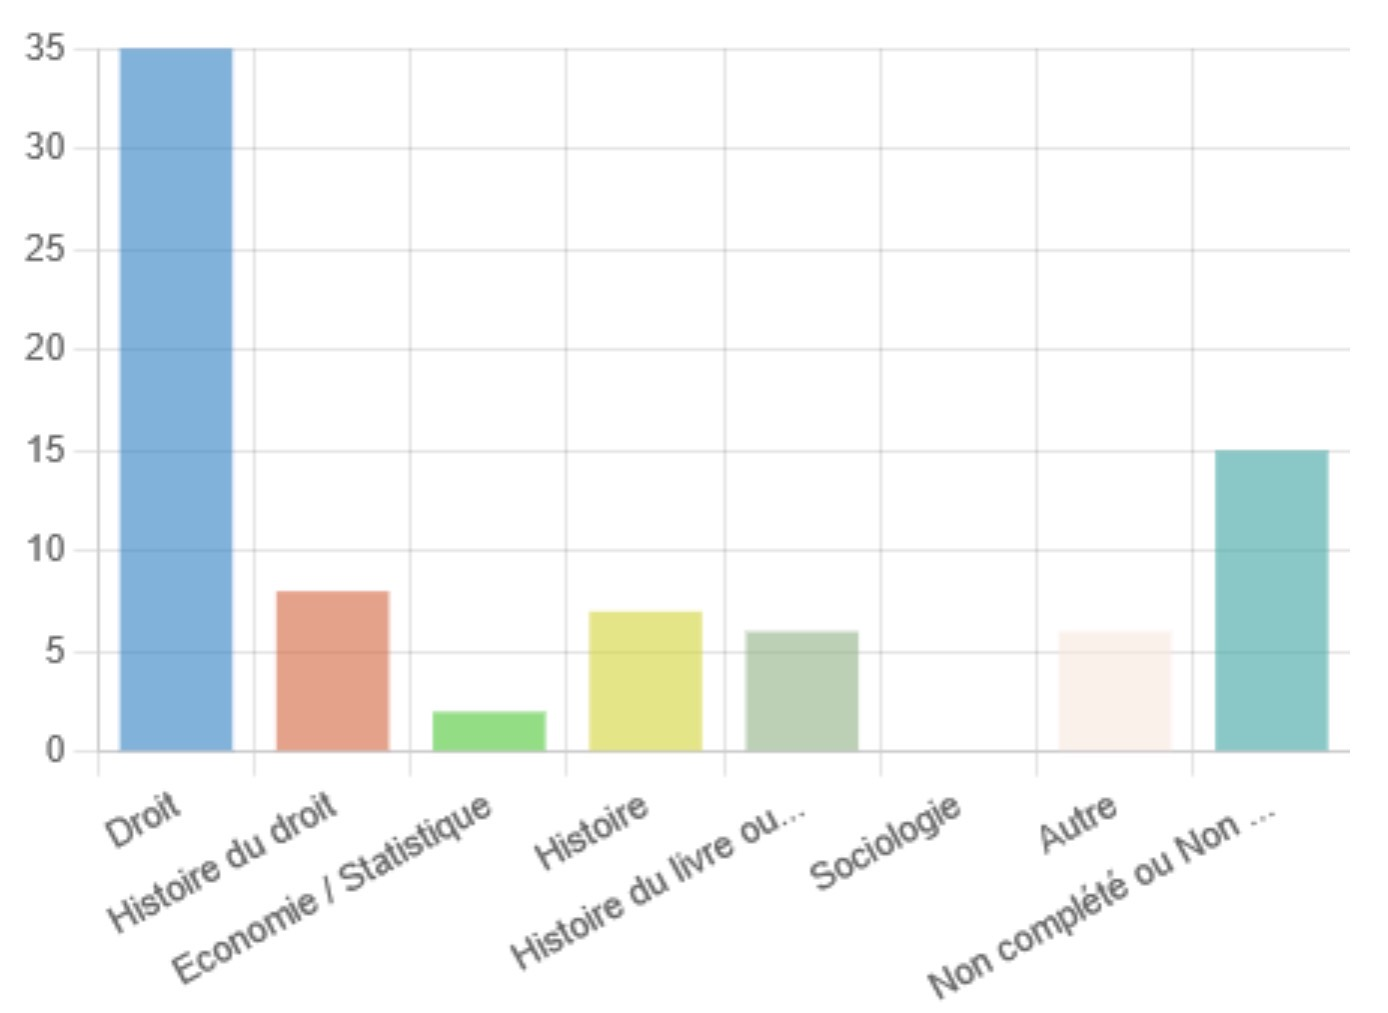
\includegraphics[width=0.5\textwidth]{./images/IMG_5953.jpeg}

Réponses aux nouveaux services ou fonctionnalités proposées :  

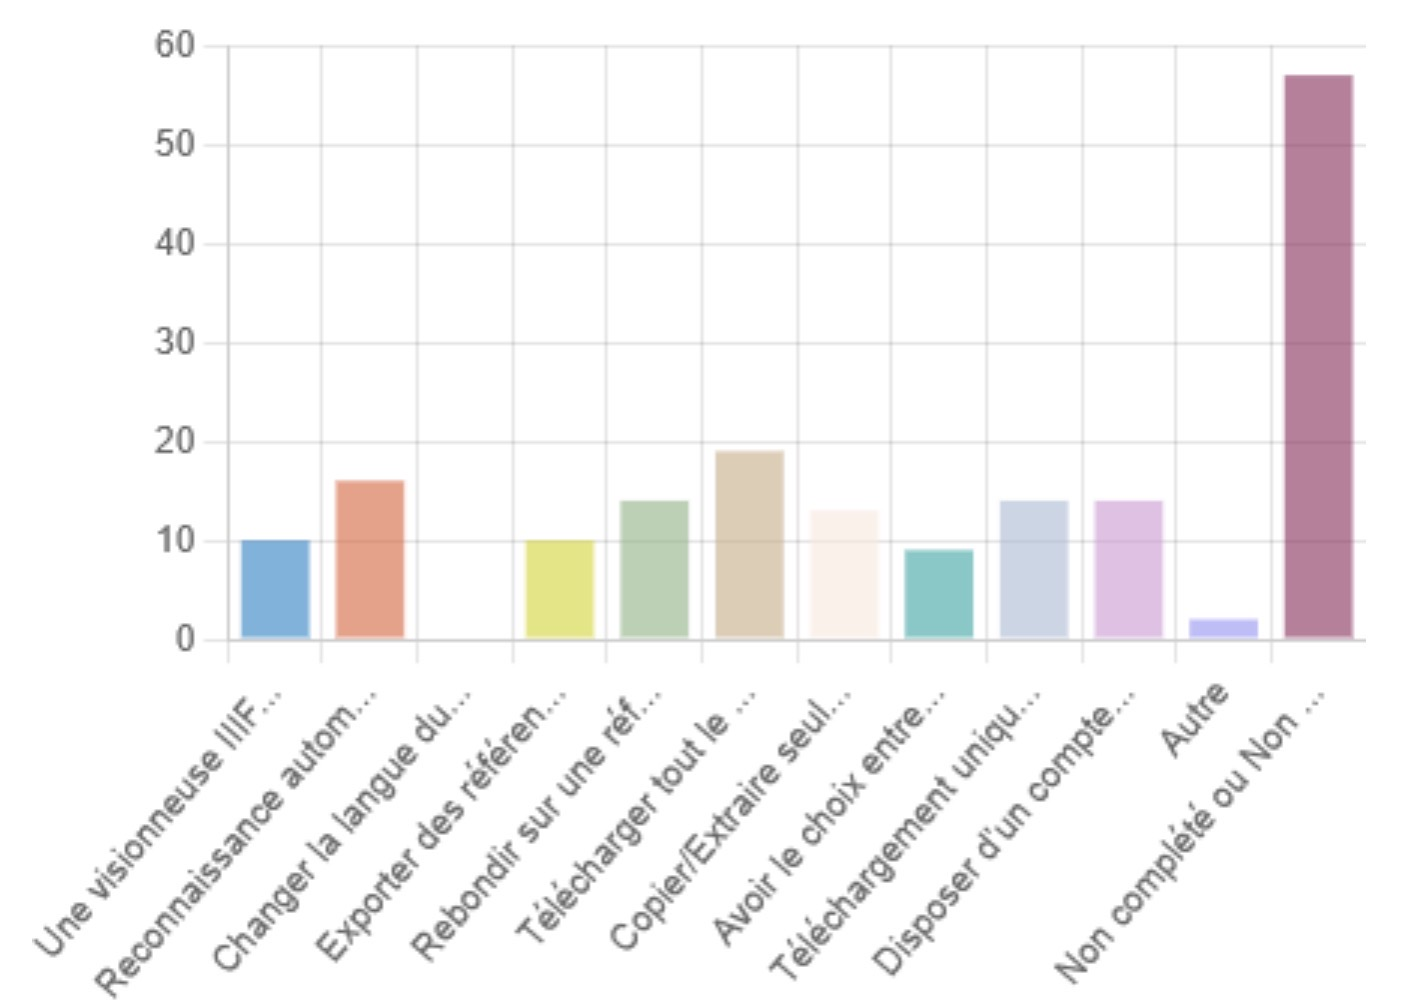
\includegraphics[width=0.5\textwidth]{./images/IMG_5954.jpeg}



% !TeX spellcheck = fr_FR
\chapter{Les préconisations pour la bibliothèque numérique}
\label{annexe_B_preconisations}

\section{Présentation}
\subsection{Contexte}
Le rapport d’audit fonctionnel de l’existant révèle que malgré sa robustesse l’ancien système XTF sous lequel CujasNum a été développé souffre de défauts d’ergonomie (multiplications des facettes, impossibilité de créer des collections, absence d’éditorialisation, etc.). Le prototype Codex semble résoudre certains problèmes identifiés dans l’ancienne bibliothèque en proposant des services (visionneuse Mirador, explorer, une page par document) auxquels on est habitués dans d’autres bibliothèques numériques. Cependant, le front-office de Codex nécessite des ajustements afin de fluidifier le parcours de l’usager. C’est sur la base de ce constat que ce document a été réalisé afin de proposer les meilleures solutions d’interface possible.

\subsection{Méthodologie de travail}
J’ai adopté une méthodologie itérative et démonstrative, pour mener à bien cette étude afin de formuler des recommandations pertinentes. Celle-ci s’articule autour des étapes suivantes :
\begin{itemize}
	\item L’exploitation de l’état des lieux : je me suis appuyé sur le document réalisé pour le rapport d’audit fonctionnel et technique, intitulé état de l’existant de la bibliothèque numérique actuelle et du prototype Codex. Ce document fait état des limites des fonctionnalités proposées dans Codex et des besoins exprimés par les utilisateurs et les professionnels. Il fait émerger les éléments essentiels à implémenter dans le nouveau système. 
\item Pour chaque thématique étudiée, ma méthode de travail fut la suivante : 
\begin{itemize}
	\item Identification des besoins
\item Réalisation d’un benchmark de cette fonction comparant ce qui se fait ailleurs, 
\item Préconisations pour le prototype Codex
\item Eventuellement proposition d’un module technique. 
\item Examen de la pertinence de la fonction proposée à travers la figure du personae. 
\end{itemize}
\item L’étude réalisée porte principalement sur les points suivants :
\begin{itemize}
	\item La page d’accueil et l’arborescence
\item Les modalités de recherche
\item La page d’un document 
\item Le compte personnel et les outils d’exploitation
\item La valorisation des collections.
\end{itemize}
\end{itemize}
 
\subsection{Les limites de l’étude}
\begin{itemize}
	\item Je ne traiterai pas les points suivants : les métadonnées, l’intégration des périodiques, archives, images et thèses ni de la question de l’IA. 
\item Les raisons pour lesquelles ces points n’ont pas été traités sont de plusieurs ordres :
\begin{itemize}
	\item Le temps limité pour mener à bien cette étude, qui a demandé une priorisation des éléments à étudier. 
\item Certains sujets doivent faire l’objet d’une étude approfondie dans un second temps. C’est par exemple le cas pour le traitement des métadonnées, qui nécessite un travail de concertation entre plusieurs services de la BIU Cujas 
\item Les autres types de documents (archives, périodiques…) n’ont pas été abordés car ils nécessitent une étude approfondie spécifique. L'objectif premier est ici de se focaliser sur la ré informatisation de l'existant de la bibliothèque numérique, qui est constituée de monographies. Bien que les enjeux liés à ces nouveaux formats aient été recueillis et pris en compte au moment des entretiens avec les usagers, ils demandent une réflexion sur la manière de les intégrer et de les présenter. 
\item L’intelligence artificielle a été elle aussi écartée. Elle représente une piste d’évolution technologique pertinente à explorer à l’avenir, son intégration n’a pas été jugée prioritaire pour la refonte.
\end{itemize}
\end{itemize}

\subsection{Conception du benchmark}
\subsubsection{Objectif du benchmark}
\begin{itemize}
	\item Identifier les bonnes pratiques des bibliothèques numériques
\item Comparer les fonctionnalités existantes avec ce qui se fait maintenant en bibliothèque numérique
\item Dégager des pistes d’amélioration pour Codex
\item Alimenter les choix fonctionnels du projet
\end{itemize}

\subsubsection{Corpus des bibliothèques numériques examinées}
\begin{itemize}
	\item Le corpus de bibliothèques numériques rassemblé pour l’étude :
\begin{itemize}
	\item NuBIS
\item Genovefa
\item Sciences Po
\item Gallica
\item Lucienne
\item Cariatide
\item Institut de France
\item Polona 
\item Cambridge Digital Library
\item Digital bodleian
\end{itemize}
\item Les raisons pour laquelle je choisis ces bibliothèques sont celles-ci : 
\begin{itemize}
	\item \textbf{NuBIS:} Bibliothèque numérique de la Bibliothèque Interuniversitaire de la Sorbonne (BIS, Université Paris I Panthéon Sorbonne) ayant fait l’objet d’une refonte très récente. Les fonctionnalités pertinentes proposées par la BIS sont l'éditorialisation sous différentes formes (billet de blog, expositions virtuelles, collections), la barre de recherche, la page à propos, la page présentant et donnant accès à chaque document, et la page d’aide.
\item \textbf{Genovefa:} La bibliothèque numérique de la Bibliothèque Sainte Geneviève (BSG, Université Sorbonne Nouvelle) propose des fonctionnalités de rebonds entre les documents et vers des sites externes de la bibliothèque numérique, la visionneuse Mirador ainsi que l'éditorialisation de leurs collections.
\item \textbf{Sciences Po:} La bibliothèque numérique de l’Institut d’Études Politiques de Paris présente du contenu en droit. Les fonctionnalités intéressantes sont la possibilité de créer un compte personnel avec deux types de visiteurs différenciés afin de proposer une consultation de documents sous droit, la page «à propos » ainsi que les pages d’actualités. 
\item \textbf{Gallica:} La bibliothèque numérique de la Bibliothèque nationale de France (BnF), est un outil de référence au niveau national. Gallica propose des collections juridiques dans son onglet « Droit » anciennement connu sous le nom « les essentiels du droit ». Elle propose aussi des fonctionnalités qui nous intéressent notamment le compte personnel, la possibilité du téléchargement à la carte, la surbrillance des mots recherchés dans la liste de résultats.
\item \textbf{Lucienne:} La bibliothèque numérique de l'Ecole normale supérieure (ENS) propose la possibilité de créer un compte personnel, une éditorialisation des collections (expositions virtuelles, parcours normalien.ne.s), ainsi que des pages d'index (notices biographiques, personnes identifiées).
\item \textbf{Cariatide:} La bibliothèque de l’Institut national d'histoire de l'art (INHA) est pertinente pour sa manière d’organiser les collections. Elle propose elle aussi un compte personnel, des notices documentaires détaillées, des collections riches et diverses (archives, dessins, estampes, imprimés …).  L'éditorialisation des collections est bien conçue. 
\item \textbf{Institut de France:} La bibliothèque numérique de l'Institut de France regroupe les données de plusieurs bibliothèques et musées.Les collections, riches, diverses et en provenance de plusieurs institutions, sont intéressantes pour leur organisation et leur mise en valeur. 
\item \textbf{Polona:} La bibliothèque numérique de la bibliothèque nationale de Pologne. Elle permet à ses utilisateurs de se créer un compte personnel permettant de créer des collections, ajouter des annotations, enregistrer tes requêtes, mettre en favoris tes documents. Elle met en avant ses documents numérisés à travers des articles ou des billets de blog rédigés par des spécialistes. Elle a également créé un accès plus scientifiques pour les chercheurs (projets scientifiques, articles de blog, notes publiques).
\item \textbf{Cambridge Digital Library:} La bibliothèque numérique de l’université de Cambridge a été sélectionnée pour son modèle pionnier d'éditorialisation scientifique. Sa visionneuse contient des tables des matières et propose la transcription et la traduction de certains documents anciens.  Elle donne accès à des documents sous droit.
\item \textbf{Digital Bodleian:} La bibliothèque numérique de l'université d'Oxford est intéressante à consulter pour comprendre ce qui se fait dans le monde anglo-saxon. Les facettes proposent un filtrage par « object type ». Les documents sont très variés (archives, musique, ouvrages, iconographies, périodiques...)  et de différentes langues.
\end{itemize}
\end{itemize}

\subsubsection{Notation des fonctionnalités examinées}
J’ai appliqué à chacune des fonctionnalités étudiées de ces bibliothèques numériques une graduation permettant d’en évaluer le bon usage : 
\begin{itemize}
	\item 0 : la fonctionnalité n’existe pas
\item 1 : la fonctionnalité existe mais elle ne fonctionne pas ou mal.
\item 2 : la fonctionnalité existe et fonctionne normalement
\item 3 : la fonctionnalité existe avec la particularité d’avoir un fonctionnement original améliorant l’expérience habituelle des utilisateurs.
\end{itemize}
\vfill

\subsection*{Tableau de comparaison des différentes fonctionnalités issus du benchmark des bibliothèques numériques}
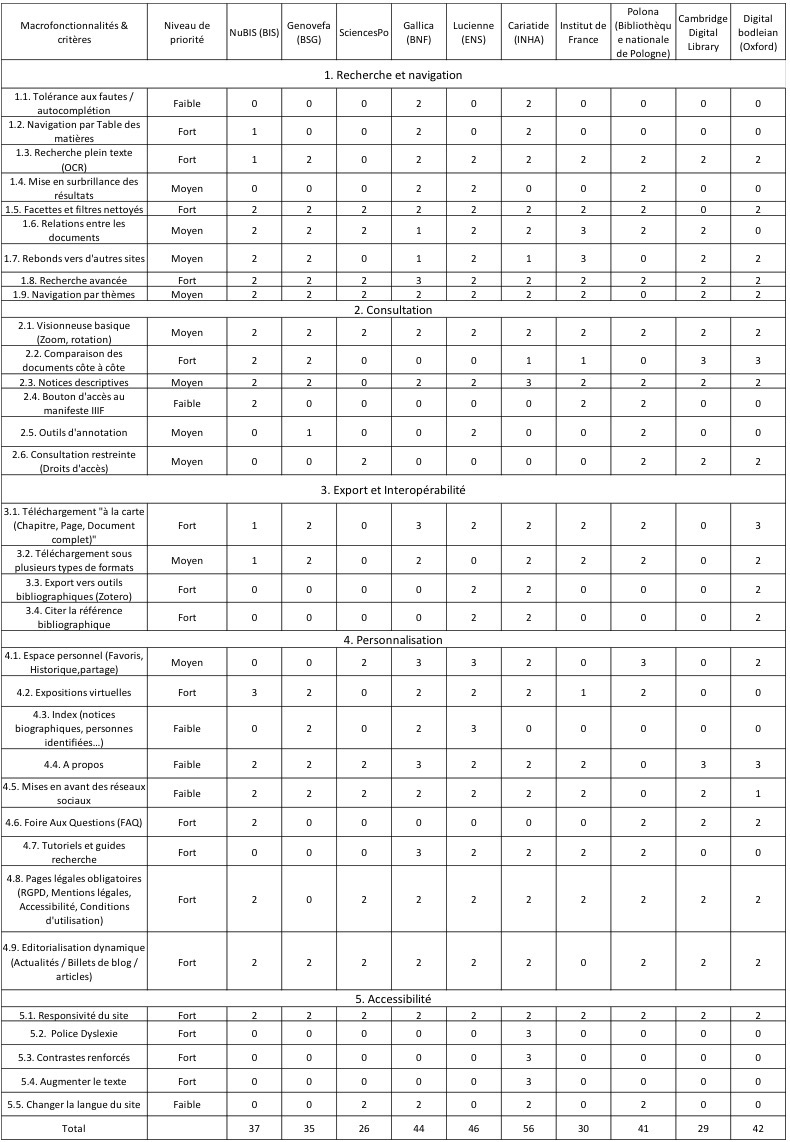
\includegraphics[width=0.9\textwidth]{./images/IMG_5955.jpeg}
\subsection{Conception des personae}
A la suite des entretiens que j’ai réalisés auprès des usagers et des différents services de Cujas, j’ai créé des personae, inspirés des informations obtenues, afin de confronter mes propositions aux besoins d’usagers types Les personae et les user stories sont des outils qui permettent de penser du point de vue des utilisateurs afin de proposer des services qui leur conviennent et d’améliorer l’expérience utilisateur.
J’ai donc réalisé six personae chacun correspondant à une catégorie d’utilisateur pouvant être amené à utiliser la bibliothèque numérique1. Les personae sont :
\begin{itemize}
	\item \textbf{Chercheur expert en histoire du droit:} il utilise la bibliothèque numérique car cela lui permet d’accéder à distance à de nombreux documents en ligne. Il apprécie d’avoir un espace centralisant les documents. Les deux fonctionnalités qu’il cherche dans une bibliothèque numérique sont les tables des matières cliquables et la recherche en plein texte. 
\item \textbf{Doctorante d’histoire du droit et des institutions:} elle utilise la bibliothèque numérique pour sa thèse. Elle trouve pratique que la table des matières soit cliquable et qu’elle ait la possibilité de pouvoir télécharger les documents qui l’intéressent sous format PDF afin de pouvoir les annoter. Elle aimerait bien que la consultation des documents numérisés se rapproche de celle des documents originaux. 
\item \textbf{Etudiant en histoire du droit:} il consulte CujasNum dans l’optique de ses recherches pour son mémoire ou dans le cadre d’exercices pratiques en cours. Il a besoin d’avoir des explications concernant la prise en main de la bibliothèque, en particulier les services proposés ou les documents que l’on trouve dans la bibliothèque.
\item \textbf{L’Amatrice éclairée:} il consulte la bibliothèque numérique pour approfondir sa culture générale ou un domaine précis. Il attend une navigation fluide, un accès direct aux sources et une médiation culturelle rigoureuse qui valorise la richesse des documents numérisés.
\item \textbf{Responsable de la bibliothèque numérique:} il est chargé de superviser le développement de la bibliothèque numérique, dans l’optique de développer un public plus varié. Il aimerait également avoir la possibilité d’ajouter d’autres types de documents ayant une architecture plus complexe. Il souhaite mettre davantage en avant la richesse des collections de sa bibliothèque. 
\item \textbf{Bibliothécaire:} elle consulte la bibliothèque numérique dans le cadre de formations et d’aide à la recherche. Elle a donc besoin d’informations claires sur le contenu, la description des documents, et des fonctionnalités de recherches fines, ainsi que des éléments explicatifs sur les modalités d’exploitation de la bibliothèque numérique.
\item \textbf{Informaticien:} il n’est pas considéré ici comme un utilisateur mais comme une personne en charge du développement et du maintien de la bibliothèque numérique.
\end{itemize}

\section[Eléments fonctionnels]{Eléments fonctionnels et techniques}
\subsection{Les modalités de recherche}
\subsubsection{Les besoins identifiés}

\begin{itemize}
	\item Recherche simple
\item Recherche avancée
\item Filtrage 
\item OCR
\item Collections
\item Filtres et facettes
\end{itemize}

\subsubsection{Benchmark}
\paragraph*{La Recherche simple:}
\addcontentsline{toc}{paragraph}{La Recherche simple:}

\textbf{Lucienne, bibliothèque numérique de l’ENS: } 
\url{https://lucienne.ens.psl.eu/s/lucienne/page/welcome}

En arrivant sur la page d’accueil, on trouve tout de suite la barre de recherche simple. Ils ont décidé de rassembler au même endroit : la recherche simple, avancée et le bouton voir (filtrage).

\begin{center}
	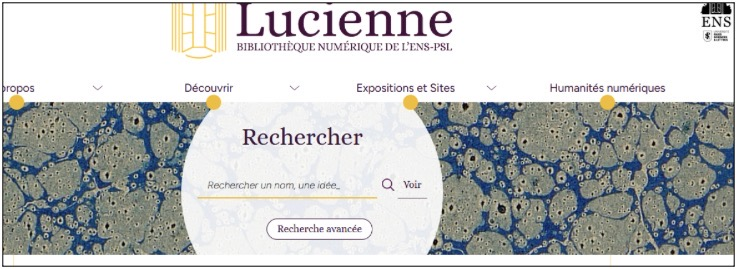
\includegraphics[width=0.7\textwidth]{./images/recherche_simple/Lucienne.jpeg}
\end{center}

\textbf{Cariatide, bibliothèque numérique de l’INHA: }
\url{https://bibliotheque-numerique.inha.fr/}

Sur la page d’accueil de Cariatide, on trouve la barre de recherche simple, avec la possibilité d’inclure ou non le plein texte et les tables des matières.

\begin{center}
	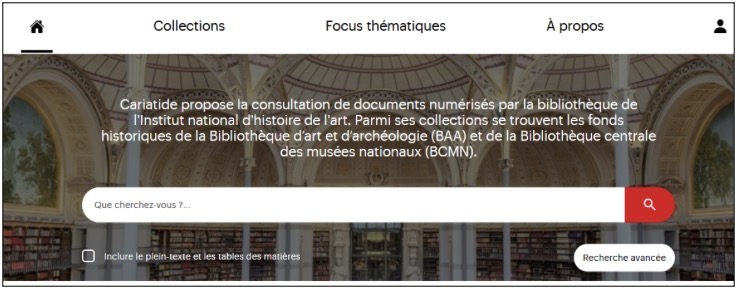
\includegraphics[width=0.7\textwidth]{./images/recherche_simple/Cariatide.jpeg}
\end{center}

\textbf{Bibliothèque numérique de l’Institut de France: } 
\url{https://bibnum.institutdefrance.fr/}

On trouve la barre de recherche sur la page d’accueil avec la possibilité de faire une recherche simple en choisissant d’inclure ou de ne pas inclure dans celle-ci le plein-texte et les sommaires et légendes.

\begin{center}
	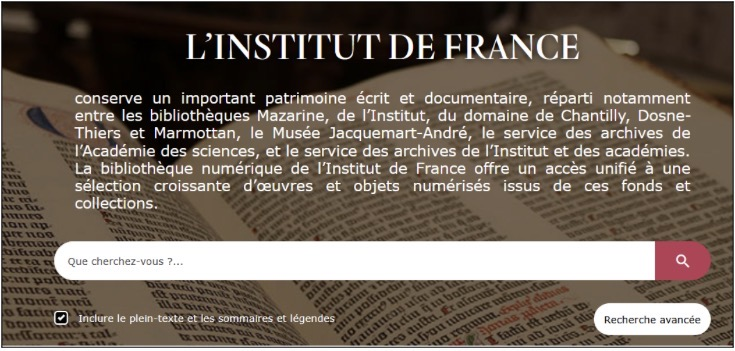
\includegraphics[width=0.7\textwidth]{./images/recherche_simple/Institut_de_France.jpeg}
\end{center}

\textbf{Gallica, bibliothèque numérique de la BNF: }
\url{https://gallica.bnf.fr/accueil/fr/html/accueil-fr}

En arrivant sur la page d’accueil, on voit directement la recherche simple matérialisée à travers cette barre de recherche. On comprend également que lorsque l’on fait une recherche, on cherche « dans les 10 millions de documents de Gallica ». 

\begin{center}
	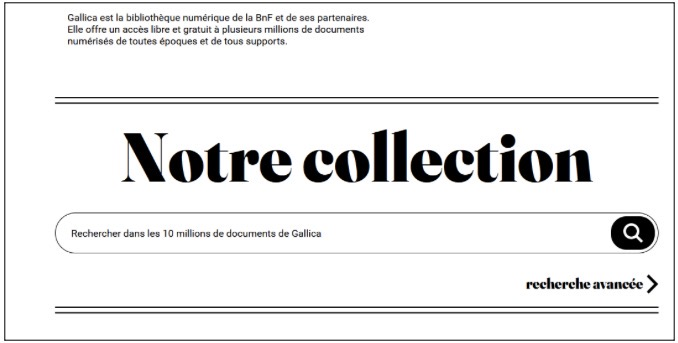
\includegraphics[width=0.7\textwidth]{./images/recherche_simple/Gallica.jpeg}
\end{center}


\textbf{NuBIS, bibliothèque numérique de la BIS: }
\url{https://nubis.bis-sorbonne.fr/}

La barre de recherche simple est présente dès la page d’accueil. Passer la souris sur la barre fait apparaitre trois options de recherche : plein texte et métadonnée, métadonnées, plein texte. A chaque fois, une courte phrase explique dans quoi la recherche est effectuée en fonction de l’option choisie.

\begin{center}
	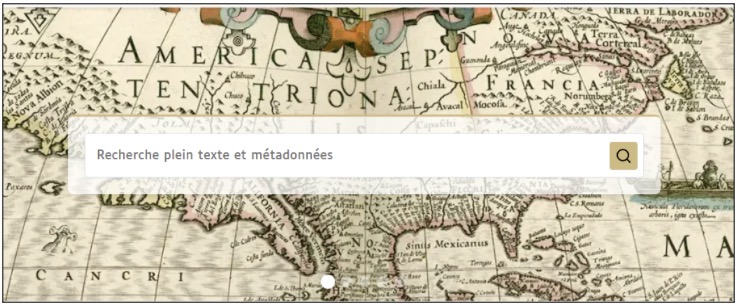
\includegraphics[width=0.7\textwidth]{./images/recherche_simple/NuBIS}
\end{center}

\paragraph*{La recherche avancée :}
\addcontentsline{toc}{paragraph}{La recherche avancée :}

\textbf{Lucienne, bibliothèque numérique de l’ENS: }
\url{https://lucienne.ens.psl.eu/s/lucienne/item/search}

La recherche avancée est accessible par un bouton dès la page d’accueil de la bibliothèque numérique, sous la barre de recherche simple. Elle consiste en un formulaire sophistiqué dans lequel l’utilisateur se voit proposer plusieurs possibilités : 
\begin{itemize}
	\item Le paramétrage du tri des références trouvées
\item Une recherche en plein texte
\item Une recherche par « filtre » permettant de chercher dans des zones spécifiques de la notice, avec des opérateurs de recherche pointus (booléens, etc.)
\item Une recherche dans une collection spécifique.
\end{itemize}

\begin{center}
	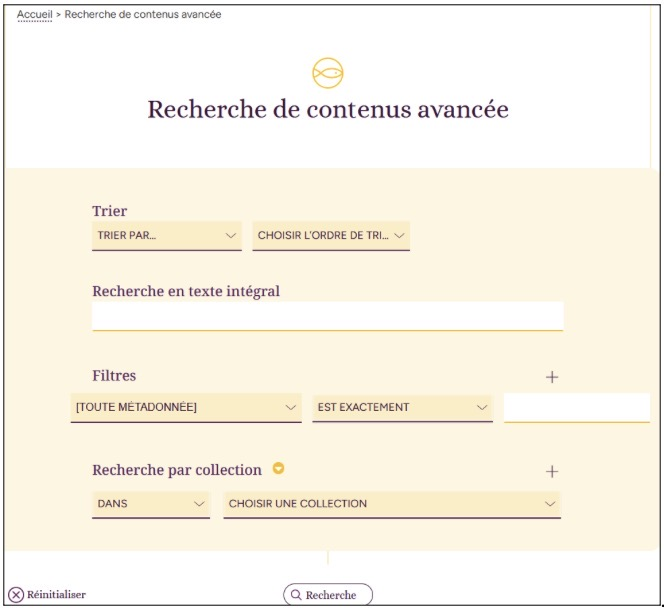
\includegraphics[width=0.7\textwidth]{./images/recherche_avancee/Lucienne.jpeg}
\end{center}

\textbf{Bibliothèque numérique de l’institut de France et des académies: } 
\url{https://bibnum.institutdefrance.fr/recherche-avancee?}

En cliquant sur le bouton de recherche avancée présent sur la page, celui-ci nous amène à un formulaire de recherche. Il permet de sélectionner les éléments dans lesquels on cherche (zones de la notice, plein texte, sommaires et légendes) et d’utiliser les opérateurs booléens ET, OU et SAUF. 

\begin{center}
	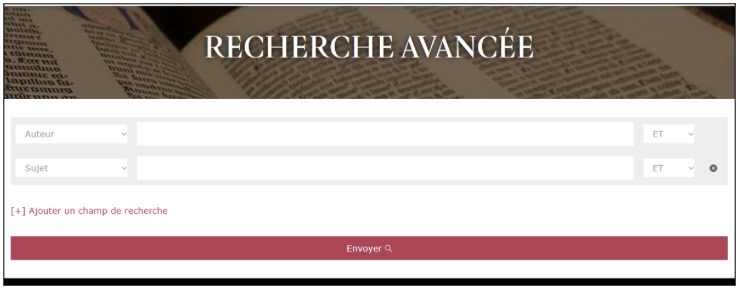
\includegraphics[width=0.7\textwidth]{./images/recherche_avancee/Institut_de_France.jpeg}
\end{center}

\textbf{Cariatide, bibliothèque numérique de l’INHA: }
\url{https://bibliotheque-numerique.inha.fr/recherche-avancee}

La recherche avancée se trouve sur la page d’accueil amenant à un formulaire de recherche. Celui-ci permet de sélectionner les données dans lesquelles on cherche (zones de la notice, plein texte, table des matières) et d’ajouter un champ de recherche.

\begin{center}
	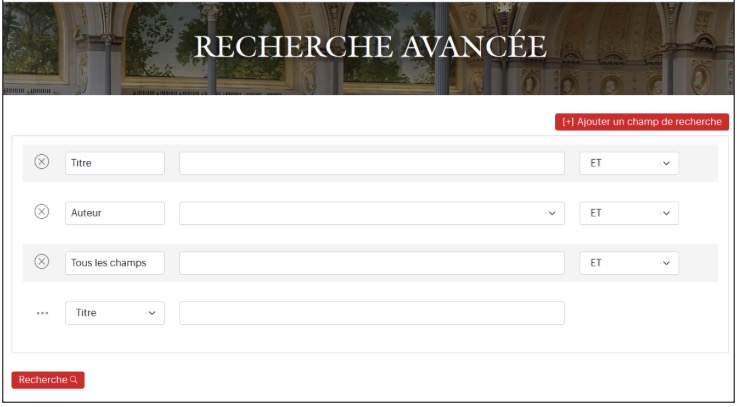
\includegraphics[width=0.7\textwidth]{./images/recherche_avancee/Cariatide.jpeg}
\end{center}

\textbf{Gallica, bibliothèque numérique de la BNF: }
\url{https://gallica.bnf.fr/services/engine/search/advancedSearch/}

La recherche avancée est présente sous forme d’un lien cliquable dès la page d’accueil. Le formulaire de recherche avancée. On remarque qu’il y a différentes catégories de recherche en plus de la recherche en texte intégral. Un filtrage par type de document est proposé, ainsi qu’une recherche par proximité de termes. Il est possible de filtrer par bibliothèque versante et par collection ou thème. 

\begin{center}
	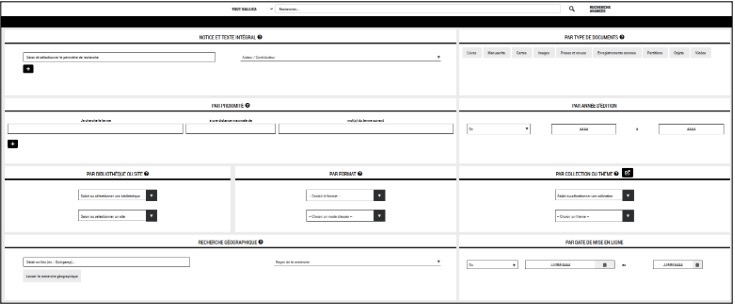
\includegraphics[width=0.7\textwidth]{./images/recherche_avancee/Gallica.jpeg}
\end{center}

\textbf{Polona, bibliothèque numérique de la bibliothèque nationale de Pologne: }
\url{https://polona.pl/} 

Le formulaire de recherche avancée permet de faire un filtrage par droit d’auteur.

\begin{center}
	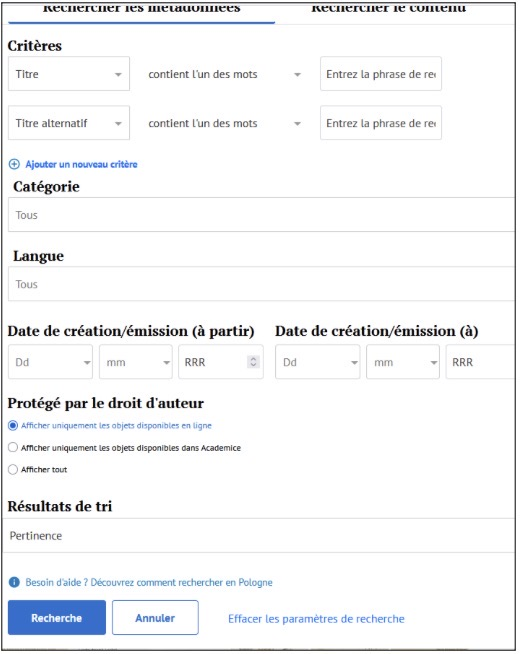
\includegraphics[width=0.5\textwidth]{./images/recherche_avancee/Polona.jpeg}
\end{center}

\paragraph*{Recherche par filtrage (filtres, facettes):}
\addcontentsline{toc}{paragraph}{Recherche par filtrage (filtres, facettes):}
Il s’agit de la recherche par filtrage intitulée « Explorer » dans le prototype Codex, qui comprend l’ensemble des documents que l’on peut filtrer par des facettes. 

\begin{center}
	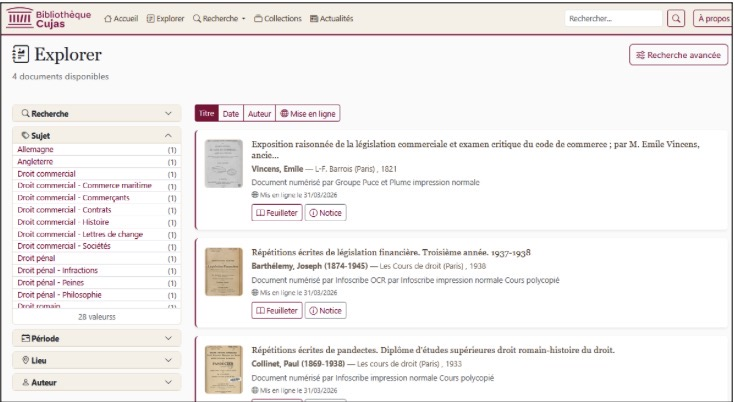
\includegraphics[width=0.5\textwidth]{./images/filtrage/IMG_5966.jpeg}
\end{center}

\textbf{Cariatide, bibliothèque de l’INHA:}
\url{https://bibliotheque-numerique.inha.fr/collection/?search=&sort=_score&perpage=10&}

Cariatide permet d’activer simultanément plusieurs filtres. Les filtres utilisés s’affichent au-dessus de la barre de recherche : on sait donc exactement quel filtre a été pris en compte.

\begin{center}
	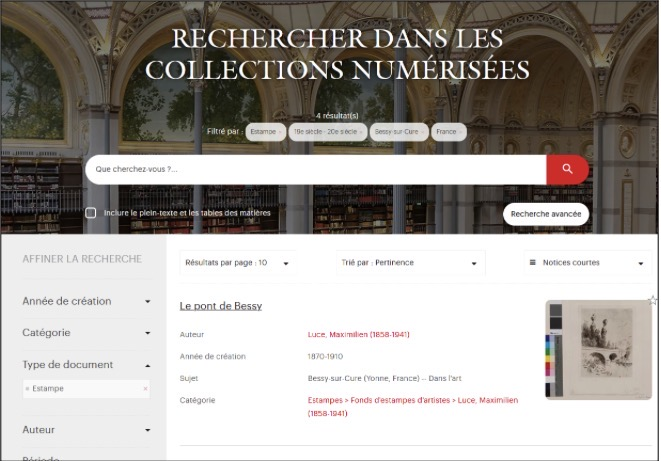
\includegraphics[width=0.5\textwidth]{./images/filtrage/IMG_5967.jpeg}
\end{center}

\url{https://bibliotheque-numerique.inha.fr/collection/?search=&sort=_score&perpage=10&page=1&&refine[Type][]=Estampe&r&&refine[period][]=19e+si%C3%A8cle+-+20e+si%C3%A8cle&r&&refine[locationcity][]=Bessy-sur-Cure&r&date_field=Date&&page=1&refine[locationcountry][]=France#title}

\textbf{Genovefa, Bibliothèque Sainte Geneviève}
\url{https://genovefa.bsg.univ-paris3.fr/s/genovefa/recherche}

La BSG propose un système de filtres particulièrement détaillé, catégorisé en fonction de ce que l’on souhaite rechercher (type, auteur, éditeur).

\begin{center}
	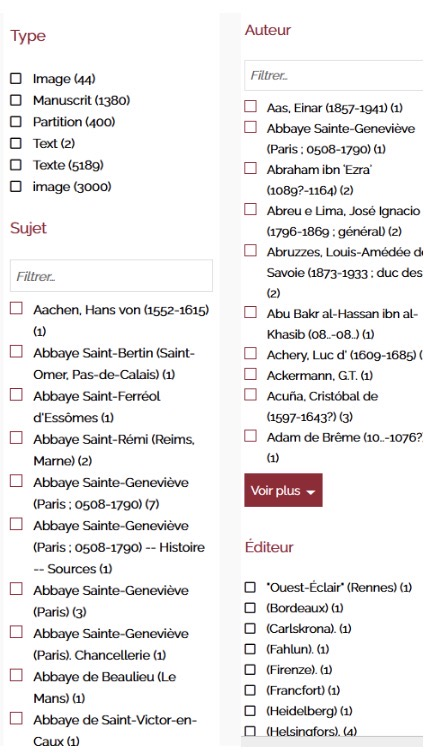
\includegraphics[width=0.5\textwidth]{./images/filtrage/IMG_5968.jpeg}
\end{center}

\textbf{NuBIS, bibliothèque numérique de la BIS}
\url{https://nubis.bis-sorbonne.fr/search?}

Dans sa recherche par filtrage, NuBIS a fait le choix de proposer plusieurs types de filtres qui s’appliquent à tous les documents, quelque-soit leur type.

\begin{center}
	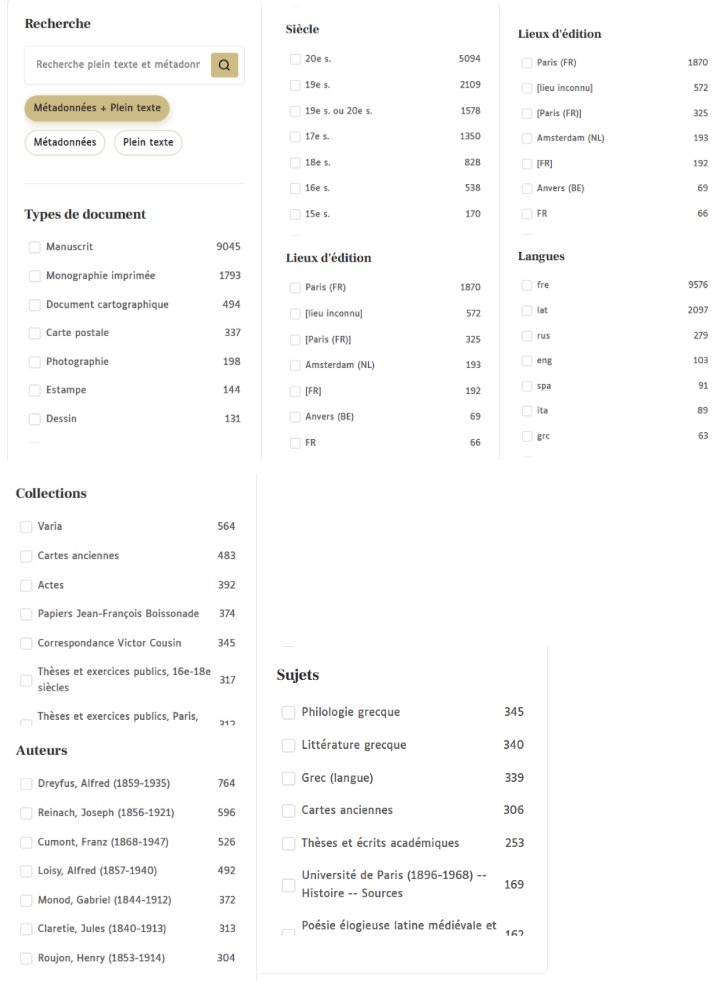
\includegraphics[width=0.5\textwidth]{./images/filtrage/IMG_5969.jpeg}
\end{center}

\textbf{Polona, bibliothèque numérique de la bibliothèque nationale de Pologne:}
\url{https://polona.pl/public-collections/collection/0de5caee-dd56-4e16-acc6-df73c5b1df4b}

Les filtres de Polona sont intéressant surtout pour la création des filtres concernant les droits (protégé par le droit d’auteur, droits sur l’œuvre, licence).

\begin{center}
	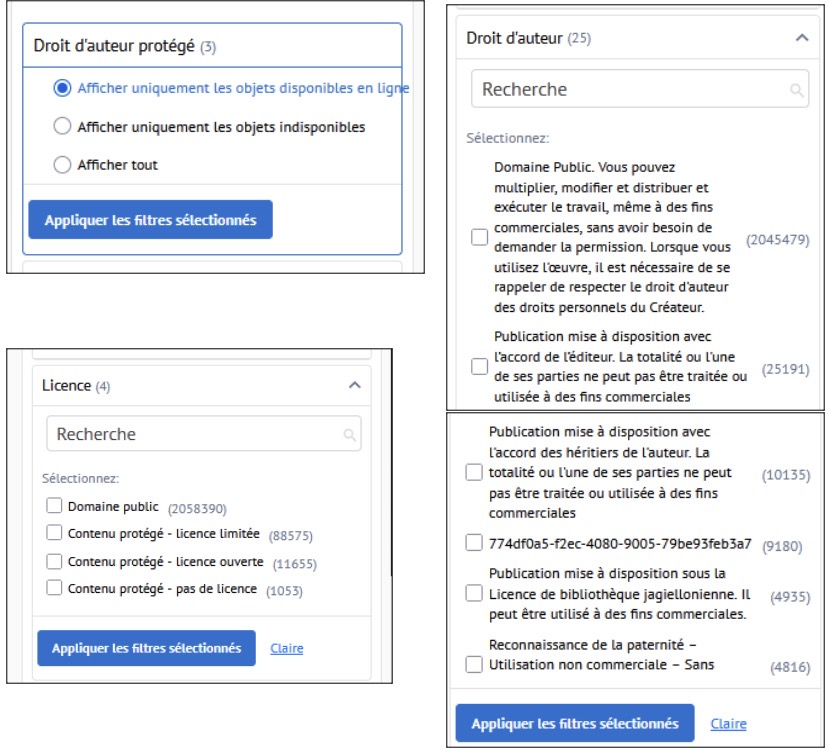
\includegraphics[width=0.5\textwidth]{./images/filtrage/IMG_5970.jpeg}
\end{center}

\textbf{Bodleian Library, bibliothèque numérique d’Oxford:}
\url{https://digital.bodleian.ox.ac.uk/search/#s=advanced}

Les filtres de la Digital Library permettent de filtrer les documents océrisés (filtre Has Text), les documents partiellement ou totalement numérisés (fully digitized). Elle propose des collections (collection) qui correspondent à des types de documents, ainsi que des corpus thématiques (Project). 

\begin{center}
	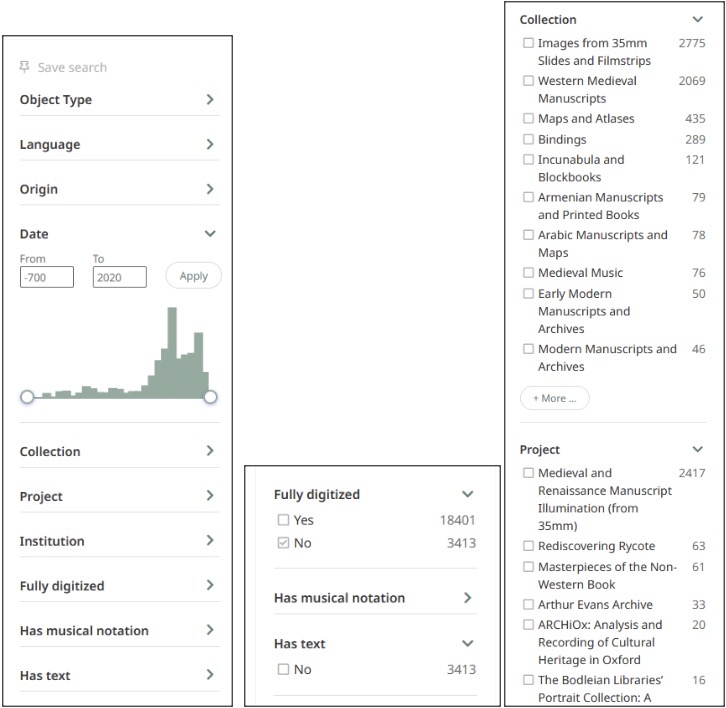
\includegraphics[width=0.5\textwidth]{./images/filtrage/IMG_5971.jpeg}
\end{center}

\paragraph*{Collections:}
\addcontentsline{toc}{paragraph}{Collections:}
\textbf{NuBIS, bibliothèque numérique de la BIS: }
\url{https://nubis.bis-sorbonne.fr/collections}

La BIS a fait le choix de présenter ces collections sous la forme de vignette indiquant également s’il y a une exposition sur le sujet ou bien des sous-collections avec le nombre précis à chaque fois.

\begin{center}
	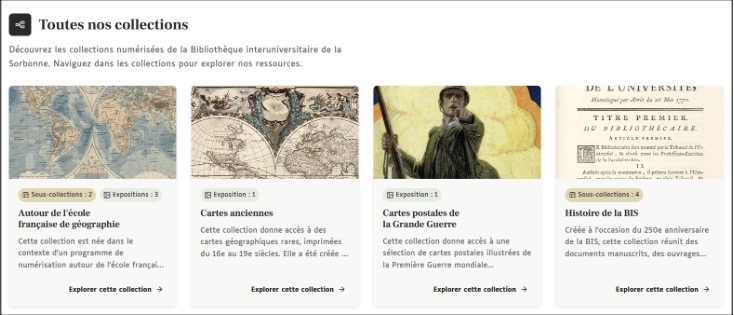
\includegraphics[width=0.5\textwidth]{./images/collections/IMG_5972.jpeg}
\end{center}

\textbf{Cariatide, bibliothèque numérique de l’INHA:}
\url{https://bibliotheque-numerique.inha.fr/}

Sur la page d’accueil de Cariatide, il est possible de trouver les six collections numérisées de la bibliothèque. En cliquant dessus, on arrive sur la collection en elle-même avec une présentation des sous-collection sommaires sous forme de table des matières. En bas de page, un bouton est présent permettant de faire une recherche simple ou par filtres uniquement dans la collection numérisée choisie. 

\begin{center}
	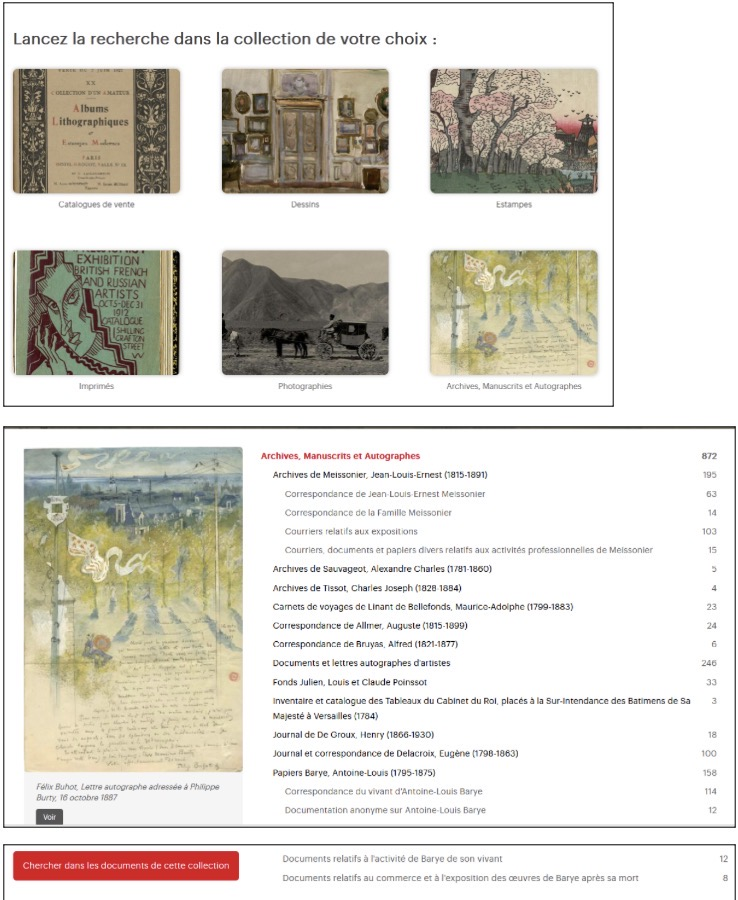
\includegraphics[width=0.5\textwidth]{./images/collections/IMG_5973.jpeg}
\end{center}

\textbf{Lucienne, bibliothèque numérique de l’ENS: }
\url{https://lucienne.ens.psl.eu/s/lucienne/page/collections}

L’ENS a fait le choix de présenter ses collections sous une classification typologique. La page Collections affiche une sélection de six collections. Un bouton « Découvrir toutes les collections » permet d’afficher l’ensemble des collections.

\begin{center}
	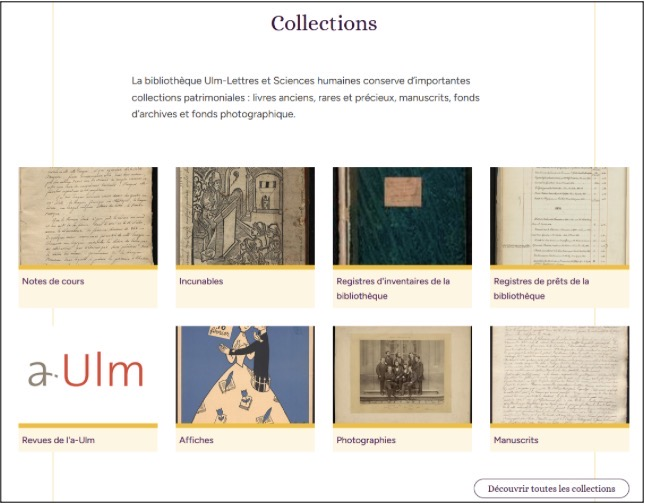
\includegraphics[width=0.5\textwidth]{./images/collections/IMG_5974.jpeg}
\end{center}

\textbf{Bibliothèque numérique de l’institut de France et des académies: }
\url{https://bibnum.institutdefrance.fr/corpus-parcours}

L’onglet « Corpus et parcours » présente les collections numérisées de l’Institut de France et des académies qui lui sont rattachées en deux ensembles : 
\begin{itemize}
	\item Un ensemble de collections classées par typologie (iconographie \& illustration, imprimés, …)
\item Un ensemble de collections classées par corpus ou par parcours thématiques.
\end{itemize} 
L’institut a fait le choix de les présenter sous la forme de vignettes. 

\begin{center}
	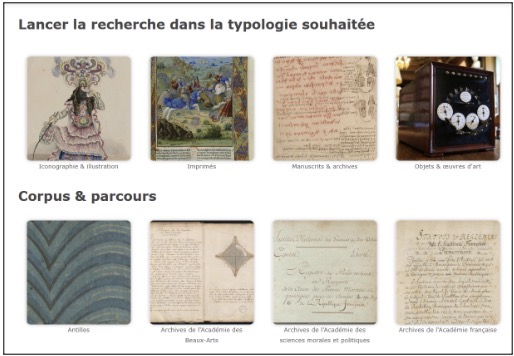
\includegraphics[width=0.5\textwidth]{./images/collections/IMG_5975.jpeg}
\end{center}

\textbf{Polona, bibliothèque numérique de la bibliothèque nationale de Pologne: }
\url{https://polona.pl/}

La page d’accueil affiche les collections en accès publique sur la bibliothèque numérique. Les collections sont organisées de façon thématique.

\begin{center}
	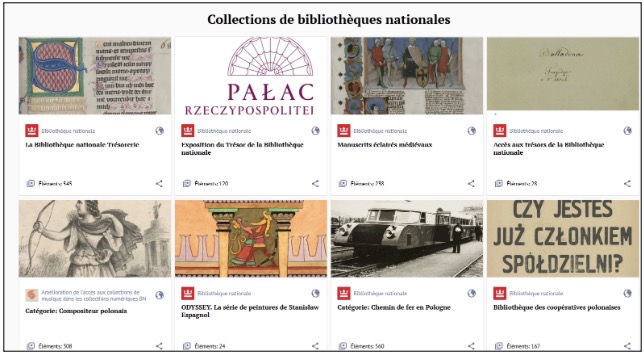
\includegraphics[width=0.5\textwidth]{./images/collections/IMG_5976.jpeg}
\end{center}

\textbf{Digital Bodleian, bibliothèque numérique d’Oxford: }
\url{https://digital.bodleian.ox.ac.uk/browse/}

L’université d’Oxford présente ses collections suivant une arborescence hybride qui combine des critères géographies, temporels et matériels.

\begin{center}
	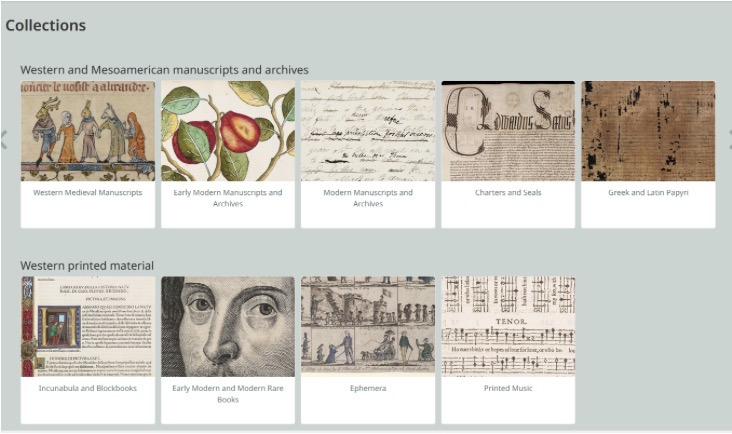
\includegraphics[width=0.5\textwidth]{./images/collections/IMG_5977.jpeg}
\end{center}

\subsubsection{Proposition pour la bibliothèque numérique de Cujas}

\begin{itemize}
	\item \uline{Recherche simple:} la barre de recherche doit être présente sur la page d’accueil au centre avoir la possibilité de choisir d’inclure la recherche dans les métadonnées, le plein-texte et les métadonnées et le plein-texte. 
\item \uline{Recherche avancée:} il faut qu’il y est un bouton cliquable se trouvant en-dessous de la barre de recherche amenant à un formulaire de recherche. Le formulaire de recherche peut comporter les champs suivants (titre, auteur, sujet, date de début et de fin, lieu et la classification Dewey).
\item \uline{Recherche par filtrage:} l’ajouter comme un onglet séparé des autres formes de recherche afin de différencier leurs utilisations. On peut la représenter par la rubrique \enquote{Explorer} avec une loupe qui l’accompagne. Les filtres peuvent contenir les champs suivants : type de documents, sujets, auteurs, siècles, langues, éditeurs, les droits, les collections). Les filtres actionnés doivent être clairement identifiés (affichés en haut de la page ou signalés par une mise en couleur, par exemple).
\item Présenter les collections sous formes de vignettes en indiquant le nombre de sous-collections constituant celle-ci. 
\end{itemize}

\subsubsection{Eléments techniques}

\paragraph*{Module Advanced Search (Omeka.org)}
\addcontentsline{toc}{paragraph}{Module Advanced Search (Omeka.org)}

Lien vers la documentation:\url{https://omeka.org/s/modules/AdvancedSearch/}

Advanced Search : améliore la recherche standard (visibilité, vignettes, commence par, ressources sans modèles, recherche dans plusieurs propriétés à la fois, etc.) et permet d’ajouter d’autres capacités de recherches (autocomplétion, filtres, facettes et l’interrogation de camp agrégés). Un des adaptateurs disponibles est avec le moteur de recherche Solr.

\paragraph*{API Omeka-S-module-SearchSolr}
\addcontentsline{toc}{paragraph}{API Omeka-S-module-SearchSolr}

Lien vers la documentation:\url{https://github.com/Daniel-KM/Omeka-S-module-SearchSolr}
 
API pour se connecter au moteur de recherche Solr (différent du module développé par Biblivre).
Module basé sur la bibliothèque Solarium. Il est livré avec une API et une documentation complète, permettant d’intégrer de nouvelles fonctionnalités pour l’indexation et l’interrogation. 
Moteur de recherche Solr (Apache Solr: \url{https://solr.apache.org/}): plateforme de recherche multimodale ultra-rapide, open source construite sur le texte intégral, le vecteur et les capacités de recherche géospatiale d’Apache Lucene. Modèle fiable, évolutif et tolérant aux pannes, fournissant une indexation distribuée, etc. Solr alimente les fonctionnalités de recherche et de navigation.

\subsubsection{Réponse aux besoins identifiés par les personae}

Afin de valider la pertinence des choix fonctionnels proposés pour les modalités de recherche, la synthèse ci-dessous illustre comment chaque fonctionnalité répond aux besoins prioritaires des personae :
\begin{itemize}
	\item \textbf{Besoin n°1 : Accès rapide aux documents numérisés}
\begin{itemize}
	\item \uline{Personae concernés :} chercheur expert en histoire du droit, doctorante, étudiant et la bibliothécaire.
\item \uline{Réponse :} Mise en place d’une recherche simple avec autocomplétion et des filtres applicables à différents types de documents. 
\end{itemize}
\item \textbf{Besoin n°2 : Recherche croisée et ciblée dans les métadonnées :} 
\begin{itemize}
	\item \uline{Personae concernés :} chercheur expert en histoire du droit, doctorante, étudiant, l’amatrice éclairée et la bibliothécaire.
\item \uline{Réponse :} Mise en place d’un accès direct vers un formulaire de recherche avancée permettant de combiner plusieurs champs (auteur, titre, date, sujet, cote) grâce à des opérateurs logiques.
\end{itemize}
\item \textbf{Besoin n°3 : Affinement et filtrage dynamique des résultats de recherche :}
\begin{itemize}
	\item \uline{Personae concernés :} chercheur expert en histoire du droit, doctorante, étudiant, bibliothécaire et le responsable de la bibliothèque numérique. 
\item \uline{Réponse :} Mise en place de filtre permettant de sélectionner le type de document, le sujet, l’auteur, l’éditeur, le lieu, la période, les droits d’accès avec une mise en évidence dans filtres sélectionnés en haut de page dans une autre couleur.
\end{itemize}
\item \textbf{Besoin n°4 : navigation par thème}
\begin{itemize}
	\item \uline{Personae concernés :} chercheur expert en histoire du droit, doctorante, étudiant.
\item \uline{Réponse :} Présentation des collections sous formes de vignettes avec une image et des titres explicites avec une indication des sous-collections la constituant.

\end{itemize}
\end{itemize}

\subsection{La page d’un document}
\subsubsection{Les besoins identifiés}
\begin{itemize}
	\item Une page descriptive par document numérisé
\item Visionneuse Mirador
\item  Rebonds à l’intérieur de la bibliothèque numérique mais également à l’extérieur de celle-ci
\item Citation du document
\item Exportation des données sous différents formats
\end{itemize}

\subsubsection{Benchmark}
\textbf{Cariatide, bibliothèque numérique de l’INHA:} 
\url{https://bibliotheque-numerique.inha.fr/collection/item/30452-dessins-de-costumes-par-berain-pour-des-pieces-de-lully?offset=1#item_data_title}
\begin{itemize}
	\item Une notice très détaillée. On comprend très bien tous les éléments constituant la notice. Celle-ci est divisée en plusieurs parties. Par contre le titre qui ne se distingue pas particulièrement du reste de la notice pouvant amener à s’interroger afin de savoir où il se trouve.
\item Des rebonds depuis les noms de personnes, les types de documents, les focus thématiques. 
\item Le bloc « Réutiliser », qui cite la bibliothèque d’origine, les conditions d’utilisation (lien vers des précisions) et donne le lien vers le Manifeste IIIF. 
\item Un bouton de copie du permalien
\item Une citation du document copiable
\end{itemize}

\begin{center}
	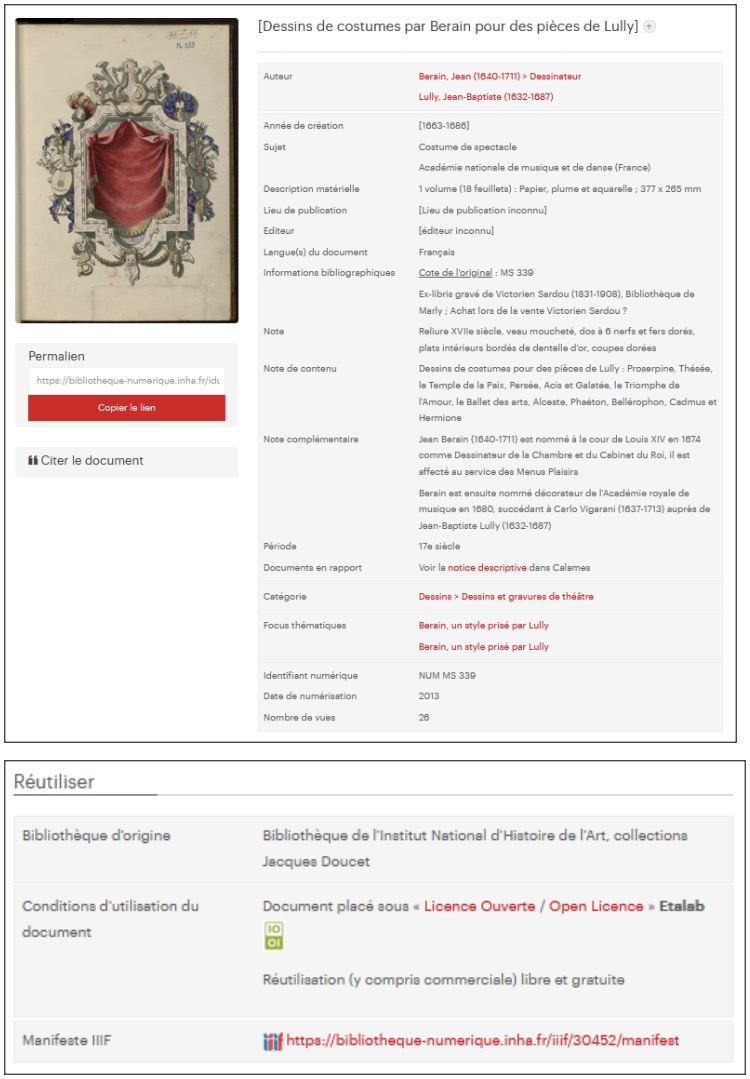
\includegraphics[width=0.6\textwidth]{./images/page_document/IMG_5978.jpeg}
\end{center}


\textbf{NuBIS, bibliothèque numérique de la BIS:}

\url{https://nubis.bis-sorbonne.fr/ark:/15733/qcmq?view=full}
\begin{itemize}
	\item On voit en haut de quelle collection est issu le document. 
\item Outils d’exploitation regroupés en haut de la page (Permalien, Manifest IIIF, Licence)
\item Le type de licence est clairement indiqué en haut. Il s’agit d’un lien qui renvoie sur une page détaillée décrivant la licence
\item Rebonds depuis les noms de personnes
\item Lien vers le catalogue décrivant le document 
\item Notice succincte en haut de page que l’on peut déployer
\end{itemize}

\begin{center}
	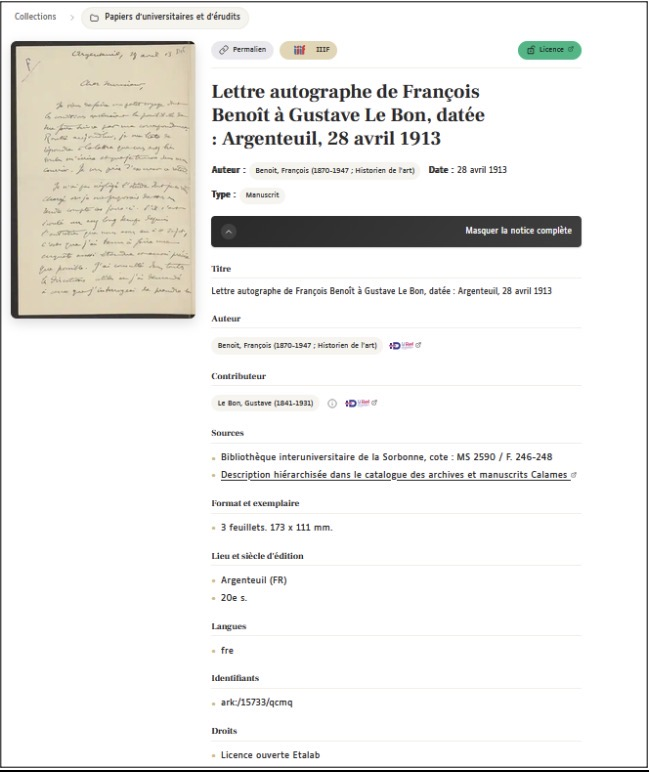
\includegraphics[width=0.6\textwidth]{./images/page_document/IMG_5979.jpeg}
\end{center}

\textbf{Lucienne, bibliothèque numérique de l’ENS:}

\url{https://lucienne.ens.psl.eu/s/lucienne/item/51543}
Les pages de présentation des documents de Lucienne sont intéressantes pour : 
\begin{itemize}
	\item La présence d’un fil d’ariane
\item Une référence succincte en haut de la page, complétée de la notice complète plus bas. 
\item Une notice comprenant la collection, le lien vers la notice dans le catalogue d’origine, et le signalement d’entités nommées. 
\item De nombreux rebonds
\item La possibilité de copier une citation. 
\item La possibilité d’exporter les données sous différents formats (BibTex, CSV, Json-Table).
\end{itemize}
Par contre, la présentation en colonne, y compris sur grand écran, nécessite une manipulation de la souris fastidieuse. 

\begin{center}
	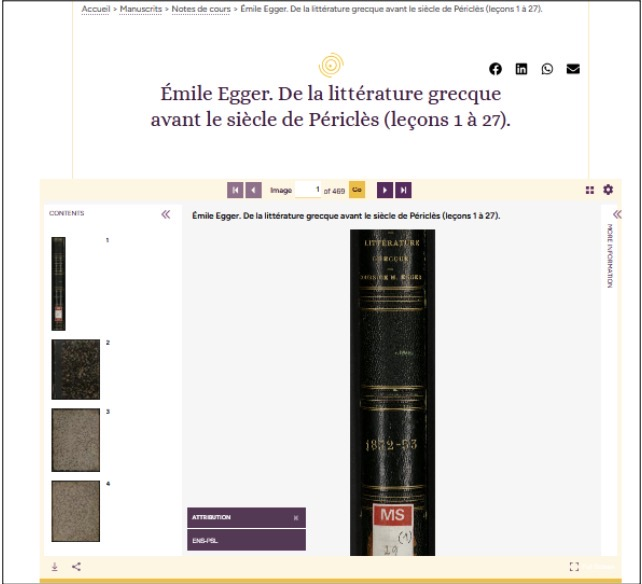
\includegraphics[width=0.6\textwidth]{./images/page_document/IMG_5980.jpeg}
	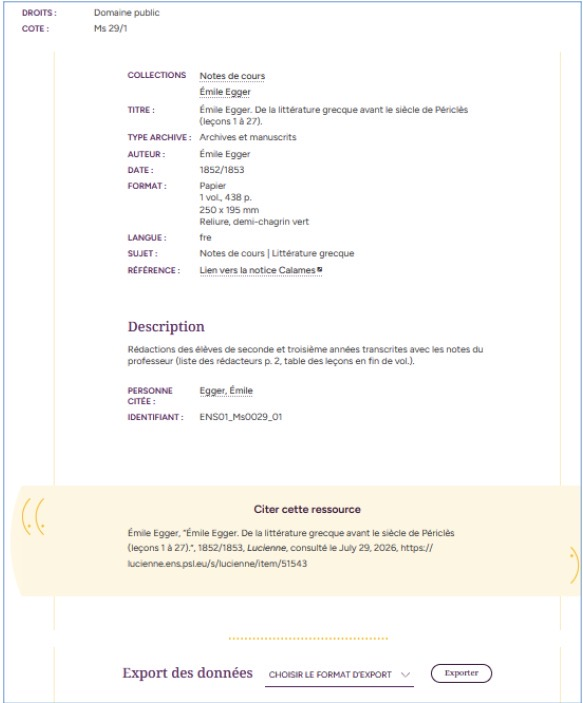
\includegraphics[width=0.6\textwidth]{./images/page_document/IMG_5981.jpeg}
\end{center}

\subsubsection{Proposition pour la bibliothèque numérique de Cujas}
\begin{itemize}
	\item Une notice succincte avec la possibilité de masquer ou dérouler une notice complète 
\item  Le document sur la gauche, en position sticky (l’image reste fixe y compris lorsqu’on fait dérouler la partie droite de l’écran) et la notice à droite que l’on peut faire défiler à l’écran.
\item Le manifeste IIIF disponible sous forme de bouton sur la page de présentation, en plus de celui que l’on peut trouver dans la visionneuse Mirador.
\item Conserver la vignette cliquable amenant directement sur la visionneuse.
\end{itemize}

\subsubsection{Eléments techniques}

\paragraph*{Module Bibliography (Omeka-S)}

\url{https://github.com/Daniel-KM/Omeka-S-module-Bibliography}
Le module Bibliography d’Omeka S est utile pour générer et gérer des citations bibliographiques standardisées, afficher des blocs de références sur les pages publiques d’un site et importer des notices via des identifiants (comme le DOI ou l’ISBN).

\paragraph*{Module CopyIdRef (Omeka-S)}

\url{https://omeka.org/s/modules/CopIdRef/}

Le module Copy IdRef permet d’utiliser le thésaurus IdRef de l’ABES. Il permet de générer automatique une page de présentation de l’auteur et liste tous les autres documents du catalogue lié à cet auteur. 


\subsubsection{Réponse aux besoins identifiés par les personae}
Afin de valider la pertinence des choix fonctionnels proposés pour la page d’un document, la synthèse ci-dessous illustre comment chaque fonctionnalité répond aux besoins prioritaires des personae :
\begin{itemize}
	\item \textbf{Besoin n°1 : Description détaillée d’un document}
\begin{itemize}
	\item \uline{Personae concernés :} chercheur expert en histoire du droit, doctorante, étudiant, amatrice éclairée, bibliothécaire et responsable de la bibliothèque numérique.
\item \uline{Réponse :} Une notice détaillée avec le titre, le type de document et l’auteur mis en évidence avec le reste de la notice présenté dans un menu déroulant accompagné du manifeste IIIF présenté sous la forme d’un bouton.
\end{itemize} 
\item \textbf{Besoin n°2 : Exporter la référence de la ressource}
\begin{itemize}
	\item \uline{Personae concernés :} chercheur expert en histoire du droit, doctorante, étudiant et bibliothécaire.
\item \uline{Réponse :} Création de la référence bibliographique à partir des balises renseignées dans la notice du document.
\end{itemize}
\item \textbf{Besoin n°3 : Alignement des métadonnées sur des référentiels}  
\begin{itemize}
	\item \uline{Personae concernés :} Responsable de la bibliothèque numérique, informaticien et bibliothécaire.
\item \uline{Réponse :} Création de liens externes entre la bibliothèque numérique et d’autres sites comme Calames ou le Sudoc permettant d’avoir plusieurs points de navigation.
\end{itemize}
\item \textbf{Besoin n°4 : Exporter les métadonnées sur Zotero} 
\begin{itemize}
	\item \uline{Personae concernés :} Chercheur expert en droit, responsable de la bibliothèque numérique, informaticien et bibliothécaire.
\item \uline{Réponse :} Possible d’exporter les métadonnées sous différents formats (BibTex, CSV, Json-LD) vers Zotero.
\end{itemize}
\end{itemize}

\subsection{Compte personnel, consultation et exploitation des documents}
\subsubsection{Les besoins identifiés}

\begin{itemize}
	\item Compte personnel (création de compte, historique, favoris, notifications, listes ou paniers)
\item Téléchargement partiel ou de tout le document
\item Variété de formats de téléchargement (PDF, JPEG, TIFF, etc.)
\item Impression
\item Export bibliographique (BibTex, RIS, Zotero)
\item Partage d’un document ou d’une notice
\item Annotation 
\item Export des métadonnées
\item Visualiseur (zoom, rotation, plein écran, pagination, IIIF)
\item OCR, transcription 
\item Table des matières
\item Droits d’accès et de réutilisation (consultation libre, téléchargement, licences, domaines publics)
\end{itemize}

\subsubsection{Benchmark : le compte personnel}

\textbf{Polona, bibliothèque numérique de la bibliothèque nationale de Pologne:}

\url{https://polona.pl/auth/realms/polona/protocol/openid-connect/auth?client_id=polona-client&redirect_uri=https%3A%2F%2Fpolona.pl%2F&state=9a15e596-fcb7-440f-8c9f-b5d855191911&response_mode=fragment&response_type=code&scope=openid&nonce=6d042881-454d-4905-9b23-8edff860d79e&code_challenge=MrONZzd4069WbmcukWY1kDoQZefoMvpRj7J_8zCTy8Y&code_challenge_method=S256}
 
On trouve le compte personnel dans le menu déroulant à gauche ou en cliquant sur l’onglet Connectez-vous en haut à droite sur la page d’accueil. 
Chaque utilisateur a un profil de lecteur par défaut permettant à ce dernier de mettre en favoris ses documents, créer ses propres collections, écrire des notes, conserver ses requêtes. 
Il est possible de définir d’autres services en fonction de son statut (scientifique, bibliothécaire, éditeur).

\begin{center}
	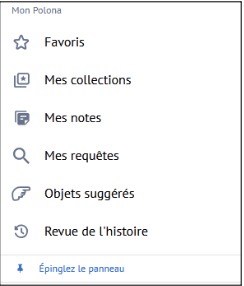
\includegraphics[width=0.4\textwidth]{./images/compte_personnel/IMG_5982.jpeg}
\end{center}

\textbf{Bodleian Library, bibliothèque numérique d’Oxford:}
\url{https://digital.bodleian.ox.ac.uk/login/?next=%2Fterms%2F}
 
L’utilisateur a la possibilité de se créer un compte afin de pouvoir enregistrer ses recherches et ses articles préférés. Il a plusieurs moyens pour se connecter via son compte Google, Oxford Single Sign-On ou avec un email et un mot de passe.

\begin{center}
	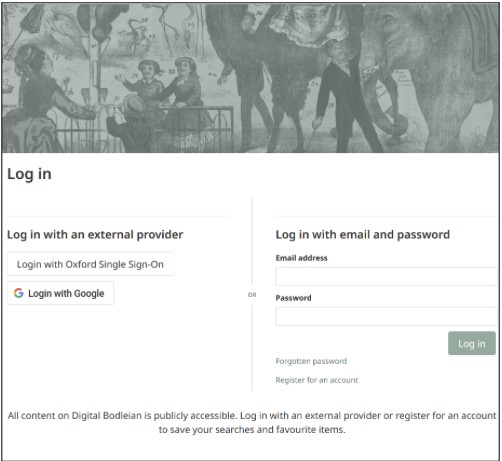
\includegraphics[width=0.5\textwidth]{./images/compte_personnel/IMG_5983.jpeg}
\end{center}

\textbf{Cariatide, bibliothèque numérique de l’INHA:}
\url{https://bibliotheque-numerique.inha.fr/mon-espace-personnel}

Dans Cariatide, la création d’un compte personnel permet à l’utilisateur d’enregistrer ses recherches, de configurer des notifications par mail, de sauvegarder, trier et partager les documents. Il y a deux moyens de connecter soit par son compte lecteur de l’INHA ou soit par celui de Cariatide.

\begin{center}
	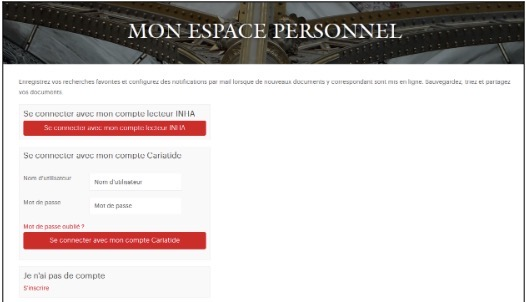
\includegraphics[width=0.5\textwidth]{./images/compte_personnel/IMG_5984.jpeg}
\end{center}

\textbf{Lucienne, bibliothèque numérique de l’ENS:}
\url{https://lucienne.ens.psl.eu/login?redirect_url=/s/lucienne/page/welcome}

Le compte personnel de Lucienne permet à l’usager de sélectionner les documents souhaités, d’écrire des notes personnelles, exporter la sélection.

\begin{center}
	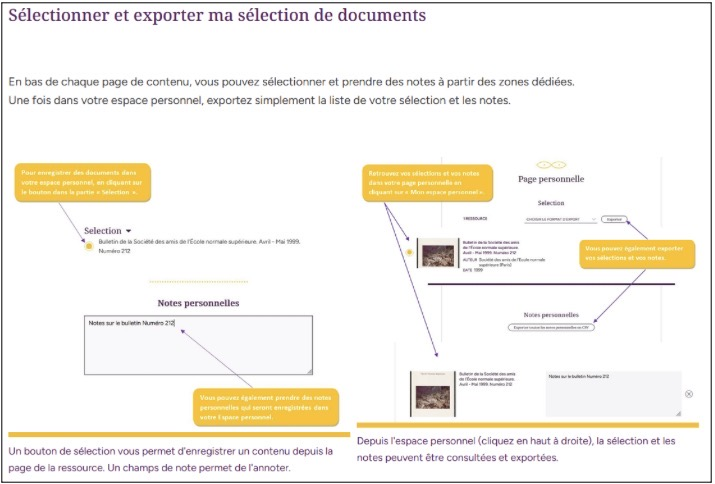
\includegraphics[width=0.5\textwidth]{./images/compte_personnel/IMG_5985.jpeg}
\end{center}

\textbf{Bibliothèque numérique de Sciences Po:}
\url{https://federation.sciences-po.fr/cas/login?service=https%3A%2F%2Fbibnum.sciencespo.fr%2Fcas%2Fvalidate}

La bibliothèque numérique de Sciences Po ayant la majorité de ses documents sous droits permet à ses utilisateurs leur consultation à partir d’une authentification. Cette authentification permet à l’étudiant, le chercheur de parcourir ses documents en fonction du statut du lecteur il n’a pas les mêmes options disponibles.

\begin{center}
	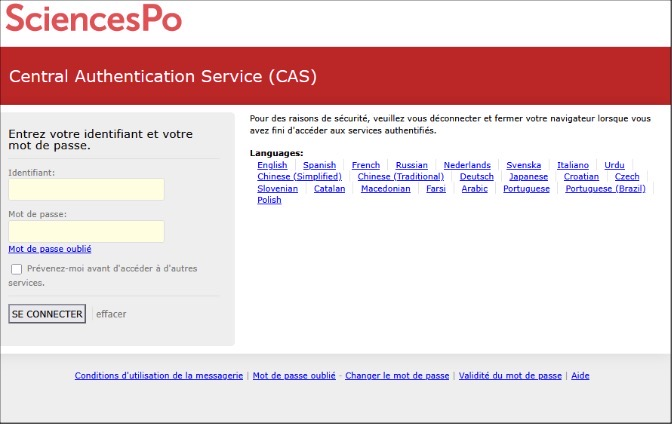
\includegraphics[width=0.5\textwidth]{./images/compte_personnel/IMG_5986.jpeg}
\end{center}

\subsubsection{Benchmark : la consultation des documents}
\textbf{Cambridge digital library:}

\url{https://cudl.lib.cam.ac.uk/view/PR-BASKERVILLE-BOX-00003/1}

Lorsque l’on consulte la visionneuse sur la bibliothèque numérique de l’université de Cambridge, celle-ci s’ouvre par défaut sur la visionneuse Universal Viewer permettant ainsi à des usagers moins expérimenté une prise en main rapide et une consultation du document simplifié.

\begin{center}
	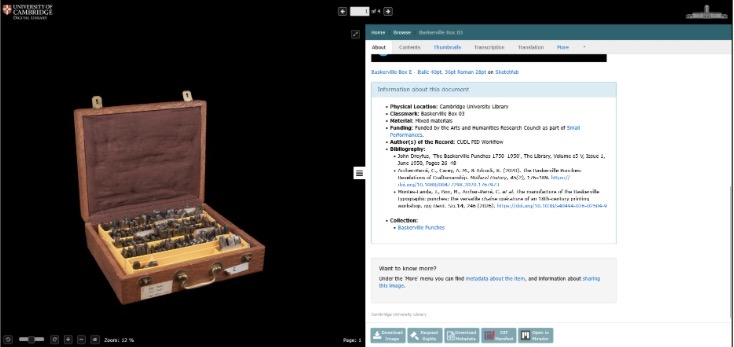
\includegraphics[width=0.5\textwidth]{./images/consultation_documents/IMG_5987.jpeg}
\end{center}

\textbf{Cambridge Digital Library:}

\url{https://cudl.lib.cam.ac.uk/mirador/PR-BASKERVILLE-BOX-00003/0}

Pour les usagers plus expérimentés ou aguerris, la CUDL a mis en place une autre visionneuse accessible depuis Universal Viewer en cliquant sur l’onglet de la visionneuse mirador permettant ainsi à ceux qui le souhaitent de la choisir pour travailler.

\begin{center}
	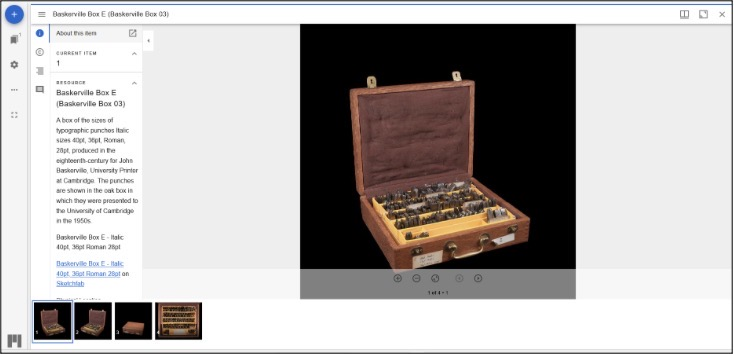
\includegraphics[width=0.5\textwidth]{./images/consultation_documents/IMG_5988.jpeg}
\end{center}

\textbf{NuBIS, bibliothèque numérique de la BIS:}

\url{https://nubis.bis-sorbonne.fr/viewer?manifest=https%3A%2F%2Fnubis.bis-sorbonne.fr%2Fiiif%2F2%2F924871%2Fmanifest}

La visionneuse Mirador possède divers avantages comme on peut le voir grâce aux nombreux outils de consultation des images (zoom, rotation, contraste).

Le bouton  est une autre fonctionnalité de Mirador permettant la réduction ou l’agrandissement de la fenêtre. 

\begin{center}
	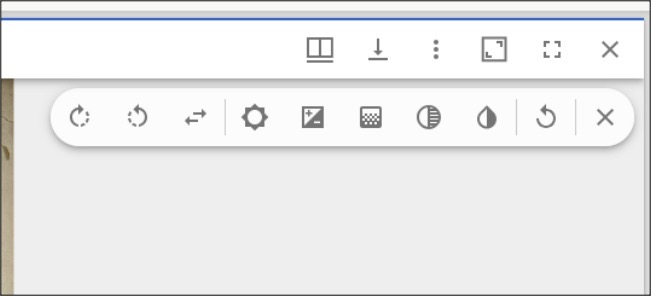
\includegraphics[width=0.5\textwidth]{./images/consultation_documents/IMG_5989.jpeg}
\end{center}

\textbf{NuBIS:}

\url{https://nubis.bis-sorbonne.fr/viewer?manifest=https%3A%2F%2Fnubis.bis-sorbonne.fr%2Fiiif%2F2%2F924871%2Fmanifest}

Mirador permet de choisir le mode de diffusion de l’image (simple, galerie), d’afficher les vignettes des différentes vues et de comparer des documents (cette fonctionnalité n’existe pas dans Universal Viewer).

\begin{center}
	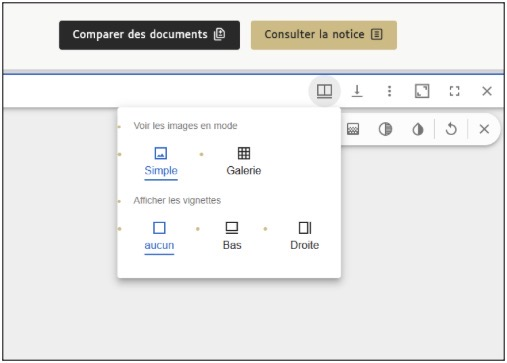
\includegraphics[width=0.5\textwidth]{./images/consultation_documents/IMG_5990.jpeg}
\end{center}

\subsubsection{Benchmark : exploitation des documents : options de téléchargements et formats disponibles}

\textbf{NuBIS, bibliothèque numérique de la BIS:}

\url{https://nubis.bis-sorbonne.fr/viewer?manifest=https%3A%2F%2Fnubis.bis-sorbonne.fr%2Fiiif%2F2%2F924871%2Fmanifest}

NuBIS propose plusieurs options de téléchargement d’images (JPEG), en changeant le nombre de pixels à chaque fois.

\begin{center}
	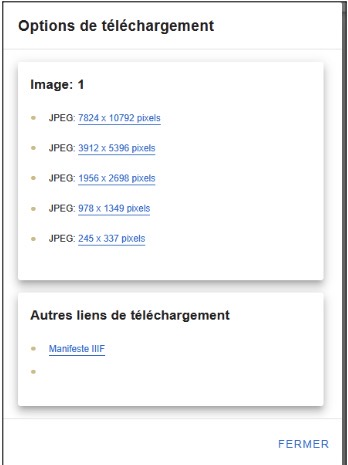
\includegraphics[width=0.4\textwidth]{./images/telechargements_et_formats/IMG_5991.jpeg}
\end{center}

\textbf{Gallica, bibliothèque numérique de la BNF:}

\url{https://gallica.bnf.fr/ark:/12148/bpt6k5473731s/f134.image.r=%22antoine%20felix%20de%20monti%22?rk=21459;2#}

La BNF permet lorsque l’on consulte un document de télécharger sous différents formats (PDF, JPEG, TXT) avec la possibilité de choisir entre le document entier ou une sélection.

\begin{center}
	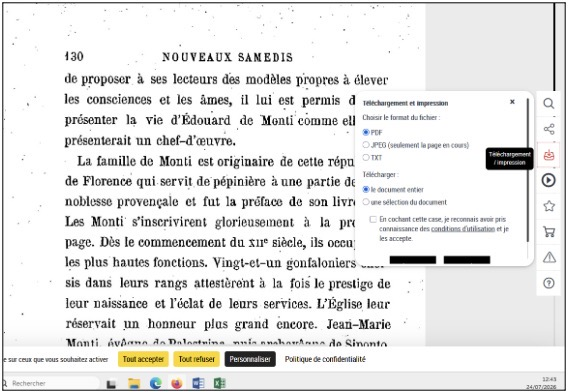
\includegraphics[width=0.5\textwidth]{./images/telechargements_et_formats/IMG_5992.jpeg}
\end{center}

\textbf{Digital Bodleian, bibliothèque numérique d’Oxford:}

\url{https://digital.bodleian.ox.ac.uk/objects/8bbd55ac-f9e2-4c02-9fcf-e36fd38a3645/} 

L’université d’Oxford donne également le choix pour le télécharger de plusieurs formats (PDF, JPEG), ainsi que la description de l’objet.

\begin{center}
	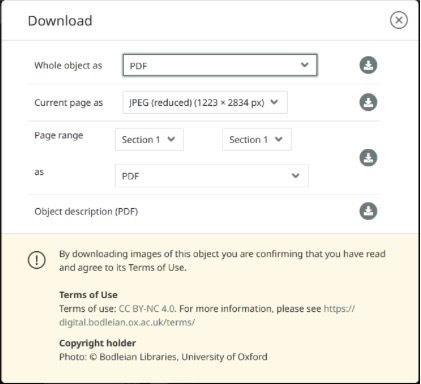
\includegraphics[width=0.5\textwidth]{./images/telechargements_et_formats/IMG_5993.jpeg}
\end{center}

\subsubsection{Benchmark : exploitation des documents : options de partage, d’annotation des documents}

\textbf{Gallica, bibliothèque numérique de la BNF:}

\url{https://gallica.bnf.fr/ark:/12148/bpt6k5473731s/f134.image.r=%22antoine%20felix%20de%20monti%22?rk=21459;2#}

La BnF offre plusieurs moyens de partager son document via mail, un lien, les réseaux sociaux.

\begin{center}
	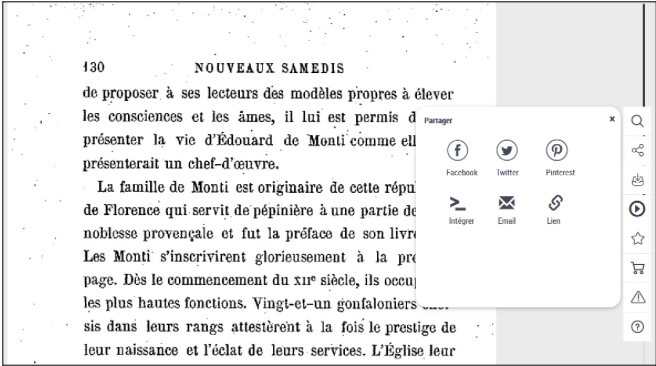
\includegraphics[width=0.5\textwidth]{./images/exploitation_documents/IMG_5994.jpeg}
\end{center}

\textbf{Lucienne, bibliothèque numérique de l’ENS:}

\url{https://lucienne.ens.psl.eu/s/lucienne/item/62457}

Lucienne permet la diffusion de ces documents libre de droit sur les réseaux sociaux (facebook, linkedin, whatsapp) ou par mail.

\begin{center}
	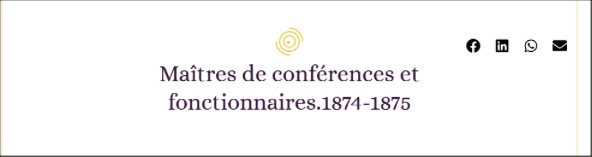
\includegraphics[width=0.5\textwidth]{./images/exploitation_documents/IMG_5995.jpeg}
\end{center}

\textbf{Cariatide, bibliothèque numérique de l’INHA:}

\url{https://bibliotheque-numerique.inha.fr/collection/item/59620-gazette-de-l-hotel-drouot-33-1913?offset=1}

Cariatide offre aussi la possibilité de partager ses documents par mail et par réseaux sociaux (facebook ou whatsapp).

\begin{center}
	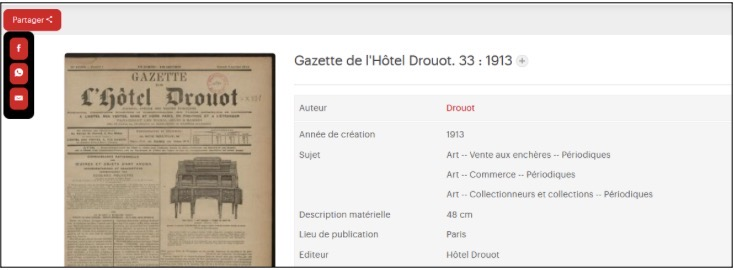
\includegraphics[width=0.5\textwidth]{./images/exploitation_documents/IMG_5996.jpeg}
\end{center}

\subsubsection{Benchmark : OCR, transcription}

\textbf{Cambridge Digital Library:}

\url{https://cudl.lib.cam.ac.uk/view/PR-07000-E-00374/10}

La CUDL offre la possibilité en fonction des documents d’avoir accès la transcription ou à la traduction du texte présent à l’image dans la visionneuse.

\begin{center}
	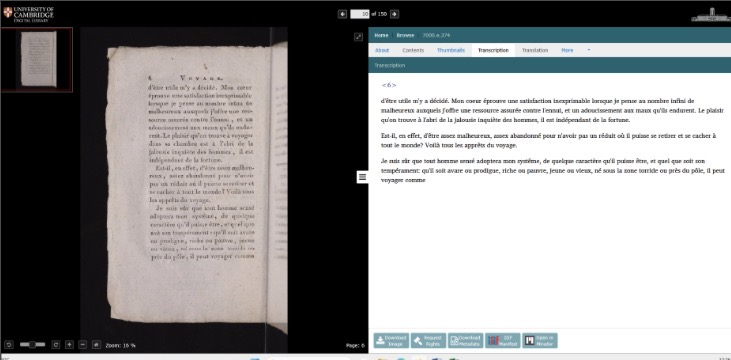
\includegraphics[width=0.6\textwidth]{./images/OCR_transcriptions/IMG_5997.jpeg}
\end{center}

\textbf{Gallica, bibliothèque numérique de la BNF:}

\url{https://gallica.bnf.fr/ark:/12148/bpt6k5473731s/f134.image.r=%22antoine%20felix%20de%20monti%22?rk=21459;2#}

La BnF permet à ses utilisateurs de faire une recherche OCR dans les documents qu’elle consulte afin de ne pas entrainer d’abus, elle a fixé un certain nombre de requête disponible, une fois le délai épuisé, l’utilisateur ne peut plus faire de recherche à l’intérieur devant attendre que le crédit se régénère. Cela n’a pas lieu quand on possède un compte personnel sur Gallica. Elle affiche également le nombre de résultats obtenus lorsque l’on a fait la recherche par mots dans tout le document.

\begin{center}
	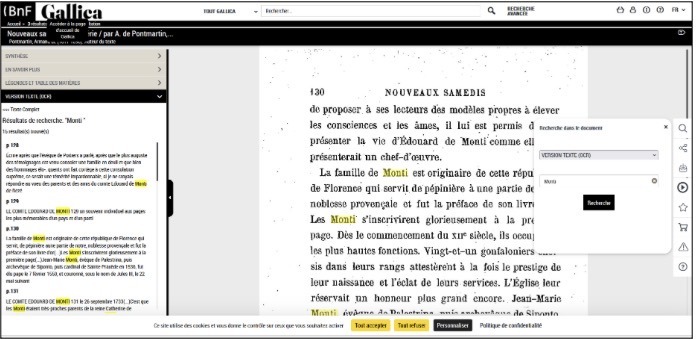
\includegraphics[width=0.6\textwidth]{./images/OCR_transcriptions/IMG_5998.jpeg}
\end{center}

\subsubsection{Benchmark : Droits d’accès et de réutilisation}

\textbf{Bibliothèque numérique de Sciences Po:}

\url{https://bibnum.sciencespo.fr/s/catalogue/access-request}

Pour les documents sous droits, comme l’université Sciences Po l’inscrit dans son document de droit d’accès des documents, les personnes extérieures à l’université doivent demander via ce formulaire l’autorisation de consulter un document de leur bibliothèque en indiquant le but dans lequel la recherche est effectuée.

\begin{center}
	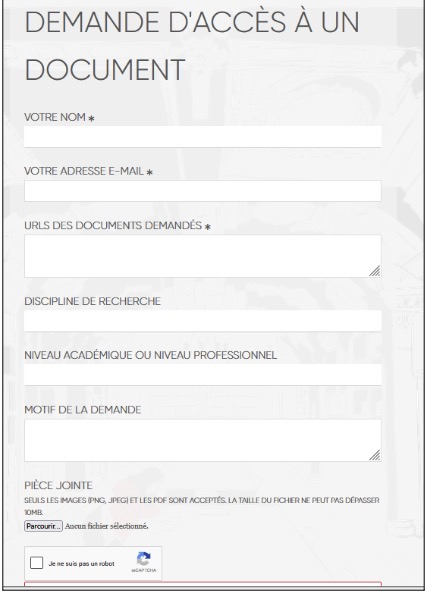
\includegraphics[width=0.5\textwidth]{./images/droit_acces/IMG_5999.jpeg}
\end{center}

\subsubsection{Proposition pour la bibliothèque numérique de Cujas}
\begin{itemize}
	\item \uline{Compte personnel:}
Il doit avoir deux modes de connexions: 
\begin{itemize}
	\item Une connexion utilisant l’identifiant et le mot de passe des lecteurs inscrits à Cujas
\item Une connexion via la création d’un compte lecteur pour les personnes non inscrites.
\end{itemize} 
Il doit être accessible depuis le menu de navigation sur la page d’accueil.
Il doit permettre aux lecteurs de mettre en favoris leurs documents, créer leurs propres collections, enregistrer des requêtes, configurer des notifications par mail, trier et partager les documents.
\item Consultation des documents: installer la visionneuse Mirador avec les fonctionnalités de comparaison des documents, de zoom, de rotation de l’image, de capture de  tout ou partie d’une image. 
\item Exploitation des documents : 
\begin{itemize}
	\item Proposer plusieurs formats de téléchargement (PDF, JPEG, TXT)
\item Permettre le téléchargement sélectif (une partie ou la totalité du document)
\item Ajouter sur la notice du document les options de partage des documents (facebook, whatsapp, email…).
\end{itemize}
Avec la visionneuse Mirador, il doit être possible de faire une recherche plein-texte à l’intérieur du document et de permettre aux personnes d’écrire des annotations.
\item Pour les documents sous droits, il faut créer un formulaire pour les personnes extérieures à l’université pouvant contenir les champs suivants : nom, mail, urls des documents demandés, niveau d’études, motifs de la demande.
\end{itemize}

\subsubsection{Eléments techniques}
\paragraph*{Module IIIF Server} 
\addcontentsline{toc}{paragraph}{Module IIIF Server}

Lien vers la documentation: \url{https://omeka.org/s/modules/IiifServer/}

Module permettant d’intégrer les spécifications IIIF pour permettre de traiter et de partager instantanément des images de toute taille et de tout média (pdf, audio, vidéo, 3D…) dans les formats souhaités. Il peut utiliser n’importe quel serveur d’image pour les afficher comme le module Image Server, Cantaloupe ou IIP Image. 

\paragraph*{Module Metadata browse}

Lien vers la documentation : \url{https://omeka.org/s/docs/user-manual/modules/metadatabrowse/}

Ce module permet de relier dynamiquement les documents entre eux de manière interne grâce à des critères communs (auteur, sujet, date).
Il permet de parcourir toutes les ressources qui partagent une valeur pour une propriété de métadonnées particulière. Il le fait en transformant les propriétés sélectionnées en un lien, ou en ajoutant un lien ci-dessous des prorpiétés qui se lit \enquote{voir tous les éléments avec cette valeur}.

\subsubsection{Réponse aux besoins identifiés par les personae}

Afin de valider la pertinence des choix fonctionnels proposés pour le compte personnel, la consultation et l’exploitation des documents, la synthèse ci-dessous illustre comment chaque fonctionnalité répond aux besoins prioritaires des personae :
\begin{itemize}
	\item \textbf{Besoin n°1 : Sauvegarder les requêtes et enregistrer les documents}
\begin{itemize}
	\item \uline{Personae concernés :} chercheur expert en histoire du droit, doctorante, étudiant et bibliothécaire.
\item \uline{Réponse :} Création d’un compte personnel pour le lecteur permettant de sauvegarder les requêtes, mettre en favoris les documents, paramétrer les notifications par mail, constituer ses collections, trier et partager les documents.
\end{itemize}
\item \textbf{Besoin n°2 : Comparer des documents, sélectionner une partie du texte}
\begin{itemize}
	\item \uline{Personae concernés :} chercheur expert en histoire du droit, doctorante, étudiant, bibliothécaire et l’amatrice éclairée.
\item \uline{Réponse :} Mise en place de la visionneuse Mirador permettant de comparer, d’annoter, de zoomer, d’obtenir le manifeste IIIF. Toutefois, la visionneuse ne permet pas d’ajouter toute l’arborescence de la table des matières des documents.
\end{itemize}
\item \textbf{Besoin n°3 : Télécharger une partie ou l’intégralité du document et recherché à l’intérieur}
\begin{itemize}
	\item \uline{Personae concernés :} chercheur expert en histoire du droit, doctorante, étudiant, bibliothécaire et responsable de la bibliothèque.
\item \uline{Réponse :} Mise à disposition de choisir entre télécharger uniquement la page en cours de consultation, ou tout le document sous différents formats (JPEG, PDF, TXT). Possible de faire une recherche par occurrence dans le document à partir de la visionneuse.
\end{itemize}
\item \textbf{Besoin n°4 : Accès aux documents sous droits}
\begin{itemize}
	\item \uline{Persona concerné :} Responsable de la bibliothèque numérique et bibliothécaire.
\item \uline{Réponse :} Création d’un formulaire pour les personnes extérieures à l’université devant justifier le motif de la consultation pour cet ouvrage et mettre en place des droits différenciés pour les personnes de l’université pour ce type de consultation.
\end{itemize}
\end{itemize}

\subsection{Valorisation, information et accompagnement des usagers}
\subsubsection{Les besoins identifiés}
\begin{itemize}
	\item Informations institutionnelles
\begin{itemize}
	\item Contact
\item Mentions légales
\item Politique de confidentialité (RGPD)
\item Conditions d’utilisation
\item Informations sur l’accessibilité (norme WCAG)
\end{itemize}
\item Accompagnement des usagers
\begin{itemize}
	\item FAQ
\item Tutoriels et guides de recherche
\end{itemize}
\item Valorisation 
\begin{itemize}
	\item Présentation des collections et des fonds
\item Exposition virtuelle
\item Articles 
\item Editions numériques (édition critique, transcription, annotation)
\item Galerie de personnalités 
\item Billets de blog 
\item Actualités
\end{itemize}
\end{itemize}

\subsubsection{Benchmark : Informations institutionnelles}

\paragraph*{Page « A propos »}
\addcontentsline{toc}{paragraph}{Page « A propos »}
Il s’agit généralement d’une présentation de la bibliothèque numérique, ses collections, ses acteurs. Des éléments concernant les conditions d’utilisation des documents et des éléments techniques peuvent y être joints. 

\textbf{Gallica, bibliothèque numérique de la BNF:}
\url{https://gallica.bnf.fr/accueil/fr/html/a-propos}

Dans la page « A propos » de Gallica sont exposés : 
\begin{itemize}
	\item L’histoire de la bibliothèque numérique
\item Une explication pour la distinguer de Gallica Intra muros (Gallica Intra-muros propose en consultation les documents « sous droits », à l’intérieur des murs de la BnF)
\item Une courte description des conditions d’utilisation et de reproduction des documents.
\end{itemize}

\begin{center}
	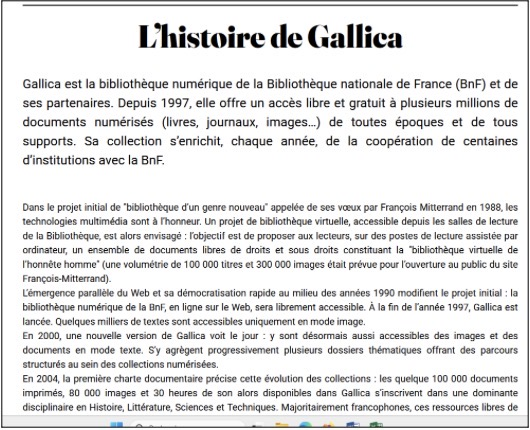
\includegraphics[width=0.5\textwidth]{./images/a_propos/IMG_6001.jpeg}
\end{center}

\textbf{Cambridge digital library:}
\url{https://cudl.lib.cam.ac.uk/about/}

L’ensemble des informations importantes sont rassemblées en un seul endroit et structurées en plusieurs parties : une introduction de la CUDL, l’actualité, la communauté, les contributeurs ainsi que les termes et conditions d’usages. 

\begin{center}
	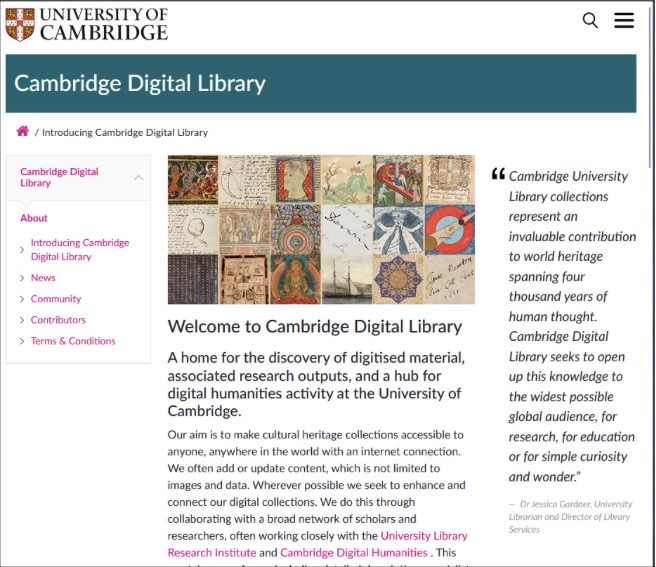
\includegraphics[width=0.5\textwidth]{./images/a_propos/IMG_6002.jpeg}
\end{center}

\textbf{Digital Bodleian, bibliothèque numérique d’Oxford:}
\url{https://digital.bodleian.ox.ac.uk/about/}

Sur cette page l’université d’Oxford présente : 
\begin{itemize}
	\item La nouvelle bibliothèque numérique et les collections que l’on va pouvoir y trouver 
\item Les services qu’elle a mis en place 
\item Des éléments de contact
\item Une brève présentation de l’équipe en charge de la bibliothèque numérique
\end{itemize}

\begin{center}
	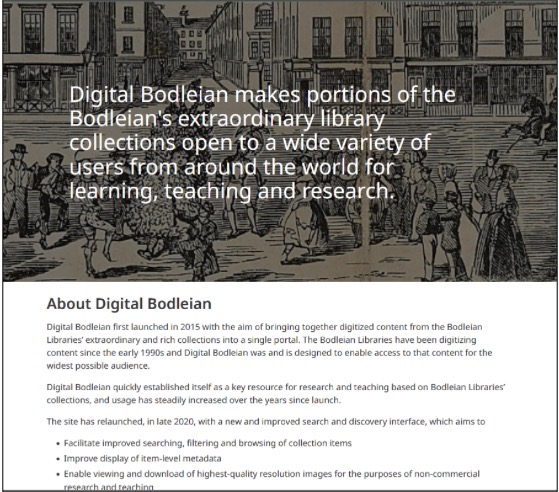
\includegraphics[width=0.5\textwidth]{./images/a_propos/IMG_6003.jpeg}
\end{center}

\textbf{Cariatide, bibliothèque numérique de l’INHA:}
\url{https://bibliotheque-numerique.inha.fr/}

La page d’accueil propose une courte présentation de la bibliothèque numérique et des fonds numérisés. 

\begin{center}
	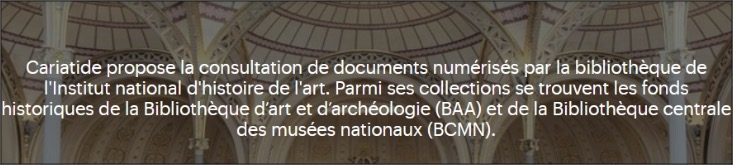
\includegraphics[width=0.5\textwidth]{./images/a_propos/IMG_6004.jpeg}
\end{center}

\textbf{Genovefa, Bibliothèque Sainte Geneviève:}
\url{https://genovefa.bsg.univ-paris3.fr/s/genovefa/page/accueil}  

La BSG présente sur sa page d’accueil brièvement les types de documents que les personnes vont trouver sur la bibliothèque numérique, les missions qui l’animent ainsi que la façon dont les fonds peuvent être explorés.

\begin{center}
	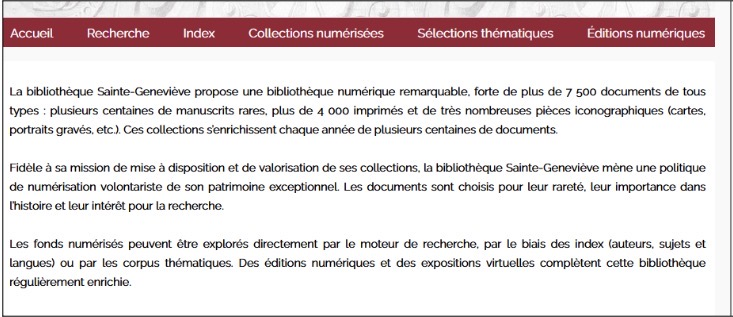
\includegraphics[width=0.5\textwidth]{./images/a_propos/IMG_6005.jpeg}
\end{center}

\textbf{NuBIS, bibliothèque numérique de la BIS:}
\url{https://nubis.bis-sorbonne.fr/a-propos/}

La BIS a fait le choix de centraliser les éléments présentant NuBIS dans la page « A propos » : 
\begin{itemize}
	\item Les corpus numérisés
\item Les aspects techniques concernant quatre points (la numérisation, l’OCR, les outils de diffusion et les métadonnées)
\item L’équipe de la BIS en charge du maintien et de l’alimentation de NuBIS
\end{itemize}

\begin{center}
	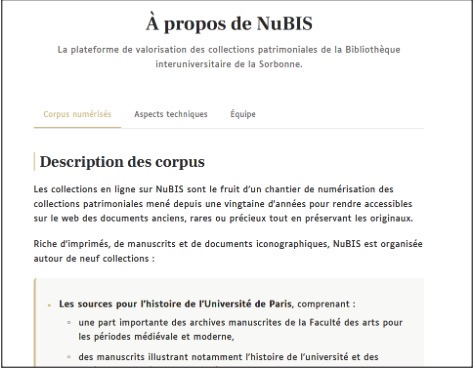
\includegraphics[width=0.5\textwidth]{./images/a_propos/IMG_6006.jpeg}
\end{center}

\paragraph*{Mentions légales} 

Les mentions légales, par définition obligatoires, comprennent la dénomination sociale et ses coordonnées, les mentions relatives à la propriété intellectuelle, les mentions relatives à l’hébergement du site, le nom du directeur de publication. Les bibliothèques numériques présentent ces informations sous forme plus ou moins développée, parfois jointes avec les informations relatives au RGPD et aux cookies. 

\textbf{Bibliothèque numérique de Sciences Po:}
\url{https://bibnum.sciencespo.fr/s/catalogue/page/mentions-legales}

La bibliothèque de Sciences Po propose sur la même page : 
\begin{itemize}
	\item Le propriétaire de la bibliothèque et son hébergeur2
\item Des éléments de responsabilité
\item Des éléments concernant la gestion des données personnelles
\item Des liens hypertextes pour aller vers d’autres sites web.
\end{itemize}

\begin{center}
	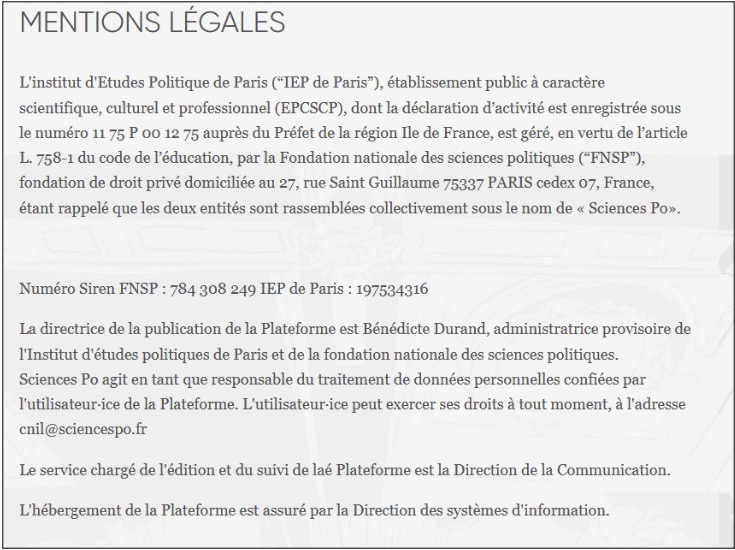
\includegraphics[width=0.5\textwidth]{./images/mentions_legales/IMG_6007.jpeg}
\end{center}

\textbf{Gallica, bibliothèque numérique de la BNF:}
\url{https://gallica.bnf.fr/accueil/fr/html/mentions-legales}

La BnF fait une brève présentation des mentions légales allant à l’essentiel en mentionnant l’éditeur du site et le directeur de publication.

\begin{center}
	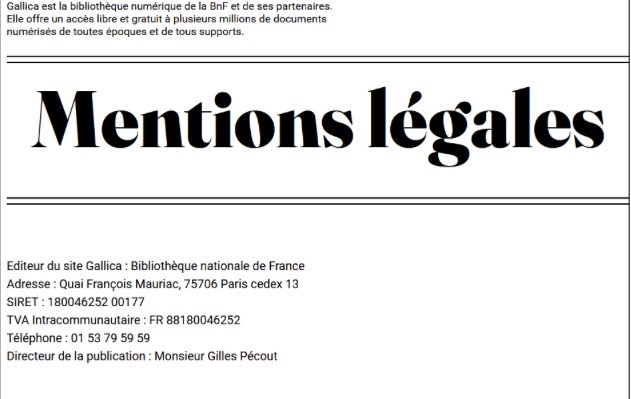
\includegraphics[width=0.5\textwidth]{./images/mentions_legales/IMG_6008.jpeg}
\end{center}

\textbf{Cariatide, bibliothèque numérique de l’INHA:}
\url{https://bibliotheque-numerique.inha.fr/mentions-legales}

L’INHA présente : 
\begin{itemize}
	\item Le directeur de la publication
\item L’éditeur
\item Les responsables de la conception et de la réalisation
\item L’hébergeur
\end{itemize}
Elle donne enfin des éléments de responsabilité des contenus, signale les liens sortant et donne des éléments de propriété intellectuelle. 

\begin{center}
	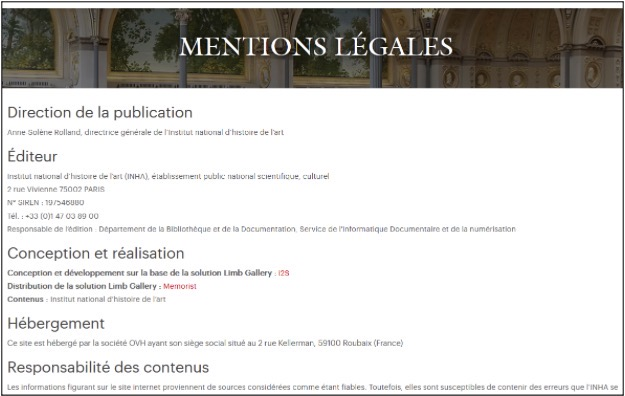
\includegraphics[width=0.5\textwidth]{./images/mentions_legales/IMG_6009.jpeg}
\end{center}

\textbf{NuBIS, bibliothèque numérique de la BIS:}
\url{https://nubis.bis-sorbonne.fr/mentions-legales/}

La BIS renseigne au même endroit les informations obligatoires demandées par le gouvernement et des éléments concernant le traitement des données personnelles (non collecte, usage de traceurs et de cookies de mesure d’audience anonymisés).

\begin{center}
	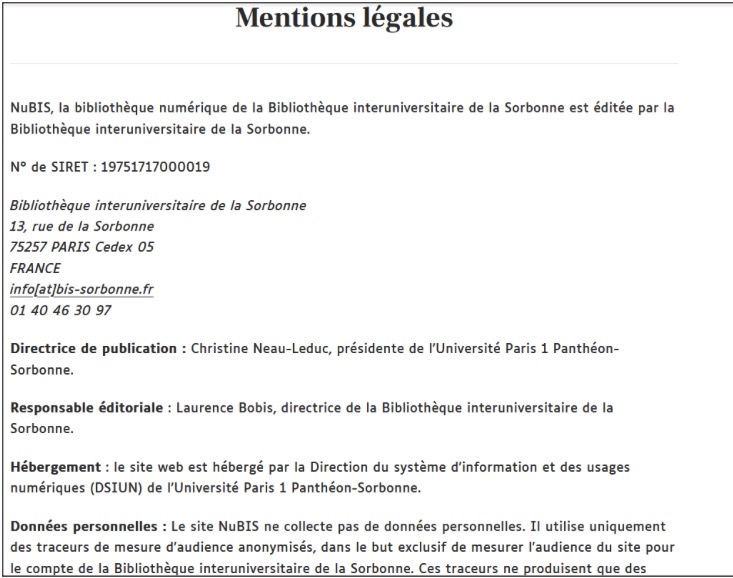
\includegraphics[width=0.5\textwidth]{./images/mentions_legales/IMG_6010.jpeg}
\end{center}

\textbf{Lucienne, bibliothèque numérique de l’ENS:}
\url{https://lucienne.ens.psl.eu/s/lucienne/page/mentions-legales}

L’ENS a fait le choix de rassembler sur une même page les mentions légales, les crédits ainsi que les conditions d’utilisation du site et de reproduction des images.

\begin{center}
	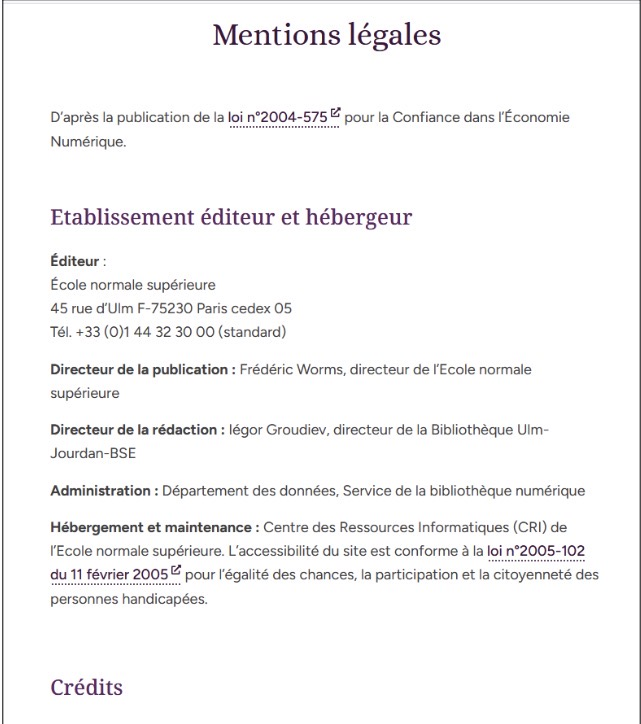
\includegraphics[width=0.5\textwidth]{./images/mentions_legales/IMG_6011.jpeg}
\end{center}

\paragraph*{Politique de confidentialité (RGPD)}

Cette mention obligatoire est généralement accessible depuis le pied de page. Elles sont parfois jointes aux mentions légales. 

\textbf{Digital Bodleian, bibliothèque numérique d’Oxford:}
\url{https://glam.web.ox.ac.uk/privacy-policy-digital-bodleian-website}

Un lien en pied de page renvoie à une page du site web de l’université concernant la bibliothèque numérique, mentionnant des éléments sur les utilisateurs des données personnelles assortis d’une définition précise de celles-ci, le type de données collectées et l’usage qui en est fait, leur lieu de stockage, leur durée de conservation, les droits des utilisateurs et des éléments concernant les cookies.

\begin{center}
	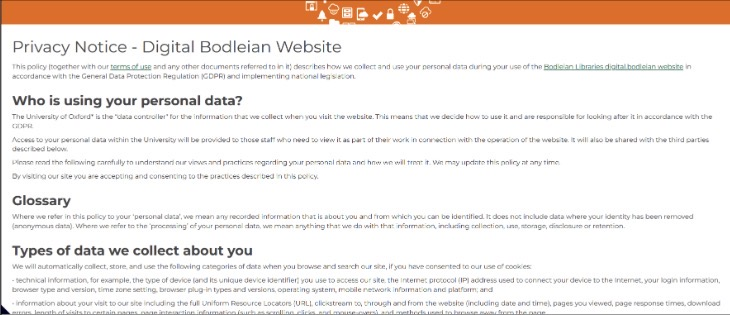
\includegraphics[width=0.5\textwidth]{./images/RGPD/IMG_6012.jpeg}
\end{center}

\textbf{Polona, bibliothèque numérique de la bibliothèque nationale de Pologne:} \url{https://polona.pl/static/polona/da364945-2bd1-4f6f-bb56-23846128b0dc}

Un lien en pied de page du site donne des explications sur la gestion des données personnelles (sécurité, mécanisme des cookies, collecte, usage).

\begin{center}
	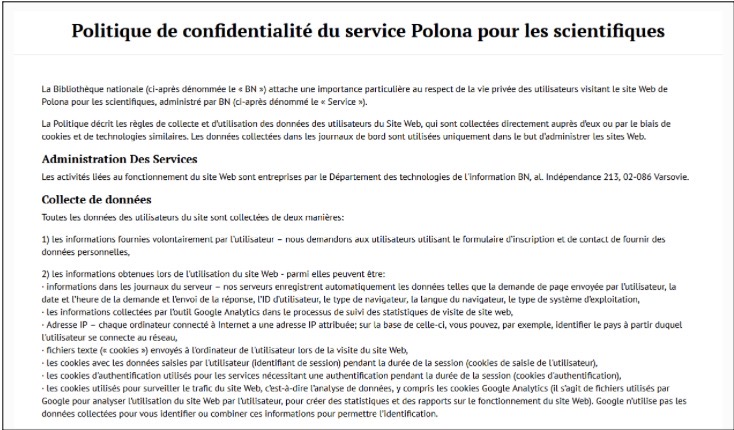
\includegraphics[width=0.5\textwidth]{./images/RGPD/IMG_6013.jpeg}
\end{center}

\textbf{Lucienne, bibliothèque numérique de l’ENS:}
\url{https://lucienne.ens.psl.eu/s/lucienne/page/politique-de-confidentialite}

Un lien en pied de page mène à une page \enquote{Politique de confidentialité} divisée en quatre grandes thématiques : généralités applicables aux traitements mis en œuvre, informations tenant à la collecte et au traitement sur le site internet des bibliothèques de l’ENS-PSL, du catalogue et de la bibliothèque numérique et pour finir la gestion des cookies et traceurs, assorti d’un contact pour joindre la déléguée à la protection des données personnelles.

\begin{center}
	
\includegraphics[width=0.5\textwidth]{./images/RGPD/IMG_6014.jpeg}
\end{center}

\paragraph*{Conditions d’utilisation}

Les conditions d’utilisation des documents numérisés sont toujours abordées de façon précise dans les bibliothèques numériques analysées. Des licences Etalab ou Creative Commons peuvent être appliquées aux documents. Ces informations sont parfois complétées de liens vers une documentation complémentaire. Des outils de réutilisation et de partage peuvent être mentionnés. Les conditions d’utilisation peuvent enfin être présentées avec la politique de confidentialité (RGPD). 

\textbf{Digital Bodleian, bibliothèque numérique d’Oxford:}
\url{https://digital.bodleian.ox.ac.uk/terms/}

Les conditions d’utilisation sont abordées à travers une table des matières cliquable qui décrit les conditions d’utilisation, les usages autorisés et interdits, la stabilité des accès aux informations, l’application du droit d’auteur, la responsabilité de l’institution. 

\begin{center}
	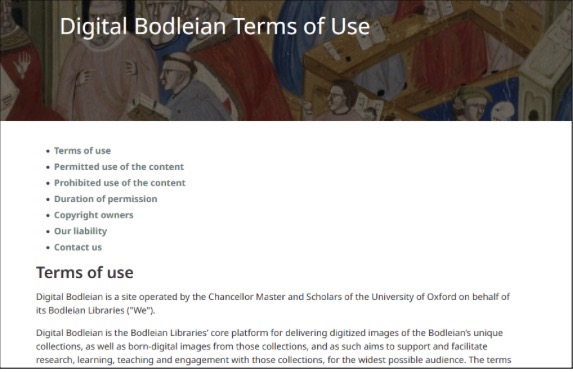
\includegraphics[width=0.5\textwidth]{./images/conditions_utilisation/IMG_6015.jpeg}
\end{center}

\textbf{Polona, bibliothèque numérique de la bibliothèque nationale de Pologne:}
\url{https://polona.pl/static/polona/polona-regulamin}

La bibliothèque nationale de Pologne propose un règlement très précis concernant l’usage de la bibliothèque numérique. Le site précise la procédure d’utilisation de la bibliothèque, ce que les usagers ont le droit de faire, mais aussi des mesures que le personnel de la BCP a le droit de prendre en fonction de situation prédéfinies dans le règlement.

\begin{center}
	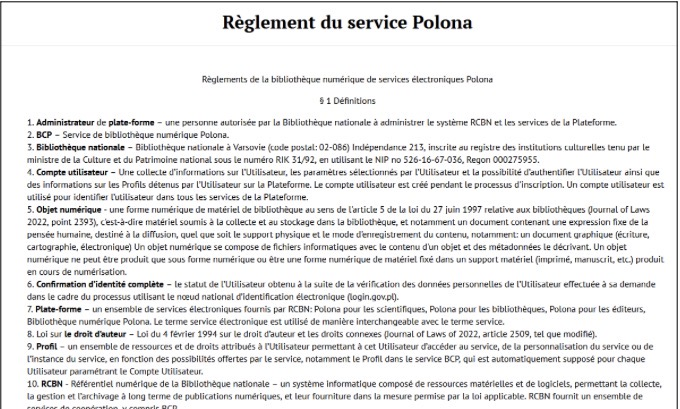
\includegraphics[width=0.5\textwidth]{./images/conditions_utilisation/IMG_6016.jpeg}
\end{center}

\textbf{Gallica, bibliothèque numérique de la BNF:}
\url{https://gallica.bnf.fr/accueil/fr/html/conditions-dutilisation-de-gallica}

La BNF propose une page accessible depuis le pied de page de Gallica. Celle-ci les conditions et les modalités d’utilisation du site, les conditions d’accès au site ainsi que l’engagement et les responsabilités de l’internaute. La BNF explique brièvement les raisons qui font qu’elle collecte les données personnelles des usagers.

\begin{center}
	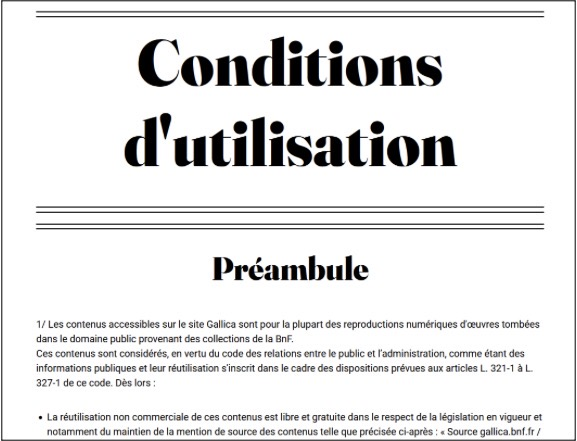
\includegraphics[width=0.5\textwidth]{./images/conditions_utilisation/IMG_6017.jpeg}
\end{center}

\textbf{Cariatide, bibliothèque numérique de l’INHA:}
\url{https://bibliotheque-numerique.inha.fr/conditions-utilisation}

L’INHA explique que tous ses documents numérisés se trouvent sous la licence Ouverte / Open Licence, Etalab. Elle présente brièvement les outils mis à disposition pour réutiliser les notices, les partager, ainsi que les outils mis à disposition dans la visionneuse.

\begin{center}
	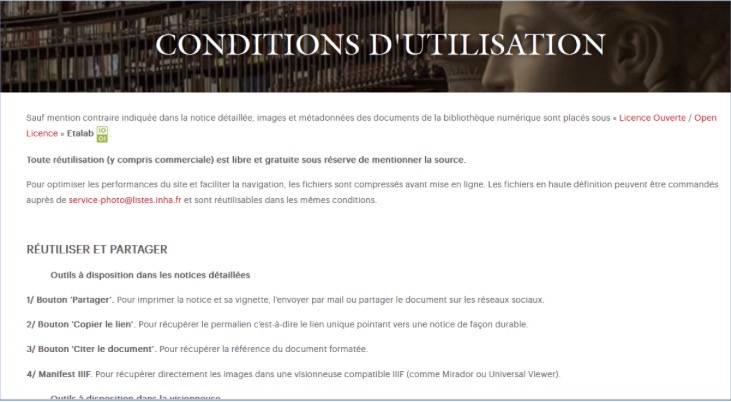
\includegraphics[width=0.5\textwidth]{./images/conditions_utilisation/IMG_6018.jpeg}
\end{center}

\textbf{NuBIS, bibliothèque numérique de la BIS:}
\url{https://nubis.bis-sorbonne.fr/conditions-d-utilisation/}

La BIS distingue clairement les droits pour les documents librement réutilisables et les droits pour les documents sous droits. Elle indique que les documents publics se trouvent sous la licence Etalab, et que les documents sous droits se trouvent sous la licence Creative Commons CC BY-NC-ND version 4.0 (droit à la diffusion, mais pas d’utilisation commerciale). Elle donne également accès à des ressources complémentaires afin de compléter l’information des usagers sur la réutilisation des images (Guide de l’INHA). 

\begin{center}
	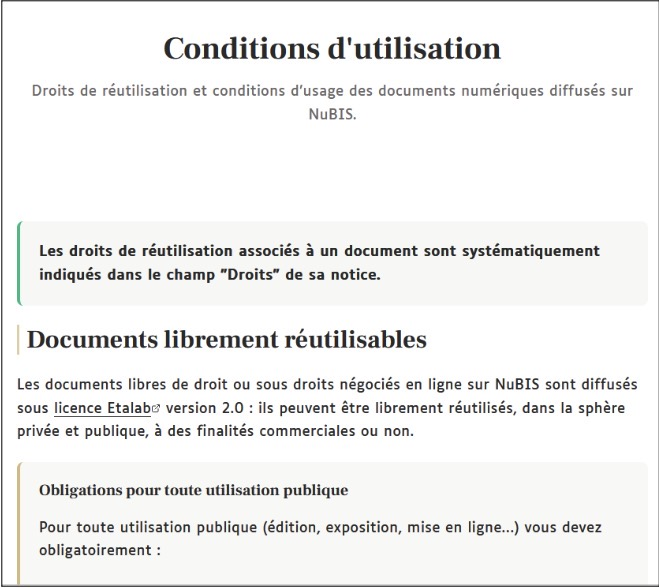
\includegraphics[width=0.5\textwidth]{./images/conditions_utilisation/IMG_6019.jpeg}
\end{center}

\paragraph*{Accessibilité (norme WCAG)}

Les bibliothèques numériques proposent généralement une Déclaration d’accessibilité en pied de page qui explicitent clairement l’état d’accessibilité des sites, souvent partiel. De rares bibliothèques numériques proposent la possibilité de paramétrer l’affichage à des fins d’accessibilité. 

\textbf{Digital Bodleian, bibliothèque numérique d’Oxford:}
\url{https://visit.bodleian.ox.ac.uk/website-accessibility}

La Digital Bodleian Library propose depuis le pied de page un lien vers une déclaration d’accessibilité. Elle y signale un site partiellement accessible et en explique les raisons. L’université explique comment elle teste l’accessibilité de ses sites Web et reste à attentive aux retours des usagers qui leur signalent des problèmes.

\begin{center}
	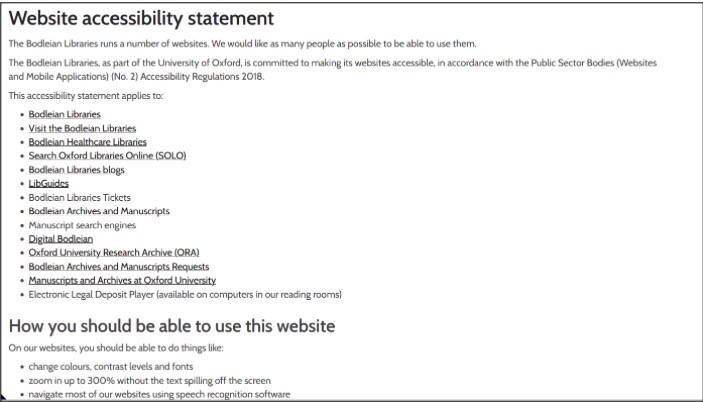
\includegraphics[width=0.5\textwidth]{./images/WCAG/IMG_6020.jpeg}
\end{center}

\textbf{Cariatide, bibliothèque numérique de l’INHA:}
\url{https://bibliotheque-numerique.inha.fr/accessibilite}

La déclaration d’accessibilité est accessible depuis le pied de page. Elle évoque de façon transparente l’état de conformité du site, les résultats des tests menés et liste les contenus non accessibles. Une particularité propre à l’INHA extrêmement utile est de mettre à disposition sur toutes ses pages des options d’accessibilité (police dyslexie, contrastes renforcés, augmenter le texte) permettant à l’utilisateur de cocher celle dont il a besoin.

\begin{center}
	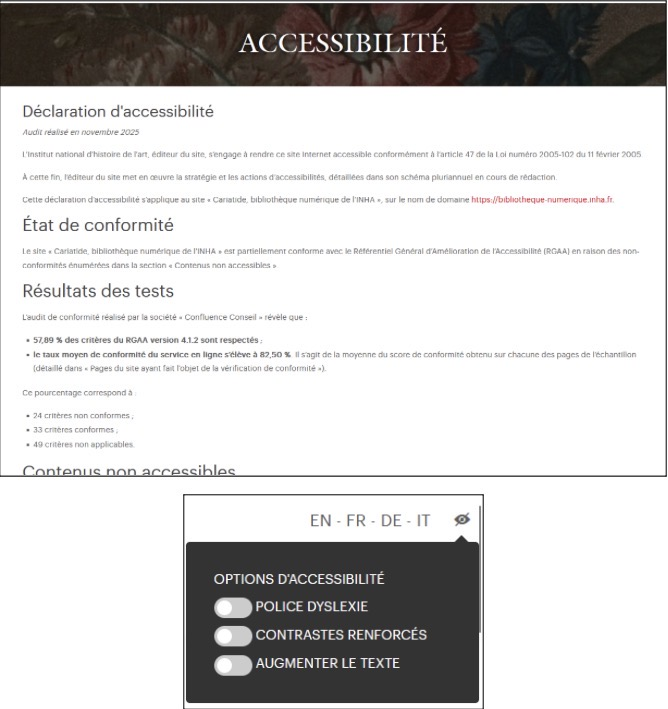
\includegraphics[width=0.5\textwidth]{./images/WCAG/IMG_6021.jpeg}
\end{center}

\textbf{Lucienne, bibliothèque numérique de l’ENS:}
\url{https://lucienne.ens.psl.eu/s/lucienne/page/accessibilite}

L’ENS propose depuis le pied e page une déclaration d’accessibilité transparent. Elle y indique pourquoi le site est partiellement conforme. Un audit a été réalisé par l’entreprise de studio web indépendant Kaeness, qui liste précisément toutes les pages ayant fait l’objet de la vérification de conformité. 

\begin{center}
	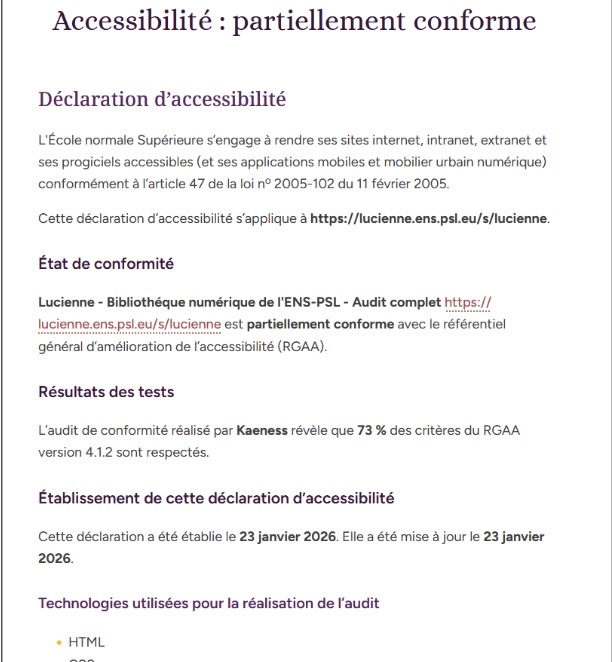
\includegraphics[width=0.5\textwidth]{./images/WCAG/IMG_6022.jpeg}
\end{center}

\paragraph*{Contact}

Généralement accessible depuis le pied de page, parfois en rubrique d’aide, le contact peut prendre la forme d’un mail cliquable ou d’un formulaire de contact. D’autres adresses peuvent être proposées afin d’orienter correctement les différentes demandes. 

\textbf{Gallica, bibliothèque numérique de la BNF:}
\url{https://gallica.bnf.fr/accueil/fr/html/contact}

En pied de page (footer), Gallica a mis un lien vers la page contact où elle donne l’adresse à laquelle les utilisateurs peuvent contacter la bibliothèque concernant une demande, signaler un problème, faire part d’une suggestion. Un lien vers un service de réponse à des questions bibliographiques est proposé depuis le même endroit invitant les lecteurs à orienter correctement leurs messages. 

\begin{center}
	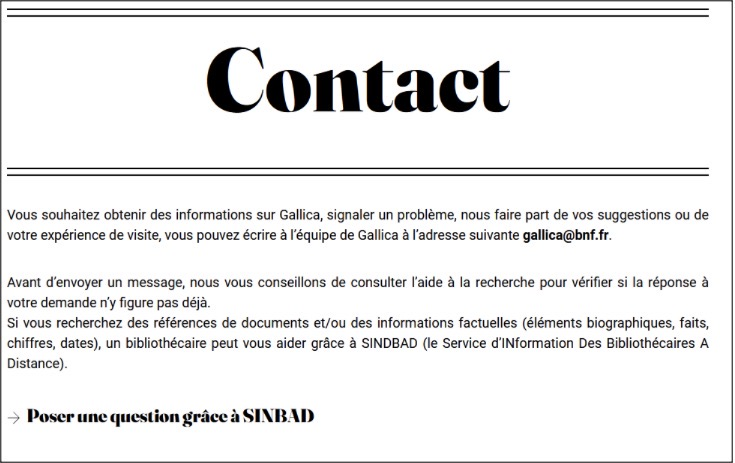
\includegraphics[width=0.5\textwidth]{./images/contact/IMG_6023.jpeg}
\end{center}

\textbf{Cariatide, bibliothèque numérique de l’INHA:}
\url{https://bibliotheque-numerique.inha.fr/contact}

Un formulaire de contact est accessible depuis le pied de page ou depuis l’onglet à propos. Il concerne uniquement les demandes à propos de la bibliothèque numérique ou des fonds numérisés. Pour toutes autres renseignements ou demandes concernant la réutilisation des images, Cariatide a transmis deux adresses mails séparés pour répondre à chaque cas.

\begin{center}
	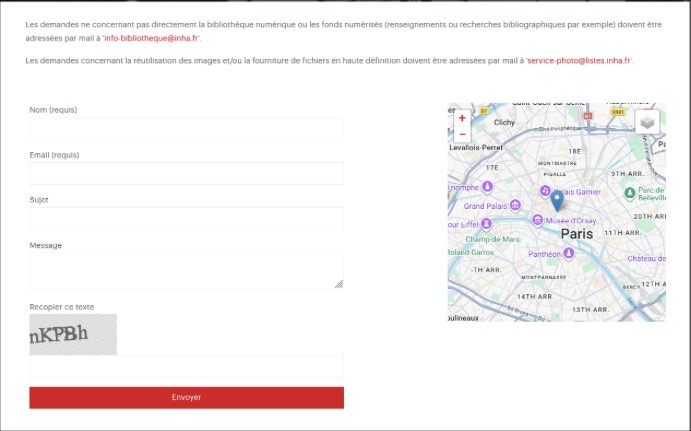
\includegraphics[width=0.5\textwidth]{./images/contact/IMG_6024.jpeg}
\end{center}

\textbf{NuBIS, bibliothèque numérique de la BIS:}
\url{https://nubis.bis-sorbonne.fr/aide/}

Une adresse mail est indiquée sur la page d’aide de NuBIS (accessible également depuis le pied de page) afin d’envoyer des remarques, questions, ou demandes. 

\begin{center}
	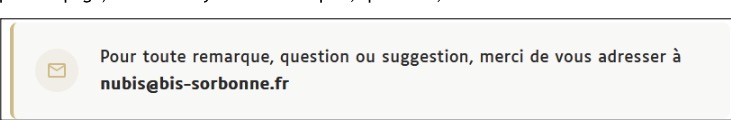
\includegraphics[width=0.5\textwidth]{./images/contact/IMG_6025.jpeg}
\end{center}

\textbf{Lucienne, bibliothèque numérique de l’ENS:}
\url{https://lucienne.ens.psl.eu/s/lucienne/page/contact}

Le lien de contact se trouve uniquement en pied de page et renvoie à un formulaire. Aucune adresse mail n’est indiquée. L’utilisateur doit obligatoirement cocher une case afin d’autoriser la bibliothèque à enregistrer le mail pour répondre au message. 

\begin{center}
	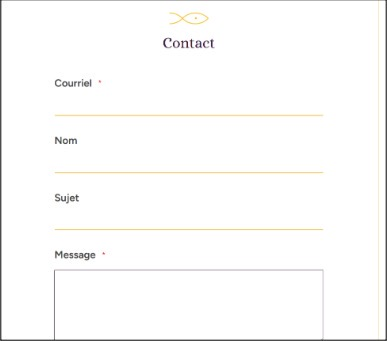
\includegraphics[width=0.5\textwidth]{./images/contact/IMG_6026.jpeg}
\end{center}

\subsubsection{Benchmark : Accompagnement des usagers}
\paragraph*{Tutoriels et guides de recherche}

Certaines bibliothèques numériques mettent à disposition des explications détaillées pour apprendre à chercher, consulter et exploiter les documents. Certaines proposent des modules d’aide technique en particulier concernant les API afin de mieux disséminer leurs données. 

\textbf{Polona, bibliothèque numérique de la bibliothèque nationale de Pologne:}
\url{https://polona.pl/static/POLONA/instrukcja-polona/konto-uzytkownika}

Un manuel d’utilisation est proposé aux utilisateurs souhaitant utiliser les collections numérisées par la BCP. Il est structuré en quatre thématiques (compte utilisateur, navigation sur le site, recherche, contact). 

\begin{center}
	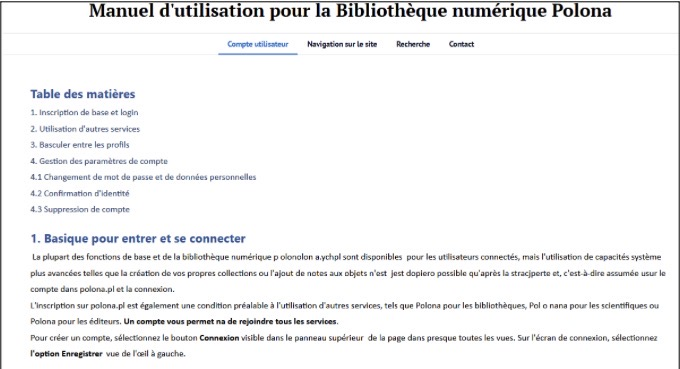
\includegraphics[width=0.5\textwidth]{./images/tutoriels/IMG_6027.jpeg}
\end{center}

\textbf{Gallica, bibliothèque numérique de la BNF:}
\url{https://gallica.bnf.fr/accueil/fr/html/aide-a-la-recherche}

Sa page d’aide à la recherche est une mine d’information permettant à l’usager de prendre en main Gallica. La BNF a fait le choix de varier les formes de contenus sur cette page et propose de courtes vidéos youtube sous la forme de sketchnote afin de présenter de façon ludique les tutoriels d’aide à la recherche. Des explications sont proposées à propos de la recherche de documents, de l’OCR et du mode texte, des formats de téléchargement et du partage des documents. 

\begin{center}
	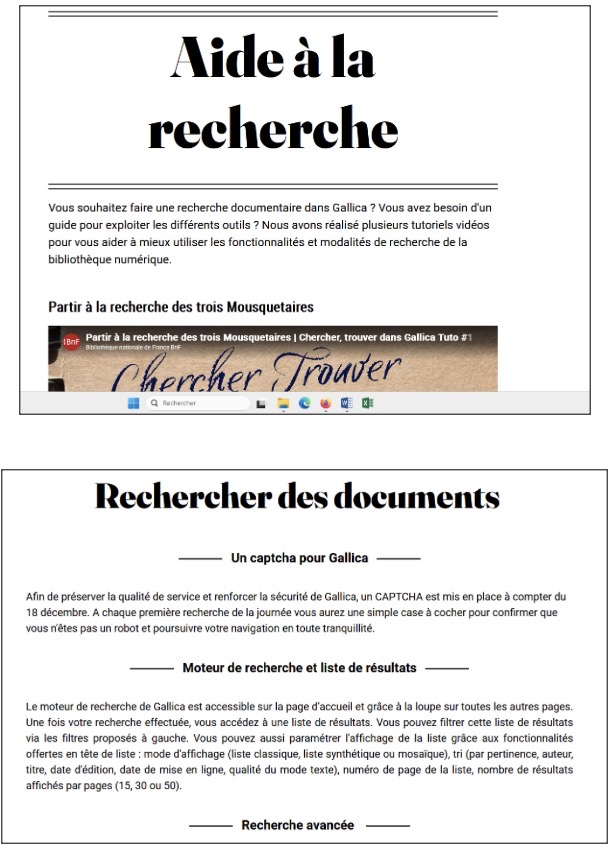
\includegraphics[width=0.5\textwidth]{./images/tutoriels/IMG_6028.jpeg}
\end{center}

\textbf{Digital Bodleian, bibliothèque numérique d’Oxford:}
\url{https://digital.bodleian.ox.ac.uk/help/}

L’université d’Oxford a créé un guide d’utilisation de la Digital Bodleian expliquant thématiques par thématiques comment prendre en main la bibliothèque. Par exemple, elle explique le fonctionnement de son outil de recherche (simple, avancée, facettes).

\begin{center}
	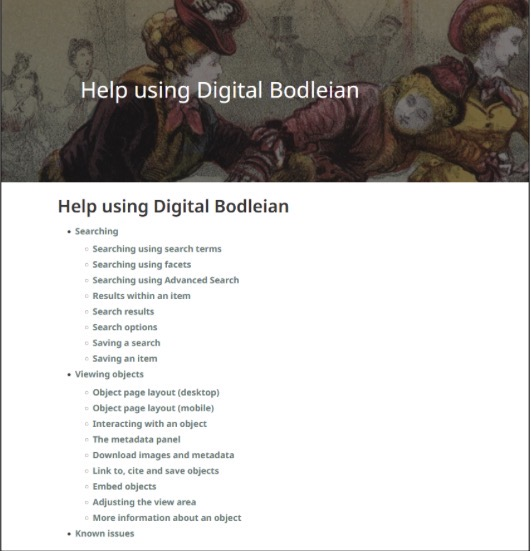
\includegraphics[width=0.5\textwidth]{./images/tutoriels/IMG_6029.jpeg}
\end{center}

\textbf{Documentation à propos des API:}
Digital Bodleian Library : \url{https://digital.bodleian.ox.ac.uk/developer/}

Dans son menu de navigation, elle propose également une documentation sur les API que la bibliothèque numérique utilise, en particulier l’API IIIF Documentation et l’API Documentation (Digitial Bodleian Search and Data).

\begin{center}
	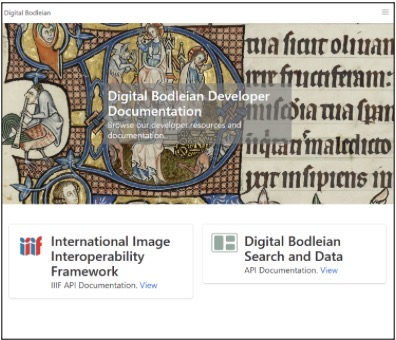
\includegraphics[width=0.5\textwidth]{./images/tutoriels/IMG_6030.jpeg}
\end{center}

\textbf{Cariatide, bibliothèque numérique de l’INHA:}
\url{https://bibliotheque-numerique.inha.fr/aide}

Sa page d’aide est accessible à partir de la rubrique \enquote{À propos}. Sur cette page, l’INHA explique comment découvrir ses collections, faire une recherche (simple, avancée), consulter un document. Elle détaille les outils présents dans la visionneuse.

\begin{center}
	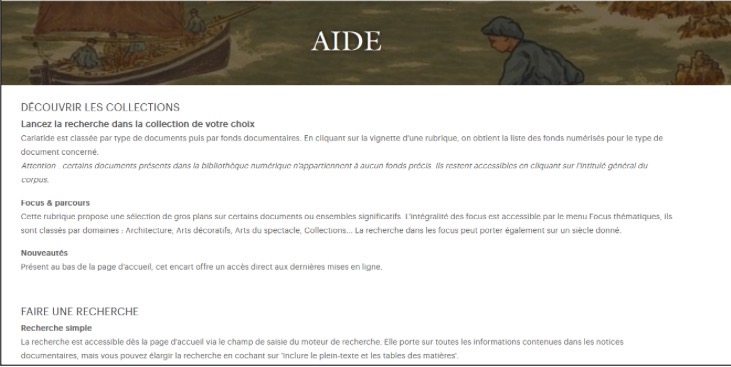
\includegraphics[width=0.5\textwidth]{./images/tutoriels/IMG_6031.jpeg}
\end{center}

\paragraph*{Les FAQ}

\textbf{Cambridge Digital Library:}
\url{https://cudl.lib.cam.ac.uk/help/#}

L’université de Cambridge a choisi de présenter l’aide à la prise en main de la bibliothèque sous la forme d’une foire aux questions (FAQ). C’est simple et rapide et permet de trouver directement l’information recherchée si la question a été traitée.

\begin{center}
	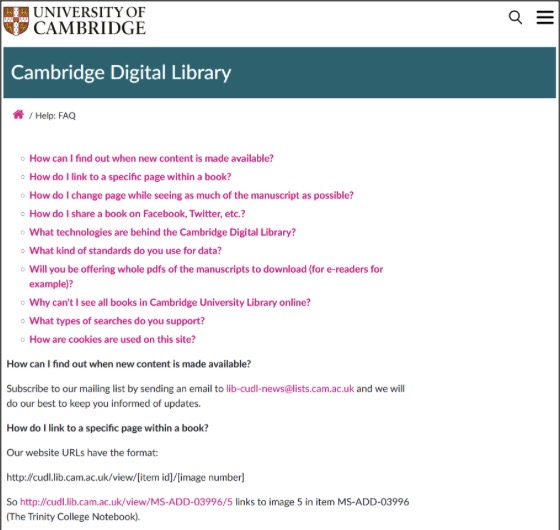
\includegraphics[width=0.5\textwidth]{./images/FAQ/IMG_6032.jpeg}
\end{center}

\textbf{Digital Bodleian, bibliothèque numérique d’Oxford:}
\url{https://digital.bodleian.ox.ac.uk/faq/#}

La FAQ centralise les réponses aux questions fréquemment posées concernant la bibliothèque numérique. Les questions les plus courantes sont traitées et les réponses immédiatement accessibles aux lecteurs. 

\begin{center}
	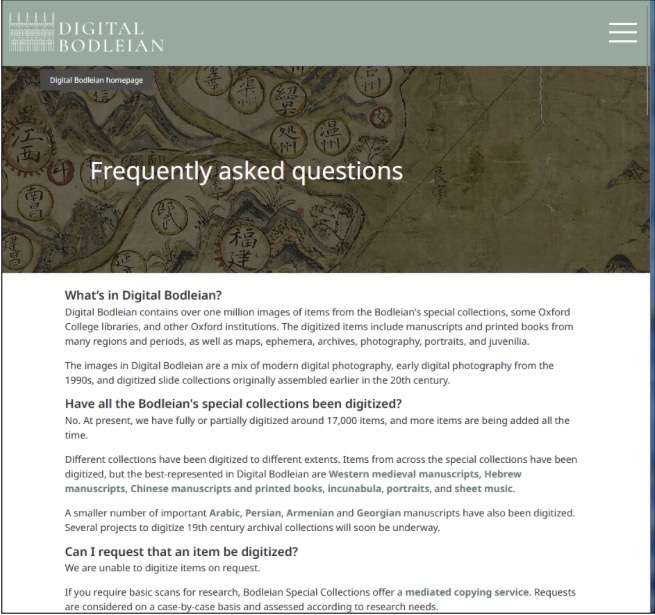
\includegraphics[width=0.5\textwidth]{./images/FAQ/IMG_6033.jpeg}
\end{center}

\textbf{NuBIS, bibliothèque numérique de la BIS:}
\url{https://nubis.bis-sorbonne.fr/aide/}

NuBIS a fait le choix de présenter sa FAQ sous la forme originale d’un menu déroulant : L’utilisateur ne déploie que la réponse de la question qui l’intéresse. La liste s’en trouve condensée et la recherche de la question souhaitée plus rapide. 

\begin{center}
	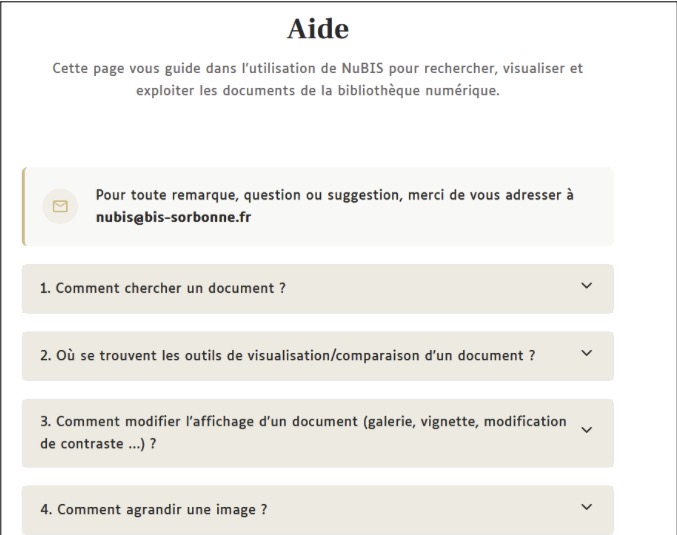
\includegraphics[width=0.5\textwidth]{./images/FAQ/IMG_6034.jpeg}
\end{center}

\subsubsection{Benchmark : Valorisation} 
La valorisation des collections numérisées prend de multiple formes en fonction des types de documents mis en ligne et de l’ampleur de la collection numérique. 
Les documents sont généralement organisés en collections. Ces collections peuvent être des regroupements thématiques, des regroupements de documents autour d’une personnalité, ou des fonds documentaires présents dans les collections physiques. La distinction entre regroupement de documents et fonds documentaires n’est pas toujours inscrite dans la structure de la bibliothèque numérique et ces éléments sont souvent mêlés. 
L’éditorialisation de ces collections peut prendre plusieurs formes : description, historique, sélection, article, exposition virtuelle, galeries de personnalités, fiches biographiques… Certaines bibliothèques numériques présentent des projets d’édition numérique réalisées avec leurs collections. 
Des actualités ou des billets de blogs permettent de tenir informés les lecteurs des nouveaux développements. 

\paragraph*{Présentation et éditorialisation des collections et des fonds}

\textbf{NuBIS, bibliothèque numérique de la BIS:}
Exemple : collection Histoire de la BIS : \url{https://nubis.bis-sorbonne.fr/collections/10366}

Une courte description de la collection indique au lecteur son contenu et le contexte de création de celle-ci. On distingue clairement les quatre sous-collection qui la structurent, chacune accompagnée d’une description qui lui est propre. 

\begin{center}
	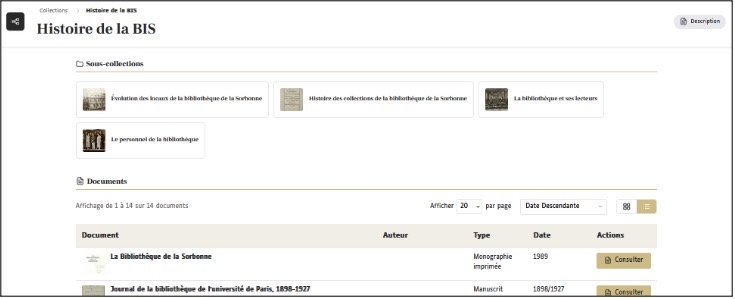
\includegraphics[width=0.5\textwidth]{./images/presentation_editorialisation/IMG_6035.jpeg}
\end{center}

\paragraph*{Contenu de la description :}

\textbf{Cambridge Digital Library:}
\url{https://cudl.lib.cam.ac.uk/collections/batesonarchive/1}

L’université de Cambridge a fait le choix d’éditorialiser la présentation de ses collections. La structure de la collection est présentée dans le texte de présentation. Les collections peuvent contenir des documents numérisés d’une personne ou sur une thématique. 

\begin{center}
	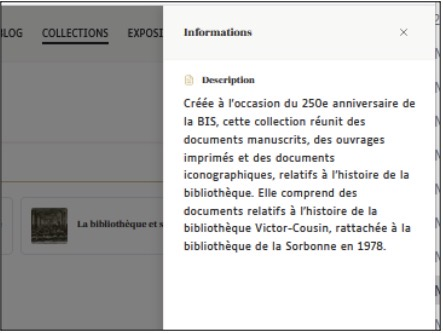
\includegraphics[width=0.5\textwidth]{./images/presentation_editorialisation/IMG_6036.jpeg}
\end{center}

\textbf{Digital Bodleian, bibliothèque numérique d’Oxford:}
\url{https://digital.bodleian.ox.ac.uk/collections/incunabula/}

Pour chacune de ses collections, l’université d’Oxford présente brièvement chaque collection et quels types d’ouvrages elle regroupe. Elle précise parfois comment les documents ont été acquis, comme pour ceux qui constituent sa collection d’incunables.

\begin{center}
	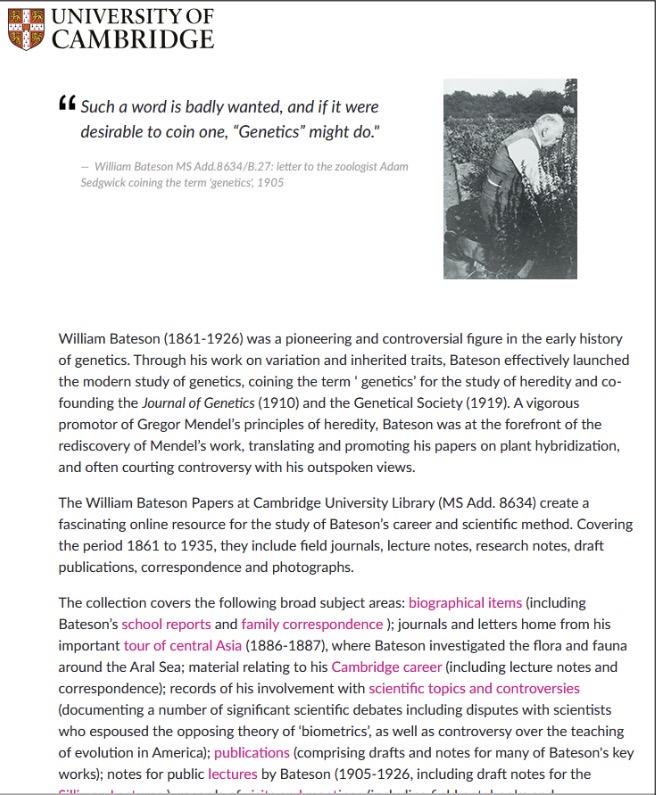
\includegraphics[width=0.5\textwidth]{./images/presentation_editorialisation/IMG_6037.jpeg}
\end{center}

\textbf{Genovefa, Bibliothèque Sainte Geneviève:}
\url{https://genovefa.bsg.univ-paris3.fr/s/genovefa/page/cartes_et_plans}

La BSG présentent chacune de ses collections en indiquant la provenance des documents qui la composent et des informations sur la publication. S’il s’agit d’un fonds personnel, la personne ayant possédé le fonds est brièvement présentée. Des liens vers d’autres fonds ou documents peuvent être tissés depuis la présentation, comme c’est le cas depuis la présentation du fonds de cartes et plans (Fonds Dezos de La Roquette, Baltique, Islande).

\begin{center}
	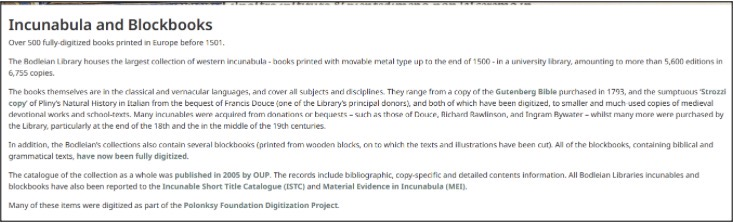
\includegraphics[width=0.5\textwidth]{./images/presentation_editorialisation/IMG_6038.jpeg}
\end{center}

\paragraph*{Organisation en focus thématiques} 

\textbf{Cariatide, bibliothèque numérique de l’INHA:}
\url{https://bibliotheque-numerique.inha.fr/focus-thematiques} 

Cariatide propose une page de focus thématiques divisée en quatre blocs successifs : les dernières parutions, les histoires de collection, puis les articles et pour finir tous les focus thématiques, dans lesquels on peut lancer une recherche et que l’on peut filtrer.

\begin{center}
	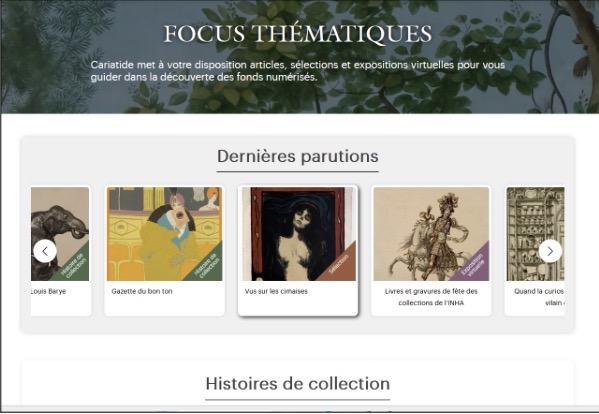
\includegraphics[width=0.5\textwidth]{./images/organisation_focus_thematiques/IMG_6040.jpeg}
\end{center}

Les focus thématiques contiennent \uline{quatre types de valorisations:} des historiques de collection, des articles, des sélections et des expositions virtuelles. Les contenus sont clairement identifiés, on sait donc à quelle catégorie appartient l’élément consulté. 

\begin{center}
	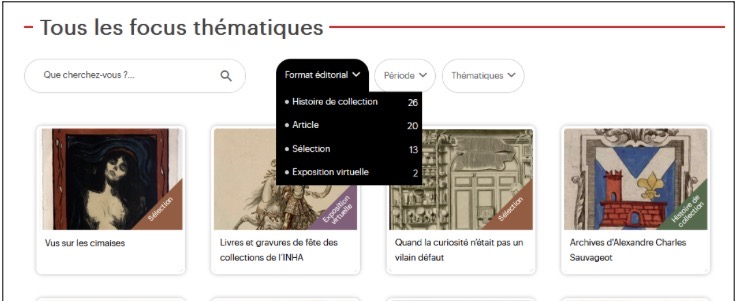
\includegraphics[width=0.5\textwidth]{./images/organisation_focus_thematiques/IMG_6041.jpeg}
\end{center}

\paragraph*{Les fonds documentaires constitués}


\textbf{Genovefa, Bibliothèque Sainte Geneviève:}
\url{https://genovefa.bsg.univ-paris3.fr/s/genovefa/page/fonds-prozor}

Genovefa éditorialise ses fonds documentaires numérisés comme on peut le constater avec le fonds Prozor. Elle indique comment la bibliothèque a pu acquérir le fonds et le nombre de documents numérisés et mis en ligne. Elle en décrit le contenu et les spécificités, afin que les lecteurs puissent en évaluer rapidement l’intérêt pour leurs recherches. 

\begin{center}
	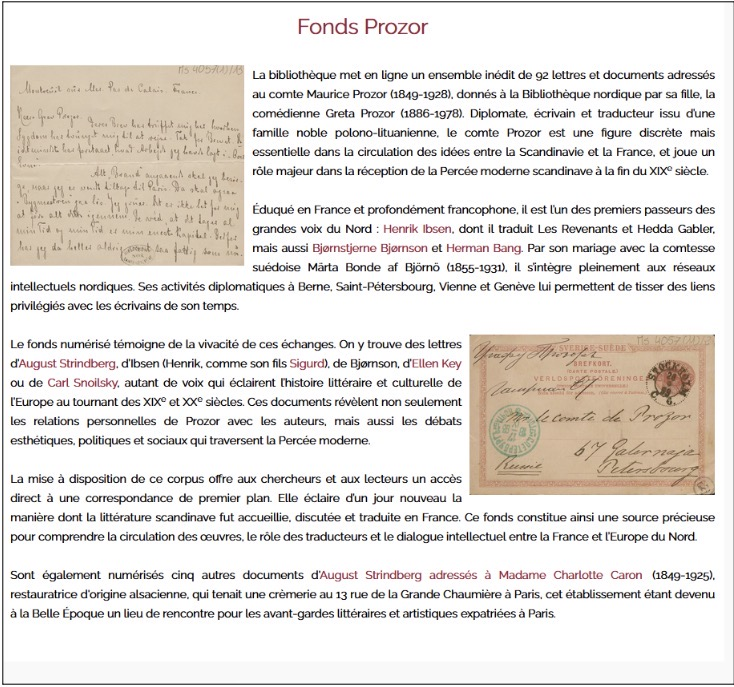
\includegraphics[width=0.5\textwidth]{./images/fonds/IMG_6042.jpeg}
\end{center}

\paragraph*{Les fiches biographiques et galeries de personnalités} 

\textbf{Lucienne, bibliothèque numérique de l’ENS:}
\url{https://lucienne.ens.psl.eu/s/lucienne/item/264210}

L’ENS a créé des fiches biographiques d’auteur dans sa bibliothèque numérique à l’intérieur de laquelle elle recense tous les documents issus de cet auteur. Cela permet une autre forme de navigation à l’intérieur du contenu numérisé dans la bibliothèque numérique.

\begin{center}
	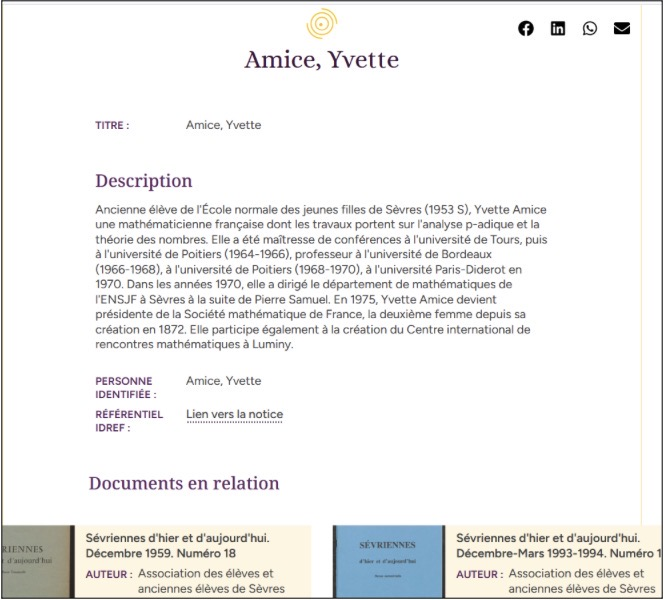
\includegraphics[width=0.5\textwidth]{./images/fiches_biographiques_et_galerie_personnalites/IMG_6043.jpeg}
\end{center}

L’ENS a aussi mis en avant une autre forme de valorisation de ses collections à travers les parcours des normalien.ne.s. Ces parcours exposent le travail de ces personnes au sein de l’institution, comme ce fut le cas pour le bibliothécaire Pierre Petitmengin.
Lucienne : https://lucienne.ens.psl.eu/s/lucienne/page/parcours-normaliens

\begin{center}
	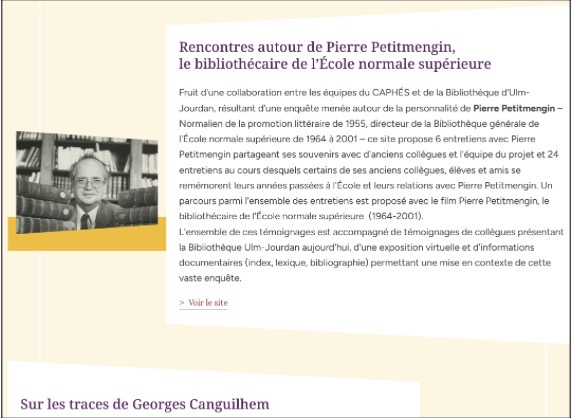
\includegraphics[width=0.5\textwidth]{./images/fiches_biographiques_et_galerie_personnalites/IMG_6044.jpeg}
\end{center}

\paragraph*{Les Expositions virtuelles :}

\textbf{NuBIS, bibliothèque numérique de la BIS:}
\url{https://nubis.bis-sorbonne.fr/expositions/}

Les responsables de NuBIS proposent aux agents qui le souhaitent de participer à la valorisation des collections numérisées. Cela permet de créer une communauté autour de la bibliothèque numérique participant ainsi à sa visibilité. Pour ce faire, deux guides pour la rédaction des billets de blog3 et des expositions virtuelles sont mis à disposition sur le site de NuBis. 

\begin{center}
	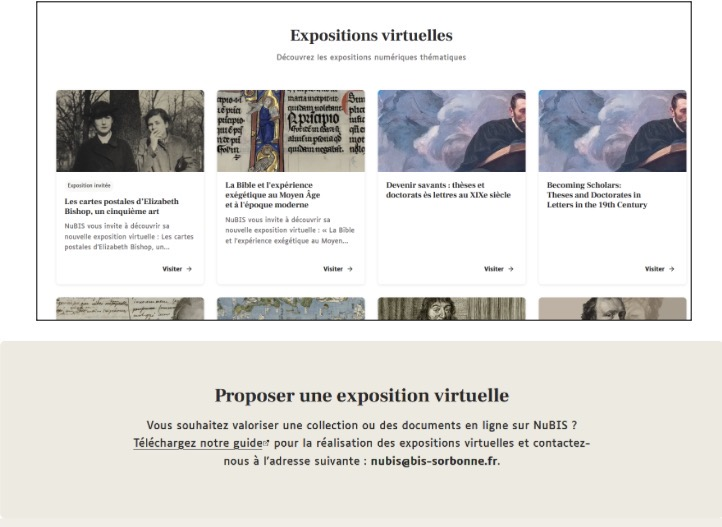
\includegraphics[width=0.5\textwidth]{./images/expositions_virtuelles/IMG_6045.jpeg}
\end{center}

\textbf{Lucienne, bibliothèque numérique de l’ENS:}
L’ENS a créé des expositions virtuelles afin de valoriser ses collections patrimoniales et de diffuser le savoir à un large public.

\begin{center}
	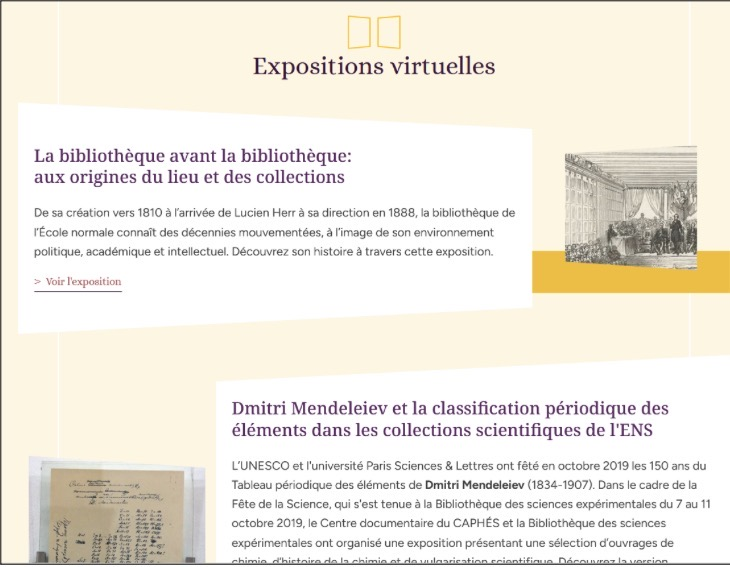
\includegraphics[width=0.5\textwidth]{./images/expositions_virtuelles/IMG_6046.jpeg}
\end{center}

\textbf{Genovefa, Bibliothèque Sainte Geneviève:}
\url{https://genovefa.bsg.univ-paris3.fr/s/genovefa/page/selections_thematiques}

Genovefa met en valeur ses collections à travers des expositions virtuelles accessibles depuis la rubrique sélection thématique. Il s’agit généralement d’une façon de prolonger en ligne une exposition ayant eu lieu à la bibliothèque. Cela permet de rattacher les documents à un contexte ou une thématique scientifique et d’attirer un plus large public.

\begin{center}
	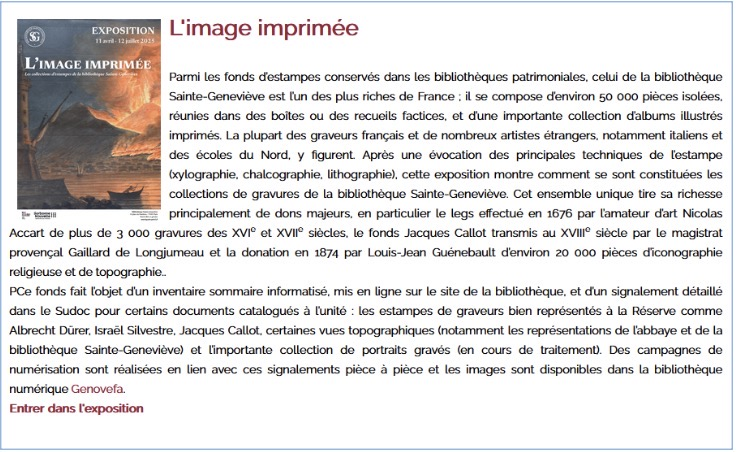
\includegraphics[width=0.5\textwidth]{./images/expositions_virtuelles/IMG_6047.jpeg}
\end{center}

\paragraph*{Présentation d’éditions numériques}

\textbf{Genovefa:} \url{https://genovefa.bsg.univ-paris3.fr/s/genovefa/page/editions_numeriques}

La BSG a comme particularité de mettre en avant les projets en Humanités numériques qui ont été menés avec les collections numérisées de l’établissement. Les projets sont présentés sous la responsabilité de l’enseignant qui en a la charge. 

\begin{center}
	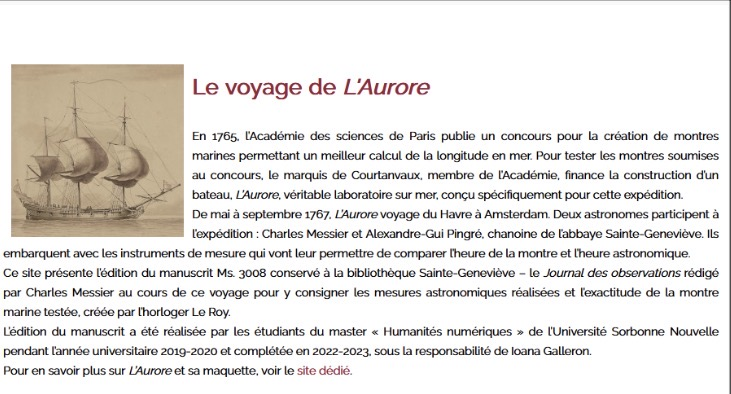
\includegraphics[width=0.5\textwidth]{./images/editions_numeriques/IMG_6048.jpeg}
\end{center}

\paragraph*{Billets de blog, actualités, lettres d’information}

\textbf{NuBIS, bibliothèque numérique de la BIS:}
\url{https://nubis.bis-sorbonne.fr/blog/}

La BIS valorise ses collections numérisées en publiant des billets de blogs à propos des documents récemment mis en ligne et de leurs auteurs. 

\begin{center}
	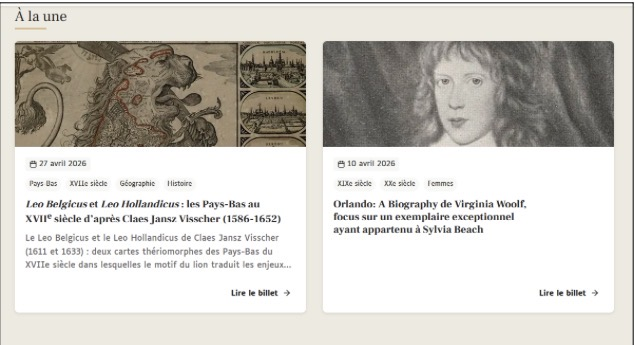
\includegraphics[width=0.5\textwidth]{./images/blog_actualites_lettres/IMG_6049.jpeg}
\end{center}

\textbf{Gallica, bibliothèque numérique de la BNF:}
\url{https://gallica.bnf.fr/accueil/fr/html/le-blog-gallica}

Gallica a mis en place différentes formes de valorisation sur son site. Le blog de Gallica relaie cette valorisation d’une autre manière, en proposant des billets qui évoquent les collections numérisées, et leur organisation en parcours thématiques. 

\begin{center}
	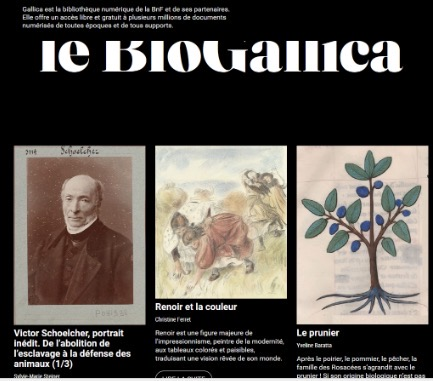
\includegraphics[width=0.5\textwidth]{./images/blog_actualites_lettres/IMG_6050.jpeg}
\end{center}

\textbf{Gallica:} \url{https://gallica.bnf.fr/accueil/fr/html/accueil-fr}

Gallica propose également une lettre d’actualité mensuelle à laquelle les usagers peuvent s’inscrire gratuitement. Cette lettre a pour objectif de fidéliser la communauté des lecteurs. Elle décrit tous les mois l’actualité de Gallica afin de permettre aux usagers de savoir quels documents ont été mis en ligne.

\begin{center}
	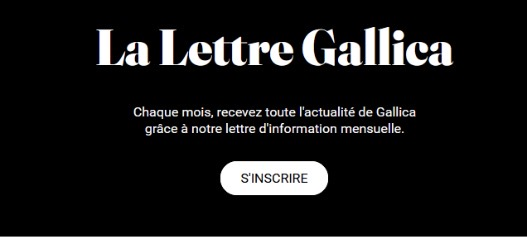
\includegraphics[width=0.5\textwidth]{./images/blog_actualites_lettres/IMG_6051.jpeg}
\end{center}

\textbf{Bibliothèque numérique de Sciences Po:}
\url{https://bibnum.sciencespo.fr/s/catalogue/page/accueil}

La bibliothèque numérique de Sciences Po met en avant son actualité en page d’accueil dans un format court et précis.

\begin{center}
	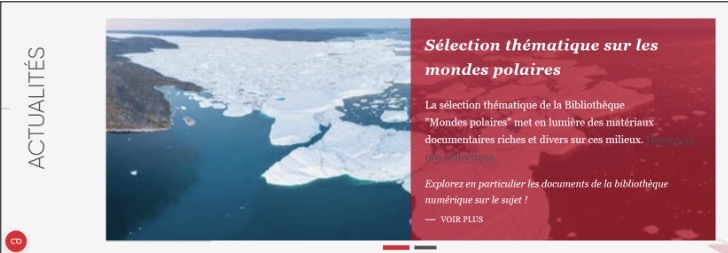
\includegraphics[width=0.5\textwidth]{./images/blog_actualites_lettres/IMG_6052.jpeg}
\end{center}

\textbf{Polona, bibliothèque numérique de la bibliothèque nationale de Pologne:}
\url{https://polona.pl/pdn/blog-entries?page=0&size=24&sort=NEWEST_PUBLICATION_DATE}

Polona présente ses actualités sous la forme de billets de blog destinés à sa communauté scientifique ou à un large public. Un filtrage est possible par thématique. 

\begin{center}
	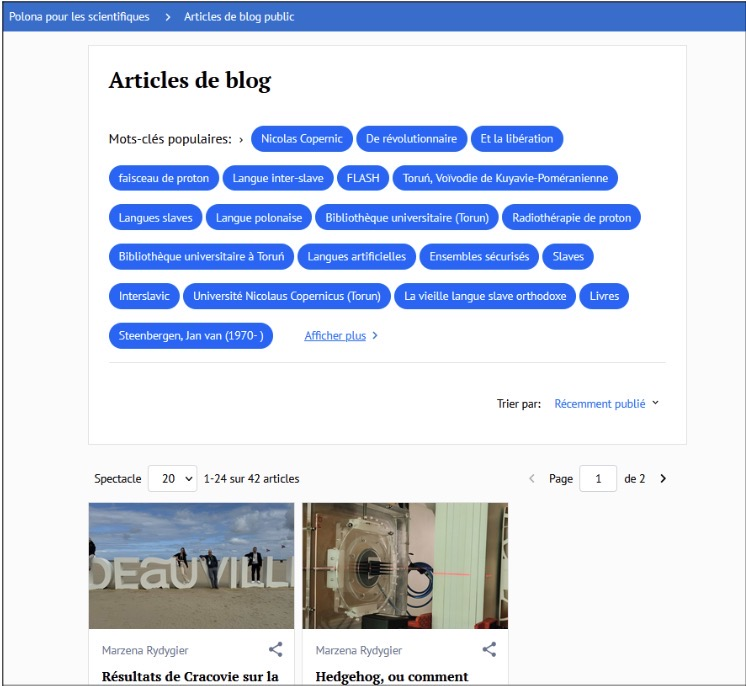
\includegraphics[width=0.5\textwidth]{./images/blog_actualites_lettres/IMG_6053.jpeg}
\end{center}

\subsubsection{Proposition pour la bibliothèque numérique de Cujas}
\begin{itemize}
	\item La bibliothèque numérique doit contenir une page à propos, une page sur les mentions légales, une page sur la politique de confidentialité (RGPD), une page sur les conditions d’utilisation, une page sur l’accessibilité et une adresse mail de contact.
\item L’accompagnement des usagers peut s’appuyer sur une foire aux questions (FAQ). Ce format, très familier pour la majorité des utilisateurs, offre des réponses simples et rapides sans alourdir la navigation dans la bibliothèque numérique. 
\item Une organisation en collections et sous-collections à trois niveaux doit être mise en place (nécessaire pour le corpus Pfister-Roumy). 
\item Des pages d’éditorialisation doivent pouvoir être ouvertes pour présenter les collections et les sous-collections, présenter les documents qui y figurent et justifier la démarche intellectuelle qui a abouti à leur création. Les textes de présentations doivent être visibles sur la page dès que l’on consulte la collection. Elles doivent comporter des images pour illustrer le type de documents que l’on va trouver.
\item Il doit être possible d’implémenter une page d’éditorialisation pour un document spécifique, depuis la page de présentation du document. 
\item L’éditorialisation des fonds peut prendre différentes formes : billets de blog écrits par des chercheurs ou des étudiants encadrés par un directeur, galerie des professeurs de Faculté de droit de Paris, expositions virtuelles ou parcours guidés. Des liens vers les expositions et plateformes créés et gérés par le SPAR doit être envisagé. Cette éditorialisation doit permettre d’améliorer la visibilité de la bibliothèque numérique, de contextualiser les documents et de les relier entre eux autour d’un thème commun, renforçant ainsi sa crédibilité scientifique et culturelle.
\item Cette organisation en collections ne doit pas être mélangée à la présentation thématique actuellement présente en page d’accueil. 
\end{itemize}

\subsubsection{Réponse aux besoins identifiés par les personae}

Afin de valider la pertinence des choix fonctionnels proposés pour la valorisation, l’information et l’accompagnement des usagers, la synthèse ci-dessous illustre commet chaque fonctionnalité répond aux besoins prioritaires des personae :
\begin{itemize}
	\item \textbf{Besoin n°1 : Explication sur la prise en main de la bibliothèque numérique :}
\begin{itemize}
	\item \uline{Personae concernés :} chercheur expert en histoire du droit, doctorante, étudiant, professionnel du droit.
\item \uline{Réponse :} Création d’une page d’aide centralisant les questions courantes concernant la prise en main de la bibliothèque numérique et des outils mis à la disposition des usagers (Mirador, IIIF, recherche simple, recherche avancée, recherche plein-texte).
\end{itemize}
\item \textbf{Besoin n°2 : Médiation culturelle des documents numérisés :}
\begin{itemize}
	\item \uline{Persona concerné :} Responsable de la bibliothèque numérique et chercheur expert en histoire du droit.
\item \uline{Réponse :} Valorisation des collections ou des documents numérisés à travers différents espaces d’éditorialisation (présentation des collections, expositions virtuelles, parcours guidés). Les enseignants-chercheurs s’informent beaucoup grâce aux actualités.
\end{itemize}
\end{itemize}

\section[Page d'accueil]{Page d’accueil et son arborescence}
\subsection{Le plan du site}

\begin{itemize}
	\item Accueil
\item Collections
\begin{itemize}
	\item Fondamentaux du droit 
\item Les cours Carbonnier
\item Les Cours de droit
\item Le fonds Pardessus
\end{itemize} 
\item Thématiques 
\begin{itemize}
	\item Codes
\item Droit civil
\item Droit coutumier
\item Droit romain
\item Droit Canonique
\item Droit commercial
\item Droit pénal
\end{itemize}
\item Recherche
\begin{itemize}
	\item Simple
\item Avancée
\item Plein-texte
\item Explorer
\end{itemize}
\item Galerie virtuelle
\begin{itemize}
	\item Galerie des professeurs
\item Hoppe Droit
\item Expositions
\end{itemize}
\item A propos
\begin{itemize}
	\item Contact
\item Aide
\item Conditions d’utilisation
\end{itemize}
\item Compte personnel
\item Contact
\item Conditions d’utilisation
\item Mentions légales
\item Plan du site 
\item Accessibilité : partiellement conforme

\end{itemize}
\subsection{Page d’accueil : maquette}

\begin{center}
	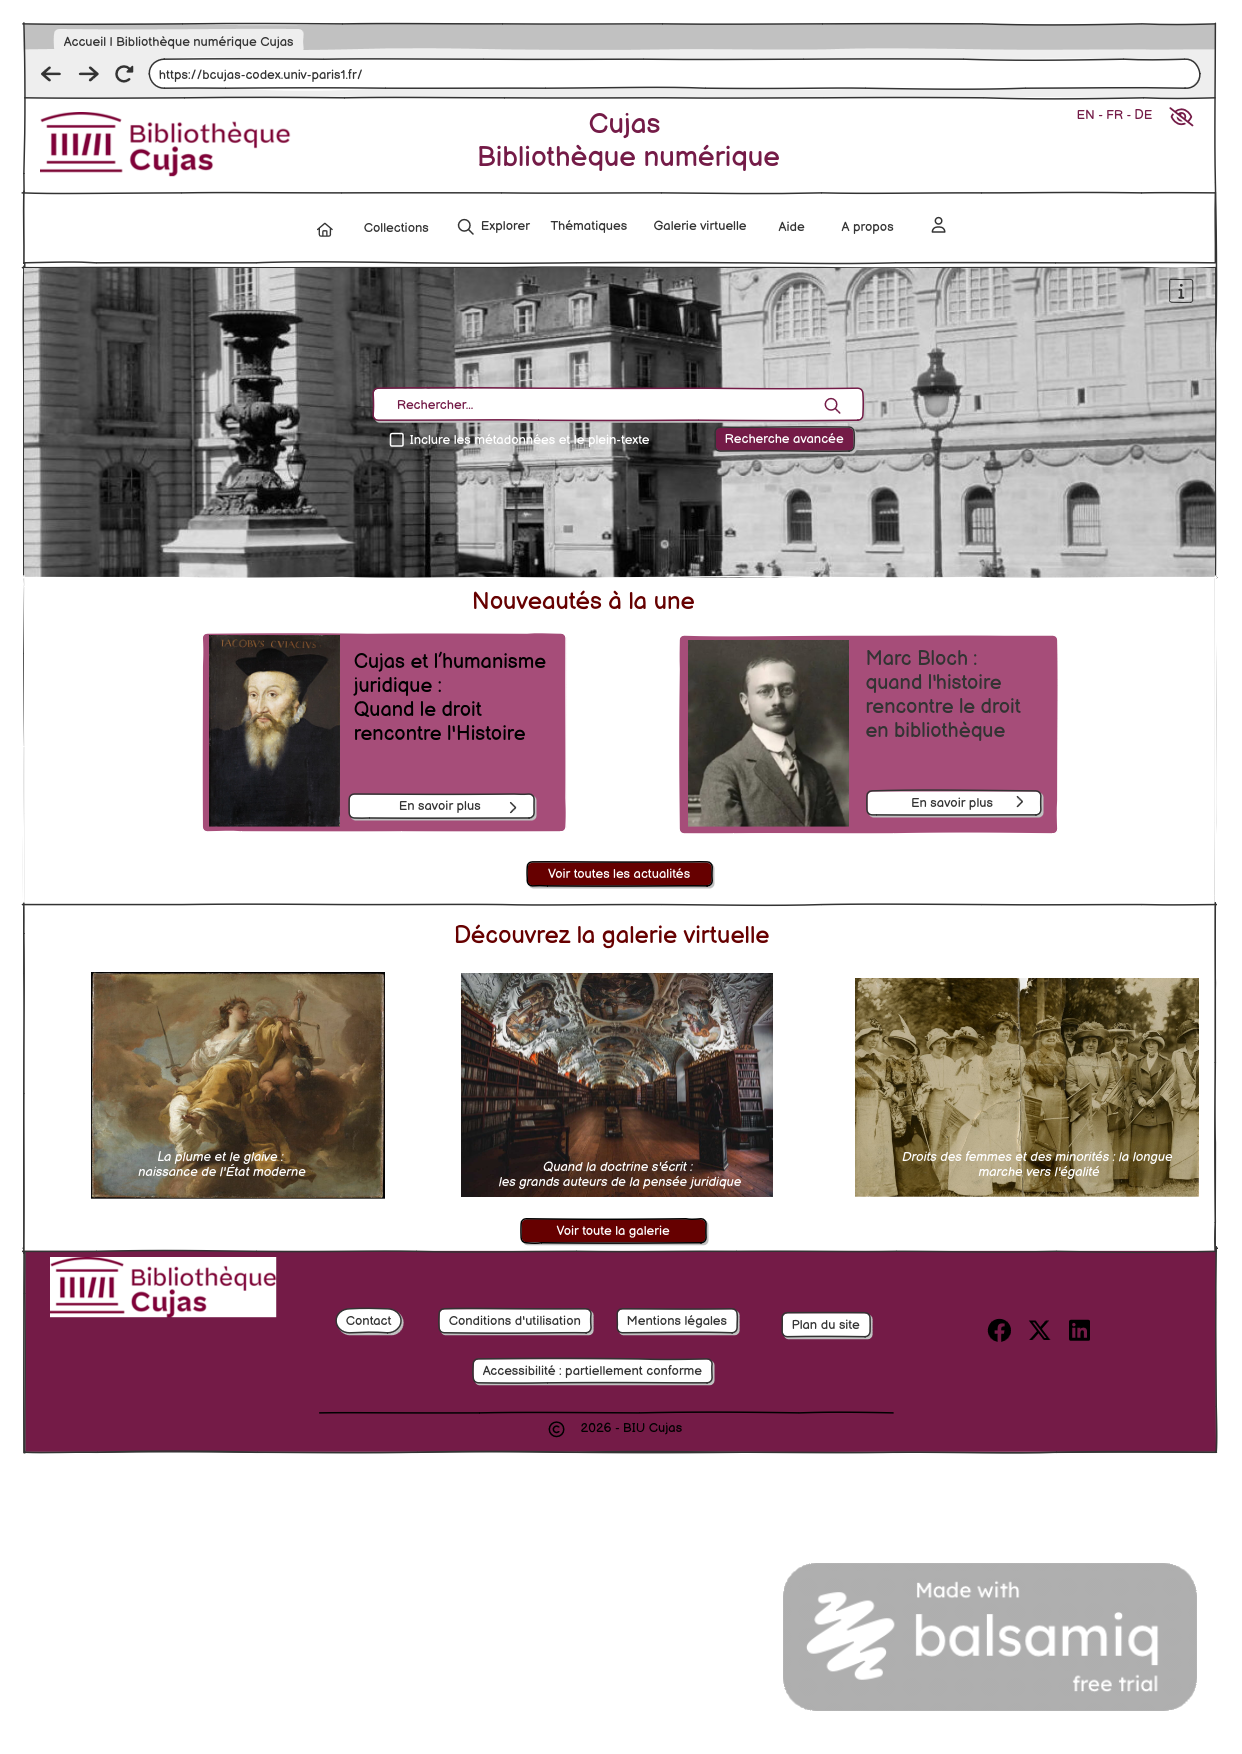
\includegraphics[width=0.9\textwidth]{./images/Page_accueil_2.pdf}
\end{center}

\section*{Conclusion}
\addcontentsline{toc}{section}{Conclusion}
\begin{itemize}
	\item Ces recommandations constituent une base de travail pour le futur cahier des charges de Codex. Certains points sont à instruire, comme les métadonnées descriptives et leur alignement avec des référentiels. Les propositions sont à préciser, valider ou modifier. 
\item Le développement de cette interface représente une belle opportunité de modernisation. Cette transition doit s’inscrire dans une démarche globale d’accompagnement des équipes afin qu’ils comprennent ces nouveaux outils et services mis à disposition des usagers. De plus, une forme éditorialisation (présentation des collections, parcours guidés, rédaction d’actualités) est attendue demandant une connaissance fine des espaces prévus à cet effet et de leur fonctionnement. Enfin, dans une logique de transmission et d’ouverture, une documentation rigoureuse est nécessaire pour s’approprier l’architecture de la plateforme.
\item En réunissant ces conditions, le prototype Codex ne sera plus uniquement un catalogue de consultation mais deviendra un véritable espace de vie intellectuelle, de médiation culturelle et de partage du savoir.
\end{itemize}


\section*{Annexes}
\addcontentsline{toc}{section}{Annexes}
\subsection*{Personae}
\addcontentsline{toc}{subsection}{Personae}

\subsubsection*{Chercheur expert en histoire du droit}
\addcontentsline{toc}{subsubsection}{Chercheur expert en histoire du droit}
Hugo

Age : 56 ans

Métier : Professeur d’histoire du droit à Paris II.

Le Chercheur Expert en Histoire du Droit.

(Archétype : enseignants-chercheurs et directeur de revue).

\paragraph*{Motivations principales:}

\begin{itemize}
	\item Avoir accès à un lieu virtuel concentré réunissant des sources du droit rare ou physiquement difficiles d’accès, pour s’éviter des déplacements fastidieux.
\item Création d’une deuxième liste Pfister-Roumy : important de numériser tous les manuels de droit civil, de procédure, commercial entre 1800 et 1940, ainsi que les revues notamment les trimestriel du droit civil crée en 1902, les grandes revues.
\item Bibliothèque numérique : lieu concentré où l’on peut trouver les sources souhaitées.
\item Développer la science ouverte
\item Rendre plus facile et accessible les collections.
\end{itemize} 

\paragraph*{Expériences / habitude de recherches:} 
\begin{itemize}
	\item Recherche plus aléatoire à travers les collections de la bibliothèque numérique comme il pourrait être amené à le faire dans une salle de lecture.
\item Apprécie la bibliothèque de Munich car possibilité de se balader dans les collections comme il le souhaite
\item Aime pouvoir faire une balade bucolique dans l’arborescence.
\item Le mode de consultation de la bibliothèque Cujas est plus commode que dans d’autres bibliothèques numériques, navigue bien dedans contrairement à Internet Archives.
\item Aime pouvoir télécharger ses documents sous format PDF.
\item Tous les documents qui l’intéressent il les a téléchargés sous format PDF afin de se constituer une arborescence à l’intérieur de son propre ordinateur afin de s’y retrouver lorsqu’il recherche un document ou un passage l’intéressant pour ses travaux.
\item Travaille par cercle concentrique sur un projet de recherche.
\end{itemize}

\paragraph*{Besoin pour la nouvelle bibliothèque:}

\begin{itemize}
	\item Si on fait une demande ciblée aimerait avoir la possibilité d’avoir d’autres résultats lorsque l’on clique sur la notice faisait référence à des travaux similaires ou quand l’auteur et ses travaux eux-mêmes peuvent être cité ailleurs.
	\item Ne pas être contraint dans sa démarche de recherche par des filtres trop précis
	\item Avoir plus de filtre permettrait de voir qu’il y a d’autres ouvrages pouvant être intéressant lui permettant d’aller plus loin.
	\item Aimerait que la navigation à l’intérieur d’un ouvrage numérique se rapproche de celui d’un ouvrage papier que l’on peut manipuler comme on le souhaite.
	\item OCR très important.
	\item Se rapprocher de la souplesse de fonctionnement d’un livre (facilité de repérages des éléments intéressants ainsi que de déplacement à l’intérieur). 
	\item Comparaison des textes à l’intérieur d’une même visionneuse ne l’a jamais utilisé lui-même mais a eu un retour d’expérience d’un collègue lui disant que c’est bien.
	\item Avoir la possibilité lorsque l’on cherche par mots-clés qui est surligné dans le texte (titre, passage dans le texte), avec la possibilité de s’y rendre directement sur la page avec le passage qui nous intéresse (exemple : comme sur Gallica).
	\item Avoir le choix de télécharger la totalité du document ou qu’une partie serait bien. Cela éviterait que cela soit trop lourd et cela serait aussi plus commode.
	\item Création d’un compte personnel lui permettant d’enregistrer ses recherches afin d’avoir un « historique », mettre en favoris, annoter. Avoir un espace à soi avec la possibilité de pouvoir répartir les sources comme il le souhaite pouvant créer des dossiers avec des sous-dossiers comme dans son ordinateur.
	\item Important d’avoir la référence bibliographique afin de l’exporter dans Zotero, évitant ainsi de devoir chercher partout les éléments devant la constituer.
	\item Avoir la possibilité de rebondir sur d’autres sites comme le Sudoc ou Calames.
	\item Intéressant de pouvoir permettre aux chercheurs d’écrire un court article permettant de mettre en avant une partie du fonds sur lequel il travaille.
	item Mettre plus en avant les collections de la bibliothèque numérique notamment lorsqu’il y a de nouvelles numérisations qui sont réalisées trouvent cela important.
	
\end{itemize}

\paragraph*{Frustration:} 

\begin{itemize}
	\item Actuellement, filtres trop précis pour l’usage qu’il souhaite en faire n’apprécie pas vraiment cette contrainte ne trouvant pas forcément cela très intéressant.
\item Il aimerait bien pouvoir prendre un chemin de traverse sinon trop réducteur.
\item Face à un ouvrage numérique, si la navigation à l’intérieur de celui-ci n’est pas facilitée par une table des matières cliquables ou de la recherche plein-texte possible (OCR). Cela rend la recherche plus fastidieuse surtout lorsque celui-ci est très volumineux.
\item Problème d’absence d’océrisation dans les textes rend impossible le repérage de mots dans le texte afin de gagner du temps. 
\item En cas d’absence d’OCR obligé de télécharger l’ouvrage et de le faire océrisé de façon approximative via Adobe professionnel. Reconnait que pour un étudiant ou un jeune chercheur cette solution n’est pas envisageable.
\item Lorsqu’il y a un zoom dans la visionneuse a dû mal à l’utiliser surtout si c’est celui où l’on peut zoomer automatiquement grâce à la molette de la souris.
\item Ne trouve pas tous les services liés à la visionneuse très commode.
\item Aime moins le format word qu’il trouve moins ergonomique.
\end{itemize}

\subsubsection*{Doctorante en histoire du droit et des institutions}
\addcontentsline{toc}{subsubsection}{Doctorante en histoire du droit et des institutions}
Ophelia 

Age : 30 ans

Métier : Maître de conférence à Paris I.

La Doctorante Experte en histoire du Droit et des institutions

(Archétype : doctorante ayant travaillé sur la bibliothèque numérique devenu maitre de conférence)

\paragraph*{Motivations principales:} 
\begin{itemize}
	\item La bibliothèque numérique possède une riche collection d’ouvrages.
\item D’avoir des tables des matières cliquables lui permettant d’avoir une aisance dans la navigation des documents numérisés. Cela se rapproche un peu de la manipulation que l’on peut avoir avec un livre papier pouvant aller directement à la section qui l’intéresse.
\end{itemize}
\paragraph*{Expériences / habitudes de recherches:}
\begin{itemize}
	\item Utiliser énormément la recherche simple moins la recherche avancée même si elle la trouve bien. 
\item Elle utilise énormément le PDF, car elle apprécie de pouvoir les annoter comme elle le souhaite, découper des passages afin de constituer ses cours sur powerpoints. 
\item Elle a l’habitude de chercher, de fouiller pour trouver le document qui l’intéresse ça fait partie de son processus de réflexion et elle apprécie pouvoir le faire.
\item Elle apprécie d’avoir la possibilité de naviguer dans le document grâce à la table des matières cliquables rendant la manipulation du texte plus agréable sans avoir à tourner chaque page pour tomber sur la partie ou la section qui l’intéresse de juste à cliquer dessus pour y avoir directement accès lui apporte un confort dans ses recherches.
\item Elle utilise aussi beaucoup quand c’est possible la recherche par occurrence dans les PDF qu’elle a téléchargé. Cela renforce la facilité de navigation et la prise en main de celui-ci et complète les tables des matières.
\end{itemize}
\paragraph*{Besoin pour la nouvelle bibliothèque:}
\begin{itemize}
	\item Elle a l’impression que les facettes n’ont pas été fait par un juriste. Après la logique est bien mais si on souhaite les conserver elle suggère de créer une arborescence à deux ou trois niveaux en fonction des thématiques afin simplifier son utilisation et sa compréhension.
\item Elle aimerait avoir un compte personnel permettant de mettre en favoris les documents recherchés, de pouvoir y revenir plus tard même si on n’a fermé le site car étant amené à consulter plusieurs fois les mêmes documents au cours de ses recherches avoir juste à revenir sur son compte. Cela apporte un confort. Cela peut être un compte comme on en trouve sur le catalogue Primo.
\item Elle aimerait bien avoir accès à la référence bibliographique déjà rédigé qu’elle n’a plus qu’à copier-coller dans son document.
\item Elle aimerait bien trouver une page d’aide dans la bibliothèque numérique, clarifiant comment prendre en main les nouveaux outils comme la visionneuse IIIF ou bien une foire aux questions disponibles recensant les questions qui sont souvent posées, y répondre en donnant accès à tous afin que si d’autres se posent les mêmes questions puissent avoir déjà la réponse.
\item Cela pourrait peut-être bien d’avoir un titre abrégé pour les étudiants lorsque le titre est latin. Ce n’est pas toujours évident pour eux de repérer les documents surtout avec les déclinaisons car tous n’ont pas forcément reçu un enseignement latiniste. Cela permettrait également au moteur de recherche de trouver les documents car si la déclinaison latine n’a pas été renseigné. Il peut arriver que le moteur de recherche ne trouve pas le document.
\item Elle apprécierait d’avoir la possibilité d’avoir le choix entre télécharger seulement une partie du document ou sa totalité comme sur Gallica.
\end{itemize}
\paragraph*{Frustrations:}
\begin{itemize}
	\item Titre des vignettes laissent sous-entendre que l’on va traiter d’une collection précise avec des ouvrages en lien avec celui-ci sauf qu’en réalité c’est moins le cas. Elle a une impression de fouillis.
\item Il manque une explication liée à la raison pour laquelle les corpus ont été construite de cette façon et non d’une autre. Elle se sent donc un peu perdue ayant du mal à comprendre pourquoi les documents ont été rassemblés de cette façon. Une explication sur les choix éviterait une confusion.
\item N’utilise pas vraiment les facettes car elles les trouvent trop précise voir inadapté à certain moment. Par exemple : quand ces dernières font référence à un document – Loi des Douze Tables – ne parvient pas dans ce cas à comprendre son utilité car pour elle si un chercheur recherche ce document il va utiliser la recherche simple pour le trouver.
\item Lorsqu’elle avait du mal à accéder à la bibliothèque numérique, elle contournait le problème en cherchant de mémoires le titre de son ouvrage dans Google tombant sur le PDF de ce dernier mais n’ayant par ce chemin d’accès aucun moyen d’aller dans la bibliothèque numérique une fois l’ouvrage consulté ou d’accéder à ses métadonnées. 
\item N’apprécie pas la manière dont le panier a été configuré surtout lorsqu’elle quitte la page et elle porte tous ses favoris. 
\end{itemize}


\subsubsection*{Etudiant en histoire du droit}
\addcontentsline{toc}{subsubsection}{Etudiant en histoire du droit}
Lucas

Age : 21 ans
 
Métier : étudiant en master 1 d’histoire du droit

Etudiant en histoire du droit

\paragraph*{Source:}
\begin{itemize}
	\item Résultat de l’enquête de terrain sur LimeSurvey
Tendance d’utilisation de la bibliothèque numérique :
\item Pour accéder à la bibliothèque numérique, ils ont tendance à utiliser soit le site de la bibliothèque Cujas, le catalogue ou encore par une recherche internet qu’ils ont effectué dans un moteur de recherche.
\item Ils utilisent principalement le PDF, la recherche simple et la recherche avancée ainsi que les tables des matières.
\end{itemize}
\paragraph*{Besoins pour Codex:}
\begin{itemize}
	\item Une visionneuse IIIF (zoom profond, visualisation aisé de documents en haute résolution, comparaison entre images, recherche plein texte...)
\item Reconnaissance automatique de texte (tous les documents ou une catégorie)
\item Exporter des références bibliographiques pouvoir soit les copier-coller soit les mettre dans un logiciel bibliographique comme Zotero, EndNote...
\item Rebondir sur une référence dans d'autres bibliothèques numériques ou catalogue (SUDOC, CALAMES, GALLICA...)
\item Avoir le choix entre plusieurs formats (PDF, TXT...)
\item Avoir la possibilité de télécharger soit une partie du document ou tout le document au format souhaité.
\item Disposer d'un compte personnel (enregistrement des recherches, mémoriser des documents dans une liste de lecture...).
\end{itemize}
\paragraph*{Frustrations:}
\begin{itemize}
	\item Dans l’ensemble, ils sont moyennement satisfaits en ce qui concerne l’organisation et la navigation dans la bibliothèque, la clarté des informations, la facilité avec laquelle on trouve un document dedans et de son design et de sa lisibilité.
\end{itemize}

\subsubsection*{L’Amatrice éclairée}
\addcontentsline{toc}{subsubsection}{L’Amatrice éclairée}
Clémence 

Age : 35 ans

Métier : Professionnel du droit

Le juriste

\paragraph*{Source:}
\begin{itemize}
	\item Résultat de l’enquête de terrain sur LimeSurvey
Tendance d’utilisation de la bibliothèque numérique :
\item Il accède généralement à la bibliothèque numérique grâce à une recherche dans le catalogue de la bibliothèque, par le site de la bibliothèque ou bien au cours d’une recherche sur Internet.
\item Ils ont tendance à consulter la visionneuse JPEG, le PDF, la recherche simple et avancée ainsi que la table des matières et par moment les collections présentes dans la page d’accueil.
\end{itemize}
\paragraph*{Besoins pour Codex:}
\begin{itemize}
	\item Une visionneuse IIIF (zoom profond, visualisation aisé de documents en haute résolution, comparaison entre images, recherche plein texte...)
\item Reconnaissance automatique de texte (tous les documents ou une catégorie)
\item Exporter des références bibliographiques pouvoir soit les copier-coller soit les mettre dans un logiciel bibliographique comme Zotero, EndNote...
\item Rebondir sur une référence dans d'autres bibliothèques numériques ou catalogue (SUDOC, CALAMES, GALLICA...)
\item Avoir le choix entre plusieurs formats (PDF, TXT...)
\item Disposer d'un compte personnel (enregistrement des recherches, mémoriser des documents dans une liste de lecture...).
\item Demande à numériser les ouvrages anciens qu’on peut certes emprunter, mais s’effritent e sur lesquels certains surlignent ou écrivent de façon scandaleuse en toute impunité.
\end{itemize}
\paragraph*{Frustrations:}
\begin{itemize}
	\item Dans l’ensemble, ils ne sont pas du tout satisfaits par la bibliothèque numérique actuellement notamment en ce qui concerne l’organisation des contenus et la navigation à l’intérieur de celle-ci, de la facilité avec laquelle on trouve le document souhaité et la clarté des informations qui les décrivent.
\item Ils semblent plutôt satisfaits en ce qui concerne les modalités de consultation et le design et la lisibilité.
\end{itemize}


\subsubsection*{Bibliothécaire} 
\addcontentsline{toc}{subsubsection}{Bibliothécaire}
Nolween
 
Age : 42 ans

Métier : Responsable des services numériques

Bibliothécaire

(Archétype : Bibliothécaire en charge du service public et de l’accompagnement)

\paragraph*{Motivations principales:}
\begin{itemize}
	\item Elle accompagne les usagers à prendre en main la bibliothèque et à les rendre autonome dans leur utilisation.
\item Elle souhaite connaitre les services proposés et leur fonctionnement.
\item Elle doit pouvoir répondre aux questions des chercheurs comme d’un plus large public.
\item Elle a à cœur d’assurer la médiation entre les documents numériques et le public.
\end{itemize}

\paragraph*{Besoins pour la nouvelle bibliothèque numérique:}
\begin{itemize}
	\item Elle a besoin d’informations claires sur le contenu, la description des documents, et des fonctionnalités de recherches fines, ainsi que des éléments explicatifs sur les modalités d’exploitation de la bibliothèque numérique
\item Elle aimerait pouvoir s’appuyer sur une page « d’Aide » ou une « FAQ » claire, avec des tutoriels ou des bulles d’aide contextuelles pour l’utilisation de la recherche avancée.
\item Elle souhaiterait pour éviter toute confusion un affichage clair des droits. Elle propose d’intégrer explicitement des mentions de droits (ex : licences Creative Commons, Domaine Public) directement sur la notice du document. Celle-ci peut être accompagnée d’une page explicative dans l’onglet aide afin d’expliquer la différence entre les deux.
\end{itemize}

\paragraph*{Frustrations:}
\begin{itemize}
	\item Elle ne veut pas perdre du temps à expliquer des fonctionnalités mal conçues ou peu intuitives.
\item Elle constate une ambiguïté concernant les droits de réutilisation des documents numériques notamment en différenciant les documents sous droit de ceux libre de droit.
\item Le moteur de recherche actuel génère énormément de « bruit », ce qui décourage les lecteurs.
\item La recherche avancée ne fonctionne pas très bien ne retournant pas les résultats espérés. 
\item Il manque de la documentation ou des fiches synthétiques permettant de comprendre les outils mis en place sur la plateforme.
\end{itemize}

\subsubsection*{Responsable de la bibliothèque numérique}
\addcontentsline{toc}{subsubsection}{Responsable de la bibliothèque numérique}
Esméralda

Age :  50 ans

Métier : responsable du patrimoine et de la numérisation

Responsable de la bibliothèque numérique

\paragraph*{Motivations principales:}
\begin{itemize}
	\item Elargir le public, car c’est la volonté de la direction d’avoir une bibliothèque capable d’agréger d’autres contenus provenant d’autres bibliothèques politiques. De plus, ils trouvent que le portail les essentiels du droit n’est pas satisfaisant pour les juristes. 
\item Elle souhaite accueillir d’autres types de documents non plus uniquement des monographies mais également des revues, des thèses, des images…
\item Etre interconnectés et interopérable.
\item Faire connaitre, créer une communauté attachée, qui revienne, participe, fasse connaître en augmentant ainsi la consultation et les propositions de collaboration pour la bibliothèque. 
\end{itemize}
\paragraph*{Côtés positifs de la bibliothèque numérique:}
\begin{itemize}
	\item On voit d’emblée qu’il s’agit d’une bibliothèque numérique de droit grâce à la page d’accueil. Celle-ci respecte la charte graphique, le nom de la bibliothèque Cujas est bien identifiable. 
\item Les cours de droit sont bien identifiés, mais ils sont séparés en deux entités : les Cours de droit et les Cours Carbonnier. 
\item La visionneuse JPEG est de bonne permettant de consulter convenablement les ouvrages numérisés.
\end{itemize}
\paragraph*{Amélioration des services:}
\begin{itemize}
	\item Rendre le site accessible en permettant de traduire la page au moins en anglais.
\item Adapter le site à des personnes handicapées (respectant les normes, permettant d’améliorer la lisibilité, facilité la lecture, de naviguer sans effort, d’avoir la possibilité aux personnes déficientes visuelles permettant d’utiliser le format Daisy).
\item Dans la bibliothèque numérique, il faudrait que l’on trouve les données des différents types de formats, des espaces de valorisation et éditorialisation, des outils de recherche ainsi que d’exploitation des données comme un lien zotero, un compte personnel, également les informations juridiques et de contact ainsi qu’un outil de statistiques pour un usage interne.
\item Dans cette nouvelle bibliothèque, il est important que les index soient à tous les nouveaux types de documents ajoutés. Les documents doivent pouvoir être consulté par types mais doivent pouvoir également être mélangé. 
\item Ce serait bien concernant la valorisation et l’éditorialisation, de prévoir à plusieurs endroits qui ne soient pas systématiques mais activables au fur et à mesure qu’on les crée. Dans ce sens, il faudrait pouvoir avoir accès au back-office afin de pouvoir faire l’éditorialisation ou exécuter des changements si jamais, il remarque une erreur, afin de la corriger. 
\item Il faudrait également qu’il y est une présentation générale en page d’accueil, ainsi qu’une présentation de chacun des corpus ou des collections avec la possibilité d’intégrer d’autres documents grâce à des ou grâce au protocole IIIF.
\item La liste des résultats lorsqu’une recherche est effectuée doit pouvoir être filtrable c’est-à-dire par ordre alphabétique grâce au nom de l’auteur, par date d’édition croissant ou décroissant et éventuellement par titres.
\item Il faudrait qu’à chaque fois que cela est possible d’adosser les données bibliographiques complètes à des référentiels et de permettre des rebonds sur les données issues de référentiels (auteur, sujet, format).
\item Il faudrait pouvoir permettre aux utilisateurs d’avoir le choix au moment du téléchargement du document, soit il décide de le télécharger en entier soit ils prennent uniquement la partie qui les intéressent.
\item Il faudrait penser à pouvoir ajouter les réseaux sociaux à l’intérieur. 
\item Créer une galerie des grands juristes : choisir des grands auteurs, écrit une présentation sur eux compris entre 5 et 10 000 signes en faisant également le lien avec les œuvres numérisées sur Cujas ou ailleurs. 
\end{itemize}
\paragraph*{Frustrations:}
\begin{itemize}
	\item Il n’est pas possible de faire de l’éditorialisation des collections ce qui participent à l’invisibilité de la bibliothèque numérique sur Internet. 
\item Les actualités sont actuellement difficilement visibles, depuis le côté droit de l’à propos, et représentent uniquement un lien vers les actualités du service sur le site Cujas. 
\item Le contenu des collections est confus, on ne sait pas si on est dans une approche thématique ou dans une approche par corpus. 
\item Le corpus des Fondamentaux du droit n’est pas mis en valeur, alors qu’il constitue la collection phare de la bibliothèque numérique et prioritairement ce qui va intéresser les utilisateurs. 
\item Elle n’a pas accès au back-office de la bibliothèque numérique ce qui donne un effet boîte noire où elle ignore ce qui se passe à l’intérieur. Elle ne voit pas comment le workflow réagit.
\item Dans la page de recherche avancée, on trouve au même endroit la possibilité de faire de la recherche avancée dans la partie intitulée notice bibliographique. Cela peut créer une confusion d’autant que la recherche avancée ne fonctionne pas très bien. La recherche en texte intégral non plus, car il faudrait qu’il y est davantage de texte océrisés dedans afin de pouvoir faire une recherche optimale.
\item Concernant le rapatriement de données pour le moment cela n’est pas faisable représentant une limitation importante. 
\item Compte tenu de la solution logiciel utilisé, c’est retrouvé isolé avec le temps par rapport au monde des bibliothèques qui a évolué, se trouvent déconnecté de la communauté.
\end{itemize}

\subsubsection*{Informaticien}
\addcontentsline{toc}{subsubsection}{Informaticien}
Thomas

Age : 45 ans

Métier : Responsable du service informatique

L’Informaticien

Archétype : le gestionnaire de l’infrastructure, garant de la sécurité, de la pérennité des 
données et de l’interopérabilité.

\paragraph*{Motivations principales:}
\begin{itemize}
	\item L'interopérabilité avant tout : Concevoir un système ouvert reposant sur des standards internationaux non propriétaires (XML, JSON, RDF, EAD, JPEG 2000, TIFF, PDF/A) pour faciliter les échanges.
\item L'automatisation des flux : Soulager le personnel humain en automatisant un maximum de tâches de traitement (génération d'identifiants ARK, création de métadonnées DC/METS, transferts SFTP), particulièrement la nuit pour éviter les surcharges réseau.
\item La pérennité et la sécurité des données : Assurer un archivage pérenne des fichiers maîtres (TIFF) au CINES via la création automatique de paquets SIP, pour préserver la matière première et permettre de futurs retraitements (comme l'amélioration de l'OCR).
\end{itemize}
\paragraph*{Expériences / Habitudes de travail (L'existant):}
\begin{itemize}
	\item Il a construit "ArcNum" (en Python), un script automatisé complexe qui gère la chaîne de traitement (workflow) de la validation à la publication, en passant par de multiples serveurs de stockage (118, 134, NAS).
\item Il doit gérer l'héritage de CujasNum, basé sur XTF : une technologie choisie par défaut vers 2008 car c'était la seule capable de gérer des livres électroniques océrisés, mais qui fonctionne de manière très rigide (sans véritable back-office, où tout ce qui est versé est immédiatement publié).
\end{itemize}
\paragraph*{Besoins techniques pour Codex:}
\begin{itemize}
	\item Une architecture modulaire et API : Le système doit reposer sur des modules communicants et exposer ses données via des API REST (nécessitant parfois des clés de connexion) et le protocole OAI-PMH pour le moissonnage externe.
\item Une gestion fine des données : Le système doit être capable de modéliser des hiérarchies complexes (comme pour les périodiques : Titre > Année > Fascicule > Article) et de regrouper les documents en "sets" (par sujet, par lots, par classification Dewey) pour un moissonnage sélectif.
\item Une gestion centralisée des accès : Intégrer nativement les protocoles d'authentification (SSO, SAML via Shibboleth ou Renater) pour donner accès aux documents sous droits uniquement au réseau de l'université ou sur place.
\item Un back-office avec des rôles précis : Mettre en place un système de gestion des rôles (archiviste, catalogueur, éditeur de contenu, validateur) permettant à chacun d'agir de façon autonome sans dépendre systématiquement du service informatique.
\item L'intégration du standard IIIF : Séparer la gestion des images du reste en utilisant un serveur IIIF dédié, qui fournira les images et les manifestes pour alimenter la bibliothèque, sans dupliquer les fichiers.
\end{itemize}
\paragraph*{Frustrations et Contraintes:}
\begin{itemize}
	\item La dette technique et la rigidité : Dans le système XTF actuel, il est impossible de créer des collections ou des expositions facilement ("pas de back-office"), ce qui rend l'interface figée.
\item Les limites de performance : Les fichiers PDF actuels sont extrêmement lourds (300 à 400 Go) ce qui fait planter les téléchargements des usagers.
\item Les erreurs humaines bloquantes : Le "maillon faible" de son architecture très automatisée reste l'intervention humaine lors des corrections ; une erreur de validation bloque la chaîne d'archivage automatique vers le CINES et oblige à faire des mises à jour coûteuses en temps.
\item Le défi de la maintenance : Il doit trouver une solution pour structurer les cycles de mises à jour de la future plateforme sans impacter l'accès des lecteurs et sans générer une nouvelle dette technique pour les équipes futures.
\end{itemize}

\newpage{\pagestyle{empty}\cleardoublepage}

%%%%%%%%%%%%%%%%%%

\backmatter % glossaire, index, table des figures, table des matières.. (la bibliographie a déjà été appelée)

\printglossaries
%	\listoftables
%\listoffigures
\tableofcontents
\end{document}
